\documentclass[12pt]{book}

\usepackage[italian]{babel}
\usepackage{a4wide}
\usepackage{amsmath}
\usepackage{amsthm}
\usepackage{color}
\usepackage{graphicx}
\usepackage{epsfig}
\usepackage{fancyhdr}    % Fancy Header and Footer
\usepackage{txfonts}     % Public Times New Roman text & math font
%\usepackage{showkeys}
\usepackage[all]{xy}

%\lstloadlanguages{Java}
%\lstset{language=Java, basicstyle={\texttt\small}, stringspaces=false}
%\lstset{keywordstyle={\small\textbf}}
%\lstset{identifierstyle={\small\textsf}}

%%% Fancy Header %%%%%%%%%%%%%%%%%%%%%%%%%%%%%%%%%%%%%%%%%%%%%%%%%%%%%%%%%%%%%%
% Fancy Header Style Options
\pagestyle{fancy}                      % Sets fancy header and footer
\fancyfoot{}                           % Delete current footer settings
\renewcommand{\chaptermark}[1]{        % Lower Case Chapter marker style
  \markboth{\chaptername\ \thechapter.\ #1}{}}
\renewcommand{\sectionmark}[1]{        % Lower case Section marker style
  \markright{\thesection.\ #1}}        %
\fancyhead[LE,RO]{\bfseries\thepage}   % Page number (boldface) in left on even
                                       % pages and right on odd pages
\fancyhead[RE]{\bfseries\leftmark}     % Chapter in the right on even pages
\fancyhead[LO]{\bfseries\rightmark}    % Section in the left on odd pages
\renewcommand{\headrulewidth}{0.3pt}   % Width of head rule

%%% Clear Header %%%%%%%%%%%%%%%%%%%%%%%%%%%%%%%%%%%%%%%%%%%%%%%%%%%%%%%%%%%%%%
% Clear Header Style on the Last Empty Odd pages
\makeatletter
\def\cleardoublepage{\clearpage\if@twoside \ifodd\c@page\else%
    \hbox{}%
    \thispagestyle{empty}%             % Empty header styles
    \newpage%
    \if@twocolumn\hbox{}\newpage\fi\fi\fi}
\makeatother

\newcommand{\e}{\`e }
\newcommand{\E}{\`E }
\newcommand{\nec}{n\'e }
\newcommand{\Nec}{N\'e }
\newcommand{\cioe}{cio\`e }
\newcommand{\Cioe}{Cio\`e }
\newcommand{\piu}{pi\`u }
\newcommand{\Piu}{Pi\`u }
\newcommand{\cosi}{cos\`{\i} }
\newcommand{\Cosi}{Cos\`{\i} }
\newcommand{\poiche}{poich\'e }
\newcommand{\Poiche}{Poich\'e }
\newcommand{\purche}{purch\'e }
\newcommand{\Purche}{Purch\'e }
\newcommand{\perche}{perch\'e }
\newcommand{\Perche}{Perch\'e }

\newcommand{\st}[1]{{\tau[\![{#1}]\!]}}
\newcommand{\se}[2]{{\tau^{#1}[\![{#2}]\!]}}
\newcommand{\inter}[1]{{[\![{#1}]\!]}}
\newcommand{\gen}[1]{{\gamma[\![{#1}]\!]}}
\newcommand{\gentwo}[2]{{\gamma^{{#1}}[\![{#2}]\!]}}
\newcommand{\gentwotwo}[2]{{\gamma^{{#1}}\left[\!\left[{#2}\right]\!\right]}}
\newcommand{\gentest}[1]{{\gamma^{\mathit{test}}[\![{#1}]\!]}}
\newcommand{\sig}[2]{{\tau^{#1}[\![{#2}]\!]}}
\newcommand{\nullable}{\mathsf{nullable}}
\newcommand{\first}{\mathsf{first}}
\newcommand{\follow}{\mathsf{follow}}
\newcommand{\lfp}{\mathit{lfp}}
\newcommand{\idot}{.\,}
\newcommand{\vars}[1]{{\mathsf{vars}[\![{#1}]\!]}}
\newcommand{\declared}[1]{{\mathsf{declared}[\![{#1}]\!]}}
\newcommand{\used}[1]{{\mathsf{used}[\![{#1}]\!]}}
\newcommand{\cdc}{\vdash^{\mathsf{cdc}}}

\definecolor{lightgrey}{rgb}{0.8,0.8,0.8}

\newcommand{\javatip}[1]{
  \begin{center}
  \begin{tabular}{cc}
  \hspace*{-0.5cm}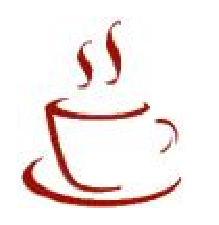
\epsfig{file = javacup.ps, width = 1.3cm}\hspace*{0.5cm} &
  {\small\colorbox{lightgrey}{\begin{minipage}{13cm}{#1}\end{minipage}}}
  \end{tabular}
  \end{center}
}

\newcommand{\greycomment}[1]{
  \begin{center}
  \begin{tabular}{cc}
  \hspace*{-0.5cm}
\epsfig{file = questionmark.ps, width = 1.3cm}\hspace*{0.5cm}
  {\small\colorbox{lightgrey}{\begin{minipage}{13cm}{#1}\end{minipage}}}
  \end{tabular}
  \end{center}
}

\newcommand{\greycommens}[1]{
  \begin{center}
  \hspace*{-0.5cm}
\epsfig{file = questionmark.ps, width = 1.3cm}\hspace*{0.5cm}
  {\small\colorbox{lightgrey}{\begin{minipage}{13cm}{#1}\end{minipage}}}
  \end{center}
}

\theoremstyle{definition}
\newtheorem{definition}{Definizione}
\newtheorem{proposition}{Proposizione}
\newtheorem{exercise}{Esercizio}

\begin{document}

\begin{titlepage}
\title{\Huge{\textbf{Un Compilatore a Oggetti per Kitten}}}
\author{{\Large{\textbf{Fausto Spoto}}}\\{\normalsize\textit{Dipartimento di Informatica}}\\{\normalsize\textit{Universit\`a di Verona}}}
\end{titlepage}
\date{\vspace*{10ex}\begin{center}
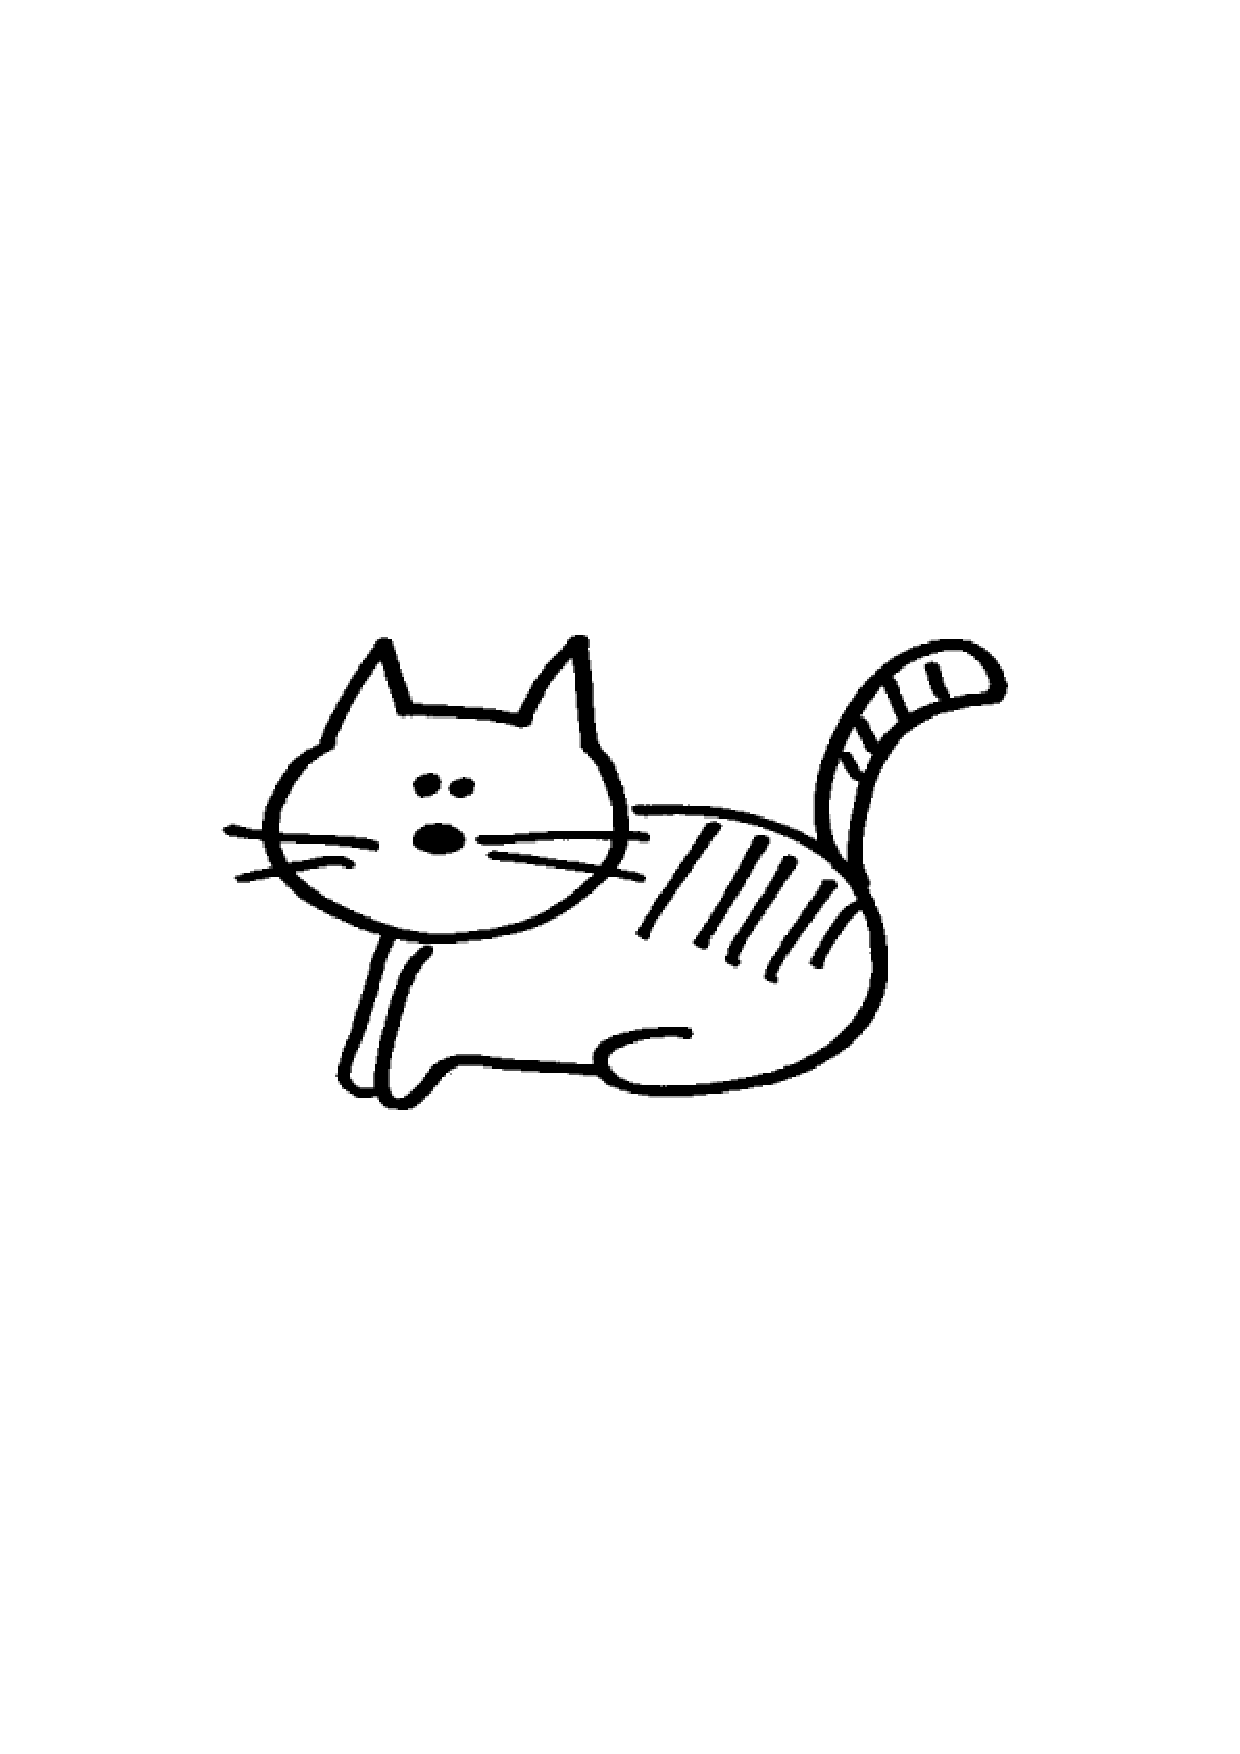
\includegraphics[width=7cm]{cat1.pdf}
\end{center}
}

\maketitle


%%%%%%%%%%%%%%%%%%%%%%%%%%%%%%%%%%%%%%%%%%%%%%%%%%%%%%%%%%%%%%%%%%%%%%%%%%%%%%%
%   Dedication Page                                                           %
%%%%%%%%%%%%%%%%%%%%%%%%%%%%%%%%%%%%%%%%%%%%%%%%%%%%%%%%%%%%%%%%%%%%%%%%%%%%%%%
\thispagestyle{empty}
\newenvironment{dedication}
  {\cleardoublepage \thispagestyle{empty} \vspace*{\stretch{1}} \begin{center} \em}
  {\end{center} \vspace*{\stretch{3}} \clearpage}

%\begin{dedication}
%A Futamura.
%\end{dedication}
% \cleardoublepage generates one blank page for the next 'Abstract'
% to be on an odd page.
%\thispagestyle{empty} \cleardoublepage

%%%%%%%%%%%%%%%%%%%%%%%%%%%%%%%%%%%%%%%%%%%%%%%%%%%%%%%%%%%%%%%%%%%%%%%%%%%%%%%
%   Abstracts                                                                 %
%%%%%%%%%%%%%%%%%%%%%%%%%%%%%%%%%%%%%%%%%%%%%%%%%%%%%%%%%%%%%%%%%%%%%%%%%%%%%%%

\mbox{}\\
\newpage
\pagenumbering{roman} \setcounter{page}{1}
\chapter*{Presentazione\markboth{Presentazione}{Presentazione}}

Scrivere un nuovo libro per un corso di compilazione sembra
un'operazione persa in partenza. \`E da venti anni che il
\emph{dragon book} di Aho, Sethi e Ullman~\cite{AhoSU86}
rimane sul mercato come
l'unico e insostituibile riferimento per chi si cimenta nella rara
e tuttora difficile arte di scrivere un compilatore. Ma gli anni passano
ed ecco che da una parte i corsi di laurea relegano la compilazione
nello spazio di poche lezioni; dall'altra l'evoluzione tecnologica dei
linguaggi di programmazione rende il \emph{dragon book} carente quanto
al trattamente della compilazione dei linguaggi \emph{a} oggetti
e della stessa compilazione \emph{con} gli oggetti. Perch\'e
la diffusione dei linguaggi a oggetti non \`e stata un cambiamento di
facciata per quanto riguarda il mondo dei compilatori: essa valorizza
il sistema di tipaggio del linguaggio; richiede
di spostare a tempo di esecuzione controlli e legami altrimenti
effettuati a tempo di compilazione; rende desiderabili nuove tecniche
di analisi e ottimizzazione del codice; infine, la stessa
implementazione a oggetti di un compilatore
rende pi\`u credibile la sua correttezza e permette l'implementazione
di ottimizzazioni tramite specializzazioni di classi e metodi della
sintassi astratta.

Ecco quindi nascere la necessit\`a di questo libro sulla
compilazione a oggetti di un linguaggio a oggetti. Non mancano certo
altri tentativi in questa direzione. Fra i tanti, non possiamo dimentivare
il libro di Appel~\cite{Appel02},
che ha inizialmente ispirato questo testo. Ma le
nostre soluzioni per il tipaggio statico e la generazione del codice
non sono assolutamente assimilabili alle tecniche dell'Appel, scarsamente a oggetti.

Questo libro si offre come supporto allo studente impegnato in un corso
di compilazione che a Verona \`e organizzato in appena
una quarantina di ore
di lezione, laboratorio incluso. Le scelte
che hanno guidato la selezione degli argomenti trattati sono quelle
dell'utilizzo intensivo della programmazione a oggetti; dell'evidenziazione
continua della relazione biunivoca fra teoria e implementazione di
un compilatore; della maggiore
importanza data alle fasi avanzate della compilazione,
come controllo dei tipi e generazione del codice,
rispetto alle prime fasi di analisi lessicale e sintattica.

Un ringraziamento va agli studenti che hanno seguito a Verona
il mio corso di compilazione negli ultimi anni. \`E dall'interazione
che ho avuto con loro che deriva la presentazione degli argomenti trattati
in questo libro. Sono loro e i loro dubbi che mi hanno spinto a
scrivere un libro e del codice che fosse
facilmente comprensibile e meno ambiguo possibile.
La scarsa presenza di bug nel compilatore Kitten \`e il risultato
della loro, spesso involontaria, verifica.

{\flushright Fausto Spoto\\\hfill Verona, gennaio 2007}

La revisione di questo testo e del compilatore Kitten ha comportanto una
semplificazione del codice e della sua presentazione, nonch\'e
la sostituzione dei makefile con dei task Ant. Il risultato sono
un compilatore Kitten e un libro pi\`u semplici e accessibili per
gli studenti.

{\flushright Fausto Spoto\\\hfill Verona, marzo 2015}

%%%%%%%%%%%%%%%%%%%%%%%%%%%%%%%%%%%%%%%%%%%%%%%%%%%%%%%%%%%%%%%%%%%%%%%%%%%%%%%
%   Acknowledgements                                                          %
%%%%%%%%%%%%%%%%%%%%%%%%%%%%%%%%%%%%%%%%%%%%%%%%%%%%%%%%%%%%%%%%%%%%%%%%%%%%%%%
%\chapter*{Acknowledgements\markboth{Acknowledgements}{Acknowledgements}}
%Your acknowledgement goes here...

%%%%%%%%%%%%%%%%%%%%%%%%%%%%%%%%%%%%%%%%%%%%%%%%%%%%%%%%%%%%%%%%%%%%%%%%%%%%%%%
%   Contents and Lists                                                        %
%%%%%%%%%%%%%%%%%%%%%%%%%%%%%%%%%%%%%%%%%%%%%%%%%%%%%%%%%%%%%%%%%%%%%%%%%%%%%%%
\newpage
%\renewcommand{\contentsname}{Indice}  % Original name = Contents
\tableofcontents
\cleardoublepage

%%%%%%%%%%%%%%%%%%%%%%%%%%%%%%%%%%%%%%%%%%%%%%%%%%%%%%%%%%%%%%%%%%%%%%%%%%%%%%%
%   Arabic numbering after this                                               %
%%%%%%%%%%%%%%%%%%%%%%%%%%%%%%%%%%%%%%%%%%%%%%%%%%%%%%%%%%%%%%%%%%%%%%%%%%%%%%%
\pagenumbering{arabic} \setcounter{page}{1}


\chapter{Introduzione a Kitten}\label{ch:kitten}
\begin{center}
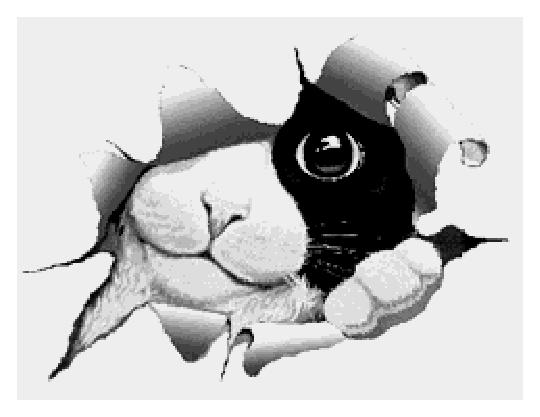
\epsfig{file = cat4.ps, width = 4cm}
\end{center}
%
Kitten \`e il linguaggio di programmazione di cui in questo libro
vogliamo descrivere un compilatore scritto in Java.
Bench\'e quindi questo libro non sia centrato solo su
Kitten, \`e necessario cominciare a
prendere familiarit\`a con tale linguaggio, in modo da essere
coscienti di quello che \`e lo scopo del nostro compilatore.
Il fine di questo capitolo \`e di descrivere l'installazione del compilatore
Kitten e il linguaggio Kitten stesso. Il compilatore ci permetter\`a di
compilare ed eseguire tutti i programmi Kitten
di esempio che incontreremo in queste pagine.

Kitten \e un semplice linguaggio di programmazione imperativo a oggetti.
\E un linguaggio \emph{imperativo} \poiche
l'esecuzione dei programmi Kitten consiste in una sequenza di passi
specificati da \emph{comandi} e ciascun comando determina una modifica
dello stato dell'esecutore. \E un linguaggio \emph{a oggetti} \poiche
lo stato dell'esecutore lega le variabili del programma a degli \emph{oggetti}
appunto, \cioe zone di memoria contenenti informazioni e che reagiscono
all'invocazione di \emph{metodi}. Va detto che Kitten non \`e un linguaggio
a oggetti \emph{puro}, nel senso che alcune variabili possono non essere legate
a oggetti, ma piuttosto a \emph{valori primitivi}. Esempi di valori primitivi
sono gli interi e i numeri in virgola mobile. Esistono pochissimi linguaggi di
programmazione puramente ad oggetti. In particolare, va ricordato
Smalltalk~\cite{GoldbergR89}. Java~\cite{GoslingJSB05}
non \`e puramente ad oggetti, perch\'e anch'esso ha dei tipi primitivi
(che per\`o coesistono con
delle versioni ad oggetti dei tipi primitivi, \cioe le \emph{classi
involucro} tipo \texttt{java.lang.Integer} e simili).
Il motivo per cui i linguaggi ad oggetti tendono a non essere puri
\`e che i valori primitivi sono gestibili molto pi\`u efficientemente
che gli oggetti.

Possiamo immaginare Kitten come una versione semplificata di Java,
sia da un punto di vista sintattico che semantico. Lo scopo di Kitten \e
infatti quello di essere un linguaggio abbastanza semplice da potere essere
compilato ed eseguito senza eccessive complicazioni, ma al contempo
sufficientemente rappresentativo dei problemi che si presentano nella
compilazione dei linguaggi di programmazione attuali tipo Java.
In Kitten mancano all'appello aspetti \emph{secondari} di Java, come
\emph{i modificatori di visibilit\`a} (\texttt{public}, \texttt{protected},
\texttt{private}), i metodi e i campi \texttt{static}, le classi
astratte e le interfacce, i package, i campi costanti, le eccezioni
e i finalizzatori.

\greycomment{Lo studente potrebbe domandarsi perch\'e non si \`e scelto
Java come linguaggio da compilare, al posto di Kitten. In fin dei conti,
Kitten non \`e utilizzato se non in questo corso e quindi la sua importanza
decade con il corso stesso. Il motivo \`e che la compilazione di Java
\`e estremamente complessa per essere descritta in un breve corso
di compilazione essendo Java, come abbiamo visto, molto pi\`u complicato
di Kitten. \`E invece pi\`u interessante chiedersi perch\'e non si
sia scritto un compilatore Kitten \emph{in Kitten}. Questo ci avrebbe
permesso, per esempio, di compilare il nostro compilatore con se stesso!
Il motivo questa volta \`e che Kitten \`e troppo povero per permettere
la definizione di un compilatore senza eccessivi sforzi di programmazione.
Per esempio, l'assenza dei modificatori di visibilit\`a e
del \emph{constructor chaining} priva la gerarchia delle classi di
ogni potere di incapsulazione, aprendo la strada a codice criptico
e scarsamente controllabile.
L'assenza dei package impedisce ogni strutturazione del progetto.
Va inoltre ricordato che esistono e che utilizzeremo degli
strumenti di sviluppo di compilatori scritti in Java, come JLex
(Capitolo~\ref{chap:lexical}) e JavaCup
(Capitolo~\ref{chap:syntactical}), e che tali strumenti andrebbero riscritti
ex-novo in Kitten.}
%
\section{Il compilatore Kitten}\label{sec:kitten_compiler}
%
Il compilatore Kitten \e scritto in Java. Si tratta, allo stato attuale, di
uno strumento che permette di compilare dei sorgenti Kitten trasformandoli
in file \texttt{.class} eseguibili da una qualsiasi Java virtual machine.
Conseguentemente, sia il compilatore Kitten che il risultato della
compilazione dei sorgenti Kitten possono essere eseguiti su qualsiasi
architettura e sistema operativo, \purche sia installato un compilatore
e interprete Java. Le istruzioni che seguono sono pensate per un'architettura
basata su Unix, tipo Linux. La compilazione sotto Windows del compilatore
Kitten \e possibile ma \e non ancora stata automatizzata.

Supponiamo di avere scaricato il file di installazione del compilatore
Kitten. Esso sar\`a un file dal nome \texttt{kitten\_XXX.tgz}, dove
\texttt{XXX} \e la versione del compilatore Kitten che si sta installando.
Tale file dovr\`a essere posizionato nel punto in cui si vuole installare
il compilatore.
Basta quindi dare i seguenti comandi per installarlo:
%
\begin{verbatim}
tar -zxf kitten_XXX.tgz
cd kitten_XXX
make generatejb
\end{verbatim}
%
Con il primo comando scompattiamo il file di installazione. Con il secondo
entriamo nella directory \cosi creata. Con il terzo compiliamo il
compilatore.
Se non \e stato segnalato alcun errore, il compilatore Kitten \e a questo
punto utilizzabile.
%
\section{Il nostro primo programma Kitten}\label{sec:first_kitten_programme}
%
\begin{figure}[t]
\begin{verbatim}
                            class Miao {
                              method void main() {
                                "miao\n".output()
                              }
                            }
\end{verbatim}
\caption{Un programma Kitten che stampa una stringa e termina.}
  \label{fig:miao}
\end{figure}

La Figura~\ref{fig:miao} mostra un esempio di programma Kitten. Si tratta
di un programma che, una volta compilato ed eseguito, stampa a video la
stringa \texttt{miao} seguita da un ritorno carrello.
Supponiamo di avere inserito il programma
in Figura~\ref{fig:miao} dentro a un file testo di nome
\texttt{Miao.kit} che si trova nella sottodirectory
\texttt{testcases} della directory \texttt{kitten\_XXX}.
La sottodirectory \texttt{testcases} \e quella che utilizzeremo
per i nostri esperimenti, in modo da non sporcare la directory
principale di Kitten. Essa non ha comunque nulla di speciale:
potevamo scegliere un qualsiasi altro nome. \E invece importante
che il nome del file \texttt{Miao.kit} termini con \texttt{.kit}.
In caso contrario esso non verr\`a riconosciuto dal compilatore
come un file testo che contiene un sorgente Kitten.
Si entri quindi nella sottodirectory \texttt{testcases}.
La compilazione del nostro primo programma Kitten si ottiene scrivendo
%
\begin{verbatim}
java -cp .. Kitten Miao.kit
\end{verbatim}
%
Questo comando chiama l'interprete Java chiedendo di eseguire un
programma di nome \texttt{Kitten}. Si tratta del compilatore Kitten che
abbiamo appena compilato.
Dal momento che esso si trova dentro la directory \texttt{kitten\_XXX},
siamo costretti a indicare che i file Java devono essere cercati in tale
directory, \cioe nella directory padre di \texttt{testcases}, in cui
siamo. Questo si ottiene con lo switch \texttt{-cp ..} che specifica
il \emph{classpath} per l'interprete Java.
Infine passiamo un parametro al compilatore Kitten. Si tratta del
nome del file che contiene il programma Kitten che vogliamo compilare.
In questo caso, si tratta di \texttt{Miao.kit}, il file sorgente Kitten da
compilare.

Il precedente comando
\e \cosi frequente che \e stata prevista una macro per semplicarne
l'esecuzione. Basta infatti digitare
%
\begin{verbatim}
./compile Miao.kit
\end{verbatim}
%
per ottenere esattamente lo stesso effetto. Si noti che, per ulteriore
semplificazione, questa macro deve essere invocata dalla directory
\texttt{kitten\_XXX} e non da \texttt{testcases}.

In ogni caso, se tutto \e andato a posto, il compilatore Kitten dovrebbe
aver compilato il file in Figura~\ref{fig:miao} comunicando a video delle
informazioni del tipo:
%
\begin{verbatim}
Parsing and type-checking completed             [419ms]
Translation into Kitten bytecode completed      [66ms]
Kitten bytecode dumping in dot format completed [15ms]
Java bytecode generation completed              [478ms]
Total compilation time was 964ms
\end{verbatim}
%
La prima riga ci informa che Kitten ha effettuato un'analisi sintattica
(\emph{parsing}) sul file \texttt{Miao.kit}, al fine di garantire che non
contenga errori di sintassi. A questa fase ne \`e seguita una di verifica
semantica (\emph{type-checking}). Il tutto ha richiesta $419$ millisecondi.
A queste due fasi ne \`e seguita una in cui il nostro programma \`e
stato tradotto in un linguaggio chiamato \emph{Kitten bytecode}. Si tratta
di un linguaggio molto simile al Java bytecode, sul quale \`e possibile
ragionare per effettuare eventuali ottimizzazioni. Tale bytecode \`e
stato anche salvato su disco in formato \texttt{dot}, un
formato di descrizione di grafi che ci permette di visionare il risultato
di questa fase della compilazione. Infine, il Kitten bytecode \`e stato
tradotto in Java bytecode, il quale pu\`o finalmente essere eseguito.

Sono tre i file che sono stati in effetti compilati in Java
bytecode. Oltre a \texttt{Main.kit}, come ci aspettavamo, ci sono anche
\texttt{Object.kit} e \texttt{String.kit}. Questi sono due file Kitten
forniti insieme al compilatore. Il primo descrive la
classe \texttt{Object}, \cioe la superclasse di tutte le classi
Kitten. Esso \e stato compilato \poiche la classe \texttt{Miao.kit}
in Figura~\ref{fig:miao} estende (implicitamente) la classe
\texttt{Object.kit}. Il secondo descrive la classe delle stringhe.
Esso \e stato compilato \poiche il programma in Figura~\ref{fig:miao}
chiama il metodo \texttt{output()} sulle stringhe e tale metodo \e
definito proprio dentro \texttt{String.kit}.

L'esecuzione del programma in Figura~\ref{fig:miao} pu\`o a questo punto
essere effettuata eseguendo il file \texttt{Miao.class} generato
dalla compilazione. Essendo quest'ultimo
un file Java bytecode, esso pu\`o essere
eseguito da una qualsiasi Java virtual machine. Per esempio, basta scrivere,
dalla directory \texttt{testcases},
%
\begin{verbatim}
java Miao
\end{verbatim}
%
per vedersi stampare a video la stringa \texttt{miao}.
Anche per questa operazione \e stata prevista una macro, che per ulteriore
semplificazione va eseguita dalla directory \texttt{kitten\_XXX}. Essa \e
%
\begin{verbatim}
./run Miao
\end{verbatim}

Adesso che siamo riusciti a compilare ed eseguire un programma Kitten,
proviamo a guardarne \piu da vicino il sorgente in Figura~\ref{fig:miao} per
iniziare a comprendere in cosa Kitten rassomiglia a Java o si differenzia
da esso.

La Figura~\ref{fig:miao} definisce una \emph{classe} Kitten di nome
\texttt{Miao}, \cioe una
matrice che pu\`o essere usata per generare degli \emph{oggetti} di tale
classe. Tali oggetti sono detti \emph{istanze} della classe.
Una classe pu\`o avere dei \emph{costruttori} che specificano come
generare degli oggetti di tale classe. Serve almeno un costruttore
per potere creare istanze di una classe. Dal momento che nessun costruttore
\`e presente in Figura~\ref{fig:miao}, nessuna istanza della classe
\texttt{Miao.kit} pu\`o essere creata. Una classe pu\`o anche avere
dei \emph{metodi}, \cioe del codice etichettato con un nome che viene
eseguito al momento dell'\emph{invocazione} del metodo. Fin qui, troviamo
solo somiglianze con Java. Ma guardando attentamente la Figura~\ref{fig:miao}
notiamo anche molte differenze. Per esempio, i metodi
sono introdotti dalle parole chiave \texttt{method}.
Inoltre, il punto e virgola, che in Java \e un \emph{terminatore} di comandi,
\e invece un \emph{separatore} di comandi in Kitten. Conseguentemente,
non si deve mettere alcun punto e virgola alla fine del metodo
\texttt{main} in Figura~\ref{fig:miao}. Inoltre, va osservato che non
ci sono costruttori di default in Kitten e che quindi una classe \emph{deve}
avere il costruttore vuoto (cio\`e senza parametri) per potere essere
istanziata. Su tali istanze si possono poi chiamare i metodi
della classe. Fa eccezione il metodo \texttt{main} che pu\`o essere
chiamato senza avere a disposizione alcuna istanza della classe.
Il metodo \texttt{main}, senza parametri e con tipo di ritorno \texttt{void},
\e in effetti quello che viene eseguito quando si esegue un programma Kitten.
Al momento dell'invocazione di tale metodo, non esiste ancora alcuna
istanza della classe.
%
\greycomment{
Si pu\`o dire, con terminologia presa in prestito da Java, che il metodo
\texttt{main} di Kitten \`e \textit{statico}, cio\`e invocato sulla classe
piuttosto che sulle istanze della classe. Si noti che esso \`e per\`o
l'unico metodo Kitten ad avere tale caratteristica: in Kitten non esiste
modo di dichiarare i metodi come \textit{statici}. Essi saranno sempre
implicitamente non \textit{statici}.}
%
\begin{figure}[t]
\begin{verbatim}
              class Fibonacci {
                constructor() {}

                method int fib(int n)
                  if (n = 0 | n = 1) then return 1
                  else return this.fib(n - 1) + this.fib(n - 2)

                method void main() {
                  String s := new String();
                  "Insert a relatively small number: ".output();
                  s.input();
                  "Fibonacci(".concat(s).concat(") = ".concat
                    (new Fibonacci().fib(s.toInt()))).output();
                  "\n".output()
                }
              }
\end{verbatim}
\caption{La funzione di Fibonacci in Kitten.}\label{fig:fibonacci}
\end{figure}
%
\section{Un esempio \piu complesso}\label{sec:fibonacci}
%
Si consideri il programma in Figura~\ref{fig:fibonacci}. Assumiamo che esso
sia scritto all'interno di un file testo di nome \texttt{Fibonacci.kit}.
Il suo metodo \texttt{main} chiede all'utente di immettere un numero intero
(positivo) \texttt{s} e quindi stampa l'\texttt{s}-esimo numero di Fibonacci.
Si noti che \texttt{s} \e una stringa, e che \e possibile leggere l'input da
tastiera e memorizzarlo dentro a una stringa tramite il metodo
\texttt{input()} della classe \texttt{String.kit}. Va osservato che, come
per tutte le invocazioni di metodo, la variabile \texttt{s} deve contenere
un oggetto affinch\'e su di essa si possa chiamare
il metodo \texttt{input()}; essa non deve contenere \texttt{nil}, pena
un errore a tempo di esecuzione del programma.
Sulle stringhe \e disponibile anche il metodo \texttt{toInt()} che trasforma
la stringa nell'intero corrispondente, se possibile. Esiste anche il metodo
\texttt{concat()} che restituisce la concatenazione di due stringhe o di
una stringa con un intero. Tutti questi metodi sono stati usati in
Figura~\ref{fig:fibonacci}. La Figura~\ref{fig:string} descrive tutti i
metodi della classe Kitten \texttt{String.kit}.
%
\begin{figure}[t]
\begin{center}
\begin{tabular}{|l|l|}
\hline
$s$\texttt{.length()} & restituisce la lunghezza (numero di caratteri) della
                        stringa $s$ \\
\hline
$s$\texttt{.toInt()} & restituisce l'intero rappresentato dalla stringa $s$; \\
                     & restituisce $0$ se $s$ non rappresenta un intero \\
\hline
$s$\texttt{.toFloat()} & restituisce il float rappresentato dalla stringa
                         $s$; \\
                       & restituisce $0.0$ se $s$ non rappresenta un float \\
\hline
$s$\texttt{.equals(}$s'$\texttt{)} & restituisce \textit{true} se e solo se
                                     le stringhe $s$ ed $s'$ \\
                                   & sono sintatticamente identiche \\
\hline
$s$\texttt{.input()} & memorizza dentro la stringa $s$ una sequenza di \\
                     & caratteri letti da tastiera fino al primo newline
                       (escluso) \\
\hline
$s$\texttt{.output()} & stampa a video la stringa $s$ \\
\hline
$s$\texttt{.concat(X)} & restituisce la concatenazione della stringa $s$ \\
                       & con $X$, che pu\`o essere un'altra stringa,
                         un intero, \\
                       & un float o un booleano. \Nec $s$ \nec $X$ sono
                         modificati \\
\hline
\end{tabular}
\end{center}
\caption{I metodi della classe Kitten \texttt{String.kit}.}
  \label{fig:string}
\end{figure}
%

La Figura~\ref{fig:fibonacci} mostra come sia possibile creare un
\emph{oggetto} tramite l'espressione \texttt{new}. Esattamente come
in Java, tale istruzione chiama il corrispondente costruttore della
classe, in questo caso il costruttore di \texttt{Fibonacci}
e quello di \texttt{String.kit} senza
parametri. La stessa figura mostra come sia possibile definire un
metodo ricorsivo \texttt{fib}. Si noti che, a differenza di Java, non
\e possibile lasciare sottinteso il riferimento \texttt{this} quando
si chiama un metodo sull'oggetto corrente (o se ne modifica un campo).
Si noti infine che la disgiunzione di due condizioni booleane si
ottiene con la barretta \texttt{|} e che nel comando
condizionale \e obbligatorio
usare la parola chiave \texttt{then}, che \e invece sottintesa in C e Java.
%
\section{Le diverse compilazioni del compilatore Kitten}
  \label{sec:kitten_compilations}
%
Nella Sezione~\ref{sec:kitten_compiler} abbiamo usato il comando
\texttt{make generatejb} per compilare il compilatore Kitten. Tale comando
esegue una sequenza di comandi di compilazione specificati dentro al file
\texttt{makefile} e il cui risultato \`e la compilazione del compilatore
Kitten in modo che esso possa poi
generare il Java bytecode dei file sorgenti. Esistono
altri modi per compilare il compilatore Kitten, in modo da attivare \piu o
meno fasi della compilazione. Esse sono le seguenti:
%
\begin{description}
\item[\texttt{make lexical}:]
  Compila il compilatore Kitten in modo che esso esegua
  la sola analisi lessicale
  del sorgente da compilare (Capitolo~\ref{chap:lexical});
\item[\texttt{make syntactical}:]
  Compila il compilatore Kitten in modo che esso esegua
  le sole analisi lessicale
  e sintattica (Capitolo~\ref{chap:syntactical}) del sorgente da compilare;
\item[\texttt{make semantical}:]
  Compila il compilatore Kitten in modo da eseguire solo le analisi lessicale,
  sintattica e semantica (o type-checking,
  Capitolo~\ref{chap:semantical}) del sorgente da compilare;
\item[\texttt{make translate}:]
  Compila il compilatore Kitten in modo da eseguire solo le analisi lessicale,
  sintattica e semantica del sorgente da compilare e la generazione del
  codice intermedio Kitten bytecode
  (Capitolo~\ref{chap:translate});
\item[\texttt{make generatejb}:]
  Compila il compilatore Kitten in modo da eseguire solo le analisi lessicale,
  sintattica e semantica del sorgente da compilare, la generazione del codice
  intermedio Kitten bytecode e la sua trasformazione nel codice eseguibile
  Java bytecode (Capitolo~\ref{chap:translate});
\item[\texttt{make analyse}:]
  Compila il compilatore Kitten in modo da eseguire le analisi lessicale,
  sintattica e semantica del sorgente da compilare, la generazione del codice
  intermedio Kitten bytecode, alcune sue analisi statiche
  e la sua trasformazione nel codice eseguibile
  Java bytecode (Capitolo~\ref{chap:analyse}).
\end{description}
%
\greycomment{Si noti che solo le due ultime modalit\`a di compilazione
generano un compilatore Kitten il quale a sua volta genera dei file eseguibili
\texttt{.class} scritti in Java bytecode. Non c`\`e quindi da meravigliarsi
se dopo un \texttt{make syntactical} il comando \texttt{./run} non funzioni
o esegua una vecchia versione del programma che si vuole eseguire:
a quel punto, il compilatore Kitten non genera pi\`u alcun file
\texttt{.class} eseguibile. \`E necessario eseguire nuovamente un
\texttt{make generatejb} oppure un \texttt{make analyse} per ottenere
un compilatore Kitten che genera file \texttt{.class} eseguibili.}

Altri comandi \texttt{make} effettuano operazioni
di pulizia o documentazione del codice:
%
\begin{description}
\item[\texttt{make clean}:]
  Pulisce le directory dell'installazione Kitten, eliminando file temporanei
  di \texttt{emacs}, i file \texttt{.class} di Java e file \texttt{dot}
  generati dentro la directory \texttt{testcases};
\item[\texttt{make javadocs}:]
  Rigenera la documentazione JavaDoc del compilatore Kitten.
  Tale documentazione viene scritta dentro la directory
  \texttt{javadocs} ed \`e consultabile con un qualsiasi browser
  internet a partire dal file \texttt{index.html}.
\end{description}
%
\javatip{Ci si abitui subito a consultare tale documentazione. Per
esempio, si inserisca una url del tipo
\texttt{file:///home/spoto/kitten\_XXX/javadocs/index.html}
dentro un browser internet. Ovviamente dovrete usare un nome di directory
corrispondente al vostro punto di installazione del compilatore Kitten
e alla struttura del vostro file system.
Dovreste poter vedere l'elenco di tutti i package e di tutte le classi
che compongono il compilatore Kitten, e consultare la documentazione
dei loro campi e
metodi. Usare tale documentazione facilita estremamente lo sviluppo di
modifiche del compilatore Kitten, come per esempio
eventuali progetti assegnati allo studente.}

Adesso che abbiamo capito come installare e compilare il compilatore
Kitten e come usarlo per compilare file scritti nel linguaggio Kitten,
diamo un'occhiata pi\`u da vicino alla struttura e al funzionamento di
tale linguaggio.
%
\section{Comandi Kitten}\label{sec:commands}
%
Un \emph{comando} \e una porzione di codice Kitten la cui esecuzione
pu\`o modificare lo stato dell'esecutore ma non fornisce alcun valore.
Il concetto di \emph{stato} va preso nel senso \piu
generale possibile: esso include l'insieme delle variabili del programma,
il loro tipo e valore, ma anche il contenuto del video.
Per esempio, la Figura~\ref{fig:miao} contiene il
comando \verb|"miao\n".output()|, il cui effetto \e di stampare su video
la stringa \texttt{miao} seguita da un carattere di newline.
Un altro esempio di comando Kitten \e \verb|int y := 0|, che \emph{dichiara}
una variabile di nome \texttt{y}, di tipo \texttt{int} e con valore iniziale
pari a $0$.

I comandi Kitten
possono essere \emph{composti}. Per esempio, se abbiamo due comandi
$c_1$ e $c_2$, possiamo comporli sequenzialmente
scrivendo $c_1;c_2$. Quello che otteniamo
\e ancora un comando, la cui esecuzione consiste nell'esecuzione di $c_1$
seguita dall'esecuzione di $c_2$. Per esempio, scrivendo
\verb|"hello".output(); " kitten".output()| otteniamo l'effetto di
stampare su video la stringa \texttt{hello kitten}. Oltre a questa
composizione sequenziale di comandi, Kitten fornisce delle forme
standard di composizione di comandi che si trovano in tantissimi altri
linguaggi. Per esempio, il \emph{condizionale}
\texttt{if (y >= 18) then }$c_1$\texttt{ else }$c_2$
\e un comando che esegue $c_1$ se la variabile \texttt{y} contiene un valore
maggiore o uguale a $18$ ed esegue $c_2$ altrimenti. Se quindi scriviamo
%
\begin{verbatim}
  if (y >= 18) then "man".output()
               else "kid".output()
\end{verbatim}
%
otteniamo di stampare la stringa \texttt{man} se la variabile \texttt{y}
contiene un valore maggiore o uguale a $18$, e di stampare
\texttt{kid} altrimenti.
Si noti che, essendo in Kitten il punto e virgola un separatore di comandi,
non dobbiamo inserirlo dopo il comando \verb|"man".output()|.

Si faccia attenzione adesso al seguente codice:
%
\begin{verbatim}
  if (y >= 18) then "old ".output(); "man".output()
               else "kid".output()
\end{verbatim}
%
L'intenzione del programmatore era quella di stampare la stringa
\texttt{old man} se la variabile \texttt{y} contiene un valore maggiore o
uguale a $18$, e di stampare \texttt{kid} altrimenti. Purtroppo il compilatore
Kitten non ama tale codice, e segnala un errore di sintassi in corrispondenza
all'\texttt{else}. Il motivo \e che esso interpreta tale codice come
un comando \verb|if (y >= 18) then "old ".output()| seguito da
un secondo comando \verb|"man".output()| seguito a sua volta
da uno stranissimo comando
\verb|else "kid".output()| e non trova neppure il punto e virgola che
dovrebbe separare i comandi in Kitten. La giusta sintassi sarebbe stata
invece la seguente:
%
\begin{verbatim}
  if (y >= 18) then { "old ".output(); "man".output() }
               else "kid".output()
\end{verbatim}
%
Questo codice viene accettato e compilato dal compilatore Kitten ed esegue
esattamente quello che il programmatore aveva in mente. Le parentesi
graffe sono un ulteriore costrutto di composizione di comandi. Se abbiamo
un comando $c$, allora la notazione \texttt{\{}$c$\texttt{\}} \e ancora
un comando, la cui esecuzione \e semplicemente l'esecuzione di $c$.
Tale costrutto permette in pratica di raggruppare una sequenza di comandi
per formare un comando unico di cui si specifica l'inizio e la fine, come
nell'esempio precedente. Deve essere
chiaro comunque che del codice fra parentesi graffe \emph{\`e} un comando.
Possiamo quindi dire che la parola chiave \texttt{then} \e sempre seguita
da uno \emph{e un solo}
comando (non da uno \emph{o \piu} comandi). Similmente, in Kitten
il corpo di un metodo o costruttore \e sempre \emph{un} comando. Per esempio,
in Figura~\ref{fig:fibonacci} il corpo del costruttore vuoto \e il
\emph{comando vuoto} \verb|{}|, la cui esecuzione lascia lo stato immutato.
Il corpo del metodo \texttt{main} in Figura~\ref{fig:miao}
\e il comando \verb|{ "miao\n".output() }|,
che potrebbe essere semplificato in \verb|"miao\n".output()|. In pratica,
useremo le parentesi graffe solo se il corpo di un metodo o costruttore
\e \cosi esteso che abbiamo bisogno di dividerlo in \piu comandi in sequenza,
come accadr\`a in tantissimi casi.
%
\greycomment{Si noti che in C o Java le parentesi
graffe sono ugualmente un costrutto per ottenere
un comando composto, ma sono in alcuni casi
obbligatorie dove Kitten potrebbe non richiederle, come all'inizio del corpo
dei metodi e costruttori. Come abbiamo gi\`a detto, anche le regole di
uso del punto e virgola sono diverse fra Kitten (dove esso \`e un
\emph{separatore} di comandi) e C e Java (dove esso \`e un
\emph{terminatore} di comandi). Queste differenze, unitamente all'obbligo
in Kitten della parola chiave \texttt{then} nei condizio\-nali,
sono spesso all'origine di
\emph{misteriosi} messaggi di errore emessi dal compilatore Kitten e che
lasciano perplessi non pochi studenti.}
%
\section{Valori Kitten}\label{sec:values}
%
Abbiamo detto all'inizio della Sezione~\ref{sec:commands} che l'esecuzione
di un comando non fornisce alcun \emph{valore}. Ma cos'\e un valore?
Possiamo definirlo come un pezzo di informazione contenuto nella memoria
del calcolatore. I valori possono essere creati, legati a variabili del
programma, copiati, condivisi, modificati e confrontati.

Kitten gestisce i seguenti valori:
%
\begin{itemize}
\item valori \emph{primitivi}, non creabili, n\'e modificabili,
      n\'e condivisibili:
      \begin{itemize}
      \item i numeri interi: $\ldots,-5,-4,-3,-2,-1,0,1,2,3,4,5,\ldots$;
      \item i numeri in virgola mobile a singola precisione:
            $3.14, -1.13,\ldots$;
      \item i booleani \textit{true} e \textit{false};
      \item il riferimento \textit{nil};
      \end{itemize}
\item valori \emph{non primitivi} o \emph{riferimento},
      creabili, modificabili e condivisibili:
      \begin{itemize}
      \item gli \emph{oggetti}, \cioe delle zone di memoria divisibili in
            varie sotto-zone chiamate \emph{campi} o \emph{variabili
            d'istanza}
            dell'oggetto. I campi contengono a loro volta dei valori.
            La strutturazione in campi di un oggetto Kitten \`e descritta
            dalla \emph{classe} dell'oggetto, che in Kitten viene specificata
            al momento della crezione dell'oggetto stesso e non \`e pi\`u
            mutabile; diremo che un oggetto \`e un'\emph{istanza} della
            sua classe;
      \item gli \emph{array} o \emph{vettori}, \cioe delle zone di memoria
            divisibili in varie sotto-zone, chiamate \emph{elementi}
            dell'array e indirizzabili tramite un
            riferimento numerico intero non negativo.
            Gli elementi di un array contengono a loro
            volta dei valori. La strutturazione in elementi di un array,
            cio\`e il numero e il tipo degli elementi,
            viene specificata in Kitten al momento della sua creazione e dopo
            non \`e pi\`u mutabile.
      \end{itemize}
\end{itemize}
%
I valori esistono solo a tempo di esecuzione. Si badi quindi a non confondere
l'\emph{espressione sintattica} \texttt{2} in Figura~\ref{fig:fibonacci} con il
suo \emph{valore semantico} $2$ che essa assume a tempo di esecuzione. Nel
primo caso si tratta semplicemente di un carattere immesso dal programmatore
nel testo del programma. Nel secondo caso si tratta di un'entit\`a matematica,
il numero intero $2$ appunto. Questa distinzione \e ancora \piu chiara per
i valori non primitivi. Per esempio, l'espressione sintattica
\texttt{new String()} in Figura~\ref{fig:fibonacci} \e solo una sequenza
di caratteri digitati dal programmatore, il cui significato \e di creare
un oggetto di classe \texttt{String.kit} \emph{a tempo di esecuzione}.
In particolare, se la stessa espressione viene eseguita \piu volte,
essa crea \piu oggetti diversi della classe \texttt{String.kit}.
%
\greycomment{In genere, in un linguaggio di programmazione si distinguono
concetti relativi al momento della compilazione, come la sintassi delle
espressioni, e concetti relativi al momento dell'esecuzione del programma,
come il valore delle espressioni. Ritroveremo spesso questa distinzione in
futuro. Spesso indicheremo come \emph{statici} i primi e come \emph{dinamici}
i secondi.}

I valori possono essere \emph{legati} o \emph{copiati} dentro a una variabile
del programma. Per esempio, in Figura~\ref{fig:fibonacci}, l'oggetto creato
dall'espressione \texttt{new String()} viene memorizzato dentro alla variabile
\texttt{s}. Si noti che \texttt{s} non \e una stringa. Essa \e una variabile
che \emph{contiene} o \emph{fa riferimento} a un oggetto stringa.
Ci\`o nonostante, \`e convenzione comune
dire che \texttt{s} \emph{\e} un oggetto quando
si dovrebbe dire che \texttt{s} \emph{contiene} un oggetto. Ci adegueremo anche
noi a questo uso, ma deve essere chiara la distinzione fra variabile e
suo valore.

Il comando \texttt{s := new String()} in Figura~\ref{fig:fibonacci} \e
chiamato \emph{assegnamento}. Si noti l'uso di \texttt{:=} al posto del
solo \texttt{=} come si farebbe in C e Java. L'esecuzione di questo
assegnamento consiste nell'assegnare alla variabile \texttt{s} un riferimento
all'oggetto appena creato dall'espressione \texttt{new String()}.
Si noti che non \e l'oggetto che viene copiato, ma un suo riferimento,
esattamente come in Java. Per cui un successivo assegnamento
\texttt{s1 := s} avrebbe l'effetto di legare anche la variabile
\texttt{s1} allo \emph{stesso} oggetto a cui abbiamo appena legato
la variabile \texttt{s}. In questo caso di oggetto ne esiste uno solo,
raggiungibile sia tramite \texttt{s} che tramite \texttt{s1}. Diremo quindi
che tale oggetto \e \emph{condiviso} fra \texttt{s} ed \texttt{s1}.
Ogni modifica all'oggetto effettuata tramite \texttt{s} sar\`a automaticamente
visibile anche tramite \texttt{s1}.
La situazione \e ben diversa per i valori primitivi, che vengono sempre copiati
da un assegnamento. Per esempio, il comando
\texttt{i := 3; i1 := i} ha l'effetto di legare sia \texttt{i} che \texttt{i1}
allo stesso numero intero $3$, ma una successiva modifica di \texttt{i}
non influisce sul valore legato ad \texttt{i1}.
%
\section{Espressioni Kitten}\label{sec:expressions}
%
Un'\emph{espressione} \e un pezzo di codice Kitten la cui esecuzione,
detta \emph{valutazione},
pu\`o modificare lo stato dell'esecutore e, \emph{inoltre}, fornisce un
valore, chiamato appunto \emph{valore dell'espressione}. Per esempio, la
Figura~\ref{fig:miao} contiene l'espressione \verb|"miao\n"|. Il suo
valore \e un oggetto di tipo stringa che rappresenta la sequenza di
caratteri \texttt{m}-\texttt{i}-\texttt{a}-\texttt{o} seguita da un
carattere di newline. Un altro esempio \e \texttt{s} in
Figura~\ref{fig:fibonacci}.
Essa \e un'espressione il cui valore \e il contenuto della variabile
\texttt{s} in tale punto del programma.
Si potrebbe pensare che, in effetti, le espressioni
hanno un valore ma non modificano mai lo stato dell'esecutore.
Questo \e vero negli esempi fatti fin qui, ma in futuro vedremo
che anche la chiamata di un metodo pu\`o essere un'espressione, \purche
il metodo non abbia \texttt{void} come tipo di ritorno.
Il valore di una tale espressione \e infatti
il valore di ritorno del metodo. Un esempio \e l'espressione
\texttt{this.fib(n - 1)} in Figura~\ref{fig:fibonacci}. Dal momento che
il corpo del metodo chiamato pu\`o contenere comandi arbitrari,
dobbiamo ammettere che un'espressione Kitten possa modificare lo stato
dell'esecutore. In particolare, diremo che un'espressione contiene
un \emph{side-effect} o \emph{effetto di bordo} se la sua valutazione
modifica lo stato dell'esecutore. Altrimenti essa non contiene side-effect.
In Kitten l'unica espressione che pu\`o contenere side-effect \e la chiamata
di metodo. Altri linguaggi hanno altre espressioni con side-effect, come
i preincrementi e postincrementi di variabili numeriche in
linguaggi tipo C o Java: \texttt{i++}. Queste espressioni non esistono per\`o
in Kitten.

Anche le espressioni, come i comandi della Sezione~\ref{sec:commands},
sono definite in maniera ricorsiva. Conseguentemente, possiamo \emph{comporre}
espressioni complesse a partire da espressioni \piu semplici. Per esempio,
se abbiamo due espressioni $e_1$ ed $e_2$ allora possiamo comporle per
formare l'espressione $e_1$\texttt{-}\ $e_2$ la cui valutazione valuta
$e_1$, poi $e_2$ ed infine calcola la differenza del valore di $e_1$ meno
quello di $e_2$. Tale differenza \e il valore dell'espressione
$e_1$\texttt{-}\ $e_2$.
Un esempio \e l'espressione \texttt{n - 1} in Figura~\ref{fig:fibonacci}.

I mondi delle espressioni e dei comandi non sono separati ma strettamente
interdipendenti. Per esempio, il comando
\verb|"miao\n".output()| in Figura~\ref{fig:miao} \e costruito a partire
dall'espressione \verb|"miao\n"|. In generale, potremmo dire che il
comando \emph{chiamata di metodo} si costruisce a partire da espressioni
$e$, $e_1$, \ldots, $e_n$ con la sintassi
$e\mathtt{.m(}e_1,\ldots,e_n\mathtt{)}$, dove \texttt{m} \e il nome del
metodo che si intende chiamare \emph{sul} valore dell'espressione
$e$ \emph{con parametri} pari al valore delle espressioni $e_1,\ldots,e_n$.
Questo mostra che un comando Kitten pu\`o costruirsi a partire da espressioni
Kitten. Il viceversa non accade in Kitten, ma pu\`o accadere
in altri linguaggi. Per esempio, in C esiste
l'\emph{espressione virgola} $\mathtt{(}c\mathtt{,}e\mathtt{)}$ la cui
esecuzione esegue il comando $c$, valuta l'espressione $e$ e infine
ritorna il valore di $e$.
%
\section{Tipi Kitten}\label{sec:types}
%
Kitten \e un linguaggio di programmazione \emph{tipato}. Questo vuol dire
che i valori della Sezione~\ref{sec:values} sono organizzati in gruppi
detti appunto \emph{tipi}. I tipi specificano le operazioni che su tali
valori si possono effettuare. Per esempio, il tipo \texttt{int} raggruppa
i valori interi di Kitten. Su un valore di tipo intero, Kitten permette di
effettuare addizioni, sottrazioni, ecc. L'oggetto creato dall'espressione
\texttt{new String()} in Figura~\ref{fig:fibonacci} \e di tipo \texttt{String},
per cui su di esso \e possibile applicare tutti i metodi della
Figura~\ref{fig:string}. Non \e invece possibile applicare su di esso
addizioni o sottrazioni.

I tipi Kitten corrispondono ai gruppi di valori che abbiamo descritto
nella Sezione~\ref{sec:values}. In particolare, Kitten ha i tipi
\emph{primitivi} \texttt{int}, \texttt{float}, \texttt{boolean} e
\texttt{nil}, nonch\'e i tipi \emph{non primitivi} corrispondenti
a tutti i nomi delle classi che costituiscono il
programma (per gli oggetti) e al tipo
\texttt{array of} $t$ dove $t$ \e il tipo degli elementi dell'array.
L'insieme dei tipi Kitten \e parzialmente ordinato rispetto a una
\emph{relazione di sottotipaggio} $\le$ che esprime la \emph{compatibilit\`a}
fra tipi. Se $t_1\le t_2$ allora \e possibile utilizzare un valore del
tipo $t_1$ ogni volta che viene richiesto un valore di tipo $t_2$.
Per esempio, \`e possibile assegnare un valore di tipo $t_1$ a una
variabile dichiarata di tipo $t_2$, oppure passare tale valore come parametro
a un metodo che si aspettava un valore di tipo $t_2$.
La relazione $\le$ \`e formalmente definita come
la chiusura transitiva e riflessiva della seguente relazione:
%
\begin{eqnarray*}
  &\mathtt{int}\le\mathtt{float}\\
  &\kappa_1\le\kappa_2\quad\text{se la classe $\kappa_1$ estende la classe $\kappa_2$}\\
  &\mathtt{array\ of\ }t_1\le\mathtt{array\ of\ }t_2\quad
    \text{se $t_1\le t_2$ e $t_1$ non \e un tipo primitivo}\\
  &\mathtt{nil}\le\kappa\quad\text{per ogni classe $\kappa$}\\
  &\mathtt{nil}\le\mathtt{array\ of\ }t\quad\text{per ogni tipo $t$}\\
  &\mathtt{array\ of\ }t\le\mathtt{Object}\quad\text{per ogni tipo $t$.}
\end{eqnarray*}
%
Si noti che tale definizione implica che ogni array \`e un sottotipo
della classe \texttt{Object} e che
$\mathtt{array\ of\ int}\le\mathtt{array\ of\ int}$ (per riflessivit\`a).
Invece tale definizione implica che non \e vero che
$\mathtt{array\ of\ int}\le\mathtt{array\ of\ float}$, bench\'e
$\mathtt{int}\le\mathtt{float}$. La motivazione di questa non monotonia
nella relazione di sottotipaggio degli array sar\`a chiara in seguito.
Se $t_1\le t_2$ diremo che $t_1$ \e un \emph{sottotipo} di $t_2$ e che
$t_2$ \e un supertipo di $t_1$. Se $t_1\not=t_2$ scriveremo
$t_1<t_2$ e diremo che $t_1$ \`e un sottotipo \emph{stretto}
di $t_2$ e che $t_2$ \`e un supertipo \emph{stretto} di $t_1$.

Kitten \e un linguaggio di programmazione a \emph{tipaggio statico}.
Questo vuol dire che a ciascuna espressione che figura in un programma Kitten
viene associato un tipo \emph{al momento della compilazione}. Le regole che
specificano come questo tipo venga assegnato alle espressioni si chiamano
\emph{regole di tipaggio statico}. Lo strumento che effettua l'assegnazione
di un tipo a ciascuna espressione di un programma si chiama
\emph{analizzatore semantico} o \emph{type-checker}
del linguaggio (Capitolo~\ref{chap:semantical}). Per esempio, l'analizzatore
semantico di Kitten etichetta l'espressione \texttt{new String()} in
Figura~\ref{fig:fibonacci} con il tipo \texttt{String}. Esso inoltre
etichetta l'espressione \texttt{this.fib(n - 1)} con il tipo \texttt{int},
poich\'e il tipo di ritorno del metodo \texttt{fib} \`e \texttt{int}.
Molti linguaggi di programmazione di uso corrente hanno un tipaggio statico.
Per esempio C, C++ e Java. Diverso \`e il caso di un linguaggio tipo Prolog
e di alcuni dialetti del Basic,
in cui viene assegnato un tipo alle espressioni ma solo
\emph{a tempo di esecuzione}. In tal caso, si parla di un linguaggio di
programmazione a \emph{tipaggio dinamico}. Si noti che il tipaggio dinamico
permette a un'espressione di avere tipi diversi in tempi diversi, mentre
il tipaggio statico deve assegnare uno e un solo tipo a un'espressione.

Cosa abbiamo guadagnato ad avere un linguaggio a tipaggio statico piuttosto
che dina\-mico? Molto. In particolare, il tipaggio statico ci permette di
eseguire l'analisi semantica del programma solo una volta a tempo di
compilazione, piuttosto che in continuazione a tempo di esecuzione.
Il programma sar\`a quindi \piu veloce. Non solo. Il tipaggio dinamico richiede
di conoscere il tipo dei valori a tempo di esecuzione per potere
ricostruire quello delle espressioni. Per
esempio, qual \e il tipo dell'espressione \texttt{y} a tempo di esecuzione?
Occorre guardare cosa contiene \texttt{y} e capire di che tipo sia tale valore.
Ma un valore \`e, dal punto di vista del computer, semplicemente una sequenza
di bit. Due variabili \texttt{y} e \texttt{z} potrebbero contenere la
stessa rappresentazione binaria ma avere valori diversi \poiche una
andava pensata (ovvero, era stata dichiarata)
di tipo \texttt{int} e l'altra di tipo \texttt{float}.
Quello che manca \e un'indicazione esplicita del tipo del valore.
Ecco quindi che i linguaggi a tipaggio dinamico sono costretti
ad associare ai valori un'etichetta che specifica il tipo del valore.
Questa etichetta occupa spazio e rallenta l'esecuzione del programma.
La coppia valore pi\`u etichetta \e detta rappresentazione \emph{boxed} di
un valore. Il solo valore \e detto rappresentazione \emph{unboxed} di
se stesso. Potremmo quindi dire che in un linguaggio a tipaggio statico
\e sufficiente utilizzare una rappresentazione unboxed dei valori, il che
rende molto \piu semplice ed efficiente la sua implementazione rispetto
a un linguaggio a tipaggio dinamico, in cui \e obbligatoria la \piu pesante
rappresentazione boxed. Va detto comunque che i linguaggio
a tipaggio dinamico offrono maggiore flessibilit\`a al programmatore e sono
quindi spesso preferiti da chi lavora nell'ambito
dell'intelligenza artificiale. Infine, va osservato che nei linguaggi a
oggetti si \e comunque obbligati a usare una rappresentazione boxed per la
maggior parte degli oggetti (normalmente, per tutti gli oggetti),
anche se il linguaggio ha un tipaggio statico,
a causa della presenza di chiamate virtuali con late-binding
e di cast controllati a tempo di esecuzione. La rappresentazione unboxed
\e quindi limitata ai soli valori primitivi.

Kitten \e un linguaggio di programmazione \emph{fortemente tipato}.
Questo significa in primo luogo che esso \e tipato. Ma significa
anche che il tipo assegnato (a tempo di compilazione, nel caso di Kitten)
alle espressioni dall'analizzatore semantico
\e un supertipo di quello del valore delle stesse espressioni a tempo
di esecuzione. In altre parole, l'analizzatore semantico ha etichettato
\emph{bene}, senza \emph{sbagliare},
le espressioni del programma, in modo tale che il tipo scelto
\e corretto (un supertipo, appunto)
rispetto a quello che poi avranno tali espressioni quando andremo ad eseguire
il programma. Per esempio, il fatto che l'espressione \texttt{new String()} in
Figura~\ref{fig:fibonacci} sia stata etichettata con il tipo \texttt{String}
\e consistente con il fatto che, a tempo di esecuzione, tale espressione
avr\`a un valore di tipo \texttt{String}. Come Kitten,
anche il linguaggio Java \e
fortemente tipato. Mentre non sono fortemente tipati C, C++ o C\#, \poiche
\e possibile camuffare il tipo delle espressioni tramite cast non
controllati, ed \e anche possibile spacciare per oggetti puntatori a memoria
forgiati a partire da valori interi, o infine accedere a zone di memoria
oltre i limiti di un array senza garanzia che questo blocchi l'esecuzione
del programma e forgiando quindi \emph{valori} del tipo dell'array
a partire da configurazioni causali di bit.

Cosa abbiamo guadagnato dalla scelta di avere un linguaggio
\emph{fortemente} tipato piuttosto che semplicemente tipato? Anche in questo
caso abbiamo guadagnato molto. In particolare, abbiamo ottenuto la
possibilit\`a di garantire, a tempo di compilazione, che tutta una serie
di propriet\`a relative ai tipi dei valori delle espressioni saranno
sicuramente vere a tempo di esecuzione. Non servir\`a quindi verificarle
a tempo di esecuzione. Per esempio, si consideri l'espressione
\texttt{s} in Figura~\ref{fig:fibonacci}. Essa riceve dall'analizzatore
semantico il tipo \texttt{String}. \Poiche Kitten \e fortemente tipato,
sappiamo che a tempo di esecuzione dentro la variabile \texttt{s} troveremo
\emph{realmente}
un valore di tipo \texttt{String}. Conseguentemente, non occorre verificare,
a tempo di esecuzione, che l'oggetto contenuto dentro \texttt{s} abbia
effettivamente un metodo chiamato \texttt{input}, \perche tale controllo
\e superfluo, avendo \texttt{String} un metodo chiamato \texttt{input}.
In altre parole, un linguaggio a tipaggio forte ci permette di spostare
a tempo di compilazione un gran numero di controlli sulla consistenza
di quello che il programmatore ha scritto. Tali controlli devono invece
essere effettuati a tempo di esecuzione nel caso di un linguaggio a
tipaggio debole (\cioe non forte). Da un punto di vista di verifica del
software, possiamo dire che un linguaggio a tipaggio forte permette
all'analizzatore semantico di \emph{dimostrare} a tempo di compilazione
che nulla \emph{andr\`a storto}
a tempo di esecuzione, relativamente a una larga
classe di errori di tipo che include l'esistenza dei metodi al momento
della loro chiamata, la correttezza dei valori passati ai metodi,
la consistenza dei valori assegnati alle variabili, ecc. Ma non include
purtroppo
propriet\`a come la correttezza dei cast, la non-nullness dei ricevitori
delle chiamate di metodo e degli accessi ai campi e la legalit\`a
degli indici per l'accesso agli array. Tali propriet\`a
vengono normalmente verificate a tempo di esecuzione anche nei linguaggi
a tipaggio forte.

\greycomment{L'analizzatore semantico, che assegna un tipo statico alle
espressioni e garantisce la correttezza di comandi ed espressioni,
\`e spesso estremamente severo, al punto da vietare cose che apparentemente
sono giudicate \emph{corrette} da molti programmatori. Per esempio, se
\texttt{y} \`e una variabile di tipo intero ed \texttt{s} \`e una
variabile di tipo \texttt{String}, esso
considera come scorretto il comando
\begin{center}
  \texttt{if (y >= y) then y := 2 else s := 3}
\end{center}
poich\'e ritiene illegale assegnare as \texttt{s}
il valore intero $3$. Un programmatore potrebbe
forse osservare che questa scelta \`e troppo pessimistica, dal momento che
la guardia del condizionale sar\`a sempre vera a tempo di esecuzione e quindi
il ramo \texttt{else} del condizionale non verr\`a mai eseguito.
Osserviamo per\`o che non \`e in genere possibile determinare se la guardia
di un condizionale \`e sicuramente vera o sicuramente falsa: si tratta
di un problema \emph{indecidibile}, come la maggior parte dei problemi
\emph{interessanti} dei programmi per calcolatore. Non possiamo pretendere
quindi che l'analizzatore semantico decida un problema indecibile, \nec
sembra una buona idea quella di considerare alcuni casi speciali (come
qui \texttt{y >= y}), dal momento che corrispondono a usi rari
e spesso errati delle guardie. \`E meglio continuare ad accettare il giudizio
di un analizzatore semantico forse un po' severo, ma sicuramente corretto.}
%
\section{Classi e campi Kitten}\label{sec:fields}
%
Abbiamo detto che un oggetto \e una zona di memoria divisa in
sotto-zone dette \emph{campi}. Tali campi sono identificati da un nome
che \e dato al momento della dichiarazione della classe di cui l'oggetto
\e un'istanza. Si consideri per esempio la classe \texttt{Led.kit}
in Figura~\ref{fig:led}.
%
\begin{figure}[t]
\begin{verbatim}
                        class Led {
                          field boolean state

                          constructor() {}

                          method void on()
                            this.state := true

                          method void off()
                            this.state := false

                          method boolean isOn()
                            return this.state

                          method boolean isOff()
                            return !this.state
                        }
\end{verbatim}
\caption{Una classe Kitten che implementa una lampadina.}\label{fig:led}
\end{figure}
%
Tale classe implementa una lampadina che pu\`o essere accesa o spenta
tramite i metodi \texttt{on()} e \texttt{off()} e di cui si pu\`o controllare
lo stato di accensione tramite i metodi \texttt{isOn()} e \texttt{isOff()}.
Tutti gli oggetti di classe \texttt{Led} contengono al loro interno
una zona di memoria etichettata come \texttt{state} e che contiene un
valore di tipo booleano. Ogni oggetto avr\`a la sua zona di memoria
\texttt{state} e la modifica del campo \texttt{state} di un oggetto non
riguarda il campo \texttt{state} di un altro oggetto.
Si noti che la dichiarazione di questo campo
richiede la parola chiave \texttt{field} che \e invece sottintesa in C++
o Java. Si noti inoltre che in Kitten i campi sono tutti implicitamente
pubblici, \cioe accessibili dal codice di
qualsiasi classe, senza alcuna restrizione di visibilit\`a.

L'accesso a un campo avviene tramite la \emph{notazione punto}: $e$\texttt{.f}
dove \texttt{f} \e il nome del campo ed $e$ \e l'espressione il cui valore
deve essere un oggetto che ha un campo di nome \texttt{f}. Tale valore
\`e detto \emph{ricevitore} dell'accesso al campo. Se il ricevitore
\`e \textit{nil} si avr\`a un errore a tempo di esecuzione. Si noti
che l'espressione $e$ non pu\`o essere lasciata sottintesa quando
essa \e \texttt{this}, come invece si fa in C++ o Java. Per esempio,
sarebbe stato un errore in Figura~\ref{fig:led} scrivere \texttt{state}
al posto di \texttt{this.state}, \perche sarebbe stato interpretato dal
compilatore Kitten come una \emph{variabile} di nome \texttt{state} e non
come il \emph{campo} \texttt{state} di \texttt{this}. Ma nessuna variabile
di nome \texttt{state} \e stata dichiarata in Figura~\ref{fig:led}.

La Figura~\ref{fig:object} mostra una rappresentazione di un oggetto di
tipo \texttt{Led}, supponendo che esso sia allocato in memoria a partire
dalla locazione $1000$. Tale rappresentazione \e detta
\emph{stato} dell'oggetto. Si noti che la rappresentazione \e boxed
(Sezione~\ref{sec:types}). Potremmo assumere che l'etichetta
con il nome della classe dell'oggetto sia una vera e propria stringa.
In realt\`a si pu\`o tranquillamente usare un identificatore numerico unico
di $32$ bit
al posto del nome della classe, risparmiando significativamente in occupazione
di memoria rispetto all'uso di una stringa. Per questo
motivo in Figura~\ref{fig:object}
abbiamo assunto che l'etichetta della classe occupi solo $4$ byte.
Si noti che il valore booleano del campo \texttt{state} occupa anch'esso
$4$ byte, sebbene un singolo bit sarebbe stato sufficiente. Questa
scelta, se da una parte porta a un consumo di memoria, dall'altra permette
di uniformare la dimensione dei campi a $4$ byte per ogni campo, semplificando
lo sviluppo del compilatore ma anche l'esecuzione del codice, visto che
molti processori hanno una maggiore facilit\`a di accesso a indirizzi
di memoria che sono multipli di $4$ (\emph{allineamento} sulla parola),
e permettono la lettura veloce di $4$ byte alla volta.
%
\begin{figure}
\begin{center}
\epsfig{file = led.eps, width = 7cm}
\end{center}
\caption{La rappresentazione (boxed) o stato di un oggetto di classe \texttt{Led}.}
  \label{fig:object}
\end{figure}

Si noti che il nome del campo, \texttt{state}, non \e presente
in Figura~\ref{fig:object}. Come si fa quindi ad accedere al campo
\texttt{state} di un oggetto come quello mostrato in tale figura?
La risposta \e semplice. Avendo gli oggetti di tipo \texttt{Led} un unico
campo di nome \texttt{state}, il suo contenuto si trova subito dopo
l'etichetta con il nome della classe. Nel nostro caso, subito dopo
l'etichetta \texttt{Led}. L'etichetta \texttt{state} quindi non serve.
Basta conoscere lo \emph{spostamento} o \emph{offset} a cui si trova
il valore del campo \texttt{state} a partire dall'inizio o \emph{base}
dell'oggetto. Nel caso del campo \texttt{state} di un oggetto di classe
\texttt{Led}, l'offset \e $4$ byte. L'accesso tramite offset permette
di non sprecare memoria per memorizzare il nome dei campi dentro agli
oggetti, nonch\'e di velocizzarne l'accesso dal momento che
basta un'addizione dell'offset alla base dell'oggetto per indirizzare il campo,
piuttosto che una lenta ricerca della stringa \texttt{state} all'interno
dell'oggetto. Questo \e un altro esempio del vantaggio che traiamo dall'uso
di un linguaggio a tipizzazione statica. Per accedere a $e$\texttt{.state},
se il compilatore sa che l'espressione $e$ ha tipo \texttt{Led} allora
esso pu\`o generare del codice che esegue
un'addizione di $4$ byte dalla base del valore di $e$. Questo non sarebbe
possibile se il tipaggio fosse dinamico, nel qual caso non sapremmo
qual \e il tipo di $e$ se non al momento dell'esecuzione e non potremmo
quindi calcolare alcun offset al momento della compilazione.
%
\section{Metodi Kitten}\label{sec:methods}
%
Un \emph{metodo} \e una porzione di codice etichettata con un nome, la cui
esecuzione richiede di fornire i valori, detti \emph{parametri attuali},
di alcuni \emph{parametri formali}
e pu\`o restituire un valore detto \emph{di ritorno}. La \emph{dichiarazione}
di un metodo Kitten richiede di specificare il tipo dei parametri formali
e del valore di ritorno, come abbiamo fatto
in Figura~\ref{fig:fibonacci} per i metodi \texttt{fib} e \texttt{main}.
La \emph{chiamata} di un metodo si effettua con la \emph{notazione punto}
$e$\texttt{.m(}$e_1,\ldots,e_n$\texttt{)}. L'effetto \e di valutare le
espressioni $e$, $e_1$, \ldots, $e_n$ (i parametri attuali)
e di legarne i valori a \texttt{this} e ai parametri formali del metodo, che
viene quindi eseguito. Se esso ritorna un valore tramite il comando
\texttt{return}, quello \e il valore di ritorno del metodo.

Si noti che in Kitten i metodi si chiamano \emph{su} un valore contenuto
in un'espressione $e$ che sta alla sinistra del punto. Tale valore dovr\`a
essere un oggetto (quindi diverso da \textit{nil}) di una classe in cui
\e dichiarato un metodo di nome \texttt{m} con parametri formali compatibili
con quelli forniti dalla chiamata, o di una classe da cui tale
metodo \`e rintracciabile risalendo la catena delle superclassi.
Il valore dell'espressione $e$ \e detto
\emph{ricevitore} della chiamata di metodo. Se ne evince che in Kitten
il ricevitore \e sempre un oggetto, ad eccezione del metodo \texttt{main}
che viene invocato implicitamente sulla classe dalla macchina virtuale
Java (Sezione~\ref{sec:kitten_compiler}).
In altri linguaggi, tipo Java, \e possibile
invece usare una classe come ricevitore, nel caso in cui il metodo sia
dichiarato come \texttt{static}, nonch\'e gli array, che in Java
hanno tutti e soli i metodi ereditati da \texttt{java.lang.Object}.

La classe del ricevitore determina l'implemetazione del metodo che viene
eseguita da una chiamata di metodo. Questo \e evidente se utilizziamo una
caratteristica dei linguaggi a oggetti, \cioe la possibilit\`a di definire
una classe \emph{a partire} o \emph{estendendo} un'altra classe. Si consideri
per esempio la Figura~\ref{fig:extension}.
Diremo che la classe \texttt{S} \e una \emph{superclasse} di \texttt{A}
e \texttt{B}, che sono invece sue \emph{sottoclassi}. Il metodo
\texttt{main} della classe \texttt{Virtual} crea tre oggetti,
uno di tipo \texttt{A}, uno di tipo \texttt{B} e uno di tipo
\texttt{S}, e li passa uno dopo l'altro a un metodo \texttt{print}
che si aspetta un parametro di tipo \texttt{S}. Questo
\`e possibile poich\'e \texttt{A}$\le$\texttt{S} e \texttt{B}$\le$\texttt{S}.
Il metodo \texttt{print} chiama il metodo \texttt{toString()} su tali oggetti
e ne stampa il valore di ritorno. Il risultato \e
%
\begin{figure}[t]
\begin{verbatim}
        class S {                         class Virtual {
          constructor () {}                 constructor () {}
                                            
          method String toString()          method void main() {
            return "I'm an S;"                Virtual v := new Virtual();
        }                                     v.print(new A());
                                              v.print(new B());
        class B extends S {                   v.print(new S())
          constructor () {}                 }
                                            
          method String toString()          method void print(S s)
            return "I'm a B;"                s.toString().output()
        }                                 }

        class A extends S {
          constructor () {}

          method String toString()
            return "I'm an A;"
        }
\end{verbatim}
\caption{Un esempio di definizione di classi per estensione e di late-binding.}
  \label{fig:extension}
\end{figure}
%
\begin{figure}[t]
\begin{verbatim}
        class Arrays {
          method void main() {
            array of S arr := new S[10];
            for (int i := 0; i < 10; i := i + 1)
              if (i - (i / 3) * 3 = 0) then arr[i] := new A()
              else if (i - (i / 3) * 3 = 1) then arr[i] := new B()
              else arr[i] := new S();

            int i := 0;
            while (i < 10) {
              arr[i].toString().concat("\n").output();
              i := i + 1
            }
          }
        }
\end{verbatim}
\caption{La classe \texttt{Arrays.kit} che crea, inizializza e
stampa un array.}\label{fig:array}
\end{figure}
%
\begin{figure}[t]
\begin{verbatim}
  class Digit {
    field Led led1   field Led led2   field Led led3
    field Led led4   field Led led5   field Led led6
    field Led led7   field int digit

    constructor() {
      this.led1 := new Led(); this.led2 := new Led();
      this.led3 := new Led(); this.led4 := new Led();
      this.led5 := new Led(); this.led6 := new Led();
      this.led7 := new Led(); this.showDigit(0)
    }
 
    method void showDigit(int digit) {
      this.digit := digit;
      if (this.digit = 0) then {
        this.led1.on(); this.led2.on();
        this.led3.on(); this.led4.off();
        this.led5.on(); this.led6.on(); this.led7.on()
      } else if (this.digit = 1) then ...
    }

    method boolean increment() {
      this.digit := this.digit + 1;
      if (this.digit = 10) then this.digit := 0;
      this.showDigit(this.digit);
      return this.digit = 0
    }

    method String toString() {
      String result := "";
      if (this.led1.isOn()) then result := result.concat(" _\n")
                            else result := result.concat("  \n");
      ...
      return result
    }
  }
\end{verbatim}
\caption{La classe \texttt{Digit.kit}, che rappresenta le dieci cifre
con un display di led.}\label{fig:digit}
\end{figure}
%
\begin{figure}[t]
\begin{verbatim}
          class Increment {
            method void main() {
              Digit digit1 := new Digit();
              Digit digit2 := new Digit();
              boolean carry := false;

              digit1.showDigit(3);
              digit2.showDigit(9);

              "By incrementing\n".concat(digit1.toString())
                 .concat("\n\nwe get:\n").output();

              carry := digit1.increment();
              digit1.toString().concat("\n\n").output();
              if (carry) then "with carry\n\n".output()
                         else "without carry\n\n".output();

              "By incrementing\n".concat(digit2.toString())
                 .concat("\n\nwe get:\n").output();

              carry := digit2.increment();
              digit2.toString().concat("\n\n").output();
              if (carry) then "with carry\n".output()
                         else "without carry\n".output()
            }
          }
\end{verbatim}
\caption{La classe \texttt{Increment.kit}, che crea due cifre, le incrementa e le stampa.}\label{fig:increment}
\end{figure}
%
\begin{verbatim}
  I'm an A;I'm a B;I'm an S;
\end{verbatim}
%
Questo significa che la chiamata \texttt{s.toString()} ha
\emph{selezionato} di volta in volta
un'implementazione diversa dello stesso metodo \texttt{toString} sulla base
della classe dell'oggetto \texttt{s}, che \`e \texttt{A} la prima volta che
\texttt{print} viene chiamato, \e \texttt{B} la seconda ed \e \texttt{S} la
terza. Questa selezione viene effettuata a tempo di esecuzione,
guardando l'etichetta contenuta nell'oggetto ricevitore contenuto
in \texttt{s}, la quale ne specifica la classe. \E questo uno dei motivi
per cui nei linguaggi a oggetti la rappresentazione degli oggetti \`e
normalmente boxed (Sezione~\ref{sec:values}).

Il fatto che l'implementazione di un metodo non \e nota a tempo di compilazione
ma solo a tempo di esecuzione \e detta \emph{legame ritardato} fra
chiamante e chiamato, o \emph{late-binding}. Essa \e una caratteristica dei
linguaggi a oggetti e fornisce la base dell'estendibilit\`a del
software a oggetti, che \e una
delle motivazioni per cui i linguaggi a oggetti sono stati creati. Va detto
che il late-binding \e inerentemente lento, \poiche richiede di accedere
all'etichetta che identifica la classe del ricevitore e quindi di ricercare
l'implementazione del metodo all'interno di tale classe. Una chiamata diretta,
con \emph{legame anticipato} a tempo di compilazione, o \emph{early-binding},
come in C, \e nettamente \piu veloce ma meno flessibile e non estendibile.

Si noti che in Kitten
il late-binding avviene solo per i metodi e non per i campi,
esattamente come in Java. La ridefinizione di un campo
ha quindi l'effetto di dichiarare un \emph{altro} campo con lo stesso nome del
campo ridefinito. I due campi vengono distinti sulla base del tipo
\emph{statico} del ricevitore.
%
\section{Alcuni esempi conclusivi}\label{sec:big_example}
%
La Figura~\ref{fig:array} mostra un programma che crea un array
di \texttt{S} (Figura~\ref{fig:extension}), inizializza i suoi
elementi con un ciclo \texttt{for} e quindi li stampa con un ciclo
\texttt{while}. Si noti che questi due costrutti iterativi sono molto simili
a quelli di C, C++ o Java. Non sono per\`o disponibili le istruzioni
\texttt{break} e \texttt{continue} fornite da questi ultimi linguaggi.
Si noti che \`e possibile ridefinire una variabile: la nuova
dichiarazione nasconde la precedente e pu\`o avere un tipo diverso da
quello della prima dichiarazione. Osserviamo inoltre che agli elementi
di un array \`e possibile assegnare qualsiasi valore compatibile con il
tipo di dichiarazione di tali elementi. L'esecuzione del programma
in Figura~\ref{fig:array} stampa:
%
\begin{verbatim}
I'm an A;
I'm a B;
I'm an S;
I'm an A;
I'm a B;
I'm an S;
I'm an A;
I'm a B;
I'm an S;
I'm an A;
\end{verbatim}
%
ancora una volta grazie al late-binding della chiamata al metodo
\texttt{toString}.

La Figura~\ref{fig:digit} mostra una classe Kitten che compone sette
led al fine di formare un display capace di rappresentare le dieci cifre
(la versione completa di questa classe \e disponibile nella directory
\texttt{testcases} della distribuzione di Kitten).
Il costruttore crea i led. Il metodo \texttt{showDigit} accende e spegne
i led in modo da visualizzare la cifra richiesta. Il metodo
\texttt{increment} incrementa di uno la cifra rappresentata dal display;
si noti l'uso di un \texttt{return} che restituisce un'uguaglianza fra
due espressioni, il che \`e corretto dal momento che l'uguaglianza fra due
espressioni ha tipo booleano e pu\`o quindi essere restituita da un metodo
il cui tipo di ritorno \`e stato dichiarato come \texttt{boolean}.
Infine, il metodo \texttt{toString} restituisce una rappresentazione del
display sotto forma di stringa.
La Figura~\ref{fig:increment}, infine, mostra una classe che crea
due cifre, le incrementa e le stampa a video. Il risultato \`e il seguente
e mostra come ciascuno dei due oggetti \texttt{Digit} abbia un diverso
campo \texttt{digit}, indipendente da quello dell'altro oggetto:
%
\begin{verbatim}
By incrementing
 _
 _|
 _|

we get:

|_|
  |

without carry

By incrementing
 _
|_|
 _|

we get:
 _
| |
|_|

with carry
\end{verbatim}
%
\clearpage
%
\begin{exercise}\label{ex:list}
Si esamini la classe \texttt{List.kit} fornita con Kitten, nella
directory \texttt{testcases}. Si cerchi di comprendere il funzionamento
dei metodi e si provi ad aggiungerne di nuovi.
\end{exercise}
%
\begin{exercise}\label{ex:scramble}
Si scriva una classe \texttt{Scramble.kit} con un costruttore che riceve
una stringa e un metodo \texttt{scramble} che stampa tutte le permutazioni
della stringa fornita al momento della costruzione dell'oggetto.
\end{exercise}
%
\begin{exercise}\label{ex:sort}
Si scriva una classe Kitten \texttt{Sort.kit} con un costruttore che
riceve come parametro un array di interi, un metodo \texttt{toString} che
restituisce una stringa e vari metodi void e senza parametri,
che implementano ciascuno un differente algoritmo di ordinamento degli array.
\end{exercise}
%
\begin{exercise}\label{ex:sort2}
Si scriva una classe simile a quella dell'esercizio~\ref{ex:sort} ma
con un unico metodo di ordinamento, che non effettua alcuna operazione
sull'array. Si definiscano quindi delle sottoclassi, ciascuna
con una diversa implementazione del metodo di ordinamento. Si scriva un
main di prova. Notate l'importanza delle classi \texttt{abstract} di Java,
purtroppo non disponibili in Kitten?
\end{exercise}

\chapter{Analisi Lessicale}\label{chap:lexical}
%
\begin{center}

\includegraphics[width=5cm]{cat8.jpeg}
\end{center}
%
L'analisi lessicale scompone un sorgente Kitten in una sequenza di
\emph{token}. Ogni token rappresenta un insieme di stringhe che hanno
lo stesso \emph{ruolo} all'interno del sorgente Kitten. Per esempio, dei token
identificano le parole chiave del linguaggio, un altro gli identificatori, un
altro le costanti
numeriche e \cosi via. Identificare il ruolo delle parole che compongono
un sorgente Kitten \`e essenziale per potere poi ricostruire la struttura
sintattica del codice (Capitolo~\ref{chap:syntactical}).
In questo capitolo vedremo come implementare un analizzatore lessicale
usando degli automi a stati finiti e delle espressioni regolari
e come automatizzare la creazione di un analizzatore lessicale che
riconosce un dato insieme di token, specificato da una lista
di espressioni regolari. Useremo a tal fine il generatore JLex di
analizzatori
lessicali\footnote{\texttt{https://www.cs.princeton.edu/\~{}appel/modern/java/JLex}},
che \e una versione Java del programma
\texttt{lex} inizialmente sviluppato per il linguaggio C.
%
\section{I token Kitten}\label{sec:token_kitten}
%
Abbiamo detto che un token rappresenta un insieme di stringhe. Per esempio,
il token \texttt{THEN} rappresenta l'insieme
di stringhe $\{\mathtt{then}\}$, mentre
il token \texttt{ID} rappresenta l'insieme (potenzialmente infinito) delle
stringhe che sono
\emph{identificatori} Kitten, \cioe nomi di variabili, classi, campi
e metodi. I token che rappresentano \piu di una stringa, come
\texttt{ID}, hanno associato un \emph{valore lessicale}, \cioe
la specifica stringa che essi rappresentano, caso per caso. Si consideri
per esempio la classe \texttt{Led.kit} in Figura~\ref{fig:led}. Il risultato
della sua analisi lessicale \`e in Figura~\ref{fig:led_lexical}.
Si noti come le parole chiave del linguaggio, come \texttt{class},
\texttt{field}, \texttt{void}, \texttt{boolean}, siano rappresentate
da un token specifico. Gli identificatori sono invece rappresentati
dall'unico token \texttt{ID} con associato un valore lessicale, \cioe
la stringa dell'identificatore. Si sarebbe potuto rappresentare anche
le parole chiave come identificatori con associato un valore lessicale.
Per esempio, si poteva usare \texttt{ID(method)} piuttosto che \texttt{METHOD}.
La scelta dei token \`e in parte arbitraria, ma \`e in effetti pensata
per semplificare la successiva ricostruzione della struttura grammaticale
del testo, nella fase di analisi sintattica (Capitolo~\ref{chap:syntactical}).
A quel punto, sar\`a \piu
semplice avere a che fare con \texttt{METHOD} piuttosto che con
\texttt{ID(method)}. Si noti, in Figura~\ref{fig:led_lexical}, come le
parentesi tonde siano rappresentate da due appositi token
(\texttt{LPAREN} ed \texttt{RPAREN}), \cosi come le parentesi
graffe (\texttt{LBRACE} ed \texttt{RBRACE}). Lo stesso accade per le
parentesi quadre (\texttt{LBRACK} ed \texttt{RBRACK}), non mostrate in figura.
Alla fine \`e presente il token fittizio \texttt{EOF} che segnala la fine
del file sorgente. Si noti che spazi, tabulazioni e commenti sono
assenti in Figura~\ref{fig:led_lexical}. Essi vengono infatti scartati
dall'analizzatore lessicale (Sezione~\ref{sec:modes}).

\begin{figure}[t]
\begin{verbatim}
      CLASS from 0 to 4                   ID(this) from 122 to 125
      ID(Led) from 6 to 8                 DOT from 126 to 126
      LBRACE from 10 to 10                ID(state) from 127 to 131
      FIELD from 14 to 18                 ASSIGN from 133 to 134
      BOOLEAN from 20 to 26               FALSE from 136 to 140
      ID(state) from 28 to 32             METHOD from 145 to 150
      CONSTRUCTOR from 37 to 47           BOOLEAN from 152 to 158
      LPAREN from 48 to 48                ID(isOn) from 160 to 163
      RPAREN from 49 to 49                LPAREN from 164 to 164
      LBRACE from 51 to 51                RPAREN from 165 to 165
      RBRACE from 52 to 52                RETURN from 171 to 176
      METHOD from 57 to 62                ID(this) from 178 to 181
      VOID from 64 to 67                  DOT from 182 to 182
      ID(on) from 69 to 70                ID(state) from 183 to 187
      LPAREN from 71 to 71                METHOD from 192 to 197
      RPAREN from 72 to 72                BOOLEAN from 199 to 205
      ID(this) from 78 to 81              ID(isOff) from 207 to 211
      DOT from 82 to 82                   LPAREN from 212 to 212
      ID(state) from 83 to 87             RPAREN from 213 to 213
      ASSIGN from 89 to 90                RETURN from 219 to 224
      TRUE from 92 to 95                  NOT from 226 to 226
      METHOD from 100 to 105              ID(this) from 227 to 230
      VOID from 107 to 110                DOT from 231 to 231
      ID(off) from 112 to 114             ID(state) from 232 to 236
      LPAREN from 115 to 115              RBRACE from 238 to 238
      RPAREN from 116 to 116              EOF from 239 to 239
\end{verbatim}
\caption{Il risultato dell'analisi lessicale della classe in Figura~\ref{fig:led}.}\label{fig:led_lexical}
\end{figure}
%
\section{Token come espressioni regolari}\label{sec:regular_expressions}
%
La specifica dei token di un linguaggio, come Kitten, richiede l'enumerazione
dei token e la descrizione dell'insieme di stringhe che ciascun token
rappresenta. In prima approssimazione,
questi insiemi devono essere disgiunti, in modo che una data
stringa possa appartenere ad al pi\`u un token. La descrizione delle stringhe
rappresentate da un token potrebbe essere fornita in maniera informale, per
esempio in italiano o inglese. Questa scelta avrebbe come conseguenza
negativa la difficile automatizzazione della generazione dell'analizzatore
lessicale, nonch\'e la possibile ambiguit\`a nella specifica dei token.
Decidiamo quindi di usare un linguaggio formale per specificare i token
del linguaggio. Tale linguaggio sar\`a quello delle
\emph{espressioni regolari}.

Un alfabeto specifica l'insieme dei caratteri con cui possiamo comporre
i nostri programmi. Per esempio, potremmo supporre che l'alfabeto di Kitten
siano i caratteri presenti sulla tastiera del calcolatore, o l'insieme dei
caratteri unicode.
%
\begin{definition}[Alfabeto]\label{def:alphabet}
Un \emph{alfabeto} $\Lambda$ \`e un insieme finito di elementi, detti
\emph{caratteri}.
\end{definition}
%
\noindent
Un'espressione regolare \`e un elemento del seguente insieme, costruito
a partire da un alfabeto.
%
\begin{definition}[Espressione Regolare]\label{def:regular_expression}
L'insieme delle \emph{espressioni regolari} su un alfabeto
$\Lambda$ \`e il pi\`u piccolo insieme $\mathcal{R}$ tale che
%
\begin{itemize}
\item $\emptyset\in\mathcal{R}$ (l'insieme vuoto \`e un'espressione regolare)
\item $\varepsilon\in\mathcal{R}$ (la stringa vuota \`e un'espressione
      regolare)
\item $\Lambda\subseteq\mathcal{R}$ (ogni carattere \`e un'espressione
      regolare)
\item se $r_1,r_2\in\mathcal{R}$ allora $r_1r_2\in\mathcal{R}$
      (l'insieme delle espressioni regolari \`e chiuso per \emph{sequenza} o
      \emph{concatenazione})
\item se $r_1,r_2\in\mathcal{R}$ allora $r_1|r_2\in\mathcal{R}$
      (l'insieme delle espressioni regolari \`e chiuso per \emph{alternanza})
\item se $r\in\mathcal{R}$ allora $r^*\in\mathcal{R}$
      (l'insieme delle espressioni regolari \`e chiuso per \emph{iterazione}).
\end{itemize}
\end{definition}
%
Se, per esempio, $\Lambda=\{\mathtt{a},\mathtt{b},\mathtt{c}\}$, allora
$\mathtt{a}\in\mathcal{R}$, ma anche $\mathtt{abc}\in\mathcal{R}$, nonch\'e
$\mathtt{a|b|abc}\in\mathcal{R}$ ed $\mathtt{ab}^*\in\mathcal{R}$.
Assumeremo di potere usare delle parentesi tonde nelle espressioni
regolari, al fine di chiarire la loro struttura sintattica.
Per esempio, scriveremo $\mathtt{a|b|(abc)}$ per distingure tale espressione
regolare da $\mathtt{(a|b|a)bc}$ e scriveremo $\mathtt{(ab)}^*$ per distinguere
tale espressione regolare da $\mathtt{a(b^*)}$. Assumeremo che $*$ abbia
massima priorit\`a, per cui, in assenza di parentesi,
$\mathtt{ab^*}$ va inteso come $\mathtt{a(b^*)}$.
Va comunque osservato che le parentesi non fanno strettamente parte del
linguaggio delle espressioni regolari, ma servono solo a evidenziare la
struttura della loro definizione induttiva. Ecco perch\'e le parentesi
non figurano nella Definizione~\ref{def:regular_expression}.

Definita la \emph{sintassi} delle espressioni regolari,
passiamo a definire la loro
\emph{semantica}. Dal momento che i token rappresentano insiemi di stringhe
e che vogliamo usare le espressioni regolari per specificare i token,
sembra sensato che la semantica o significato di una espressione regolare sia
un insieme di stringhe, ovvero un \emph{linguaggio}.
%
\begin{definition}[Linguaggio]\label{def:language}
Un \emph{linguaggio} su un alfabeto $\Lambda$ \`e un qualsiasi sottoinsieme
delle stringhe finite ottenibili a partire dai caratteri di $\Lambda$.
Tale insieme di stringhe \`e tradizionalmente indicato come $\Lambda^*$.
\end{definition}
%
Per esempio, l'insieme $\{\mathtt{then}\}$ \e un linguaggio sull'alfabeto
inglese, formato da un'unica stringa. L'insieme $\{\mathtt{a},\mathtt{aa},
\mathtt{aaa},\ldots\}$ \`e un linguaggio sull'alfabeto $\{\mathtt{a},
\mathtt{b}\}$ formato da tutte e sole le stringhe formate da una o pi\`u
$\mathtt{a}$. Si noti che $\emptyset$ \`e un linguaggio su qualsiasi
alfabeto, formato dall'insieme finito di stringhe. Anche
$\{\varepsilon\}$ \`e un linguaggio su qualsiasi alfabeto, formato dalla
stringa vuota. Si noti che $\emptyset\not=\{\varepsilon\}$.
%
\begin{definition}[Linguaggio di un'Espressione Regolare]
  \label{def:regular_language}
Data un'espressione regolare $r$ sull'alfabeto $\Lambda$, la sua
\emph{semantica} $\mathcal{L}(r)$ \`e il linguaggio su $\Lambda$ definito
tramite le seguenti regole:
%
\begin{itemize}
\item $\mathcal{L}(\emptyset)=\emptyset$
\item $\mathcal{L}(\varepsilon)=\{\varepsilon\}$
\item $\mathcal{L}(a)=\{a\}$ per ogni $a\in\Lambda$
\item $\mathcal{L}(r_1r_2)=\{s_1s_2\mid s_1\in\mathcal{L}(r_1)\text{ ed }
      s_2\in\mathcal{L}(r_2)\}$
\item $\mathcal{L}(r_1|r_2)=\mathcal{L}(r_1)\cup\mathcal{L}(r_2)$
\item $\mathcal{L}(r^*)=\{s_1\cdots s_n\mid n\ge 0\text{ ed }s_i\in
      \mathcal{L}(r)\text{ per ogni }0\le i\le n\}$.
\end{itemize}
\end{definition}
%
\noindent
Si noti che nella semantica di $\mathcal{L}(r^*)$ si ammette che
$n=0$, nel qual caso $s_1\cdots s_n=\varepsilon$. Concludiamo che
$\varepsilon\in\mathcal{L}(r^*)$ per ogni espressione regolare $r$.

Diremo spesso
che $\mathcal{L}(r)$ \`e il linguaggio \emph{denotato} dall'espressione
regolare $r$ o, pi\`u semplicemente, il \emph{linguaggio dell'espressione $r$}.

Si consideri per esempio l'espressione regolare $\mathtt{then}$ sull'alfabeto
inglese. Essa denota il linguaggio
%
\[
  \mathcal{L}(\mathtt{then})=\{s_1s_2s_3s_4\mid s_1\in\mathcal{L}(\mathtt{t}),
    \ s_2\in\mathcal{L}(\mathtt{h}),\ s_3\in\mathcal{L}(\mathtt{e})
    \text{ ed }s_4\in\mathcal{L}(\mathtt{n})\}
    =\{\mathtt{then}\}.
\]
L'espressione regolare $\mathtt{aa^*}$ denota il linguaggio
\begin{align*}
  \mathcal{L}(\mathtt{aa^*})&=\{s_1s_2\mid s_1\in\mathcal{L}(\mathtt{a})
    \text{ ed }s_2\in\mathcal{L}(\mathtt{a^*})\}\\
  &=\{s_1s_2\mid s_1\in\{\mathtt{a}\}\text{ ed }
    s_2=\underbrace{\mathtt{a\cdots a}}_n\text{ con }n\ge 0\}\\
  &=\{\underbrace{\mathtt{a\cdots a}}_n\mid n\ge 1\}.
\end{align*}
%
Possiamo similmente definire l'espressione regolare
che denota l'insieme degli \emph{identificatori},
cio\`e delle sequenze non vuote
di caratteri alfabetici, come $\alpha\alpha^*$, dove $\alpha=\mathtt
{a|b|c|d|\cdots|w|x|y|z}$. Si noti che i linguaggi di programmazione, come
Kitten, usano una definizione pi\`u complessa di \emph{identificatore}:
una sequenza non vuota di caratteri, minuscoli o maiuscoli, di cifre e del
carattere $\_$, che cominci per\`o con un carattere alfabetico. Per poter
definire tale nozione di identificatore, usiamo delle \emph{abbreviazioni}.
%
\begin{definition}[Abbreviazioni]\label{def:abridged}
Le seguenti sintassi sono abbreviazioni delle corrispondenti espressioni
regolari:
%
\begin{itemize}
\item $\alpha\mathtt{?}$ \`e un'abbreviazione per $\alpha|\varepsilon$
\item $\alpha^+$ \`e un'abbreviazione per $\alpha\alpha^*$
\item se l'alfabeto \`e totalmente ordinato, allora $\mathtt{[a-z]}$ \`e
      un'abbreviazione per $\mathtt{a|b|c|\cdots|x|y|z}$ dove
      $\mathtt{b|c|\cdots|x|y}$ \`e l'insieme dei caratteri compresi
      fra $\mathtt{a}$ e $\mathtt{z}$. Questa abbreviazione viene estesa
      a intervalli multipli, come in $\mathtt{[a-zA-Z]}$.
\end{itemize}
%
A questo punto possiamo definire gli identificatori come il linguaggio denotato
dall'espressione regolare
%
\[
  \mathtt{ID}=\mathtt{[a-zA-Z][a-zA-Z0-9\_]^*}
\]
%
\end{definition}
%
Compreso il linguaggio delle espressioni regolari, possiamo immaginare di
specificare i token di un linguaggio di programmazione con un insieme di
espressioni regolari, ognuna etichettata con il token che essa rappresenta.
Ci sono per\`o delle problematiche inerenti a questa semplice idea:
%
\begin{description}
\item[\textit{Coincidenza pi\`u lunga}.]
  Pu\`o accadere che la stessa stringa sia
  riconoscibile come un unico token o come due token consecutivi. Per esempio,
  la stringa $\mathtt{ciao}$ pu\`o essere riconosciuta come un'istanza del
  token $\mathtt{ID}$ per gli identificari ma anche come due istanze contigue
  del token $\mathtt{ID}$: l'identificatore $\mathtt{ci}$ seguito
  dall'identificatore
  $\mathtt{ao}$. Al fine di risolvere questa ambiguit\`a, decidiamo di
  preferire la prima interpretazione, ovvero di inglobare quanti pi\`u
  caratteri possibile a un token, prima di passare al prossimo.
  Conseguentemente, $\mathtt{ciao}$ \`e un singolo token identificatore.
  Questa scelta si chiama \emph{coincidenza pi\`u lunga} o
  \emph{longest match}.
\item[\textit{Priorit\`a delle regole}.]
  Non deve accadere che una stringa abbia due o pi\`u espressioni
  regolari che possano denotarla. In tal caso, infatti, non \`e chiaro
  quale delle due espressioni regolari, ovvero token, debba essere associata
  alla stringa. Si pu\`o richiedere che le espressioni regolari nella nostra
  enumerazione dei token denotino insiemi disgiunti. Questa richiesta \`e
  per\`o irrealistica, perch\'e comporta l'uso di espressioni regolari
  molto complesse. Per esempio, l'espressione $\mathtt{ID}$ per gli
  identificatori
  denota anche delle parole chiave del linguaggio, come $\mathtt{then}$, che
  noi vorremmo invece denotare con un'espressione regolare, o token, specifica.
  Definire un'espressione regolare alternativa a $\mathtt{ID}$ che denoti tutti
  gli identificatori che non siano parole chiave \`e possibile ma molto
  complicato. \`E molto pi\`u semplice, invece, dire che, nella nostra
  enumerazione delle espressioni regolari, quelle che
  figurano prima hanno priorit\`a su quelle che figurano dopo. A questo punto,
  \`e sufficiente inserire le espressioni regolari per le parole chiave
  prima di $\mathtt{ID}$, per dare alle prime priorit\`a su $\mathtt{ID}$.
\end{description}

Vediamo adesso come automatizzare la costruzione di un analizzatore
lessicale a partire da una specifica dei token del linguaggio data come
un'enumerazione di espressioni regolari.
%
\section{La generazione dell'analizzatore lessicale}\label{sec:jlex}
%
Per rappresentare un token, usiamo la classe in
Figura~\ref{fig:java_cup.runtime.Symbol}, che fa parte
del programma JavaCup che \`e un generatore di analizzatori
sintattici. Il motivo per cui usiamo tale classe \`e che \cosi
facendo sar\`a \piu semplice interfacciare il nostro analizzatore lessicale
con l'analizzatore sintattico che costruiremo nel
Capitolo~\ref{chap:syntactical}, dal momento
che entrambi utilizzano la stessa struttura dati per rappresentare i token.
%
\begin{figure}
\begin{verbatim}
    public class Symbol {
      public int sym;       // il codice che identifica il token
      public int left;      // il carattere a cui inizia
      public int right;     // il carattere a cui finisce
      public Object value;  // il valore lessicale associato, se esiste
      ...
    }
\end{verbatim}
\caption{La classe \texttt{java\_cup.runtime.Symbol.java}, che rappresenta
un token Kitten.}\label{fig:java_cup.runtime.Symbol}
\end{figure}
%
I codici \texttt{sym} dei token sono enumerati dentro la classe
\texttt{syntactical/sym.java}. Anche tale file fa parte dell'analizzatore sintattico,
in modo che sia l'analizzatore lessicale
che quello sintattico usano gli stessi codici per i token
(si veda anche la Sezione~\ref{sec:java_cup}).
La Figura~\ref{fig:java_cup.runtime.Symbol} mostra che di ogni token \`e
possibile conoscere la posizione \texttt{left} a cui inizia,
espressa in numero di caratteri dall'inizio del file, commenti inclusi,
la posizione \texttt{right} a cui finisce e l'eventuale
valore lessicale \texttt{value}, se \`e definito per quel tipo di token.
Per esempio, il token \texttt{ID(Led)} in
Figura~\ref{fig:led_lexical} ha \texttt{left} pari a $6$, \texttt{right} pari
ad $8$ e \texttt{value} legato alla stringa \texttt{Led}. I token
che non hanno valore lessicale avranno \texttt{value} pari a \texttt{null}.

Quello che vogliamo ottenere \`e un analizzatore lessicale per i token Kitten.
Al posto di generare tutta la sequenza di token, come quella in
Figura~\ref{fig:led_lexical}, e poi passarla all'analizzatore sintattico,
\`e molto \piu economico generare un token alla volta e passarlo
all'analizzatore sintattico. Anche quest'ultimo per\`o
dovr\`a essere capace di lavorare con un token alla volta.
L'interfaccia dell'analizzatore lessicale sar\`a quindi quella
mostrata in Figura~\ref{fig:lexer}.
%
\begin{figure}
\begin{center}
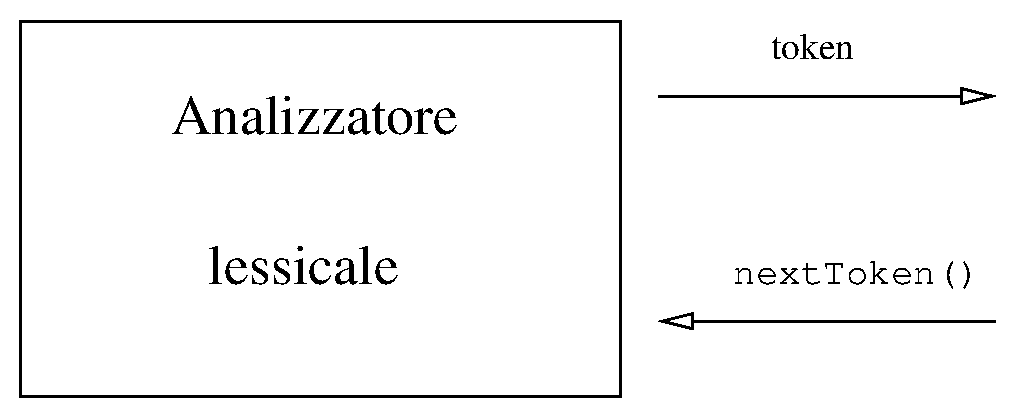
\epsfig{file = lexer.eps, width = 6cm}
\end{center}
\caption{L'interfaccia dell'analizzatore lessicale.}\label{fig:lexer}
\end{figure}
%
Il metodo \texttt{nextToken()} restituisce un token alla volta.

Genereremo l'analizzatore lessicale per Kitten in modo automatico, a partire
dalla specifica dei token che deve riconoscere. A tal fine useremo un
programma Java di nome JLex. La Figura~\ref{fig:jlex} mostra il
modo in cui generiamo l'analizzatore lessicale usando JLex.
%
\begin{figure}
\begin{center}
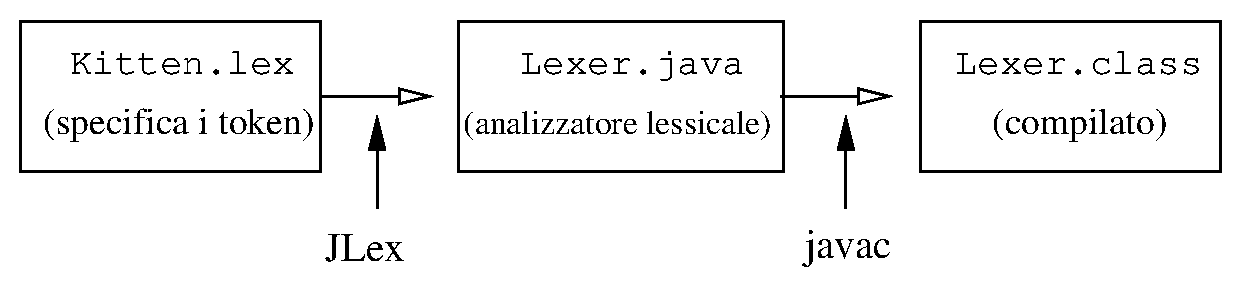
\epsfig{file = jlex.eps, width = \textwidth}
\end{center}
\caption{La generazione dell'analizzatore lessicale per Kitten.}
  \label{fig:jlex}
\end{figure}
%
Dentro al file \texttt{resources/Kitten.lex} enumeriamo
le espressioni regolari che denotano i token del linguaggio
Kitten, in una sintassi comprensibile dal programma JLex.
Per ogni espressione regolare va fornito, nel file
\texttt{resources/Kitten.lex}, un pezzo di codice
Java che viene eseguito quando viene riconosciuto il token corrispondente.
Normalmente tale codice Java non fa altro
che sintetizzare il token opportuno (\cioe un oggetto della classe
\texttt{java\_cup.runtime.Symbol} in Figura~\ref{fig:java_cup.runtime.Symbol})
e restituirlo.

Fornendo al programma JLex la specifica
\texttt{resources/Kitten.lex} dei token, otteniamo un programma Java
di nome \texttt{lexical/Lexer.java} che pu\`o essere compilato
come un qualsiasi programma Java. Tale programma \`e l'analizzatore
lessicale. Il nome \texttt{nextToken} della funzione che vogliamo generare
(Figura~\ref{fig:lexer}) viene specificato scrivendo la sua specifica dentro
\texttt{resources/Kitten.lex}:
%
\begin{verbatim}
%function nextToken
%type java_cup.runtime.Symbol
\end{verbatim}
%
con \texttt{\%type} abbiamo specificato il suo tipo di ritorno.

Programmi generati in maniera automatica, come \texttt{lexical/Lexer.java},
sono normalmente di difficile lettura per un essere umano.
Fidiamoci quindi del risultato e descriviamo invece in \piu dettagli
il contenuto del file \texttt{resources/Kitten.lex}.
%
\section{La specifica dei token}\label{sec:token_specification}
%
Abbiamo detto che il file \texttt{resources/Kitten.lex} contiene la
descrizione dei token Kitten, sotto forma di espressioni regolari con
associata un'azione di
sintesi del token corrispondente. Per esempio esso contiene le
seguenti coppie espressione regolare/azione:
%
\begin{verbatim}
  <YYINITIAL>while        {return tok(sym.WHILE, null);}
  <YYINITIAL>for          {return tok(sym.FOR, null);}
  ....
  <YYINITIAL>"+"          {return tok(sym.PLUS, null);}
  <YYINITIAL>"-"          {return tok(sym.MINUS, null);}
  <YYINITIAL>"*"          {return tok(sym.TIMES, null);}
  <YYINITIAL>"/"          {return tok(sym.DIVIDE, null);}
  <YYINITIAL>"="          {return tok(sym.EQ, null);}
  <YYINITIAL>"!="         {return tok(sym.NEQ, null);}
  <YYINITIAL>"<"          {return tok(sym.LT, null);}
  <YYINITIAL>"<="         {return tok(sym.LE, null);}
  ....
  <YYINITIAL>":="         {return tok(sym.ASSIGN, null);}
  ....
\end{verbatim}
%
che riconoscono rispettivamente
le parole chiave \texttt{while}, \texttt{for}, il segno di addizione ecc.
La sintassi \texttt{while} \`e un'espressione regolare che va intesa
come $\mathtt{w}\cdot\mathtt{h}\cdot\mathtt{i}\cdot\mathtt{l}\cdot\mathtt{e}$,
\cioe come la concatenazione sequenziale di cinque caratteri. La notazione
\texttt{<YYINITIAL>} specifica che queste regole sono attive quando
l'analizzatore lessicale \e nella \emph{modalit\`a} di default
\texttt{YYINITIAL}.
Parleremo \piu tardi delle modalit\`a (Sezione~\ref{sec:modes}).
Per adesso ci basta sapere che, all'inizio, l'analizzatore lessicale \e
in modalit\`a \texttt{YYINITIAL}, per cui le regole precedenti sono inizialmente attive.
L'azione corrispondente a ciascuna regola, che viene eseguita quando
il token corrispondente \`e stato riconosciuto, \`e fra parentesi graffe.
Si tratta di codice Java. Per adesso, esso sintetizza il token
corrispondente alle espressioni regolari, usando l'identificatore
numerico unico di ciascun token
(per esempio, \texttt{sym.WHILE}) e \texttt{null} come valore
lessicale. Il metodo \texttt{tok} non fa altro che costruire un oggetto
della classe in Figura~\ref{fig:java_cup.runtime.Symbol}:
%
\begin{verbatim}
private java_cup.runtime.Symbol tok(int kind, Object value) {
  return new java_cup.runtime.Symbol
    (kind, yychar, yychar + yylength(), value);
}
\end{verbatim}
%
La variabile \texttt{yychar} contiene il numero di caratteri tra l'inizio del
file e l'inizio del token. Il metodo \texttt{yylength()} ritorna
la lunghezza del token riconosciuto.
Metodi di ausilio, come quello precedente, sono inseriti in
\texttt{resources/Kitten.lex} fra i delimitatori \verb!%{! e
\verb!}%! e vengono ricopiati testualmente da JLex dentro
\texttt{lexical/Lexer.java}.

I token che hanno un valore lessicale sono specificati in maniera appena \piu
complicata:
%
\begin{verbatim}
<YYINITIAL>[a-zA-Z][a-zA-Z0-9_]*
    {return tok(sym.ID, yytext());}
<YYINITIAL>[0-9]+
    {return tok(sym.INTEGER, new Integer(yytext()));}
<YYINITIAL>[0-9]*"."[0-9]+
    {return tok(sym.FLOATING, new Float(yytext()));}
\end{verbatim}
%
Si noti come il valore lessicale degli identificatori \texttt{ID} sia
la stringa che rappresenta l'identificatore, mentre per interi e numeri
in virgola mobile si tratta, rispettivamente,
di un oggetto di classe \texttt{java.lang.Integer} e \texttt{java.lang.Float}.
Il programma JLex accorda maggiore priorit\`a alle regole
specificate prima in \texttt{resources/Kitten.lex}. Al fine, per esempio, di non
fare riconoscere la parola chiave \texttt{while} come un
identificatore, occorre mettere la regola per il \texttt{while}
prima di quella per gli identificatori (Sezione~\ref{sec:regular_expressions}).

Esiste infine una regola che riconosce qualsiasi carattere ma che, essendo
messa alla fine, viene eseguita solo quando nessun'altra regola
\`e applicabile. Tale regola segnala un errore lessicale, \cioe
la lettura di un carattere che non \e associabile ad alcun token:
%
\begin{verbatim}
  <YYINITIAL>.            {errorMsg.error(yychar, "Unmatched input");}
\end{verbatim}
%
Il carattere \texttt{.} (punto) \`e un'espressione regolare che denota
l'insieme dei caratteri dell'alfabeto. La si pu\`o immaginare come
un'abbreviazione dell'alternanza fra tutti i caratteri dell'alfabeto.
%
\javatip{
Se si dovessero aggiungere nuovi token all'enumerazione contenuta nel file
\texttt{resources/Kitten.lex}, occorrer\`a fare attenzione alla posizione in
cui le loro espressioni regolari vengono inserite. Molti studenti tendono
a inserire queste nuove espressioni regolari in fondo, dopo la regola
che usa il carattere punto. Questa \`e la peggior scelta che si pu\`o
fare: se il token \`e formato da un unico carattere, esso non verr\`a
mai riconosciuto perch\'e la regola col punto avr\`a priorit\`a sulla nuova
regola (Sezione~\ref{sec:regular_expressions}).
Se il token \`e formato da caratteri alfabetici, esso non
verr\`a mai riconosciuto perch\'e la regola per l'identificatore avr\`a
priorit\`a sulla nuova regola. \`E quindi consigliabile inserire le
espressioni regolari per nuovi token subito dopo l'enumerazione della
punteggiatura, prima degli identificatori.}
%
\section{La segnalazione di errori}\label{sec:errors}
%
Abbiamo appena visto che l'analizzatore lessicale pu\`o avere bisogno
di segnalare un errore all'utente di Kitten. Lo stesso (e molto \piu
spesso) accadr\`a con l'analizzatore sintattico e con quello semantico.
Tutti questi analizzatori usano la stessa classe
\texttt{errorMsg/ErrorMsg.java} per segnalare
errori. La sua interfaccia\footnote{
Per \piu informazioni sulle classi e i metodi di Kitten, ricordiamo
che \`e disponibile la documentazione JavaDoc dentro la
directory \texttt{javadoc} della distribuzione di Kitten.}
\e in Figura~\ref{fig:errorMsg.ErrorMsg}.
%
\begin{figure}[t]
\begin{verbatim}
public class ErrorMsg {
  /* costruttore: si chiede il nome del file che si sta compilando */
  public ErrorMsg(String fileName) { ... }

  /* chiamata quando si incontra un newline in fileName */
  public newline(int pos) { ... }

  /* segnala un errore msg alla posizione pos dall'inizio di fileName */
  public error(int pos, String msg) { ... }

  /* dice se si e' verificato almeno un errore */
  public boolean anyErrors() { ... }
}
\end{verbatim}
\caption{La classe \texttt{errorMsg.ErrorMsg.java} per la segnalazione di errori.}\label{fig:errorMsg.ErrorMsg}
\end{figure}
%
Il metodo \texttt{error()} segnala un errore all'utente. La posizione
dell'errore \e indicata all'utente con la notazione \texttt{riga:colonna}.
Ma il metodo \texttt{error()} richiede solo il numero \texttt{pos}
di caratteri passati dall'inizio del file che si sta compilando.
Per potere trasformare \texttt{pos} in \texttt{riga:colonna}, occorre
che l'oggetto di segnalazione di errori sia al corrente di dove, nel
file sorgente, si trovano i caratteri di newline. Ecco perch\'e, ogni volta
che si incontra tale carattere, l'analizzatore lessicale chiama il
metodo \texttt{newline()}:
%
\begin{verbatim}
  <YYINITIAL>\n           {errorMsg.newline(yychar);}
\end{verbatim}
%
Si noti che questa regola ha anche l'effetto secondario di
scartare il carattere newline, \poiche non vogliamo
i caratteri di spaziatura nel risultato dell'analisi lessicale
(Figura~\ref{fig:led_lexical}). Conoscendo le posizioni dei caratteri
di newline, \`e possibile sapere quanti newline occorrono nei primi
\texttt{pos} caratteri del file sorgente ed \`e quindi possibile
recuperare l'informazione di \texttt{riga}. La \texttt{colonna}
sar\`a il numero di caratteri tra l'ultimo newline e \texttt{pos}.

Il campo \texttt{errorMsg} dell'analizzatore lessicale
contiene la sua struttura di segnalazione di errore.
Essa \`e creata dal costruttore di
quest'ultimo a partire dal nome del file che si sta compilando.
%
\section{JLex: da espressioni regolari ad automi finiti non deterministici}
  \label{sec:nfa}
%
Abbiamo visto che JLex trasforma una sequenza di espressioni regolari
in un programma Java (l'analizzatore lessicale)
capace di riconoscere i token denotati da tali
espressioni regolari. Vediamo adesso di capire come funziona questo programma.

Le espressioni regolari sono degli ottimi strumenti per \emph{descrivere}
un insieme di stringhe, il loro linguaggio, ma certamente non per
\emph{riconoscere} tale insieme: data una stringa, vogliamo sapere se
appartiene o meno al linguaggio generato da una data espressione regolare.
Al fine di riconoscere un linguaggio, useremo degli \emph{automi a stati
finiti}, che ammettono una semplice implementazione algoritmica.
%
\begin{definition}[Automa Finito non Deterministico]\label{def:nfa}
Un \emph{automa finito non deterministico} su un alfabeto $\Lambda$ \`e un
grafo orientato finito i cui nodi sono detti \emph{stati} e i cui archi, detti
\emph{transizioni}, sono etichettati con un carattere in $\Lambda$ o con
$\varepsilon$. Un nodo del grafo \`e identificato come \emph{iniziale}
e un insieme di nodi del grafo come \emph{finali}.
\end{definition}
%
\begin{figure}[t]
\begin{center}
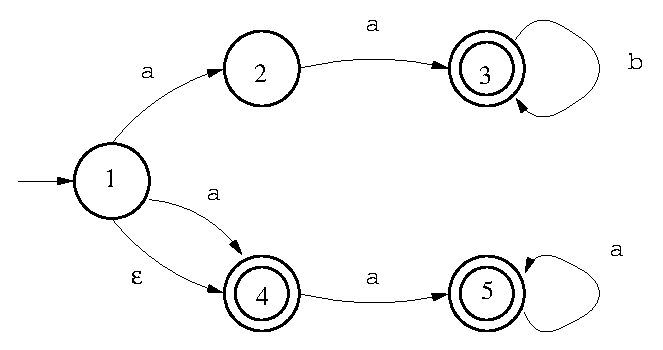
\epsfig{file = nfa.eps, width = 8cm}
\end{center}
\caption{Un automa finito non deterministico.}\label{fig:nfa}
\end{figure}
%
\noindent
La Figura~\ref{fig:nfa} mostra un automa finito non deterministico
sul linguaggio $\Lambda=\{\mathtt{a},\mathtt{b}\}$. Il nodo iniziale
\`e individuato da una freccia entrante. I nodi finali sono individuati
con una doppia cerchiatura.

Un \emph{percorso} in un automa \`e una sequenza di nodi legati da archi.
%
\begin{definition}[Percorso]\label{def:path}
Un \emph{percorso} in un automa finito non deterministico \`e una sequenza
di nodi $n_1\to^{c_1}n_2\to^{c_2}\cdots\to^{c_{k-1}}n_k$
tale che per ogni $i=1,\ldots,k-1$ esiste un arco $n_i\to^{c_i}n_{i+1}$
fra $n_i$ ed $n_{i+1}$. La \emph{stringa espressa} da un
percorso \`e la concatenazione delle etichette sugli archi che passano per i
nodi del percorso, cio\`e $c_1c_2\cdots c_{k-1}$.
\end{definition} 
%
\noindent
Per esempio, l'automa in Figura~\ref{fig:nfa} possiede un percorso
$4\to^\mathtt{a}5\to^\mathtt{a}5\to^\mathtt{a}5$ che esprime la stringa
\texttt{aaa}. Possiamo quindi definire il linguaggio \emph{accettato} da un
automa come l'insieme delle stringhe espresse da un percorso dell'automa
che comincia nel suo unico nodo iniziale e termina in un nodo finale.
%
\begin{definition}[Linguaggio Accettato da un Automa]\label{def:nfa_accept}
Il linguaggio $\mathcal{L}(A)$ \emph{accettato} da un automa non deterministico
$A$ \`e
\[
  \mathcal{L}(A)=\left\{s\in\Lambda^*\left|\begin{array}{l}
    s=c_1\cdots c_{k-1}\text{ ed esiste un percorso }n_1\to^{c_1}\cdots
      \to^{c_{k-1}}n_k\text{ di $A$}\\
    \text{tale che $n_1$ \`e il nodo iniziale di $A$ ed
          $n_k$ \`e un nodo finale di $A$}
  \end{array}\right.\right\}.
\]
\end{definition}
%
\noindent
Per esempio, possiamo determinare il linguaggio accettato dall'automa in
Figura~\ref{fig:nfa} considerando l'unione dei linguaggi accettati in ciascuno
dei suoi tre stati di accettazione. Essa \`e il linguaggio
fatto dalle stringhe che cominciano con due \texttt{a} e continuano con
un numero arbitrario (anche nullo) di \texttt{b}, dalle stringhe che
cominciano con una o due \texttt{a}
e continuano con un numero arbitrario (anche nullo)
di \texttt{a}, e dalla stringa vuota. Si noti che un automa pu\`o
accettare una stringa tramite vari percorsi differenti. Per esempio,
l'automa in Figura~\ref{fig:nfa} accetta la stringa \texttt{a} tramite
il percorso $1\to^\mathtt{a}4$ ma anche tramite il percorso
$1\to^\varepsilon 4\to^\mathtt{a}5$.

Il linguaggio accettato dall'automa in Figura~\ref{fig:nfa} \`e in effetti
quello denotato dall'espressione regolare $\varepsilon\mathtt{|aab^*
|aa^*|aaa^*}$ (che sarebbe possibile semplificare in $\mathtt{aab^*|a^*}$).
Questa non \`e una coincidenza: si pu\`o in effetti dimostrare
che, dato un linguaggio, esiste un automa finito non deterministico che
lo accetta se e solo se esiste un'espressione regolare che lo denota. Di questo
risultato vediamo adesso solo come \`e possibile costruire un automa finito non
deterministico a partire da una espressione regolare, in modo che quest'ultima
denoti lo stesso linguaggio accettato dall'automa. Pi\`u in dettaglio,
forniamo una definizione induttiva di un automa finito non deterministico
\emph{indotto} da una data espressione regolare.

Procediamo per induzione sulla struttura delle espressioni regolari, definendo
un automa non deterministico corrispondente a ciascun tipo di espressione
regolare della Definizione~\ref{def:regular_expression}. In questa costruzione
manterremo l'invariante che l'automa costruito avr\`a sempre
\emph{al pi\`u uno stato di accettazione}.

L'espressione regolare $\emptyset$ denota il linguaggio vuoto
(Definizione~\ref{def:regular_language}). Un automa che accetta lo
stesso linguaggio \`e il seguente:
%
\begin{center}
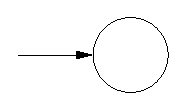
\epsfig{file = empty_nfa.eps, width = 3cm}
\end{center}
%
Esso non ha stati di accettazione e conseguentemente accetta
l'insieme vuoto di stringhe.

L'espressione regolare $\varepsilon$ denota un linguaggio che contiene la
sola stringa $\varepsilon$. Esso \`e lo stesso linguaggio accettato dall'automa
%
\begin{center}

\epsfig{file = epsilon_nfa.eps, width = 3cm}
\end{center}
%
Si noti che lo stato iniziale e quello di accettazione di questo automa
coincidono.

L'espressione regolare $a$, con $a\in\Lambda$, denota un linguaggio formato
dalla sola stringa $a$. Esso \`e lo stesso linguaggio accettato dall'automa
%
\begin{center}
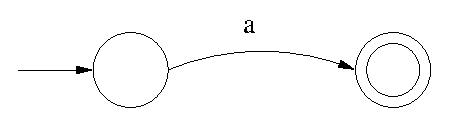
\epsfig{file = a_nfa.eps, width = 8cm}
\end{center}

L'espressione regolare $r_1r_2$, cio\`e la sequenza di due espressioni regolari
$r_1$ ed $r_2$, denota il linguaggio formato dalle stringhe ottenute
concatenando una stringa del linguaggio denotato da $r_1$ con una stringa
del linguaggio denotato da $r_2$. Otteniamo quindi un automa che accetta lo
stesso linguaggio concatenando sequenzialmente l'automa corrispondente ad
$r_1$ con l'automa corrispondente ad $r_2$:
%
\begin{center}
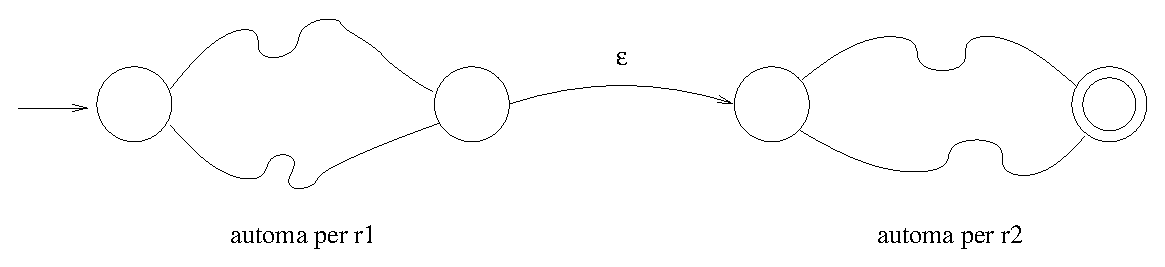
\epsfig{file = r1r2.eps, width = 15cm}
\end{center}
%
Si noti che lo stato di accettazione dell'automa corrispondente ad $r_1$
non \`e pi\`u di accettazione nell'automa composto per $r_1r_2$. Se inoltre
$r_1$ non ha stati di accettazione, allora la transizione etichettata con
$\varepsilon$ non viene aggiunta.

L'espressione regolare $r_1|r_2$ denota l'unione dei linguaggi di
$r_1$ e di $r_2$. Otteniamo quindi un automa che accetta lo stesso
linguaggio mettendo in alternativa gli automi corrispondenti alle
espressioni regolari $r_1$ ed $r_2$:
%
\begin{center}
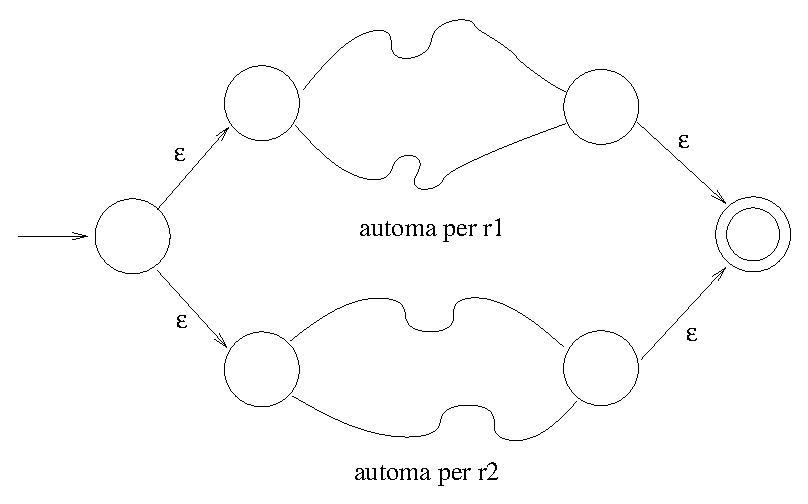
\epsfig{file = r1orr2.eps, width = 13cm}
\end{center}
%
Si noti che gli stati di accettazione degli automi corrispondenti ad $r_1$
ed $r_2$ non sono pi\`u di accettazione nell'automa composto per $r_1|r_2$,
mentre un nuovo stato di accettazione \`e stato aggiunto in quest'ultimo.
Se inoltre gli automi per $r_1$ o $r_2$ non hanno stati di accettazione
allora non si aggiunge la freccia (o le frecce) etichettate con
$\varepsilon$ che portano nello stato di accettazione.

L'espressione regolare $r^*$ denota il linguaggio ottenuto ripetendo un
numero arbitrario di volte le stringhe del linguaggio denotato da $r$.
Otteniamo un automa che accetta lo stesso linguaggio creando un ciclo
sull'automa corrispondente ad $r$. Questo ciclo pu\`o essere percorso
un numero arbitrario di volte, eventualmente anche nessuna volta:
%
\begin{center}
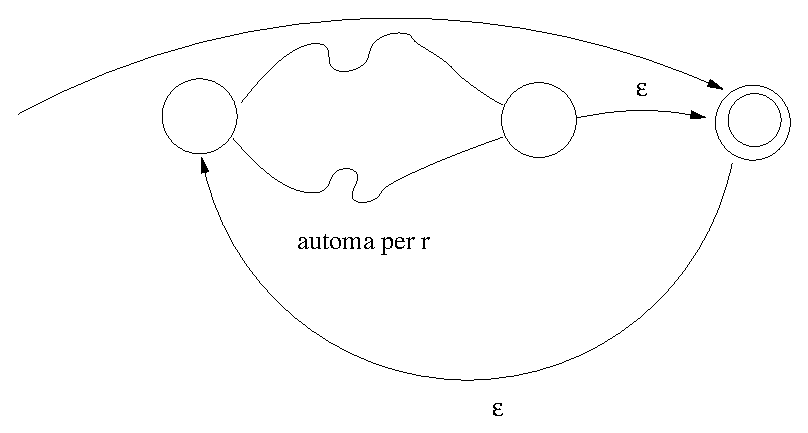
\epsfig{file = rstar.eps, width = 13cm}
\end{center}
%
Si noti che lo stato di accettazione dell'automa per $r$ non \`e pi\`u
di accettazione nell'automa per $r^*$ e che in quest'ultimo lo stato
finale e quello iniziale coincidono. Se inoltre l'automa corrispondente
ad $r$ non avesse alcuno stato di accettazione, non si metterebbe la transizione
etichettata con $\varepsilon$ che porta nello stato di accettazione.

Si consideri per esempio l'espressione regolare
$\mathtt{\varepsilon|aab^*|aa^*|aaa^*}$. Abbiamo gi\`a notato
che essa denota lo stesso linguaggio riconosciuto dall'automa
in Figura~\ref{fig:nfa}. Il risultato della costruzione esplicita di un automa
corrispondente a tale espressione regolare, usando le regole induttive di
costruzione che abbiamo appena descritto, \`e mostrato in
Figura~\ref{fig:nfa_built}.
%
\begin{figure}[t]
\begin{center}
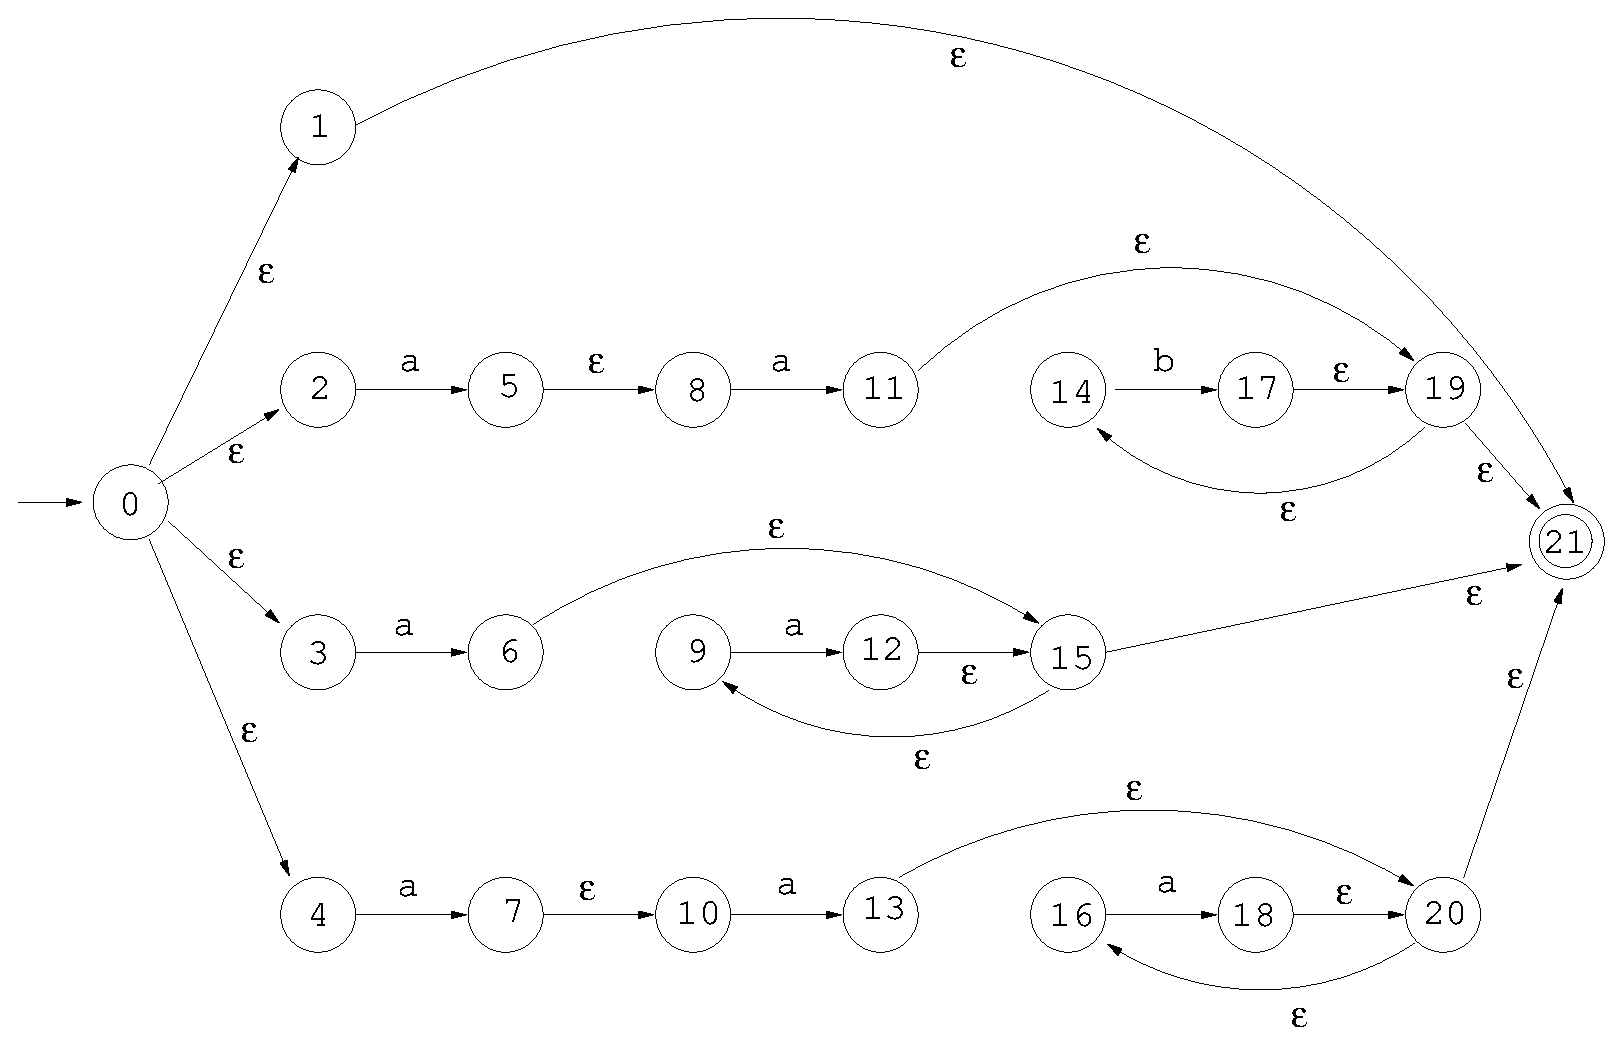
\epsfig{file = nfa_built.eps, width = 15cm}
\end{center}
\caption{Un automa finito non deterministico costruito induttivamente a partire dall'espressione regolare $\mathtt{\varepsilon|aab^*|aa^*|aaa^*}$. La numerazione dei nodi \`e arbitraria.}\label{fig:nfa_built}
\end{figure}
%
L'automa in Figura~\ref{fig:nfa_built} \`e diverso da quello in
Figura~\ref{fig:nfa}. In particolare, esso contiene \piu stati e transizioni.
I due automi sono per\`o \emph{equivalenti}, nel senso che essi
accettano lo stesso linguaggio (Definizione~\ref{def:nfa_accept}).
%
\section{JLex:
 da automi finiti non deterministici ad automi finiti deterministici}
  \label{sec:dfa}
%
La nozione di \emph{automa} che abbiamo dato nella Definizione~\ref{def:nfa}
caratterizza automi finiti \emph{non deterministici} in quanto \`e
possibile che ci siano \piu transizioni uscenti da uno stesso stato etichettate
con lo stesso carattere dell'alfabeto o transizioni etichettate con
$\varepsilon$. Se quindi tali automi sono utili
per \emph{descrivere} un linguaggio, essi sono per\`o scomodi per
\emph{riconoscere} un linguaggio, cio\`e per fornire una procedura effettiva
che permetta di determinare se una stringa appartiene o meno al linguaggio
che essi denotano. Occorrerebbe infatti a tal fine considerare tutti
i percorsi possibili nell'automa.

Se limitassimo ad al \piu uno il numero delle transizioni uscenti da uno
stesso stato etichettate con un dato carattere e vietassimo
delle transizioni etichettate con $\varepsilon$, otterremmo un tipo di automa
che ci permette di riconoscere se una stringa appartiene al linguaggio che
esso denota semplicemente cercando l'\emph{unico} percorso nell'automa
per tale stringa, se esiste. Questo nuovo tipo di automa \`e detto
\emph{deterministico}.
%
\begin{definition}[Automa Finito Deterministico]\label{def:dfa}
Un \emph{automa finito deterministico} \`e un automa finito
non deterministico senza transizioni etichettate con $\varepsilon$
e tale che per ciascun nodo e ciascun carattere
dell'alfabeto c'\`e al \piu una transizione
uscente dal nodo etichettata con tale carattere.
\end{definition}
%
\noindent
Per esempio, l'automa in Figura~\ref{fig:nfa} sarebbe deterministico se non
ci fosse la transizione etichettata con $\varepsilon$ e se le due
transizioni uscenti dal nodo $1$ ed etichettate con \texttt{a} avessero
etichette diverse.

Dal momento che un automa finito deterministico \`e un caso particolare
di automa finito non deterministico, le definizioni di \emph{percorso}
(Definizione~\ref{def:path}) e di \emph{linguaggio accettato}
(Definizione~\ref{def:nfa_accept}) sono valide anche per gli automi finiti
deterministici. \`E quindi immediato osservare che se un linguaggio \`e
accettato da un automa deterministico allora esso \`e accettato anche da un
automa non deterministico (lo stesso automa!). Il viceversa \`e anch'esso
vero, bench\'e meno immediato da dimostrare e intuitivamente meno ovvio.
In effetti \`e possibile simulare un automa finito non deterministico
con un automa deterministico i cui stati \emph{rappresentano} insiemi di
stati dell'automa non deterministico simulato. Questo significa che il
non determinismo non aggiunge potenza espressiva agli automi a stati finiti.

La trasformazione di un automa non deterministico in uno deterministico
comporta la definizione della \emph{$\varepsilon$-chiusura}
e della \emph{transizione su un carattere} di un insieme di stati.
%
\begin{definition}[$\varepsilon$-chiusura e transizione su un carattere]
  \label{def:closure}
Dato un automa finito non deterministico $A$ e un insieme $N$ dei suoi nodi,
la \emph{$\varepsilon$-chiusura} $\varepsilon(N)$ di $N$ \`e l'insieme $N$
stesso unito all'insieme dei nodi raggiungibili da un nodo di
$N$ usando solo transizioni etichettate con $\varepsilon$:
\[
  \varepsilon(N)=\{n'\in A\mid\text{esiste $n\in N$ tale che
                   $n\to^\varepsilon\cdots\to^\varepsilon n'$}\}.
\]
Se $c\in\Lambda$, la \emph{transizione su $c$ di $N$}, indicata come
$c(N)$, \`e l'insieme dei
nodi di $A$ raggiungibili da un nodo di $N$ tramite una transizione
etichettata con $c$ seguita da un numero arbitrario di transizioni
etichettate con $\varepsilon$:
\[
  c(N)=\varepsilon(\{n'\mid\text{esiste }n\in N\text{ tale che }
                   n\to^c n'\}).
\]
\end{definition}
%
\noindent
Per esempio, in Figura~\ref{fig:nfa_built} abbiamo
\begin{align*}
  \varepsilon(\{0\})&=\{0,1,2,3,4,21\}\\
  \varepsilon(\{5,8\})&=\{5,8\}\\
  \texttt{a}(\{0,1,2,3,4,21\})&=\{5,6,7,8,9,10,15,21\}\\
  \texttt{b}(\{0,1,2,3,4,21\})&=\emptyset.
\end{align*}

\`E possibile trasformare un automa finito non deterministico $A$ in uno
deterministico $A'$ equivalente i cui stati sono insiemi di stati di $A$.
Lo stato iniziale di $A'$ e $\varepsilon(i)$, dove $i$ \`e lo stato iniziale
di $A$. Da ogni stato $s$ di $A'$ e per ogni carettere $c$ dell'alfabeto,
esce da $s$ una transizione etichettata con $c$ che porta nello
stato $c(s)$ di $A'$. Se $c(s)=\emptyset$ allora si pu\`o fare a meno di
indicare la transizione. Gli stati di accettazione di $A'$ sono quelli che
contengono almeno uno degli stati di accettazione di $A$.
Per esempio, l'automa finito non deterministico in Figura~\ref{fig:nfa_built}
viene trasformato in quello deterministico mostrato in
Figura~\ref{fig:dfa_built}. Si noti che tutti i suoi stati sono di
accettazione.
%
\begin{figure}[t]
\begin{center}
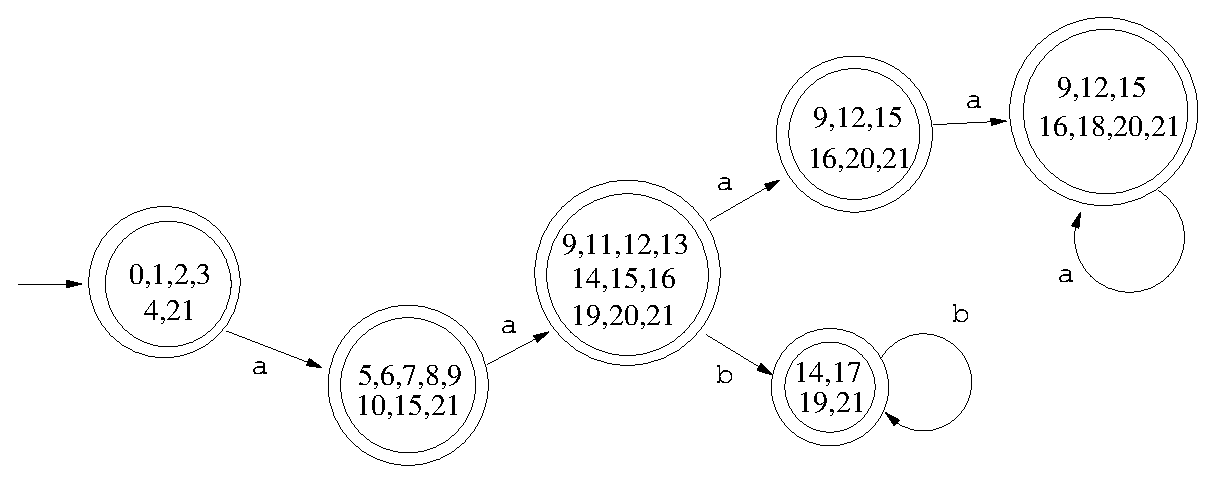
\epsfig{file = dfa_built.eps, width = 15cm}
\end{center}
\caption{Un automa finito deterministico ottenuto dall'automa non deterministico in Figura~\ref{fig:nfa_built}.}\label{fig:dfa_built}
\end{figure}

La trasformazione da espressione regolare ad automa della Sezione~\ref{sec:nfa}
fornisce in genere un automa finito \emph{non deterministico} a causa
delle regole di traduzione dell'alternanza di due espressioni regolari.
Tale automa pu\`o poi essere trasformato in un automa finito deterministico
equivalente con la trasformazione appena descritta. Questo \`e proprio
quello che fa JLex, ottenendo un automa deterministico che pu\`o
essere \piu comodamente eseguito su una macchina sequenziale.
Va detto comunque che, per maggiore efficienza, JLex
evita di costruire l'automa non deterministico ma costruisce invece
direttamente quello deterministico. Si tratta comunque di una ottimizzazione
della trasformazione fin qui descritta.

In genere l'automa ottenuto eliminando il
non determinismo potrebbe essere \emph{ridondante}, nel senso che
esso potrebbe contenere due stati con identiche funzioni, che possono quindi
venire fusi in un unico stato. Questo \`e per
esempio il caso degli stati $\{9,12,15,16,20,21\}$ e
$\{9,12,15,16,18,20,21\}$ in Figura~\ref{fig:dfa_built}. Essi potrebbero essere
fusi in un unico stato con una transizione uscente per \texttt{a} che porta
sullo stato stesso, riducendo il numero di stati dell'automa.
L'\emph{ottimizzazione} del numero di stati dell'automa deterministico
risultante dalla trasformazione viene quindi effettuata da JLex
al fine di ridurre la dimensione dell'automa deterministico finale.
Quest'ultimo viene infine scritto nel file \texttt{Lexer.java}
(Figura~\ref{fig:jlex}) sotto forma di un sorgente Java che contiene
l'insieme dei nodi e la tabella di transizione dell'automa.

Occorre adesso comprendere l'ultimo aspetto del funzionamento di JLex.
Esso infatti permette di riconoscere un \emph{insieme} di token e non una
sola espressione regolare. Inoltre esso implementa, fra tali token,
i meccanismi di coincidenza \piu lunga e priorit\`a delle regole
descritti nella Sezione~\ref{sec:regular_expressions}.
Consideriamo questi aspetti nella sezione seguente.
%
\section{JLex: la costruzione di un automa non deterministico per un insieme di token}\label{sec:jlex_for_tokens}
%
In Sezione~\ref{sec:nfa} abbiamo visto come un'espressione regolare possa
essere trasformata in un automa finito non deterministico che accetta lo
stesso linguaggio denotato dall'espressione regolare. In Sezione~\ref{sec:dfa}
abbiamo visto poi come tale automa possa venire trasformato in un automa
equivalente ma deterministico e quindi di \piu facile implementazione su una
macchina sequenziale. In questa sezione vediamo come JLex applica
queste tecniche per riconoscere un insieme di token.

JLex costruisce l'automa finito non deterministico corrispondente
all'espressione regolare che denota ciascun token, usando la tecnica
descritta nella Sezione~\ref{sec:nfa}. Tali automi vengono poi
messi in alternanza creando un unico, grande automa avente uno stato
iniziale legato agli stati iniziali di ciascun automa. Per esempio, per
i due token
%
\begin{verbatim}
  IF     if
  ID     [a-z][a-z]*
\end{verbatim}
%
il programma JLex costruisce l'automa
in Figura~\ref{fig:nfa_if_id}. Abbiamo etichettato alcune transizioni
con un intervallo di caratteri, il cui senso \`e che esse rappresentano in
effetti un \emph{insieme} di transizioni, una per ciascun carattere
nell'intervallo. Si noti inoltre che abbiamo annotato, accanto a
ciascuno stato di accettazione, qual \`e il token accettato in tale stato.
%
\begin{figure}[t]
\begin{center}
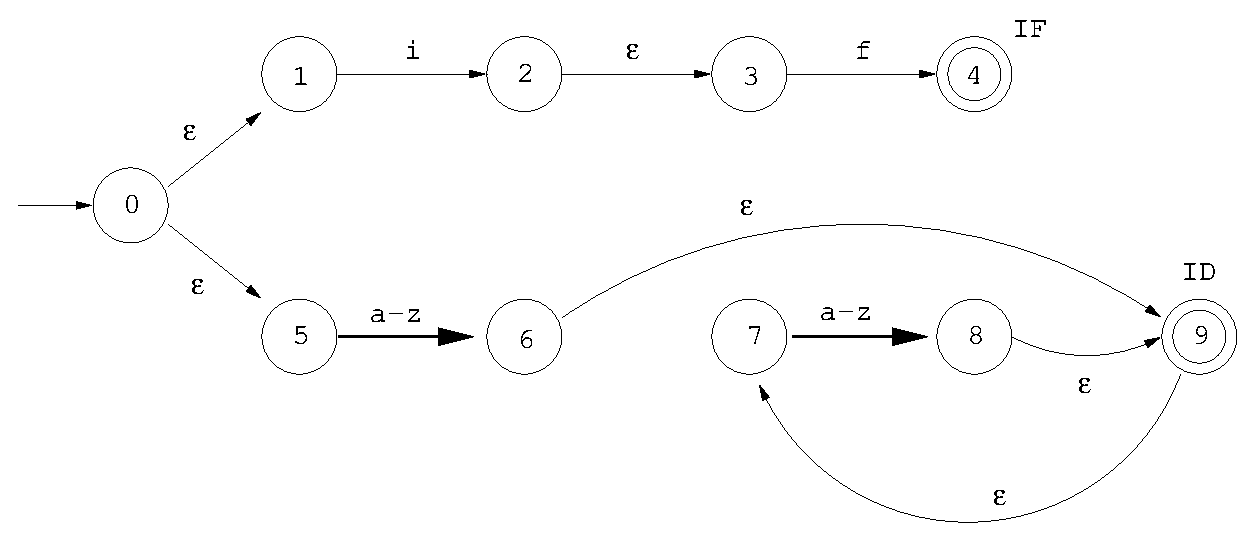
\epsfig{file = nfa_if_id.eps, width = 15cm}
\end{center}
\caption{Un automa finito non deterministico per i token \texttt{IF} ed \texttt{ID}.}\label{fig:nfa_if_id}
\end{figure}
%
JLex trasforma quindi tale automa in un automa finito deterministico,
con la tecnica descritta nella Sezione~\ref{sec:dfa}. Il risultato, per il
nostro esempio, \`e mostrato in Figura~\ref{fig:dfa_if_id}.
\`E possibile che uno stesso stato dell'automa deterministico venga etichettato
con \piu token, poich\'e contiene lo stato finale di \piu sotto-automi.
Questo \`e il caso dello stato etichettato con \texttt{IF} ed \texttt{ID}
in Figura~\ref{fig:dfa_if_id}. Questo significa che, se si arriva in tale stato,
allora i caratteri letti dall'inizio del file possono essere considerati sia
come un'istanza del token \texttt{ID} che come un'istanza del token
\texttt{IF}. Abbiamo gi\`a visto come si risolve questa ambiguit\`a:
dando precedenza al token che figura prima nell'enumerazione
(Sezione~\ref{sec:regular_expressions}).
Nel nostro caso, il token \texttt{IF} \`e stato enumerato per prima e
quindi l'etichetta \texttt{ID} viene rimossa e si decide che in tale stato si riconosce
solo il token \texttt{IF}.

Il risultato dell'elaborazione effettuata da JLex \`e quindi
un automa come quello in Figura~\ref{fig:dfa_if_id}, scritto in Java.
Ogni volta che si chiama il metodo \texttt{nextToken()}, tale automa viene
eseguito a partire dalla posizione corrente nel file sorgente. Quando occorre
fermarsi in questa lettura? Ci si potrebbe fermare non appena si finisce in uno
stato di accettazione. Ma questo significherebbe che \texttt{abc} verrebbe
riconosciuto come tre token \texttt{ID} piuttosto che come un unico token
\texttt{ID}. JLex decide quindi di avanzare nel file di input
finch\'e esiste una transizione possibile nell'automa. Quando non esiste
\piu alcuna transizione possibile, si restituisce il token che etichettava
l'ultimo stato di accettazione per cui si \`e passati.
Questo modo di procedere implementa quindi la \emph{coincidenza \piu
lunga} della Sezione~\ref{sec:regular_expressions}. Se nessuno stato di
accettazione \`e stato ancora incontrato, JLex
d\`a un messaggio di errore. Si noti comunque che quest'ultima situazione
\`e comunque impossibile nel caso di Kitten poich\'e nella enumerazione dei
token abbiamo inserito una regola di default che accetta qualsiasi carattere
(Sezione~\ref{sec:token_specification}).

L'implementazione dell'automa da parte di JLex deve tener conto di
un ultimo problema: i caratteri letti dopo l'ultimo stato di accettazione
per cui si \`e passati vanno \emph{rimessi} nel file di input per essere
processati alla prossima richiesta di \texttt{nextToken()}. A tal fine
basta utilizzare due puntatori nel file di input: uno che punta all'ultimo
stato di accettazione per cui si \`e passati e uno che punta all'ultimo
carattere letto. Prima di terminare una chiamata a \texttt{nextToken()},
JLex ha cura di riportare l'ultimo puntatore a coincidere col primo.
%
\begin{figure}[t]
\begin{center}
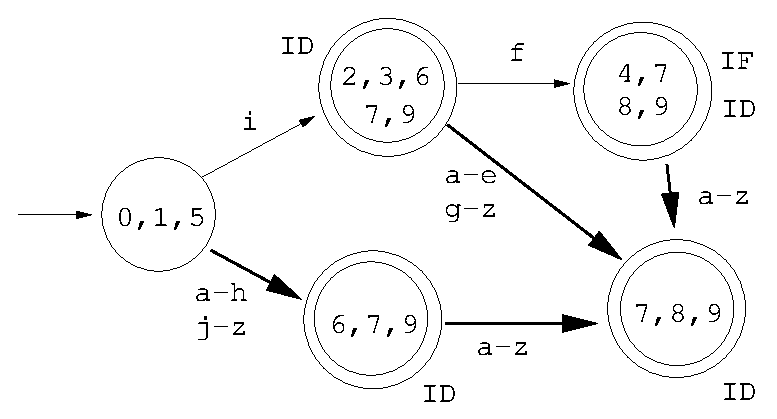
\epsfig{file = dfa_if_id.eps, width = 12cm}
\end{center}
\caption{L'automa finito deterministico costruito a partire dall'automa non deterministico in Figura~\ref{fig:nfa_if_id}.}\label{fig:dfa_if_id}
\end{figure}
%
\section{Modalit\`a lessicali: commenti e stringhe}\label{sec:modes}
%
Le regole contenute in \texttt{resources/Kitten.lex} hanno come
prefisso una \emph{modalit\`a} che indica quando esse sono attive. Normalmente,
l'analizzatore lessicale \`e nella modalit\`a di default \texttt{YYINITIAL}.
\`E possibile per\`o cambiare modalit\`a tramite il metodo
\texttt{yybegin()}. Occorre per prima cosa dichiarare le nuove modalit\`a
dentro \texttt{resources/Kitten.lex}:
%
\begin{verbatim}
  %state COMMENT
  %state STRING
\end{verbatim}
%
La scelta di queste due modalit\`a \`e finalizzata a semplificare la
gestione di commenti e stringhe. Per esempio,
la modalit\`a \texttt{COMMENT} si attiva quando incontriamo la sequenza
di caratteri \texttt{/*}:
%
\begin{verbatim}
  <YYINITIAL>"/*"         {commentCount++; yybegin(COMMENT);}
\end{verbatim}
%
La variabile \texttt{commentCount} conta il livello di annidamento
dei commenti visti fino a questo momento. Essa \e dichiarata fra i
delimitatori \verb!%{! e \verb!%}! e inizializzata a $0$.

Le uniche regole attive in modalit\`a \texttt{COMMENT} hanno come scopo
di scartare tutti i caratteri letti fino alla chiusura dell'ultimo
commento, tenendo conto dell'annidamento. Non dobbiamo per\`o dimenticare
di registrare le posizioni dei caratteri di newline:
%
\begin{verbatim}
  <COMMENT>"*/"           {commentCount--;
                           if (commentCount == 0) yybegin(YYINITIAL);}
  <COMMENT>"/*"           {commentCount++;}
  <COMMENT>\n             {newline();}
  <COMMENT>.              {}
\end{verbatim}

Occorre evitare che il file sorgente termini con un commento
ancora aperto. A tal fine usiamo il fatto che,
quando l'analizzatore lessicale giunge alla fine del file sorgente,
viene eseguito il codice specificato, dentro \texttt{resources/Kitten.lex},
fra i delimitatori \texttt{\%eofval\{} e \texttt{\%eofval\}}. Nel nostro
caso abbiamo scelto di eseguire quanto segue:
%
\begin{verbatim}
  %eofval{
          {
            if (commentCount != 0) err("Unclosed comment");
            return tok(sym.EOF, null);
          }
  %eofval}
\end{verbatim}
%
ovvero controlliamo che il file non termini con un commento ancora aperto e
poi restituiamo comunque il token fittizio \texttt{EOF}.

La modalit\`a \texttt{STRING} si attiva quando si incontra
un carattere di doppio apice. Essa riconosce la stringa fra doppi apici e
processa le sequenze di escape. Memorizza il valore lessicale dentro una
variabile \texttt{myString} che viene usata come valore lessicale del
token \texttt{STRING}:
%
\begin{verbatim}
  <YYINITIAL>"\"" {myString = ""; yybegin(STRING);}
  <STRING>\\n     {myString += "\n";}
  <STRING>\\t     {myString += "\t";}
  ... altre sequenze di escape ...
  <STRING>"\""    {yybegin(YYINITIAL); return tok(sym.STRING, myString);}
  <STRING>\n      {errorMsg.newline(yychar); myString += "\n";}
  <STRING>.       {myString += yytext();}
\end{verbatim}
%
La seconda e la terza regola inseriscono un carattere di escape
dentro la stringa quando viene riconosciuta la corrispondente
espressione di escape dentro il file sorgente. Si noti che l'espressione
regolare \verb!\\n! \`e formata da \emph{due} caratteri \verb!\\! e \texttt{n}.
Il primo \`e a sua volta una sequenza di escape di JLex per
esprimere il carattere \verb!\!. Esistono altre espressioni di escape
per inserire, per esempio, un carattere a partire dal suo codice ASCII.
Esse sono esaminabili dentro \texttt{resources/Kitten.lex}.
La terz'ultima regola riporta l'analizzatore in modalit\`a \texttt{YYINITIAL}
quando si incontra il carattere doppio apice di chiusura della stringa.
Le ultime due regole accumulano tutti caratteri dentro \texttt{myString}.
%
\greycomment{
L'uso di comandi Java con memoria, come l'assegnamento su \texttt{commentCount}
e \texttt{myString}, ha l'effetto di aumentare la potenza di JLex,
al punto che si potrebbe pensare di affidargli compiti molto \piu
complessi dell'analisi lessicale. Per esempio, la stessa analisi sintattica
(Capitolo~\ref{chap:syntactical})
potrebbe essere effettuata all'interno di JLex.
In effetti, l'uso di variabili Java d\`a a JLex la
capacit\`a di superare il potere espressivo limitato delle espressioni
regolari o degli automi a stati finiti, per accedere all'espressivit\`a
superiore di sistemi di riconoscimento di linguaggi basati su una quantit\`a di
memoria potenzialmente infinita, come gli automi a pila. Va per\`o
osservato che \`e \piu semplice
limitare l'uso di JLex allo scopo per cui
\`e stato pensato, cio\`e all'analisi lessicale, con qualche
\emph{concessione} all'uso di variabili Java per commenti e costanti
stringhe. Nel
Capitolo~\ref{chap:syntactical} useremo uno strumento \piu
adeguato, chiamato JavaCup,
per descrivere e riconoscere la struttura sintattica di Kitten.
}
%
\section{L'uso di JLex}\label{sec:use_jlex}
%
Una volta inserita dentro \texttt{resources/Kitten.lex} la specifica
dell'analizzatore lessicale che vogliamo generare, non ci rimane
che generarlo tramite JLex. A tal fine basta eseguire un piccolo programma
Java che chiama la classe di generazione dell'analizzatore lessicale
fornita nel jar di JLex, specificando dov'\`e la specifica dei token e qual \`e
il nome dell'analizzatore lessicale Java da generare:
%
\begin{verbatim}
public class Generator {
  public static void main(String[] args) throws IOException {
    new CLexGen("resources/Kitten.lex", "src/lexical/Lexer").generate();
  }
}
\end{verbatim}
%
Baster\`a quindi eseguire tale programma Java per generare \texttt{lexical/Lexer.java}
dentro la directory \texttt{src}. Avremo in effetti ottenuto un analizzatore lessicale
\texttt{lexical/Lexer.java} che contiene un costruttore
%
\begin{verbatim}
  public Lexer(fileName)
\end{verbatim}
%
e un metodo
%
\begin{verbatim}
  public java_cup.runtime.Symbol nextToken()
\end{verbatim}
%
che estrae e restituisce un token alla volta da \texttt{fileName} (Figura~\ref{fig:lexer}).
Per comodit\`a, l'esecuzione
di tale programma di generazione dell'analizzatore lessicale \e automatizzata
tramite il task Ant \texttt{generate-lexical-analyzer}.

Il passo successivo \e a questo punto quello di compilare
anche \texttt{lexical/Lexer.java}.
Anche questo processo \e stato automatizzato nel task Ant
\texttt{compile-lexical-analyzer}. Infine, possiamo usare l'analizzatore lessicale
per effettuare l'analisi lessicale di un sorgente Kitten.
Questo viene effettuato dal programma Java \texttt{lexical/Main.java},
che prima istanzia l'analizzatore lessicale:
%
\begin{verbatim}
  Lexer lexer = new Lexer(fileName);
\end{verbatim}
%
e poi chiama ripetutamente \texttt{lexer.nextToken()} in un ciclo, finch\'e non viene letto
il token \texttt{EOF}. La compilazione di tale programma e la sua invocazione sul sorgente Kitten
specificato dentro \verb|build.properties| sono state automatizzate con il task Ant
\texttt{run-lexical-analyzer}.
%
\begin{exercise}\label{ex:regular_odd}
Si consideri il linguaggio $\Lambda=\{\mathtt{0},\mathtt{1}\}$.
Si definisca un'espressione regolare che denota tutti e soli i numeri binari
dispari.
\end{exercise}
%
\begin{exercise}\label{ex:r1r2}
In Sezione~\ref{sec:nfa} abbiamo trasformato la sequenza $r_1r_2$ di
due espressioni regolari $r_1$ ed $r_2$ in un automa ottenuto
legando gli automi ottenuti per $r_1$ ed $r_2$, rispettivamente,
con una transizione etichettata con $\varepsilon$. Si provi
a giustificare perch\'e tale transizione \`e necessaria e non
pu\`o invece essere eliminata fondendo lo stato finale
dell'automa per $r_1$ con lo stato iniziale dell'automa per $r_2$.
\end{exercise}
%
\begin{exercise}\label{ex:rstar}
In Sezione~\ref{sec:nfa} abbiamo trasformato l'iterazione $r^*$ di
un'espressione regolare $r$ in un automa ottenuto a partire dall'automa
per $r$. Abbiamo per\`o aggiunto un nuovo stato terminale e, al contempo,
iniziale. Si provi a giustificare perch\'e tale stato \`e necessario e non
\`e possibile invece usare come stato iniziale e terminale
lo stato finale dell'automa per $r$.
\end{exercise}
%
\begin{exercise}\label{ex:nfa}
Si definisca, usando le tecniche descritte in questo capitolo,
un automa non deterministico che accetta i token
\texttt{CONST}, \texttt{CONTINUE} ed \texttt{ID}.
\end{exercise}
%
\begin{exercise}\label{ex:dfa_three}
Si consideri il linguaggio delle cifre decimali. Si definisca un'automa finito
deterministico che accetta tutti i soli i numeri decimali divisibili per $3$.
\end{exercise}
%
\begin{exercise}\label{ex:nfatodfa}
Si trasformi l'automa non deterministico dell'esercizio~\ref{ex:nfa}
in un automa finito deterministico.
\end{exercise}

\chapter{Analisi Sintattica}\label{chap:syntactical}
%
\vspace*{-2ex}
\begin{center}
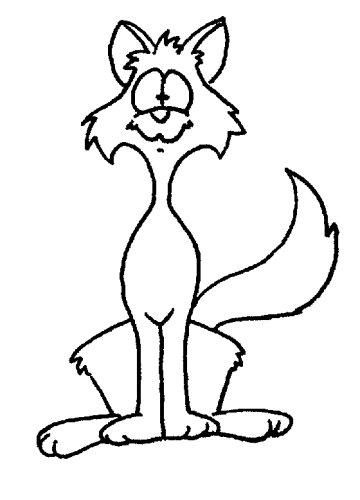
\includegraphics[width=6cm]{cat2.jpeg}
\end{center}
\vspace*{-2ex}
%
Nel Capitolo~\ref{chap:lexical} abbiamo visto come la sequenza di
caratteri di un sorgente Kitten possa venire trasformata in una lista
di \emph{token}. Programmi \emph{lessicalmente errati}, \cioe
contenenti sequenze di caratteri che non compongono alcun
token, vengono rifiutati dall'analizzatore lessicale con una segnalazione
di errore.

Questo non significa per\`o che l'analizzatore lessicale impedisca
al programmatore di scrivere programmi \emph{sintatticamente errati}.
Per esempio, il comando
\[
  \verb|while (a != b a := a + 1|
\]
viene tradotto nella sequenza di token \texttt{WHILE}, \texttt{LPAREN},
\texttt{ID}, \texttt{NEQ}, \texttt{ID}, \texttt{ID}, \texttt{ASSIGN},
\texttt{ID}, \texttt{PLUS}, \texttt{INTEGER} senza che alcun messaggio
di errore venga segnalato dall'analizzatore lessicale. Ci\`o nonostante,
tale comando \`e sintatticamente errato in quanto contiene una parentesi
tonda aperta che non \`e stata richiusa. In questo capitolo intendiamo
presentare delle tecniche che permettono di segnalare al programmatore
errori sintattici come quello appena mostrato. Tali tecniche sono
chiamate tecniche di analisi sintattica o di \emph{parsing}.
L'analisi sintattica ha due scopi:
%
\begin{itemize}
\item garantire
  che il codice rispetti le regole sintattiche del linguaggio. Se \cosi non
  \`e, un errore di sintassi deve essere segnalato al programmatore;
\item costruire una rappresentazione
  \emph{strutturata} del programma, detta \emph{sintassi astratta} del
  programma, che pu\`o essere \emph{comodamente}
  usata dalle successive fasi di analisi semantica e di generazione e
  ottimizzazione del codice.
\end{itemize}
%
\begin{figure}
\begin{center}
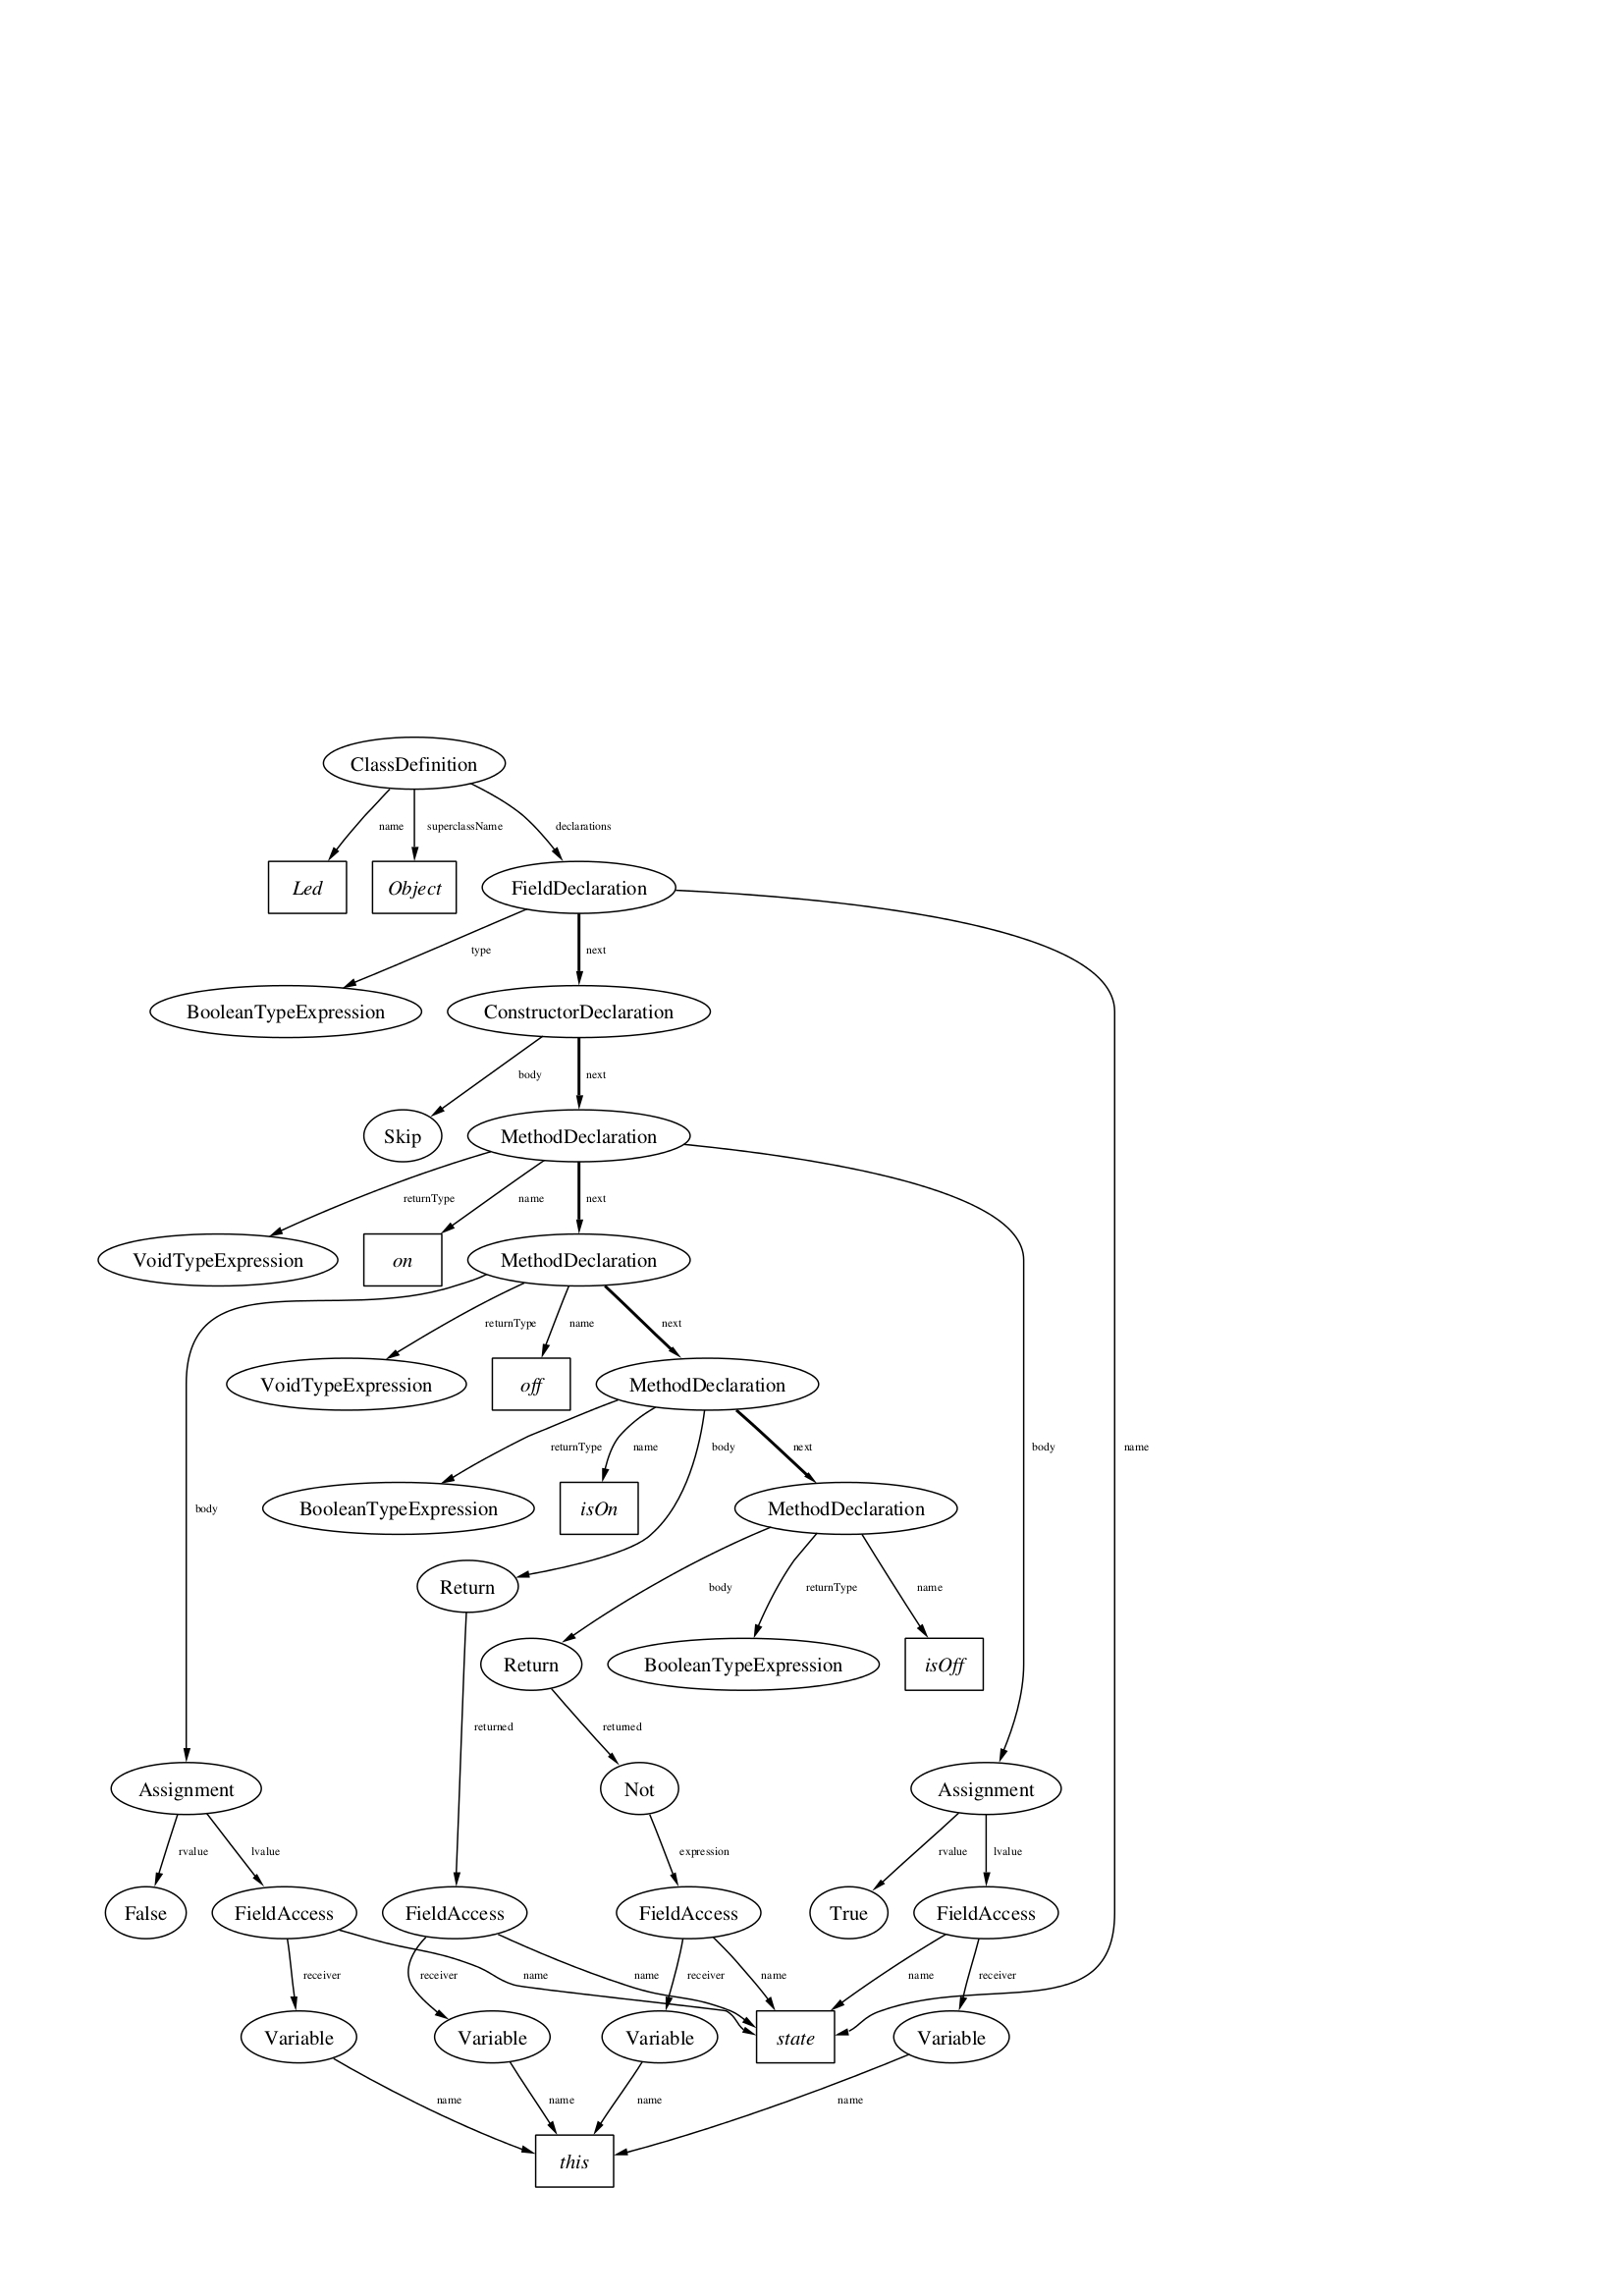
\includegraphics[width=16cm]{led_logica.jpg}
\end{center}
\caption{La sintassi astratta del programma in Figura~\ref{fig:led}.}
  \label{fig:led_albero}
\end{figure}
%
Si consideri per esempio il programma in Figura~\ref{fig:led}. L'analisi
sintattica di Kitten accetta tale programma come sintatticamente corretto
e genera la sua struttura logica mostrata in Figura~\ref{fig:led_albero}.
Tale struttura logica \`e chiamata \emph{albero di sintassi astratta}
del programma la cui \emph{sintassi concreta} \`e in Figura~\ref{fig:led}.
Vedremo in futuro (Sezione~\ref{sec:abstract_syntax_classes})
come interpretare i nodi di questo albero. Per adesso
osserviamo solo che i nodi ovali rappresentano categorie di sintassi
astratta composte a partire dai sottoalberi ivi radicati. I nodi rettangolari
sono invece gli identificatori del programma e sono condivisi quando
occorrono pi\`u volte nel codice. In effetti, quindi, sarebbe pi\`u
corretto parlare di \emph{grafo} di sintassi astratta. Preferiamo comunque
continuare a chiamarlo albero dal momento che almeno
i nodi ovali sono raggiungibili tramite
un unico percorso a partire dalla radice dell'albero (posta in alto).
L'albero in Figura~\ref{fig:led_albero} \`e \piu \emph{comodo} da
maneggiare da parte di un computer che una sequenza di caratteri come
quella in Figura~\ref{fig:led}. Esso infatti \`e una vera e propria
struttura dati i cui diversi livelli di profondit\`a esprimono
la struttura del codice sorgente. Questa struttura \`e invece
meno evidente nel codice sorgente.

In questo capitolo parleremo, nell'ordine, delle \emph{grammatiche libere
dal contesto} (Sezione~\ref{sec:grammar}), che sono lo strumento che useremo
per descrivere la sintassi del codice sorgente di un programma.
Passeremo quindi a descrivere l'uso di uno strumento,
chiamato JavaCup, che permette di creare automaticamente
un analizzatore sintattico a partire dalla grammatica del linguaggio
che esso deve riconoscere (Sezione~\ref{sec:java_cup}).
Quindi analizzeremo il funzionamento di JavaCup, partendo
da un modo semplice ma poco potente di effettuare il parsing
(Sezione~\ref{sec:ll}) e passando quindi a una tecnica \piu
potente (Sezione~\ref{sec:lr}). Infine descriveremo la costruzione
dell'albero di sintassi astratta da parte di JavaCup
(Sezione~\ref{sec:abstract_syntax}) e la struttura dell'albero
di sintassi astratta stesso (Sezione~\ref{sec:abstract_syntax_classes}).
%
\section{Le grammatiche libere dal contesto}\label{sec:grammar}
%
La potenza delle espressioni regolari \`e limitata poich\'e esse
corrispondono a uno strumento di calcolo con una quantit\`a di memoria
limitata a priori (gli \emph{automi a stati finiti} della
Sezione~\ref{sec:nfa}). Esse non sono quindi in grado di esprimere
linguaggi la cui definizione richiede la capacit\`a di \emph{contare}
fino a livelli di profondit\`a arbitrari, come per esempio il linguaggio
%
\[
  P=\{\mathtt{a}^n\mathtt{b}^n\mid n\ge 0\}.
\]
Visto il primo carattere \texttt{b}, occorre ricordarsi quanti caratteri
\texttt{a} si sono visti per sapere quanti caratteri \texttt{b}
ci si deve ancora aspettare. Il \emph{linguaggio di parentesi} $P$ non \`e
un puro gioco teorico: esso astrae un tipico linguaggio di programmazione
la cui struttura \`e data da delimitatori come le parentesi graffe
o le parole chiave \texttt{begin} ed \texttt{end}, che devono essere
accoppiati: ad ogni apertura deve corrispondere una chiusura.

Abbiamo visto nella Sezione~\ref{sec:modes} che le espressioni regolari
posso essere \emph{potenziate} utilizzando delle \emph{azioni con memoria}
(come l'assegnamento). Ma si tratta di una trucco scomodo per descrivere
la complessa sintassi di un linguaggio di programmazione. Meglio \`e invece
identificare uno strumento di descrizione di linguaggi strettamente \piu
potente delle espressioni regolari e naturalmente portato a descrivere la
sintassi dei linguaggi di programmazione. Questo strumento sono le
\emph{grammatiche libere dal contesto}.
%
\begin{definition}[Grammatica Libera dal Contesto]\label{def:grammar}
Una \emph{grammatica libera dal contesto} (in seguito semplicemente
\emph{grammatica}) su un alfabeto $\Lambda$
\`e una quadrupla $\langle T,N,I,P\rangle$ dove
\begin{itemize}
\item $T\subseteq\Lambda$
      \`e un insieme detto dei \emph{simboli terminali} o semplicemente
      dei \emph{terminali}
\item $N$ \`e un insieme
      detto dei \emph{simboli non terminali} o semplicemente
      dei \emph{non terminali}
\item $I\in N$ \`e il \emph{non terminale iniziale}
\item $P$ \`e un insieme di \emph{produzioni}, \cioe di frecce del tipo
      $L\to\gamma$ dove $L\in N$ \`e il \emph{lato sinistro} della produzione
      e $\gamma\in (T\cup N)^*$ \`e una sequenza anche vuota di terminali e
      non terminali, detta \emph{lato destro} della produzione.
\end{itemize}
%
Indicheremo in grassetto i terminali, in italico
i non terminali e con lettere greche le sequenze, possibilmente vuote,
di terminali e non terminali, dette anche \emph{forme sentenziali}.
La forma sentenziale vuota sar\`a sempre indicata come $\varepsilon$. Si noti
che il lato destro di una produzione \`e una forma sentenziale.
Una forma sentenziale \`e detta \emph{ground} o \emph{stringa}
se non contiene non terminali.
\end{definition}

Un esempio di grammatica \`e la quadrupla $\langle T,N,I,P\rangle$ dove
%
\begin{equation}\label{eq:example_grammar}
\begin{split}
  T &= \{\mathtt{a},\mathtt{b}\}\\
  N &= \{I\}\\
  P &= \{I\to\varepsilon,\ I\to\mathtt{a}I\mathtt{b}\}.
\end{split}
\end{equation}
%
Essa \`e una grammatica per qualsiasi linguaggio che contenga almeno i simboli
$\mathtt{a}$ e $\mathtt{b}$. In futuro descriveremo una grammatica
semplicemente enumerando le sue produzioni. Assumeremo implicitamente
che $T$ \`e l'insieme dei terminali che occorrono nelle produzioni enumerate
e che $N$ \`e l'insieme dei non terminali che occorrono nelle produzioni
enumerate. Assumeremo inoltre che $I$ sia il non terminale a sinistra della
prima produzione.
%
\begin{definition}[Derivazione]\label{def:derivation}
Data una grammatica $G=\langle T,N,I,P\rangle$ e due forme sentenziali
$\alpha$ e $\beta$, diciamo che $\beta$ \`e
\emph{derivabile in $G$ in un passo}
da $\alpha$ se e solo se esiste una produzione
$L\to\gamma\in P$ tale che $\alpha=\eta L\delta$ e $\beta=\eta\gamma\delta$.
In tal caso scriveremo che $\alpha\Rightarrow_G\beta$.
Una \emph{derivazione} per $G$ \`e la concatenazione di pi\`u passi
di derivazione $\alpha\Rightarrow\beta_1\Rightarrow\beta_2\ldots$
Indicheremo con
$\Rightarrow^*_G$ la chiusura riflessiva e transitiva di $\Rightarrow$.
Quando $G$ \`e chiara dal contesto, eviteremo di indicarla esplicitamente
nelle notazioni $\Rightarrow$ e $\Rightarrow^*$.
\end{definition}
%
\noindent
Per esempio, nella grammatica~\eqref{eq:example_grammar} si ha
%
\begin{align*}
  \mathtt{ab}I\mathtt{b}&\Rightarrow\mathtt{aba}I\mathtt{bb}\\
  \mathtt{aba}I\mathtt{bb}&\Rightarrow\mathtt{ababb}\\
  I&\Rightarrow\mathtt{a}I\mathtt{b}\\
  I&\Rightarrow^*I\\
  \mathtt{ab}I\mathtt{b}&\Rightarrow^*\mathtt{ababb}.
\end{align*}

Le grammatiche servono a descrivere linguaggi, esattamente come gli automi a
stati finiti. In particolare, una grammatica genera il linguaggio formato
dalle stringhe derivabili dal non terminale iniziale.
%
\begin{definition}[Linguaggio generato da una grammatica]
  \label{def:gen_grammar}
Data una grammatica $G$ su un alfabeto $\Lambda$,
il linguaggio $L(G)$ da essa generato \`e
\[
  L(G)=\{\alpha\text{ ground}\mid I\Rightarrow^*\alpha\}.
\]
\end{definition}
%
\noindent
Per esempio, il linguaggio generato dalla grammatica~\eqref{eq:example_grammar}
\`e
%
\[
  L(G)=\{\mathtt{a}^n\mathtt{b}^n\mid n\ge 0\}=P.
\]
%
Questo mostra che le grammatiche libere dal contesto permettono di generare
linguaggi, come $P$, che non possono essere generati con automi a stati finiti.
Pi\`u in generale, si pu\`o
mostrare che ogni linguaggio generabile da un automa a stati
finiti \`e anche generabile da una grammatica libera dal contesto.
Conseguentemente, le grammatiche descrivono strettamente
pi\`u linguaggi che gli automi a stati finiti.

Data una forma sentenziale $\alpha$, potrebbe esserci pi\`u di un
$\beta$ tale che $\alpha\Rightarrow\beta$. Per esempio, nella
grammatica~\eqref{eq:example_grammar} abbiamo
$I\mathtt{b}\Rightarrow\mathtt{b}$
ma anche $I\mathtt{b}\Rightarrow\mathtt{a}I\mathtt{bb}$.
In questo caso abbiamo la possibilit\`a di scegliere quale produzione
usare per sostituire lo stesso non terminale $I$. In altri casi la
pluralit\`a delle scelte \`e la conseguenza di pi\`u occorrenze
di non terminali in $\alpha$. Si consideri per esempio la grammatica
%
\begin{equation}\label{eq:other_grammar}
\begin{split}
  I&\to\varepsilon\\
  I&\to\mathtt{a}\\
  I&\to\mathtt{b}\\
  I&\to II
\end{split}
\end{equation}
%
(come detto sopra, l'enumerazione delle produzioni \`e sufficiente
a definire la grammatica). La stessa stringa
$\mathtt{abb}$ possiamo derivarla tramite le derivazioni:
%
\begin{figure}[t]
\[
\xymatrix{
  & I\ar[ld]\ar[d]\ar[rd] \\
\mathtt{a} & I\ar[ld]\ar[d]\ar[rd] & \mathtt{b}\\
\mathtt{a} & I\ar[d] & \mathtt{b}\\
  & \varepsilon
}
\]
\caption{Un albero di derivazione per la
         grammatica~\eqref{eq:example_grammar}.}\label{fig:parse_tree}
\end{figure}
%
\begin{equation}\label{eq:many_derivations}
\begin{split}
  I&\Rightarrow II\Rightarrow I\mathtt{b}\Rightarrow II\mathtt{b}
    \Rightarrow\mathtt{a}I\mathtt{b}\Rightarrow\mathtt{abb}\\
  I&\Rightarrow II\Rightarrow III\Rightarrow II\mathtt{b}
    \Rightarrow\mathtt{a}I\mathtt{b}\Rightarrow\mathtt{abb}\\
  I&\Rightarrow II\Rightarrow I\mathtt{b}\Rightarrow II\mathtt{b}
    \Rightarrow I\mathtt{bb}\Rightarrow\mathtt{abb}.
\end{split}
\end{equation}
%
In questo caso la scelta riguarda l'ordine col quale sostituiamo le $I$.
Va osservato che questo secondo tipo di \emph{libert\`a di scelta} \`e
in effetti irrilevante, nel senso che, qualsiasi scelta si faccia, \`e poi
possibile effettuare un'altra sostituzione, temporaneamente
ritardata. Questa caratteristica delle grammatiche libere dal contesto dice
essenzialmente che il criterio con cui si sostituiscono i non terminali
in una forma sentenziale non cambia l'insieme delle stringhe
derivabili. Potremmo per esempio scegliere indifferentemente
di sostituire sempre prima
i non terminali pi\`u a sinistra (derivazioni \emph{leftmost}) o prima
quelli pi\`u a destra (derivazioni \emph{rightmost}).

Un modo per astrarre dall'ordine delle sostituzioni \`e quello di usare
degli \emph{alberi di parsing} al posto delle derivazioni stesse. Un albero
di parsing rappresenta un \emph{insieme} di derivazioni, tutte quelle
che derivano la stessa stringa, a partire dal non terminale
di partenza, con qualsiasi criterio di sostituzione.
%
\begin{definition}[Albero di parsing o di derivazione]\label{def:parsing_tree}
Un \emph{albero di parsing} o \emph{di derivazione}
per una grammatica $G=\langle T,N,I,P\rangle$ \`e un albero tale che:
\begin{enumerate}
\item i suoi nodi sono etichettati con un elemento di $N$ o di $T$ o con $\varepsilon$
\item la radice \`e etichettata con $I$
\item le foglie sono etichettate con elementi di $T$ o con $\varepsilon$
\item dato un nodo etichettato come $L$ e prese, da sinistra a destra,
      le etichette $e_1,\ldots,e_n$ dei suoi figli, allora
      $L\to e_1\cdots e_n\in P$.
\end{enumerate}
La concatenazione delle etichette della
frontiera dell'albero, letta da sinistra a destra secondo una visita
leftmost in profondit\`a, \`e la stringa
\emph{derivata} dall'albero a partire dalla sua radice.
\end{definition}
%
\noindent
Per esempio, la Figura~\ref{fig:parse_tree} mostra un albero di derivazione
per la grammatica~\eqref{eq:example_grammar}. Esso deriva la stringa
$\mathtt{aabb}$ e astrae l'insieme di derivazioni
\[
  \{I\Rightarrow\mathtt{a}I\mathtt{b}\Rightarrow\mathtt{aa}I\mathtt{bb}
    \Rightarrow\mathtt{aabb}\}.
\]
%
L'albero a sinistra nella Figura~\ref{fig:ambiguity} \`e un albero di
derivazione per la grammatica~\eqref{eq:other_grammar}. Esso deriva la stringa
$\mathtt{abb}$ e astrae un insieme di derivazioni che include, fra
le altre, le derivazioni~\eqref{eq:many_derivations}.

Gli alberi di derivazione rappresentano insiemi di derivazioni che possiamo
considerare equivalenti e interscambiabili. In particolare,
un albero di derivazione
specifica la struttura logica delle derivazioni che esso rappresenta:
come cio\`e la stringa sulla sua frontiera viene costruita
a partire dal non terminale iniziale, senza entrare nei dettagli dell'ordine
con cui questa costruzione \`e effettuata. Ne consegue che, se una stessa
stringa $\alpha$ ammette due alberi di derivazione diversi, allora
ci sono almeno due modi, \emph{strutturalmente diversi}, di derivare $\alpha$.
%
\begin{figure}[t]
\[
\xymatrix{
   &   & I\ar[ld]\ar[rd] \\
   & I\ar[ld]\ar[rd] &   & I\ar[d]\\
 I\ar[d] &   & I\ar[d] & \mathtt{b}\\
 \mathtt{a} & & \mathtt{b}
}
\qquad\qquad\qquad
\xymatrix{
  & I\ar[ld]\ar[rd] \\
I\ar[d] &   & I\ar[ld]\ar[rd]\\
\mathtt{a} & I\ar[d] &  & I\ar[d]\\
  & \mathtt{b} &  & \mathtt{b}
}
\]
\caption{Due alberi di derivazione diversi per la stessa stringa $\mathtt{abb}$.}\label{fig:ambiguity}
\end{figure}
%
\begin{definition}[Grammatica ambigua]\label{def:ambiguity}
Una grammatica $G$ \`e \emph{ambigua} se e solo se esiste una forma
sentenziale ground $\alpha$ che ammette due alberi di parsing diversi in $G$.
\end{definition}
%
\noindent
Per esempio, la grammatica~\eqref{eq:other_grammar} \`e ambigua poich\'e
ammette due alberi di derivazione diversi per la stringa
$\mathtt{abb}$, come mostrato in Figura~\ref{fig:ambiguity}.

Le grammatiche ambigue ci porranno dei problemi poich\'e non specificano
un'unica struttura per le stringhe di un linguaggio, ma danno la
possibilit\`a di interpretarle strutturalmente in modo diverso. Per esempio,
la Figura~\ref{fig:ambiguity} mostra che la stringa $\mathtt{abb}$ pu\`o
essere interpretata nella grammatica~\eqref{eq:other_grammar}
come la stringa $\mathtt{ab}$ seguita da una
$\mathtt{b}$ (albero a sinistra)
o come una $\mathtt{a}$ seguita dalla stringa $\mathtt{bb}$ (albero a destra). 
\`E quindi importante riuscire a scrivere grammatiche non ambigue, sebbene
non esistano vere e proprie regole per farlo. Per esempio, il linguaggio
della grammatica ambigua~\eqref{eq:other_grammar}
\`e l'insieme di tutte le stringhe di
$\mathtt{a}$ e di $\mathtt{b}$. Questa semplice osservazione ci
convince che possiamo generare lo stesso linguaggio tramite
la grammatica non ambigua:
%
\begin{align*}
  I&\to\varepsilon\\
  I&\to\mathtt{a}I\\
  I&\to\mathtt{b}I.
\end{align*}
%
\begin{exercise}\label{ex:lists}
Si definisca una grammatica sull'alfabeto $\{\mathtt{a},\mathtt{b}\}$ che
genera tutte e sole le sequenze (o liste) non vuote di $\mathtt{a}$.
Si definisca quindi un'altra grammatica che genera tutte e sole le sequenze,
possibilmente vuote, di $\mathtt{a}$.
\end{exercise}
%
\begin{exercise}\label{ex:as_many_as}
Si definisca una grammatica sull'alfabeto $\{\mathtt{a},\mathtt{b}\}$ che
genera tutte e sole le sequenze di $\mathtt{a}$ e di $\mathtt{b}$ che
contengono tante $\mathtt{a}$ quante $\mathtt{b}$. La grammatica che
avete ottenuto \`e ambigua?
\end{exercise}
%
\section{La generazione dell'analizzatore sintattico di Kitten}
  \label{sec:java_cup}
%
Specificheremo la sintassi concreta di Kitten tramite una grammatica
libera dal contesto. Si noti che questo non ci permetter\`a
di specificare alcuni
aspetti sintattici del linguaggio che non sono specificabili tramite
grammatiche libere dal contesto. Per esempio, non saremo capaci di specificare
il fatto che un identificare deve essere dichiarato prima di poter
essere usato, \nec l'uso corretto dei tipi nelle espressioni. Questi aspetti
vengono di solito considerati come \emph{semantici} e verranno
gestiti in seguito, in fase,
appunto, di analisi semantica (Capitolo~\ref{chap:semantical}).

La creazione di un parser a partire dalla grammatica di
Kitten verr\`a ottenuta in maniera automatica, tramite uno strumento Java
di nome JavaCup\footnote{\texttt{http://www2.cs.tum.edu/projects/cup/}.}.
Esso \`e una versione Java di un vecchio programma C
di nome \texttt{yacc}.
Dal momento che vogliamo riconoscere il linguaggio Kitten, useremo
in JavaCup la grammatica per tale linguaggio.
La Figura~\ref{fig:java_cup} mostra l'utilizzo di JavaCup.
L'applicazione di JavaCup alla grammatica del linguaggio
Kitten, specificata dentro un file \texttt{resources/Kitten.cup},
produce tre file:
%
\begin{enumerate}
\item l'analizzatore sintattico vero e proprio
      \texttt{syntactical/Parser.java}. Esso pu\`o successivamente
      venire compilato con \texttt{javac} ed eseguito per effettuare il parsing
      di un programma Kitten;
\item il file \texttt{syntactical/sym.java}, che enumera i terminali
      (token) usati dalla grammatica, associando loro un identificatore
      intero unico; si tratta dello stesso file usato dall'analizzatore
      lessicale per identificare i token (Sezione~\ref{sec:jlex});
\item (eventualmente) il file di log \texttt{resources/Kitten.err}. Tale file contiene
      eventuali errori nella specifica della grammatica o eventuali
      problemi riscontrati da JavaCup, quando per esempio non riesce a
      creare il parser a causa di una grammatica non adeguata.
      Questo file potr\`a contenere anche gli stati di un automa di cui parleremo
      in Sezione~\ref{sec:lr}. La generazione di questo file richiede di
      specificare delle opportune opzioni al lancio di JavaCup. Noi preferiremo
      invece riportare sulla console di Eclipse il risultato della generazione
      del parser, piuttosto che salvarlo in \texttt{resources/Kitten.err}.
\end{enumerate}
%
\javatip{Se qualcosa non funziona nella generazione del parser dalla
grammatica, il programma JavaCup comunica messaggi di errore sulla console
di Eclipse o li scrive nel file \texttt{resources/Kitten.err}.
Se quindi, dopo aver modificato o sostituito la grammatica Kitten, JavaCup
non genera l'analizzatore \texttt{syntactical/Parser.java}, si guardi tale
output per capire cosa sia accaduto.}

Vedremo nelle Sezioni~\ref{sec:ll} e~\ref{sec:lr} due modi per
generare l'analizzatore sintattico a partire dalla specifica di una grammatica;
in particolare, quello descritto nella Sezione~\ref{sec:lr} \`e quello
utilizzato da JavaCup. Nella Sezione~\ref{sec:abstract_syntax} vedremo
come usare JavaCup per generare anche l'albero che descrive la struttura
del file sorgente, come quello mostrato in Figura~\ref{fig:led}.
Per adesso descriviamo la specifica della grammatica
Kitten contenuta nel file \texttt{resources/Kitten.cup}.
%
\begin{figure}[t]
\begin{center}
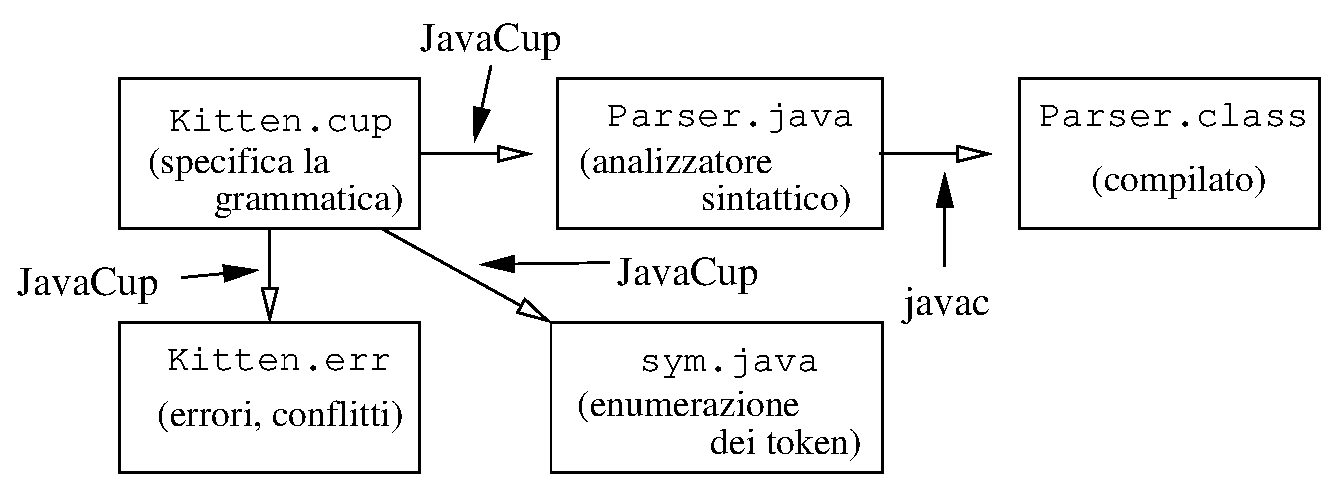
\epsfig{file = java_cup.eps, width = 11cm}
\end{center}
\caption{La generazione dell'analizzatore sintattico tramite JavaCup.}
  \label{fig:java_cup}
\end{figure}
%
\subsection{La specifica dei terminali e dei non terminali}
  \label{subsec:terminals}
%
Il file \texttt{resources/Kitten.cup}
inizia con l'enumerazione dei terminali della grammatica:
%
\begin{verbatim}
  terminal ID, STRING, INTEGER, FLOATING,
           CLASS, EXTENDS, FIELD, METHOD, CONSTRUCTOR, NEW,
           INT, FLOAT, BOOLEAN, VOID,
           COMMA, SEMICOLON, AS, LPAREN, RPAREN,
           LBRACK, RBRACK, LBRACE, RBRACE, DOT, PLUS, MINUS,
           TIMES, DIVIDE, EQ, NEQ, LT, LE, GT, GE, AND, OR, NOT,
           ASSIGN, ARRAY, IF, THEN, ELSE, WHILE, FOR,
           OF, RETURN, NIL, TRUE, FALSE, UMINUS;
\end{verbatim}
%
Si noti che essi, tranne \texttt{UMINUS} (Sezione~\ref{subsec:priorities}),
sono esattamente gli stesso terminali (token) generati
dall'analizzatore lessicale del Capitolo~\ref{chap:lexical}. L'ordine
con cui essi sono enumerati non ha normalmente importanza, ma
ritorneremo su questo aspetto.
Segue quindi una enumerazione dei non terminali\footnote{
Non scriviamo i non terminali
in italico poich\'e si tratta di un file testo che viene passato a JavaCup.}
della grammatica:
%
\begin{verbatim}
  non terminal class;
  non terminal class_members;
  non terminal formals;
  non terminal formals_aux;
  non terminal statements;
  non terminal command;
  non terminal exp;
  non terminal expseq;
  non terminal expseq_aux;
  non terminal lvalue;
  non terminal type;
  non terminal typeplus;
\end{verbatim}
%
Un ben preciso non terminale \`e marcato come non terminale iniziale della
grammatica:
%
\begin{verbatim}
  start with class;
\end{verbatim}
%
Questo significa che un programma Kitten deve essere derivabile a partire
dal non terminale \texttt{class} ovvero, per come daremo le produzioni di
\texttt{class}, che un programma Kitten non \`e altro che una definizione
di una classe, che eventualmente usa altre classi definite in altri file
sorgenti.

Seguono a questo punto le produzioni della grammatica per ogni non terminale
del linguaggio enumerato sopra. Li commenteremo secondo un ordine bottom-up,
partendo \cioe da tipi, espressioni e comandi e andando verso
il non terminale per la classe.
%
\subsection{La specifica dei tipi Kitten}\label{subsec:types_specification}
%
I tipi Kitten sono descritti dalle seguenti produzioni:
%
\begin{verbatim}
  type ::=
     ID
   | BOOLEAN
   | INT
   | FLOAT
   | ARRAY OF type ;
\end{verbatim}
%
La barra verticale indica un'alternativa nella definizione di \texttt{type}.
Si noti che, oltre ai tre tipi primitivi \texttt{boolean}, \texttt{int}
e \texttt{float}, sono previsti dei tipi classe, espressi come il token
\texttt{ID}, nonch\'e il tipo array, definito ricorsivamente.
Il non terminale \texttt{type} \`e usato quando si vuole specificare
il tipo di una variabile, per esempio in una dichiarazione, o in una
espressione, come in un cast. Se vogliamo invece specificare il tipo
di ritorno di un metodo useremo il
non terminale \texttt{typeplus} che ammette anche il tipo \texttt{void}:
%
\begin{verbatim}
  typeplus ::=
     type
   | VOID ;
\end{verbatim}
%
\subsection{La specifica delle espressioni Kitten}
  \label{subsec:expressions_specification}
%
Un'espressione (Sezione~\ref{sec:expressions})
\`e definita in maniera ricorsiva tramite le seguenti produzioni:
%
\begin{verbatim}
  exp ::=
     lvalue                          // leftvalue
   | TRUE                            // la costante true
   | FALSE                           // la costante false
   | INTEGER                         // una costante intera
   | FLOATING                        // una costante in virgola mobile
   | STRING                          // una costante stringa fra apici
   | NIL                             // il riferimento costante nil
   | NEW ID LPAREN expseq RPAREN     // la creazione di un oggetto
   | NEW type LBRACK exp RBRACK      // la creazione di un array
   | exp AS type                     // un cast o conversione di tipo
   | exp PLUS exp                    // un'addizione
   | exp MINUS exp                   // una sottrazione
   | exp TIMES exp                   // una moltiplicazione
   | exp DIVIDE exp                  // una divisione
   | MINUS exp                       // l'opposto di un valore intero
   | exp LT exp                      // <
   | exp LE exp                      // <=
   | exp GT exp                      // >
   | exp GE exp                      // >=
   | exp EQ exp                      // uguaglianza
   | exp NEQ exp                     // disuguaglianza
   | exp AND exp                     // and logico
   | exp OR exp                      // or logico
   | NOT exp                         // negazione logica
   | exp DOT ID LPAREN expseq RPAREN // chiamata di metodo non void
   | LPAREN exp RPAREN ;             // parentesi
\end{verbatim}
%
Tali produzioni dicono in primo luogo che i \emph{leftvalue} sono
espressioni. In effetti, tutte le espressioni possono essere usate
alla destra di un assegnamento (come \emph{rightvalue}) ma
una categoria ristretta di espressioni, dette \emph{leftvalue}, pu\`o
essere usata \emph{anche} alla sinistra di un assegnamento.
A tal fine, tali espressioni devono fare riferimento a una ben precisa
cella di memoria dentro la quale l'assegnamento pu\`o scrivere.
Ci sono solo tre tipi di leftvalue in Kitten:
%
\begin{enumerate}
\item le variabili, come in \texttt{a := 35}; in questo caso l'assegnamento
      modifica la cella di memoria che contiene il valore della variabile
      \texttt{a};
\item i campi degli oggetti, come in \texttt{o.f := a}; in questo caso
      l'assegnamento modifica la cella di memoria che contiene il valore
      del campo \texttt{f} dell'oggetto contenuto nella variabile
      \texttt{o};
\item gli elementi degli array, come in \texttt{arr[i] := a}; in questo caso
      l'assegnamento modifica la cella $i$-esima dell'array \texttt{arr}.
\end{enumerate}
%
Conseguentemente, la specifica dei leftvalue \`e data tramite le seguenti
produzioni:
%
\begin{verbatim}
  lvalue ::=
     ID                              // una variabile
   | exp DOT ID                      // il campo di un oggetto
   | exp LBRACK exp RBRACK ;         // un elemento di un array
\end{verbatim}
%
Si noti che la sintassi di espressioni e leftvalue \`e mutuamente ricorsiva.

Le precedenti produzioni per \texttt{exp} dicono anche
che tutte le costanti del linguaggio sono espressioni:
\cioe \texttt{true}, \texttt{false}, le costanti intere, le costanti in virgola
mobile, le stringhe fra doppi apici e il riferimento \texttt{nil}.
\`E un'espressione anche la creazione di un oggetto come in
\texttt{new Rettangolo(10, 20)}. Questo \e ottenuto tramite la
produzione per \texttt{exp}:
%
\begin{verbatim}
  exp ::= NEW ID LPAREN expseq RPAREN
\end{verbatim}
%
dove \texttt{ID} \`e l'identificatore della classe che si sta istanziando
ed \texttt{expseq} \`e una sequenza, possibilmente vuota, di espressioni
separate da virgole:
%
\begin{verbatim}
  expseq ::=
   | expseq_aux ;

  expseq_aux ::=
     exp
   | exp COMMA expseq_aux ;
\end{verbatim}
%
Si noti che la prima produzione per \texttt{expseq}
\`e una $\varepsilon$-produzione.

La creazione di un array specifica sia il tipo dei suoi elementi che la
dimensione dell'array, come in \texttt{new int[50]}, ed \`e ottenuta tramite
la produzione
%
\begin{verbatim}
  exp ::= NEW type LBRACK exp RBRACK
\end{verbatim}
%
Kitten non ammette la creazione diretta di array multidimensionali. Essi devono
quindi essere creati a partire da un array monodimensionale i cui elementi
sono a loro volta degli array che vanno essi stessi
creati esplicitamente come array monodimensionali.

Il cast viene effettuato in Kitten con la notazione \texttt{as}, come in
\texttt{persona as Studente}. Questa sintassi \`e resa possibile dalla
produzione:
%
\begin{verbatim}
  exp ::= exp AS type
\end{verbatim}
%
Si noti che \texttt{type} non \`e vincolato in alcun modo (tranne a non essere
\texttt{void}, infatti abbiamo usato \texttt{type} e non \texttt{typeplus}).
\`E quindi del tutto lecito scrivere \texttt{12 as float} oppure
\texttt{arr as array of int}. In particolare, la stessa notazione viene
usata sia per le conversioni di tipo (\texttt{12 as float}) che per
i cast veri e propri (\texttt{persona as Studente} oppure
\texttt{arr as array of int}).

Le precedenti produzioni per le espressioni includono le operazioni
binarie, sia aritmetiche (addizione, sottrazione, moltiplicazione e
divisione) che di confronto (maggiore, maggiore o uguale, minore, minore
o uguale, uguale, diverso) che logiche (and logico e or logico).
Infine includono le due operazioni unarie di negazione di interi
(\texttt{MINUS}) e di valori logici (\texttt{NOT}) e l'espressione
per la chiamata di metodo che non ritorna \texttt{void}
(Sezione~\ref{sec:expressions}), ottenuta con la produzione:
%
\begin{verbatim}
  exp ::= exp DOT ID LPAREN expseq RPAREN
\end{verbatim}
%
in cui, come si pu\`o vedere, \`e richiesta la presenza esplicita
del ricevitore della chiamata.

Infine, una espressione fra parentesi tonde viene ancora considerata
come un'espressione. Questo permette per esempio
di cambiare la precedenza degli operatori aritmetici rispetto a quella
di default, descritta nella prossima sezione.
%
\subsection{La specifica della precedenza degli operatori aritmetici}
  \label{subsec:priorities}
%
La grammatica per le espressioni aritmetiche della sezione precedente
\`e chiaramente ambigua. Per esempio, l'espressione
\texttt{2 + a * 4} pu\`o essere interpretata sia come
\texttt{(2 + a) * 4} che come \texttt{2 + (a * 4)}. Abbiamo gi\`a anticipato
che le grammatiche ambigue ci porranno problemi in fase di creazione
dell'analizzatore sintattico, il quale essenzialmente non sa quale delle
due interpretazioni preferire. Sappiamo dall'esperienza con altri linguaggi
di programmazione che la moltiplicazione ha \emph{precedenza} rispetto
all'addizione, per cui l'interpretazione da preferire \`e
\texttt{2 + (a * 4)}. Un problema simile sorge di fronte a espressioni come
\texttt{2 - a - 4} che sono normalmente intese come
\texttt{(2 - a) - 4} piuttosto che come \texttt{2 - (a - 4)}. Si noti che
queste due interpretazioni sono diverse poich\'e, se \texttt{a} valesse
$0$, la prima interpretazione darebbe a
\texttt{2 - a - 4} il valore $-2$ mentre la seconda le darebbe il valore $6$.
In questo caso si tratta di un problema di \emph{associativit\`a}
degli operatori e il fatto che l'interpretazione da preferire sia
\texttt{(2 - a) - 4} significa che gli operatori aritmetici normalmente
\emph{associano a sinistra}.
Queste regole vanno in qualche modo specificate nella grammatica.

Un primo approccio \`e quello di individuare una grammatica non
ambigua che d\`a priorit\`a alla moltiplicazione (e divisione) rispetto
all'addizione (e sottrazione) e che specifica l'associativit\`a a sinistra
degli operatori. Per esempio si potrebbero usare le seguenti produzioni
al posto di quelle della Sezione~\ref{subsec:expressions_specification}:
%
\begin{verbatim}
  exp ::=
     term
   | exp PLUS term
   | exp MINUS term ;
\end{verbatim}
%
\begin{figure}[t]
\[
  \xymatrix{
    & \mathtt{exp}\ar[ld]\ar[d]\ar[rd] \\
  \mathtt{exp}\ar[d] & \mathtt{PLUS} & \mathtt{term}\ar[ld]\ar[d]\ar[rd]\\
  \mathtt{term}\ar[d] & \mathtt{term}\ar[d] &
    \mathtt{TIMES} & \mathtt{factor}\ar[d] \\
  \mathtt{factor}\ar[d] & \mathtt{factor}\ar[d] & & \mathtt{4}\\
  \mathtt{2} & \mathtt{a}\\
  }
\]
\caption{Un albero di derivazione per \texttt{2 + a * 4} tramite una grammatica non ambigua per le espressioni aritmetiche.}
  \label{fig:no_ambiguity}
\end{figure}
%
la quale definisce una \texttt{exp} come una lista non vuota di \texttt{term},
separati da \texttt{+} o \texttt{-}, con associativit\`a a sinistra.
Il nuovo non terminale \texttt{term} viene definito a sua volta come una
lista non vuota di \texttt{factor}, separati da \texttt{*} e \texttt{/},
con associativit\`a a sinistra:
%
\begin{verbatim}
  term ::=
     factor
   | term TIMES factor
   | term DIVIDE factor ;
\end{verbatim}
%
dove
%
\begin{verbatim}
  factor ::= ... altre produzioni per le espressioni ...
\end{verbatim}
%
Con queste produzioni, l'unico albero di derivazione possibile
per \texttt{2 + a * 4} a partire da \texttt{exp} \`e quello mostrato
in Figura~\ref{fig:no_ambiguity}, dove le foglie etichettate come
\texttt{2}, \texttt{a} e \texttt{4} vanno intese come \texttt{INTEGER},
\texttt{ID} e \texttt{INTEGER}, rispettivamente, ma abbiamo preferito
indicare il loro valore lessicale per maggiore chiarezza.

L'uso di una grammatica non ambigua, sebbene possibile, risulta per\`o
scomodo perch\'e, come si vede, occorre strutturare la grammatica in una
maniera non molto intuitiva. Non sar\`a quindi questa la strada seguita
in Kitten. Risulta pi\`u semplice infatti lasciare ambigua la grammatica
ma specificare come risolvere l'ambiguit\`a tramite delle regole
di priorit\`a e associativit\`a per gli operatori binari.
In particolare, basta aggiungere le seguenti dichiarazioni all'interno del
file \texttt{resources/Kitten.cup}:
%
\begin{verbatim}
  precedence left AND, OR;
  precedence left NOT;
  precedence nonassoc EQ, NEQ, LT, LE, GT, GE;
  precedence left PLUS, MINUS;
  precedence left TIMES, DIVIDE;
  precedence left UMINUS;
  precedence left DOT, LBRACK;
\end{verbatim}
%
Queste dichiarazioni enumerano gli operatori di Kitten in ordine di
priorit\`a crescente. Esse indicano inoltre la loro associativit\`a,
la qual cosa ha senso comunque solo per gli operatori binari.
L'effetto di queste dichiarazioni \`e in primo luogo quello di dare priorit\`a
minima agli operatori logici binari e priorit\`a subito maggiore alla
negazione logica. Per esempio, questo fa s\`{\i} che
\texttt{!a \& b} venga interpretato come \texttt{(!a) \& b}.
L'associativit\`a \`e richiesta sinistra, \cosi che per esempio
\texttt{a \& b | c} viene interpretato come \texttt{(a \& b) | c}.
Gli operatori di confronto hanno priorit\`a superiore a quelli
logici, in modo tale che \texttt{a \& b = c} venga interpretato come
\texttt{a \& (b = c)}. Inoltre \`e richiesto che essi non siano
associativi. Questo significa che viene considerato come un errore
scrivere \texttt{a = b = c}. La priorit\`a successiva \`e quella
degli operatori aritmetici, con addizioni e sottrazioni che hanno
priorit\`a inferiore a moltiplicazioni e divisioni. Ancora maggiore
\`e la priorit\`a del token \texttt{UMINUS}. Si noti che tale token non
viene mai ritornato dall'analizzatore lessicale del
Capitolo~\ref{chap:lexical}. Esso \`e un token
fittizio usato solo per avere una priorit\`a maggiore della moltiplicazione
e della divisione. Tale priorit\`a viene data esplicitamente alla produzione
%
\begin{verbatim}
  exp ::= MINUS exp %prec UMINUS
\end{verbatim}
%
per le espressioni. Questo fa s\`{\i} per esempio che l'espressione
\texttt{-a * b} venga interpretato come \texttt{(-a) * b}.
%\cioe dando priorit\`a alla riduzione secondo la precedente
%produzione piuttosto che allo spostamento del token della moltiplicazione.
%
L'ultima precedenza d\`a al punto e alla parentesi quadra
aperta una priorit\`a maggiore
di quella di tutti gli altri operatori. Per esempio, questo permette
di interpretare l'espressione
\texttt{a < b.f} come \texttt{a < (b.f)} piuttosto che
come \texttt{(a < b).f} ed \texttt{a < b[5]} come \texttt{a < (b[5])}
piuttosto che come \texttt{(a < b)[5]}.

Nella Sezione~\ref{subsec:ambiguity} vedremo come queste regole di priorit\`a e
associativit\`a vengono utilizzate da JavaCup per risolvere l'ambiguit\`a
della grammatica.
%
\subsection{La specifica dei comandi Kitten}
  \label{subsec:commands_specification}
%
La specifica dei comandi \`e ricorsiva e utilizza
quella delle espressioni (Sezione~\ref{sec:commands}).
La parte di grammatica che specifica l'insieme dei comandi \`e
formata dalle produzioni:
%
\begin{verbatim}
  command ::=
     lvalue ASSIGN exp  // un assegnamento
   | type ID ASSIGN exp // una dichiarazione di variabile
   | RETURN             // un return da un metodo che ritorna void
   | RETURN exp         // un return da un metodo che non ritorna void
   | IF LPAREN exp RPAREN THEN command  // un if/then
   | IF LPAREN exp RPAREN THEN command
       ELSE command                     // un if/then/else
   | WHILE LPAREN exp RPAREN command    // un ciclo while
   | FOR LPAREN command SEMICOLON exp
       SEMICOLON command RPAREN command // un ciclo for
   | LBRACE statements RBRACE           // uno scope locale
   | LBRACE RBRACE                      // un comando vuoto
   | exp DOT ID LPAREN expseq RPAREN ;  // una chiamata di metodo
\end{verbatim}
%
Osserviamo che queste produzioni lasciano facoltativi
l'\texttt{else} di un \texttt{if} e l'espressione di ritorno di
un comando \texttt{return}. Inoltre esse non impongono
in alcun modo che dentro un metodo che ritorna \texttt{void}
si trovino solo \texttt{return} \emph{senza} espressione di ritorno,
\nec che dentro un metodo che non ritorna \texttt{void} si trovino
\texttt{return} \emph{con} un'espressione di ritorno. Questi vincoli
complicherebbero notevolmente la grammatica. Inoltre non riusciremmo
comunque a controllare che i tipi ritornati corrispondano a quelli
dichiarati per i metodi. Preferiamo invece lasciare questi
(e altri) controlli alla successiva fase di analisi semantica
(Capitolo~\ref{chap:semantical}).

La produzione
%
\begin{verbatim}
  exp ::= LBRACE statements RBRACE
\end{verbatim}
%
definisce uno \emph{scope locale}, \cioe una sequenza non vuota di comandi,
separati da punti e virgola, le cui dichiarazioni restano locali
a tale sequenza stessa (ovvero non sono \piu visibili dopo la
parentesi graffa di chiusura). Il non terminale \texttt{statements}
definisce proprio tale sequenza di comandi:
%
\begin{verbatim}
  statements ::=
     command
   | command SEMICOLON statements ;
\end{verbatim}
%
\subsection{La specifica di una classe Kitten}
  \label{subsec:classes_specification}
%
Definiti comandi ed espressioni, possiamo finalmente definire la sintassi
di una classe, \cioe del non terminale di partenza della grammatica
Kitten (Sezione~\ref{subsec:terminals}). La definizione \`e la seguente:
%
\begin{verbatim}
  class ::=
     CLASS ID LBRACE class_members RBRACE
   | CLASS ID EXTENDS ID LBRACE class_members RBRACE ;
\end{verbatim}
%
Come si pu\`o vedere, l'indicazione della superclasse \`e facoltativa.
Quando manca, si assume implicitamente
che essa sia \texttt{Object}. I membri della
classe sono una lista possibilmente vuota di
dichiarazioni di campi, costruttori e metodi:
%
\begin{verbatim}
  class_members ::=
   | FIELD type ID class_members               // un campo
   | CONSTRUCTOR LPAREN formals RPAREN command
       class_members                           // un costruttore
   | METHOD typeplus ID LPAREN formals RPAREN command
       class_members ;                         // un metodo
\end{verbatim}
%
La prima produzione per \texttt{class\_members}
\`e una $\varepsilon$-produzione, in modo che
una lista di membri di una classe possa anche essere vuota.
Osserviamo che il corpo dei metodi e dei costruttori \`e un comando,
senza obbligo di presenza delle parentesi graffe intorno
al corpo. Inoltre il tipo di ritorno di un metodo \`e un
\texttt{typeplus}, in modo da ammettere anche \texttt{void}
(Sezione~\ref{subsec:types_specification}).
I parametri formali di costruttori e metodi non sono altro che una lista
possibilmente vuota di coppie tipo/nome del parametro, separate da virgola:
%
\begin{verbatim}
  formals ::=
   | formals_aux ;

  formals_aux ::=
     type ID
   | type ID COMMA formals_aux ;
\end{verbatim}
%
Si noti che la prima produzione per \texttt{formals} \`e una
$\varepsilon$-produzione.
%
\subsection{L'interfaccia con l'analizzatore lessicale}
  \label{subsec:jlex_and_java_cup}
%
Specificata la grammatica, occorre ancora indicare, in
\texttt{resources/Kitten.cup}, come interfacciarsi con
l'analizzatore lessicale che abbiamo ottenuto nel Capitolo~\ref{chap:lexical}.
A tal fine, inseriamo fra i delimitatori
\verb!parser code {:! e \verb!:};! del codice che verr\`a
riportato testualmente all'inizio dell'analizzatore sintattico
generato da JavaCup. Tale codice si preoccupa di definire un campo
dell'analizzatore sintattico
di tipo \texttt{lexical.Lexer} e di inizializzarlo all'interno del suo
costruttore con un nuovo analizzatore lessicale. Inoltre, esso fa s\`{\i} che
si possano segnalare degli errori di sintassi tramite la struttura di errore
associata all'analizzatore lessicale appena creato:
%
\begin{verbatim}
  parser code {:
    private Lexer lexer;

    public Parser(Lexer lexer) {
      this.lexer = lexer;
    }

    public ErrorMsg getErrorMsg() {
      return lexer.getErrorMsg();
    }

    public void syntax_error(java_cup.runtime.Symbol token) {
      getErrorMsg().error(token.left, "syntax error");
    }
  :};
\end{verbatim}
%
Il metodo \texttt{syntax\_error()} viene chiamato
dall'analizzatore sintattico quando non riesce a effettuare il parsing
di un programma. Il metodo \texttt{getErrorMsg()} lo usiamo invece per
ottenere la struttura di errore con cui comunicare messaggi di errore
relativi al file sorgente che stiamo processando con un dato analizzatore
sintattico. Tale struttura dati \`e la stessa che abbiamo usato per fare
l'analisi lessicale dello stesso file sorgente. Tale metodo ci sar\`a
utile in futuro quando vorremo segnalare degli errori in fasi successive
di compilazione.

L'ultimo passo \`e di definire in che modo l'analizzatore sintattico
ottiene i token del programma sorgente. Specifichiamo di
utilizzare il metodo \texttt{nextToken()} dell'analizzatore lessicale
(Sezione~\ref{sec:jlex}):
%
\begin{verbatim}
  scan with {:
    return lexer.nextToken();
  :};
\end{verbatim}
%
Si noti che avremmo potuto utilizzare un qualsiasi altro nome al posto di
\texttt{nextToken()}, purch\'e sia lo stesso utilizzato
dall'analizzatore lessicale.

Il risultato della trasformazione di \texttt{resources/Kitten.cup} in un
parser \`e una classe Java \texttt{syntactical/Parser.java} che
contiene un metodo \texttt{parse()}. Chiamando tale metodo si effettua
il parsing del file sorgente, segnalando eventuali errori di sintassi.

Ricordiamo infine che, come mostrato in Figura~\ref{fig:java_cup}, il
programma JavaCup genera anche il file \texttt{syntactical/sym.java} che
contiene una enumerazione dei terminali della grammatica. Tale enumerazione
viene usata anche dall'analizzatore lessicale (Sezione~\ref{sec:jlex}).
%
\javatip{Il fatto che il file \texttt{syntactical/sym.java} venga generato
da JavaCup insieme all'analizzatore sintattico che ne fa uso e che
a sua volta contiene quello
lessicale, il quale usa anch'esso \texttt{syntactical/sym.java}, pone un
fastidioso problema di ciclicit\`a nei casi in cui si vuole modificare
l'insieme dei token del linguaggio Kitten. Occorre allora aggiungere il
token fra le espressioni regolari di \texttt{lexical/Lexer.java} nonch\'e,
manualmente,
nell'enumerazione in \texttt{syntactical/sym.java}, dandogli un codice
arbitrario ma non usato dagli altri token. A questo punto l'analizzatore
lessicale e quello sintattico possono essere compilati. La compilazione
di quest'ultimo genera per\`o un \emph{nuovo} file
\texttt{syntactical/sym.java}, che enumera i token in modo
possibilmente diverso dall'enumerazione manuale che avevamo appena dato.
Occorre ricompilare l'analizzatore lessicale per far s\`{\i} che i due
analizzatori siano finalmente sincronizzati sulla stessa enumerazione.}
%
\section{Il parsing $\mathit{LL}$}\label{sec:ll}
%
Descriviamo in questa sezione il modo pi\`u semplice, ma purtroppo anche
meno potente, per costruire un analizzatore sintattico a partire
da una grammatica. Si consideri la grammatica in Figura~\ref{fig:ll1_grammar}.
%
\begin{figure}[t]
\begin{align*}
  \mathit{I}&\to\mathit{com}\ \mathtt{\$}\\
  \mathit{com}&\to\mathit{exp}\ \mathtt{ASSIGN}\ \mathtt{INTEGER}\\
  \mathit{exp}&\to\mathtt{ID}\\
  \mathit{exp}&\to\mathtt{INTEGER}\\
  \mathit{exp}&\to\mathtt{MINUS}\ \mathit{exp}
\end{align*}
\caption{Una grammatica $\mathit{LL}(1)$.}\label{fig:ll1_grammar}
\end{figure}
%
La prima produzione indica che un file sorgente che rispetta le regole
di questa grammatica deve contenere un $\mathit{com}$ seguito da
un carattere \texttt{\$}, che tradizionalmente
indica la fine del file sorgente (il token di end of file).
Quando una grammatica contiene solo una produzione per il non terminale
iniziale $I$, la quale inoltre termina con il token \texttt{\$},
si dice che essa \`e
\emph{aumentata}\footnote{L'aumento di una grammatica \`e ottenuto
automaticamente in JavaCup tramite la direttiva \texttt{start with}. In questo esempio
con \texttt{start with com}.}.
Il senso \`e che questa produzione impone che non ci siano
caratteri in pi\`u dopo il $\mathit{com}$.

Supponiamo quindi di essere posizionati all'inizio del file sorgente.
Affinch\'e il sorgente sia corretto, davanti a noi deve esserci un
$\mathit{com}$ e poi la fine del file. Supponiamo di essere
posizionati da qualche parte all'interno del file sorgente e di dovere
riconoscere un $\mathit{com}$. Per come \`e scritta la grammatica,
l'unica speranza \`e che dinanzi a noi ci sia un $\mathit{exp}$ seguito dal
token $\mathtt{ASSIGN}$ seguito dal token $\mathtt{INTEGER}$.
Supponiamo infine di essere posizionati da qualche parte nel file sorgente
e di dovere riconoscere un $\mathit{exp}$. Questa volta abbiamo tre
possibilit\`a, mutuamente esclusive:
%
\begin{enumerate}
\item davanti a noi c'\`e il token $\mathtt{ID}$
\item oppure davanti a noi c'\`e il token $\mathtt{INTEGER}$
\item oppure davanti a noi c'\`e il token $\mathtt{MINUS}$ e siamo
      poi capaci di riconoscere, ricorsivamente, un altro $\mathit{exp}$.
\end{enumerate}

Questo semplice ragionamento ci permette di scrivere dei metodi privati
dell'analizzatore sintattico, \emph{uno per ogni non terminale},
i quali si occupano di riconoscere il corrispondente
non terminale della grammatica.
La Figura~\ref{fig:java_ll1} mostra l'implementazione in Java di tali metodi.
Si noti che si tratta di un raffinamento del codice che abbiamo visto nella
Sezione~\ref{subsec:jlex_and_java_cup}.
%
\begin{figure}[t]
{\small
\begin{verbatim}
import syntactical.sym;

public class Parser {
  private Lexer lexer;
  private java_cup.runtime.Symbol lookahead;

  public Parser(Lexer lexer) {
    this.lexer = lexer; lookahead = lexer.nextToken();
  }
  ... syntax_error ...
  private void eat(java_cup.runtime.Symbol token) {
    if (lookahead.sym != token.sym) syntax_error(lookahead);
    lookahead = lexer.nextToken();     
  }
  public void parse() { parseI(); }
  private void parseI() { parseCom(); eat(sym.EOF); }
  private void parseCom() { parseExp(); eat(sym.ASSIGN); eat(sym.INTEGER); }
  private void parseExp() {
    switch (lookahead.sym) {
      case sym.ID: eat(sym.ID); break;
      case sym.INTEGER: eat(sym.INTEGER); break;
      case sym.MINUS: eat(sym.MINUS); parseExp();
      default: syntax_error(lookahead);
    }
  }
}
\end{verbatim}
}
\caption{L'implementazione in Java di un parser $\mathit{LL}(1)$
         per la grammatica in
         Figura~\ref{fig:ll1_grammar}.}\label{fig:java_ll1}
\end{figure}
%
Il metodo ausiliario
\texttt{eat()} impone che davanti a noi ci sia il token indicato
come parametro. In caso contrario segnala un errore di sintassi.
L'implementazione di \texttt{parseI()}, \texttt{parseCom()}
e \texttt{parseExp()} ricalca il ragionamento fatto sopra. Si noti
in particolare che \texttt{parseExp()} \`e ricorsivo e che il suo
comportamento \`e guidato dal token, detto \emph{lookahead},
che ci troviamo davanti al momento
della sua chiamata. Se tale token non \`e nessuno dei tre leciti, segnaliamo
un errore di sintassi. Affinch\'e il file sorgente sia
corretto, occorre poter riconoscere il non terminale $I$ all'inizio di tale
file. Questo \`e proprio quello che facciamo nel metodo \texttt{parse()}
che effettua il parsing del file sorgente.

La generazione del codice in Figura~\ref{fig:java_ll1} pu\`o essere
fatta in maniera automatica a partire dalla grammatica in
Figura~\ref{fig:ll1_grammar} poich\'e i metodi del tipo
\texttt{parse}$N$ ricalcano direttamente l'insieme delle produzioni
per il non terminale $N$. L'unica richiesta \`e che sia possibile,
per ogni non terminale definito da pi\`u di una produzione, decidere
quale produzione utilizzare sulla base del token che si ha di fronte.
Per esempio, il non terminale $\mathit{exp}$ \`e definito da tre
produzioni in Figura~\ref{fig:ll1_grammar} ed \`e sempre possibile
decidere quale delle tre utilizzare guardando il token che ci sta
davanti, come mostrato nell'implementazione in Figura~\ref{fig:java_ll1}.
Il motivo \`e che le tre produzioni hanno lati destri che \emph{iniziano} con
token distinti, per cui non c'\`e alcun token che d\`a origine ad
ambiguit\`a su quale delle tre produzioni applicare.
Questo ragionamento ci dice che per costruire un programma come quello
in Figura~\ref{fig:java_ll1} occorre conoscere, per ogni non terminale
definito dalle produzioni
$L\to r_1,\ldots,L\to r_n$ con $n\ge 2$, qual \`e l'insieme dei token con cui
pu\`o cominciare ciascuno dei lati destri $r_1,\ldots,r_n$ e che inoltre
occorre che tali insiemi siano disgiunti. Per esempio,
il lato destro della produzione $\mathtt{MINUS}\ \mathit{exp}$ in
Figura~\ref{fig:ll1_grammar} inizia con l'insieme di token
$\{\mathtt{MINUS}\}$.

Calcolare questi inizi non \`e \cosi semplice
come pu\`o sembrare a prima vista, dal momento che i lati destri delle
produzioni potrebbero cominciare con un non terminale, come
in $\mathit{exp}\to\mathit{exp}\ \mathtt{PLUS}\ \mathit{exp}$,
o potrebbero essere \emph{annullabili}, come in $\mathit{exp}\to\varepsilon$,
nel qual caso non c'\`e alcun token con cui essi iniziano e occorre
invece guardare quali token potrebbero \emph{seguire} il lato sinistro
della produzione, in questo caso $\mathit{exp}$, per capire quando
selezionare la produzione.
Affrontiamo questi problemi formalmente nella sezione seguente.
%
\subsection{Gli insiemi $\nullable$, $\first$ e $\follow$.}
  \label{subsec:sets}
%
Abbiamo accennato al fatto che una $\varepsilon$-produzione del tipo
$\mathit{exp}\to\varepsilon$ deve essere
trattata con cura nella costruzione del parsing. Pi\`u in generale, la stessa
attenzione deve essere usata per tutte quelle produzioni il cui lato
destro \`e \emph{annullabile}, cio\`e \`e una forma sentenziale
da cui \`e possibile derivare $\varepsilon$.
%
\begin{definition}\label{def:nullable}
Data una grammatica $G$ e una forma sentenziale $\alpha$, diciamo che
$\alpha$ \`e \emph{annullabile in $G$} se e solo se
$\alpha\Rightarrow^*_G\varepsilon$.
L'insieme dei non terminali annullabili di $G$ \`e indicato come
$\nullable_G$ (di solito omettiamo $G$ se essa \`e chiara dal contesto).
\end{definition}
%
\noindent
Si noti che basta conoscere i non terminali annullabili per poter calcolare,
in maniera composizionale,
l'annullabilit\`a di una qualsiasi altra forma sentenziale.
%
\begin{proposition}\label{prop:extend_nullable}
Sia $\langle T,N,I,P\rangle$ una grammatica e $\nu\subseteq N$.
Sia $\alpha$ una forma sentenziale e definiamo $\nullable(\alpha,\nu)$ come
segue:
\begin{equation}\label{eq:nullable}
\begin{split}
  \nullable(\varepsilon,\nu)&=\mathit{true}\\
  \nullable(t,\nu)&=\mathit{false}\quad\text{per ogni $t\in T$}\\
  \nullable(n,\nu)&=(n\in\nu)\quad\text{per ogni $n\in N$}\\
  \nullable(\alpha_1\alpha_2,\nu)&=\nullable(\alpha_1,\nu)\wedge
    \nullable(\alpha_2,\nu).
\end{split}
\end{equation}
Se $\nu$ \`e l'insieme dei non terminali annullabili in $G$, allora
$\alpha$ \`e annullabile se e solo se $\nullable(\alpha,\nu)$. In tal caso
scriviamo $\nullable(\alpha)$ piuttosto che $\nullable(\alpha,\nu)$.
\end{proposition}
%
Il calcolo dell'insieme $\nullable$ per una grammatica si effettua
come un calcolo di punto fisso. Partendo da un insieme vuoto $\phi^0$
di annullabili, si aggiungono prima i nonterminali che hanno una produzione
con $\varepsilon$ come lato destro, ottenendo $\phi^1$. Quindi,
se $\phi^1\not=\phi^0$, si aggiungono i non terminali che hanno alla
destra solo non terminali e tutti annullabili poich\'e in $\phi^1$.
Si ottiene \cosi $\phi^2$. Il procedimento viene iterato finch\'e
non si raggiunge un punto fisso, cio\`e un $\phi^k$ tale che
$\phi^k=\phi^{k+1}$.
%
\begin{proposition}\label{prop:nullable}
Sia $\langle T,N,I,P\rangle$ una grammatica e $\nu\subseteq N$.
Definiamo
\[
  \phi(\nu)=\{L\mid L\to r\in P\text{ e }\nullable(r,\nu)\}.
\]
Si ha $\nullable_G=\lfp(\phi)$, dove $\lfp(\phi)$ \`e il minimo punto
fisso di $\phi$, calcolabile come $\lim_{i\to\infty}\phi^i$, con
\begin{align*}
  \phi^0&=\emptyset\\
  \phi^{i+1}&=\phi(\phi^i)\quad\text{per ogni $i\ge 0$.}
\end{align*}
\end{proposition}
%
Questo risultato pu\`o sembrare complesso ma \`e in realt\`a di facile
applicazione. Essenzialmente dice di cominciare il calcolo
di $\nullable$ dall'insieme vuoto e di aggiungervi man mano quei non terminali
che stanno alla sinistra di una produzione il cui lato destro risulta
annullabile secondo le equazioni~\eqref{eq:nullable}. Questo calcolo deve
essere iterato finch\'e non \`e \piu possibile aggiungere nuovi non terminali.
Si noti che l'uso di $\infty$ nel limite della Proposizione~\ref{prop:nullable}
non significa che serve un numero infinito di iterazioni, poich\'e l'insieme
dei non terminali di una data grammatica
\`e finito e quindi tale limite verr\`a sicuramente raggiunto
in un numero di iterazioni pari, \emph{al massimo}, al numero dei non terminali
della grammatica. Dopo tale numero di iterazioni, il calcolo si sar\`a
stabilizzato.

Vediamo un primo esempio. Vogliamo calcolare i non terminali annullabili
della grammatica in Figura~\ref{fig:ll1_grammar}.
Cominciamo dall'insieme vuoto, che scriviamo con una tabella che dice
che nessun non terminale \`e al momento considerato annullabile:
%
\begin{center}
\begin{tabular}{|r||c|}
\multicolumn{2}{c}{$\nullable$}\\\hline\hline
 & $\phi^0$ \\\hline
$I$ & $\mathit{false}$ \\\hline
$\mathit{com}$ & $\mathit{false}$ \\\hline
$\mathit{exp}$ & $\mathit{false}$\\\hline
\end{tabular}
\end{center}
%
A questo punto dobbiamo considerare tutte le produzioni della grammatica e
marcare come annullabili i non terminali alla sinistra di una produzione
il cui lato destro risulta annullabile secondo le
equazioni~\eqref{eq:nullable}. Dal momento che tutti i lati destri in
Figura~\ref{fig:ll1_grammar} contengono almeno un terminale, nessuno di essi
\`e annullabile e otteniamo
%
\begin{equation}\label{tab:nullable_ll1_grammar}
\mbox{
\begin{tabular}{|r||c|c|}
\multicolumn{3}{c}{$\nullable$}\\\hline\hline
 & $\phi^0$ & $\phi^1$ \\\hline
$I$ & $\mathit{false}$ & $\mathit{false}$ \\\hline
$\mathit{com}$ & $\mathit{false}$ & $\mathit{false}$ \\\hline
$\mathit{exp}$ & $\mathit{false}$ & $\mathit{false}$ \\\hline
\end{tabular}
}
\end{equation}
%
Basta osservare che $\phi^0=\phi^1$ per concludere che abbiamo gi\`a
raggiunto il punto fisso, per cui $\nullable=\phi^1=\emptyset$.

Si consideri adesso la grammatica in Figura~\ref{fig:grammar_lists}.
%
\begin{figure}[t]
\begin{align*}
  I&\to L\mathtt{\$}\\
  L&\to AB\\
  A&\to\varepsilon\\
  A&\to\mathtt{a}A\\
  B&\to\varepsilon\\
  B&\to\mathtt{b}B
\end{align*}
\caption{Un'altra grammatica $\mathit{LL}(1)$.}\label{fig:grammar_lists}
\end{figure}
%
Ancora una volta, partiamo dall'insieme vuoto di non terminali annullabili:
%
\begin{center}
\begin{tabular}{|r||c|}
\multicolumn{2}{c}{$\nullable$}\\\hline\hline
 & $\phi^0$ \\\hline
$I$ & $\mathit{false}$ \\\hline
$L$ & $\mathit{false}$ \\\hline
$A$ & $\mathit{false}$ \\\hline
$B$ & $\mathit{false}$\\\hline
\end{tabular}
\end{center}
%
A questo punto consideriamo le produzioni in Figura~\ref{fig:grammar_lists}.
Il lato destro di $I\to L\mathtt{\$}$ non \`e annullabile in $\phi^0$ poich\'e
contiene il terminale $\mathtt{\$}$:
\[
  \nullable(L\mathtt{\$},\phi^0)=\mathit{false}.
\]
Il lato destro di $L\to AB$ non \`e annullabile in $\phi^0$ poich\'e
nessuno dei due non terminali $A$ e $B$ \`e annullabile in $\phi^0$:
\[
  \nullable(AB,\phi^0)=\mathit{false}.
\]
Il lato destro di $A\to\varepsilon$ \`e annullabile in $\phi^0$:
\[
  \nullable(\varepsilon,\phi^0)=\mathit{true}
\]
\cosi come il lato destro di $B\to\varepsilon$. I lati destri di
$A\to\mathtt{a}A$ e $B\to\mathtt{b}B$ non sono annullabili in $\phi^0$ dal
momento che contengono un terminale:
\[
  \nullable(\mathtt{a}A,\phi^0)=\nullable(\mathtt{b}B,\phi^0)=\mathit{false}.
\]
Concludiamo che $\phi^1$ \`e come indicato in questa tabella:
%
\begin{center}
\begin{tabular}{|r||c|c|}
\multicolumn{3}{c}{$\nullable$}\\\hline\hline
 & $\phi^0$ & $\phi^1$ \\\hline
$I$ & $\mathit{false}$ & $\mathit{false}$ \\\hline
$L$ & $\mathit{false}$ & $\mathit{false}$ \\\hline
$A$ & $\mathit{false}$ & $\mathit{true}$ \\\hline
$B$ & $\mathit{false}$ & $\mathit{true}$ \\\hline
\end{tabular}
\end{center}
%
Dal momento che $\phi^0\not=\phi^1$, non abbiamo ancora raggiunto il punto
fisso e dobbiamo calcolare $\phi^2$. L'unica differenza rispetto al calcolo
di $\phi^1$ \`e che adesso
\[
  \nullable(AB,\phi^1)=\mathit{true}
\]
dal momento che sia $A$ che $B$ sono annullabili in $\phi^1$. Concludiamo che
$\phi^2$ \`e come indicato nella seguente tabella:
%
\begin{center}
\begin{tabular}{|r||c|c|c|}
\multicolumn{4}{c}{$\nullable$}\\\hline\hline
 & $\phi^0$ & $\phi^1$ & $\phi^2$ \\\hline
$I$ & $\mathit{false}$ & $\mathit{false}$ & $\mathit{false}$ \\\hline
$L$ & $\mathit{false}$ & $\mathit{false}$ & $\mathit{true}$ \\\hline
$A$ & $\mathit{false}$ & $\mathit{true}$ & $\mathit{true}$ \\\hline
$B$ & $\mathit{false}$ & $\mathit{true}$ & $\mathit{true}$ \\\hline
\end{tabular}
\end{center}
%
Dal momento che $\phi^1\not=\phi^2$ dobbiamo calcolare $\phi^3$. Il suo calcolo
risulta identico a quello di $\phi^2$ per cui in definitiva otteniamo:
%
\begin{equation}\label{tab:grammar_lists_nullable}
\begin{tabular}{|r||c|c|c|c|}
\multicolumn{5}{c}{$\nullable$}\\\hline\hline
 & $\phi^0$ & $\phi^1$ & $\phi^2$ & $\phi^3$ \\\hline
$I$ & $\mathit{false}$ & $\mathit{false}$ & $\mathit{false}$ & $\mathit{false}$\\\hline
$L$ & $\mathit{false}$ & $\mathit{false}$ & $\mathit{true}$ & $\mathit{true}$\\\hline
$A$ & $\mathit{false}$ & $\mathit{true}$ & $\mathit{true}$ & $\mathit{true}$\\\hline
$B$ & $\mathit{false}$ & $\mathit{true}$ & $\mathit{true}$ & $\mathit{true}$\\\hline
\end{tabular}
\end{equation}
%
ovvero $\phi^2=\phi^3$ \`e il punto fisso cercato e quindi
$\nullable=\{L,A,B\}$.
%
\greycomment{La funzione $\phi$ della Proposizione~\ref{prop:nullable} \`e
monotona crescente. Conseguentemente, l'insieme dei non terminali considerati
annullabili non pu\`o che crescere durante il calcolo del punto fisso.
Questa osservazione, che \`e alla base dell'esistenza stessa del punto
fisso cercato, implica anche che se durante il calcolo di una tabella per
$\nullable$ vediamo decrescere l'insieme degli annullabili allora abbiamo
sicuramente fatto un errore.}

\mbox{}\\

Possiamo adesso definire l'insieme dei terminali con cui cominciano
le forme sentenziali derivabili da un'altra forma sentenziale.
%
\begin{definition}\label{def:first}
Data una grammatica $G$ e una forma sentenziale $\alpha$, diciamo che un
terminale $t$ \`e un \emph{inizio} di $\alpha$ se e solo se
$\alpha\Rightarrow^*_Gt\beta$ per qualche forma sentenziale $\beta$.
L'insieme degli inizi di un non terminale
$N$ \`e indicato come $\first_G(N)$, con $G$
normalmente omessa quando \`e chiara dal contesto.
\end{definition}
%
\noindent
Basta conoscere gli inizi dei non terminali
per dedurre quelli di una qualsiasi forma sentenziale.
%
\begin{proposition}\label{prop:extend_first}
Sia $\langle T,N,I,P\rangle$ una grammatica e
$\nu:N\mapsto\wp(T)$ una funzione che assegna a ciascun non terminale
un insieme di terminali.
Sia $\alpha$ una forma sentenziale e definiamo $\first(\alpha,\nu)$ come
segue:
\begin{equation}\label{eq:first}
\begin{split}
  \first(\varepsilon,\nu)&=\emptyset\\
  \first(t,\nu)&=\{t\}\quad\text{per ogni $t\in T$}\\
  \first(n,\nu)&=\nu(n)\quad\text{per ogni $n\in N$}\\
  \first(\alpha_1\alpha_2,\nu)&=\begin{cases}
    \first(\alpha_1,\nu) & \text{se $\alpha_1$ non \`e annullabile}\\
    \first(\alpha_1,\nu)\cup\first(\alpha_2,\nu) &
      \text{se $\alpha_1$ \`e annullabile.}
  \end{cases}
\end{split}
\end{equation}
Se $\nu$ assegna a ciascun non terminale l'insieme dei suoi inizi,
allora gli inizi di $\alpha$ sono esattamente $\first(\alpha,\nu)$.
In tal caso scriviamo $\first(\alpha)$ piuttosto che $\first(\alpha,\nu)$.
\end{proposition}
%
\noindent
Si noti che la definizione dei $\first$ richiede la conoscenza dei $\nullable$.
In particolare, i $\nullable$ sono usati nel calcolo degli inizi di una
forma sentenziale del tipo $\alpha_1\alpha_2$: i suoi inizi sono infatti
gli inizi di $\alpha_1$ ma, se $\alpha_1$ \`e annullabile, bisogna aggiungere
anche gli inizi di $\alpha_2$.

Anche il calcolo degli insiemi $\first$ per una grammatica si effettua
come un calcolo di punto fisso. Inizialmente gli inizi di ciascun non
terminale sono considerati vuoti ($\phi^0$). Quindi si aggiungono
agli inizi di ciascun non terminale l'insieme dei terminali con cui
inizia il lato destro di una produzione per tale non terminale.
Per calcolare come iniziano i lati destri delle produzioni
si usa l'approssimazione precedente, quindi all'inizio si usa $\phi^0$.
Si ottengono \cosi delle approssimazioni successive $\phi^1$, $\phi^2$, \ldots
finch\'e non si raggiunge il punto fisso, cio\`e un $k$ tale che
$\phi^k=\phi^{k+1}$.
%
\begin{proposition}\label{prop:first}
Sia $\langle T,N,I,P\rangle$ una grammatica e $\nu:N\mapsto\wp(T)$. Definiamo
\[
  \phi(\nu)(L)=\bigcup\limits_{L\to r\in P}\first(r,\nu),
\]
per ogni $L\in N$.
Si ha $\first_G=\lfp(\phi)$, dove $\lfp(\phi)$ \`e il minimo punto
fisso di $\phi$, calcolabile come $\lim_{i\to\infty}\phi^i$, con
\begin{align*}
  \phi^0(L)&=\emptyset\\
  \phi^{i+1}(L)&=\phi(\phi^i)(L)\quad\text{per ogni $i\ge 0$}
\end{align*}
e per ogni $L\in N$.
\end{proposition}

Mostriamo per esempio il calcolo degli inizi dei non terminali
della grammatica in Figura~\ref{fig:ll1_grammar}. Useremo una tabella
che rappresenta le approssimazioni $\phi^i$, indicando per ciascun
non terminale l'insieme degli inizi gi\`a calcolati. All'inizio tali insiemi
sono vuoti:
%
\begin{center}
\begin{tabular}{|r||c|}
\multicolumn{2}{c}{$\first$}\\\hline\hline
 & $\phi^0$ \\\hline
$I$ & $\emptyset$ \\\hline
$\mathit{com}$ & $\emptyset$ \\\hline
$\mathit{exp}$ & $\emptyset$\\\hline
\end{tabular}
\end{center}
%
Per calcolare $\phi^1$ dobbiamo considerare ciascuna produzione della
grammatica. La produzione $I\to\mathit{com}\ \mathtt{\$}$, dal momento
che $\mathit{com}$ non \`e annullabile
(tabella~\eqref{tab:nullable_ll1_grammar}), implica
che $\phi^1(\mathit{I})=\first(\mathit{com}\ \mathtt{\$},\phi^0)
=\phi^0(\mathit{com})=\emptyset$. La produzione
$\mathit{com}\to\mathit{exp}\ \mathtt{ASSIGN}\ \mathtt{INTEGER}$,
dal momento che $\mathit{exp}$ non \`e annullabile,
implica che $\phi^1(\mathit{com})=
\first(\mathit{exp}\ \mathtt{ASSIGN}\ \mathtt{INTEGER},\phi^0)=
\phi^0(\mathit{exp})=\emptyset$. Le tre produzioni
$\mathit{exp}\to\mathtt{ID}$, $\mathit{exp}\to\mathtt{INTEGER}$ ed
$\mathit{exp}\to\mathtt{MINUS}\ \mathit{exp}$ implicano che
$\phi^1(\mathit{exp})=\first(\mathtt{ID},\phi^0)\cup
\first(\mathtt{INTEGER},\phi^0)\cup\first(\mathtt{MINUS}\ \mathit{exp},\phi^0)
=\{\mathtt{ID},\mathtt{INTEGER},\mathtt{MINUS}\}$. In conclusione otteniamo:
%
\begin{center}
\begin{tabular}{|r||c|c|}
\multicolumn{3}{c}{$\first$}\\\hline\hline
 & $\phi^0$ & $\phi^1$ \\\hline
$I$ & $\emptyset$ & $\emptyset$ \\\hline
$\mathit{com}$ & $\emptyset$ & $\emptyset$ \\\hline
$\mathit{exp}$ & $\emptyset$ & $\{\mathtt{ID},\mathtt{INTEGER},
  \mathtt{MINUS}\}$\\\hline
\end{tabular}
\end{center}
%
Dal momento che $\phi^0\not=\phi^1$, non abbiamo ancora ottenuto il punto
fisso e dobbiamo calcolare $\phi^2$. Il procedimento \`e simile a quello
per calcolare $\phi^1$, con l'unica differenza che adesso
$\phi^1(\mathit{com})=
\first(\mathit{exp}\ \mathtt{ASSIGN}\ \mathtt{INTEGER},\phi^1)=
\phi^1(\mathit{exp})=\{\mathtt{ID},\mathtt{INTEGER},\mathtt{MINUS}\}$.
Otteniamo quindi la tabella:
%
\begin{center}
\begin{tabular}{|r||c|c|c|}
\multicolumn{4}{c}{$\first$}\\\hline\hline
 & $\phi^0$ & $\phi^1$ & $\phi^2$ \\\hline
$I$ & $\emptyset$ & $\emptyset$ & $\emptyset$ \\\hline
$\mathit{com}$ & $\emptyset$ & $\emptyset$ & $\{\mathtt{ID},\mathtt{INTEGER},\mathtt{MINUS}\}$\\\hline
$\mathit{exp}$ & $\emptyset$ & $\{\mathtt{ID},\mathtt{INTEGER},
  \mathtt{MINUS}\}$ & $\{\mathtt{ID},\mathtt{INTEGER},\mathtt{MINUS}\}$\\\hline
\end{tabular}
\end{center}
%
Abbiamo ancora $\phi^1\not=\phi^2$ per cui dobbiamo calcolare
$\phi^3$. L'unica differenza \`e che adesso otteniamo
$\phi^3(\mathit{I})=\first(\mathit{com}\ \mathtt{\$},\phi^2)
=\phi^2(\mathit{com})=\{\mathtt{ID},\mathtt{INTEGER},\mathtt{MINUS}\}$.
In conclusione otteniamo la tabella:
%
\begin{equation}\label{tab:first_ll1_grammar}
\mbox{
\begin{tabular}{|r||c|c|c|c|}
\multicolumn{5}{c}{$\first$}\\\hline\hline
 & $\phi^0$ & $\phi^1$ & $\phi^2$ & $\phi^3$ \\\hline
$I$ & $\emptyset$ & $\emptyset$ & $\emptyset$ & $\{\mathtt{ID},\mathtt{INTEGER},\mathtt{MINUS}\}$\\\hline
$\mathit{com}$ & $\emptyset$ & $\emptyset$ & $\{\mathtt{ID},\mathtt{INTEGER},\mathtt{MINUS}\}$ & $\{\mathtt{ID},\mathtt{INTEGER},\mathtt{MINUS}\}$\\\hline
$\mathit{exp}$ & $\emptyset$ & $\{\mathtt{ID},\mathtt{INTEGER},
  \mathtt{MINUS}\}$ & $\{\mathtt{ID},\mathtt{INTEGER},\mathtt{MINUS}\}$ &
  $\{\mathtt{ID},\mathtt{INTEGER},\mathtt{MINUS}\}$\\\hline
\end{tabular}
}
\end{equation}
%
Si pu\`o verificare che se calcolassimo $\phi^4$ otterremmo
$\phi^4=\phi^3$, per cui abbiamo raggiunto il punto fisso e possiamo dire
che gli inizi dei non terminali della grammatica in
Figura~\ref{fig:ll1_grammar} sono sempre $\{\mathtt{ID},\mathtt{INTEGER},
\mathtt{MINUS}\}$.
%
\greycomment{Anche la funzione $\phi$ della Proposizione~\ref{prop:first} \`e
monotona crescente, per cui gli insiemi di inizi calcolati durante le
iterazioni di punto fisso non possono mai decrescere. Se quindi
essi decrescessero \`e perch\'e abbiamo fatto un errore nel calcolo.}

\mbox{}\\

L'esempio precedente \`e relativamente semplice dal momento che
nessun non terminale \`e annullabile nella grammatica in
Figura~\ref{fig:ll1_grammar}. Consideriamo invece la grammatica
in Figura~\ref{fig:grammar_lists}, di cui avevamo determinato che i non
terminali annullabili sono $A$, $B$ ed $L$. Il calcolo degli inizi comincia
con l'insieme vuoto di inizi per ciascun non terminale:
%
\begin{center}
\begin{tabular}{|r||c|}
\multicolumn{2}{c}{$\first$}\\\hline\hline
    & $\phi^0$\\\hline
$I$ & $\emptyset$\\\hline
$L$ & $\emptyset$ \\\hline
$A$ & $\emptyset$ \\\hline
$B$ & $\emptyset$ \\\hline
\end{tabular}
\end{center}
%
Per calcolare $\phi^1$, consideriamo le produzioni della grammatica.
Da $I\to L\mathtt{\$}$ concludiamo che
\[
  \phi^1(I)=\first(L\mathtt{\$},\phi^0)=\first(L,\phi^0)\cup
    \first(\mathtt{\$},\phi^0)=\emptyset\cup\{\mathtt{\$}\}=\{\mathtt{\$}\}.
\]
Si noti che questo \`e una conseguenza del fatto che $L$ \`e annullabile,
come abbiamo ricordato. Otteniamo inoltre
\[
  \phi^1(L)=\first(AB,\phi^0)=\first(A,\phi^0)\cup\first(B,\phi^0)
    =\emptyset\cup\emptyset=\emptyset
\]
poich\'e anche $A$ \`e annullabile. Infine abbiamo
\[
  \phi^1(A)=\first(\varepsilon,\phi^0)\cup\first(\mathtt{a}A,\phi^0)
    =\emptyset\cup\first(\mathtt{a},\phi^0)=\first(\mathtt{a},\phi^0)=
    \{\mathtt{a}\}.
\]
Si noti che questo \`e una conseguenza del fatto che $\mathtt{a}$ non \`e
annullabile. Similmente otteniamo $\phi^1(B)=\{\mathtt{b}\}$. In conclusione:
%
\begin{center}
\begin{tabular}{|r||c|c|}
\multicolumn{3}{c}{$\first$}\\\hline\hline
    & $\phi^0$ & $\phi^1$\\\hline
$I$ & $\emptyset$ & $\{\mathtt{\$}\}$\\\hline
$L$ & $\emptyset$ & $\emptyset$ \\\hline
$A$ & $\emptyset$ & $\{\mathtt{a}\}$ \\\hline
$B$ & $\emptyset$ & $\{\mathtt{b}\}$ \\\hline
\end{tabular}
\end{center}
%
Dal momento che $\phi^1\not=\phi^0$ dobbiamo calcolare $\phi^2$. L'unica
differenza sar\`a nel calcolo di $\phi^2(L)$, dal momento che adesso,
ricordando che $A$ \`e annullabile, otteniamo
\[
  \phi^2(L)=\first(AB,\phi^1)=\first(A,\phi^1)\cup\first(B,\phi^1)=
    \{\mathtt{a}\}\cup\{\mathtt{b}\}=\{\mathtt{a},\mathtt{b}\}.
\]
Otteniamo quindi la tabella
%
\begin{center}
\begin{tabular}{|r||c|c|c|}
\multicolumn{4}{c}{$\first$}\\\hline\hline
    & $\phi^0$ & $\phi^1$ & $\phi^2$\\\hline
$I$ & $\emptyset$ & $\{\mathtt{\$}\}$ & $\{\mathtt{\$}\}$\\\hline
$L$ & $\emptyset$ & $\emptyset$ & $\{\mathtt{a},\mathtt{b}\}$ \\\hline
$A$ & $\emptyset$ & $\{\mathtt{a}\}$ & $\{\mathtt{a}\}$ \\\hline
$B$ & $\emptyset$ & $\{\mathtt{b}\}$ & $\{\mathtt{b}\}$ \\\hline
\end{tabular}
\end{center}
%
Poich\'e $\phi^2\not=\phi^1$ dobbiamo ancora calcolare $\phi^3$. L'unica
differenza \`e che adesso otteniamo
\[
  \phi^3(I)=\first(L\mathtt{\$},\phi^2)=\first(L,\phi^2)\cup
    \first(\mathtt{\$},\phi^2)=\{\mathtt{a},\mathtt{b}\}\cup\{\mathtt{\$}\}
    =\{\mathtt{a},\mathtt{b},\mathtt{\$}\}.
\]
Otteniamo quindi la tabella
%
\begin{equation}\label{tab:grammar_lists_first}
\mbox{
\begin{tabular}{|r||c|c|c|c|}
\multicolumn{5}{c}{$\first$}\\\hline\hline
    & $\phi^0$ & $\phi^1$ & $\phi^2$ & $\phi^3$ \\\hline
$I$ & $\emptyset$ & $\{\mathtt{\$}\}$ & $\{\mathtt{\$}\}$ & $\{\mathtt{a},\mathtt{b},\mathtt{\$}\}$ \\\hline
$L$ & $\emptyset$ & $\emptyset$ & $\{\mathtt{a},\mathtt{b}\}$ & $\{\mathtt{a},\mathtt{b}\}$ \\\hline
$A$ & $\emptyset$ & $\{\mathtt{a}\}$ & $\{\mathtt{a}\}$ & $\{\mathtt{a}\}$ \\\hline
$B$ & $\emptyset$ & $\{\mathtt{b}\}$ & $\{\mathtt{b}\}$ & $\{\mathtt{b}\}$ \\\hline
\end{tabular}
}
\end{equation}
%
Dobbiamo ancora calcolare $\phi^4$, ma si pu\`o verificare che $\phi^4=\phi^3$,
per cui $\phi^3$ \`e il punto fisso cercato.

Definiamo adesso l'ultima informazione che vogliamo derivare da una grammatica:
i \emph{seguiti} di un non terminale. Come abbiamo gi\`a accennato,
essi ci serviranno per quelle produzioni il cui lato destro \`e annullabile,
per cui dobbiamo conoscere cosa pu\`o seguire il loro lato sinistro per
poterle selezionare. Si noti che, a differenza degli annullabili
e dei primi che sono definiti per tutte le forme sentenziali, i seguiti sono
definiti \emph{solo per i non terminali} della grammatica. Essi sono quei
terminali che si possono trovare dopo il non terminale in una derivazione
sviluppata dal non terminale iniziale. Conseguentemente possiamo dire,
informalmente, che
i seguiti di un non terminale $X$ sono quei terminali (token)
con cui inizia, nel linguaggio della grammatica,
quel che segue una stringa derivabile da $X$.
%
\begin{definition}\label{def:follow}
Data una grammatica $\langle T,N,I,P\rangle$ e $X\in N$,
diciamo che $t$ \`e un \emph{seguito} di $X$ se e solo se
$I\Rightarrow^*_G\alpha Xt\beta$ per qualche forma sentenziale
$\alpha$ e $\beta$ (possibilmente vuote). L'insieme dei seguiti di
$X$ \`e indicato con $\follow_G(X)$, con $G$ normalmente omessa quando
\`e chiara dal contesto.
\end{definition}

Il calcolo dei seguiti, ancora una volta come punto fisso, avviene partendo
da una approssimazione iniziale $\phi^0$ in cui i seguiti di ciascun non
terminale sono l'insieme vuoto. Quindi si calcola $\phi^1$ considerando
tutte le occorrenze di un non terminale $X$ alla destra delle produzioni.
Per ogni occorrenza si aggiungono ai seguiti di $X$
gli inizi di ci\`o che segue $X$ nel lato destro della produzione e,
se quel che segue $X$ \`e annullabile, anche l'approssimazione corrente
per i seguiti del lato sinistro della produzione, fornita da $\phi^0$.
Questo procedimento \`e iterato fino al punto fisso, cio\`e a quel $k$ per
cui si ha $\phi^k=\phi^{k+1}$.
%
\begin{proposition}\label{prop:follow}
Sia $\langle T,N,I,P\rangle$ una grammatica e $\nu:N\mapsto\wp(T)$. Definiamo
\[
  \phi(\nu)(X)=\bigcup\limits_{L\to\alpha X\beta\in P}\begin{cases}
    \first(\beta) & \text{se $\beta$ non \`e annullabile}\\
    \first(\beta)\cup\nu(L) & \text{se $\beta$ \`e annullabile}
  \end{cases}
\]
per ogni $X\in N$. Si ha\footnote{Questo risultato \`e vero sotto alcune
ipotesi sulla grammatica, normalmente vere,
come per esempio che tutte le sue regole siano
raggiungibili in una derivazione da $I$. In caso contrario quel che si ottiene
\`e una approssimazione per eccesso dell'insieme dei seguiti, che comunque
va benissimo per tutti i nostri scopi. Non entriamo qui in questi dettagli.}
$\follow_G=\lfp(\phi)$, dove $\lfp(\phi)$ \`e il
minimo punto fisso di $\phi$, calcolabile come $\lim_{i\to\infty}\phi^i$, con
\begin{align*}
  \phi^0(X)&=\emptyset \\
  \phi^{i+1}(X)&=\phi(\phi^i)(X)\quad\text{per ogni $i\ge 0$}
\end{align*}
e per ogni $X\in N$.
\end{proposition}
%
\noindent
Si noti che il calcolo dei seguiti richiede la conoscenza degli annullabili e
dei primi, per cui deve essere effettuato dopo il calcolo di questi ultimi.

Consideriamo per esempio il calcolo dei seguiti per la grammatica in
Figura~\ref{fig:ll1_grammar}. Ricordiamo che abbiamo gi\`a determinato che
nessun non terminale \`e annullabile in tale grammatica e che
gli inizi dei non terminali sono costantemente
$\{\mathtt{ID},\mathtt{INTEGER},\mathtt{MINUS}\}$
(tabelle~\eqref{tab:nullable_ll1_grammar} 
e~\eqref{tab:first_ll1_grammar}). Partiamo
dall'approssimazione iniziale per i seguiti:
%
\begin{center}
\begin{tabular}{|r||c|}
\multicolumn{2}{c}{$\follow$}\\\hline\hline
 & $\phi^0$ \\\hline
$I$ & $\emptyset$ \\\hline
$\mathit{com}$ & $\emptyset$ \\\hline
$\mathit{exp}$ & $\emptyset$\\\hline
\end{tabular}
\end{center}
%
Per calcolare $\phi^1$ consideriamo, per ciascun non terminale,
dove esso occorre
alla destra di una produzione della grammatica. Il non terminale $I$ non
occorre mai alla destra di una produzione. Conseguentemente avremo
$\phi^1(I)=\emptyset$. Il non terminale $\mathit{com}$ occorre alla
destra della produzione $I\to\mathit{com}\ \mathtt{\$}$. In questo caso
abbiamo $\alpha=\varepsilon$ e $\beta=\mathtt{\$}$. Dal momento che $\beta$
non \`e annullabile (\`e un terminale), otteniamo
$\phi^1(\mathit{com})=\first(\mathtt{\$})=\{\mathtt{\$}\}$.
Il non terminale $\mathit{exp}$ occorre alla destra della produzione
$\mathit{com}\to\mathit{exp}\ \mathtt{ASSIGN}\ \mathtt{INTEGER}$.
In questo caso abbiamo $\alpha=\varepsilon$ e
$\beta=\mathtt{ASSIGN}\ \mathtt{INTEGER}$, che non \`e annullabile.
Il non terminale $\mathit{exp}$ occorre anche alla destra della produzione
$\mathit{exp}\to\mathtt{MINUS}\ \mathit{exp}$. In questo altro caso abbiamo
$\alpha=\mathtt{MINUS}$ e $\beta=\varepsilon$ che \`e chiaramente annullabile.
Abbiamo quindi
$\phi^1(\mathit{exp})=\first(\mathtt{ASSIGN}\ \mathtt{INTEGER})\cup
\first(\varepsilon)\cup\phi^0(\mathit{exp})=
\{\mathtt{ASSIGN}\}\cup\emptyset\cup\emptyset=\{\mathtt{ASSIGN}\}$.
Il risultato \`e quindi
%
\begin{center}
\begin{tabular}{|r||c|c|}
\multicolumn{3}{c}{$\follow$}\\\hline\hline
 & $\phi^0$ & $\phi^1$ \\\hline
$I$ & $\emptyset$ & $\emptyset$ \\\hline
$\mathit{com}$ & $\emptyset$ & $\{\mathtt{\$}\}$ \\\hline
$\mathit{exp}$ & $\emptyset$ & $\{\mathtt{ASSIGN}\}$ \\\hline
\end{tabular}
\end{center}
%
Per calcolare $\phi^2$ reiteriamo il calcolo a partire da $\phi^1$.
L'unica differenza \`e che adesso abbiamo
$\phi^2(\mathit{exp})=\first(\mathtt{ASSIGN}\ \mathtt{INTEGER})\cup
\first(\varepsilon)\cup\phi^1(\mathit{exp})=
\{\mathtt{ASSIGN}\}\cup\emptyset\cup\{\mathtt{ASSIGN}\}=\{\mathtt{ASSIGN}\}$.
Il risultato quindi non cambia:
%
\begin{equation}\label{tab:follow_ll1_grammar}
\mbox{
\begin{tabular}{|r||c|c|c|}
\multicolumn{4}{c}{$\follow$}\\\hline\hline
 & $\phi^0$ & $\phi^1$ & $\phi^2$ \\\hline
$I$ & $\emptyset$ & $\emptyset$ & $\emptyset$ \\\hline
$\mathit{com}$ & $\emptyset$ & $\{\mathtt{\$}\}$ & $\{\mathtt{\$}\}$ \\\hline
$\mathit{exp}$ & $\emptyset$ & $\{\mathtt{ASSIGN}\}$ & $\{\mathtt{ASSIGN}\}$\\\hline
\end{tabular}
}
\end{equation}
%
Concludiamo che $\phi^1=\phi^2$ \`e il punto fisso cercato.
%
\greycomment{Ancora una volta osserviamo che gli insiemi dei seguiti non
possono decrescere durante il calcolo del punto fisso. Inoltre se un non
terminale non occorre mai alla destra di una produzione, i suoi seguiti
saranno costantemente $\emptyset$ durante il calcolo. Questo \`e il caso
di $I$ nella tabella precedente (si osservi la grammatica in
Figura~\ref{fig:ll1_grammar}). Infine, se un non terminale $N$, quando occorre
alla destra di una produzione, \`e sempre e solo seguito da terminali, allora
tali terminali sono, costantemente a partire da $\phi^1$,
l'insieme dei seguiti di $N$. Questo \`e il caso di $\mathit{com}$ nella
tabella precedente.}

Consideriamo adesso la grammatica in Figura~\ref{fig:grammar_lists}. Abbiamo
gi\`a determinato che l'insieme dei non terminali annullabili \`e
$\{L,A,B\}$ e che gli inizi di ciascun non terminale sono come
nella colonna $\phi^3$ della tabella~\eqref{tab:grammar_lists_first}.
La prima approssimazione $\phi^0$ \`e
%
\begin{center}
\begin{tabular}{|r||c|}
\multicolumn{2}{c}{$\follow$}\\\hline\hline
    & $\phi^0$\\\hline
$I$ & $\emptyset$\\\hline
$L$ & $\emptyset$ \\\hline
$A$ & $\emptyset$ \\\hline
$B$ & $\emptyset$ \\\hline
\end{tabular}
\end{center}
%
Per calcolare $\phi^1$, consideriamo dove ciascun non terminale occorre alla
destra delle produzioni della grammatica. Il non terminale $I$ non occorre
mai alla destra di una produzione della grammatica, per cui si avr\`a
$\phi^1(I)=\emptyset$ (e \cosi anche per le iterazioni successive).
Il non terminale $L$ occorre solo alla destra della produzione
$I\to L{\mathtt{\$}}$ per cui avremo $\alpha=\varepsilon$,
$\beta=\mathtt{\$}$, che non \`e annullabile, e $\phi^1(L)=\first(\beta)
=\{\mathtt{\$}\}$ (e \cosi anche per le iterazioni successive).
Il non terminale $A$ occorre sia alla destra della produzione
$L\to AB$ che alla destra della produzione $A\to\mathtt{a}A$.
Nel primo caso si ha $\alpha=\varepsilon$ e $\beta=B$, che \`e annullabile,
e nel secondo caso si ha $\alpha=\mathtt{a}$ e
$\beta=\varepsilon$, chiaramente annullabile. Conseguentemente otteniamo
$\phi^1(A)=\first(B)\cup\phi^0(L)\cup\first(\varepsilon)\cup\phi^0(A)
=\{\mathtt{b}\}\cup\emptyset\cup\emptyset\cup\emptyset=\{\mathtt{b}\}$.
Il non terminale $B$ occorre sia alla destra della produzione
$L\to AB$ che alla destra della produzione $B\to\mathtt{b}B$.
Nel primo caso si ha $\alpha=A$ e $\beta=\varepsilon$, chiaramente annullabile,
e nel secondo caso si ha $\alpha=\mathtt{b}$ e $\beta=\varepsilon$, chiaramente
annullabile. Concludiamo che
$\phi^1(B)=\first(\varepsilon)\cup\phi^0(L)\cup\first(\varepsilon)
\cup\phi^0(B)=\emptyset\cup\emptyset\cup\emptyset\cup\emptyset=\emptyset$.
Il risultato \`e quindi
%
\begin{center}
\begin{tabular}{|r||c|c|}
\multicolumn{3}{c}{$\follow$}\\\hline\hline
    & $\phi^0$ & $\phi^1$ \\\hline
$I$ & $\emptyset$ & $\emptyset$ \\\hline
$L$ & $\emptyset$ & $\{\mathtt{\$}\}$ \\\hline
$A$ & $\emptyset$ & $\{\mathtt{b}\}$ \\\hline
$B$ & $\emptyset$ & $\emptyset$ \\\hline
\end{tabular}
\end{center}
%
Nel calcolo di $\phi^2$ da $\phi^1$ l'unica differenza \`e che adesso
$\phi^2(A)=\first(B)\cup\phi^1(L)\cup\first(\varepsilon)\cup\phi^1(A)
=\{\mathtt{b}\}\cup\{\mathtt{\$}\}\cup\emptyset\cup\{\mathtt{b}\}=
\{\mathtt{b},\mathtt{\$}\}$ e che
$\phi^2(B)=\first(\varepsilon)\cup\phi^1(L)\cup\first(\varepsilon)
\cup\phi^1(B)=\emptyset\cup\{\mathtt{\$}\}\cup\emptyset\cup\emptyset=
\{\mathtt{\$}\}$. Otteniamo quindi la tabella:
%
\begin{center}
\begin{tabular}{|r||c|c|c|}
\multicolumn{4}{c}{$\follow$}\\\hline\hline
    & $\phi^0$ & $\phi^1$ & $\phi^2$ \\\hline
$I$ & $\emptyset$ & $\emptyset$ & $\emptyset$ \\\hline
$L$ & $\emptyset$ & $\{\mathtt{\$}\}$ & $\{\mathtt{\$}\}$ \\\hline
$A$ & $\emptyset$ & $\{\mathtt{b}\}$ & $\{\mathtt{b},\mathtt{\$}\}$ \\\hline
$B$ & $\emptyset$ & $\emptyset$ & $\{\mathtt{\$}\}$ \\\hline
\end{tabular}
\end{center}
%
Nel calcolo di $\phi^3$ da $\phi^2$ l'unica differenza \`e che adesso
$\phi^3(A)=\first(B)\cup\phi^2(L)\cup\first(\varepsilon)\cup\phi^2(A)
=\{\mathtt{b}\}\cup\{\mathtt{\$}\}\cup\emptyset\cup\{\mathtt{b},\mathtt{\$}\}=
\{\mathtt{b},\mathtt{\$}\}$ e inoltre
$\phi^3(B)=\first(\varepsilon)\cup\phi^2(L)\cup\first(\varepsilon)
\cup\phi^2(B)=\emptyset\cup\{\mathtt{\$}\}\cup\emptyset\cup\{\mathtt{\$}\}=
\{\mathtt{\$}\}$. Otteniamo in conclusione la tabella:
%
\begin{equation}\label{tab:grammar_lists_follow}
\begin{tabular}{|r||c|c|c|c|}
\multicolumn{5}{c}{$\follow$}\\\hline\hline
    & $\phi^0$ & $\phi^1$ & $\phi^2$ & $\phi^3$ \\\hline
$I$ & $\emptyset$ & $\emptyset$ & $\emptyset$ & $\emptyset$ \\\hline
$L$ & $\emptyset$ & $\{\mathtt{\$}\}$ & $\{\mathtt{\$}\}$ & $\{\mathtt{\$}\}$ \\\hline
$A$ & $\emptyset$ & $\{\mathtt{b}\}$ & $\{\mathtt{b},\mathtt{\$}\}$ & $\{\mathtt{b},\mathtt{\$}\}$ \\\hline
$B$ & $\emptyset$ & $\emptyset$ & $\{\mathtt{\$}\}$ & $\{\mathtt{\$}\}$ \\\hline
\end{tabular}
\end{equation}
%
e concludiamo che $\phi^2=\phi^3$ \`e il punto fisso cercato.
%
\subsection{La tabella $\mathit{LL}(1)$ e la costruzione del parser
            $\mathit{LL}(1)$}
  \label{subsec:ll1_table}
%
Una volta calcolati gli insiemi $\nullable$, $\first$ e $\follow$
per una grammatica $G$, siamo nelle
condizioni di scrivere un programma, come quello in Figura~\ref{fig:java_ll1},
che riconosce tutte e sole le stringhe del linguaggio generato da $G$.
Basta determinare, per ogni produzione, l'insieme dei
\emph{terminali discriminanti}, ovvero capaci di guidare il parser verso
l'applicazione della giusta produzione sulla base del token che ci sta
davanti, detto \emph{lookahead}.
%
\begin{definition}\label{def:ll_discriminant}
Data una grammatica $G$ e una sua produzione $L\to r$, l'insieme dei
\emph{terminali discriminanti} per $L\to r$ \`e dato da $\first(r)$ se
$r$ non \`e annullabile e da $\first(r)\cup\follow(L)$ se $r$ \`e
annullabile.
\end{definition}
%
\noindent
Riportiamo ad esempio i terminali discriminanti per la grammatica
in Figura~\ref{fig:ll1_grammar}, costruiti grazie alle
tabelle~\eqref{tab:nullable_ll1_grammar}, \eqref{tab:first_ll1_grammar}
e~\eqref{tab:follow_ll1_grammar}:
%
\begin{align*}
  \mathit{I}&\to\mathit{com}\ \mathtt{\$} & \{\mathtt{ID},\mathtt{INTEGER},\mathtt{MINUS}\}\\
  \mathit{com}&\to\mathit{exp}\ \mathtt{ASSIGN}\ \mathtt{INTEGER} &
     \{\mathtt{ID},\mathtt{INTEGER},\mathtt{MINUS}\}\\
  \mathit{exp}&\to\mathtt{ID} & \{\mathtt{ID}\} \\
  \mathit{exp}&\to\mathtt{INTEGER} & \{\mathtt{INTEGER}\} \\
  \mathit{exp}&\to\mathtt{MINUS}\ \mathit{exp} & \{\mathtt{MINUS}\}
\end{align*}
%
Il parser Java pu\`o quindi essere scritto usando gli insiemi discriminanti
per decidere quale produzione applicare per quei non terminali che sono
definiti da \piu di una produzione (come $\mathit{exp}$ nell'esempio sopra).
Si guardi per esempio il comando \texttt{switch} in Figura~\ref{fig:java_ll1}.

Questo metodo di parsing \`e detto $\mathit{LL}(1)$
o \emph{parsing a discesa ricorsiva
con lookahead unitario}. Il motivo del nome $\mathit{LL}(1)$ \`e che il parser
risultante legge il file sorgente da sinistra a destra (da cui la prima
$L$, che sta per \emph{left-to-right}) e genera derivazioni leftmost (da cui la
seconda $L$); inoltre esso usa un solo carattere di lookahead per decidere
quale produzione applicare per i non terminali definiti da pi\`u di una
produzione.

\`E tradizione indicare in maniera compatta un parser $\mathit{LL}(1)$ tramite
una \emph{tabella $\mathit{LL}(1)$} che ha sulle ascisse i terminali
e sulle ordinate i non terminali della grammatica. All'incrocio della
riga etichettata come $L$ con la colonna etichettata con $t$ si mette
la produzione $L\to r$ della grammatica che deve essere usata per $L$
di fronte al non terminale $t$.
Sulla base degli insiemi discriminanti calcolati sopra, otteniamo la seguente
tabella $\mathit{LL}(1)$
per la grammatica in Figura~\ref{fig:ll1_grammar}:
%
\begin{equation}\label{tab:ll1_grammar_table}
\begin{array}{r||c|c|c|c|c|}
 & \mathtt{\$} & \mathtt{ASSIGN} & \mathtt{ID} & \mathtt{INTEGER} & \mathtt{MINUS}\\\hline\hline
\mathit{I} & & & I\to\mathit{com}\ \$ & I\to\mathit{com}\ \$ &
  I\to\mathit{com}\ \$ \\\hline
\mathit{com} & & & \begin{array}{c}\mathit{com}\to\mathit{exp}\\\mathtt{ASSIGN}\ \mathtt{INTEGER}\end{array} & \begin{array}{c}\mathit{com}\to\mathit{exp}\\\mathtt{ASSIGN}\ \mathtt{INTEGER}\end{array} & \begin{array}{c}\mathit{com}\to\mathit{exp}\\\mathtt{ASSIGN}\ \mathtt{INTEGER}\end{array}\\\hline
\mathit{exp} & & & \mathit{exp}\to\mathtt{ID} &
  \mathit{exp}\to\mathtt{INTEGER} & \mathit{exp}\to\mathtt{MINUS}\ \mathit{exp}
\\\hline
\end{array}
\end{equation}
%
Le caselle vuote sono in realt\`a condizioni di errore di sintassi. Se
per esempio dobbiamo identificare una $\mathit{exp}$ e davanti a noi
c'\`e il token $\mathtt{\$}$ o $\mathtt{ASSIGN}$ allora il file sorgente
non appartiene al linguaggio generato dalla grammatica
(si veda la Figura~\ref{fig:java_ll1}).

Se una tabella $\mathit{LL}(1)$
contiene al pi\`u una produzione per casella allora
\`e possibile scrivere un parser Java come quello in Figura~\ref{fig:java_ll1}.
%
\begin{definition}\label{def:ll1_grammar}
Una grammatica \`e $\mathit{LL}(1)$
se e solo se la sua tabella $\mathit{LL}(1)$ non presenta
\emph{conflitti}, ovvero caselle che contengono pi\`u di una produzione.
In maniera equivalente, una grammatica \`e $\mathit{LL}(1)$ se non ha due
produzioni con lo stesso lato sinistro e con
insiemi discriminanti non disgiunti.
Un linguaggio \`e $\mathit{LL}(1)$ se e solo se ammette una grammatica
$\mathit{LL}(1)$.
\end{definition}
%
\noindent
Per esempio la grammatica in Figura~\ref{fig:ll1_grammar} \`e $\mathit{LL}(1)$
poich\'e la tabella~\eqref{tab:ll1_grammar_table} non presenta conflitti.

Se consideriamo la grammatica~\eqref{fig:grammar_lists} e calcoliamo
i suoi insiemi discriminanti, otteniamo (si consultino le
tabelle~\eqref{tab:grammar_lists_nullable}, \eqref{tab:grammar_lists_first}
e~\eqref{tab:grammar_lists_follow}):
%
\begin{align*}
  I&\to L\mathtt{\$} & \{\mathtt{a},\mathtt{b},\mathtt{\$}\}\\
  L&\to AB & \{\mathtt{a},\mathtt{b},\mathtt{\$}\}\\
  A&\to\varepsilon & \{\mathtt{b},\mathtt{\$}\}\\
  A&\to\mathtt{a}A & \{\mathtt{a}\}\\
  B&\to\varepsilon & \{\mathtt{\$}\}\\
  B&\to\mathtt{b}B & \{\mathtt{b}\}
\end{align*}
%
Gi\`a dagli insiemi discriminanti si comprende che la grammatica \`e
$\mathit{LL}(1)$. Se costruiamo la sua tabella $\mathit{LL}(1)$ otteniamo:
%
\begin{equation}\label{tab:table_grammar_lists}
\begin{array}{r||c|c|c|}
 & \mathtt{\$} & \mathtt{a} & \mathtt{b} \\\hline\hline
\mathit{I} & I\to L\mathtt{\$} & I\to L\mathtt{\$} & I\to L\mathtt{\$}\\\hline
\mathit{L} & L\to AB & L\to AB & L\to AB\\\hline
\mathit{A} & A\to\varepsilon & A\to\mathtt{a}A & A\to\varepsilon\\\hline
\mathit{B} & B\to\varepsilon & & B\to\mathtt{b}B\\\hline
\end{array}
\end{equation}
Anche questa volta la tabella non contiene conflitti, per cui la grammatica
in Figura~\ref{fig:grammar_lists} \`e $\mathit{LL}(1)$.
%
\begin{exercise}\label{ex:parser_ll1}
Si usi la tabella~\eqref{tab:table_grammar_lists} per scrivere
il programma Java che implementa un parser $\mathit{LL}(1)$ per la
grammatica in Figura~\ref{fig:grammar_lists}. Si faccia attenzione
al codice per le $\varepsilon$-produzioni!
\end{exercise}

\begin{figure}
\begin{align*}
I&\to A\mathtt{\$}\\
A&\to\mathtt{a}\\
A&\to A\mathtt{a}
\end{align*}
\caption{Una grammatica non $\mathit{LL}(1)$ ma $\mathit{LR}(0)$.}
  \label{fig:no_ll1_grammar}
\end{figure}
%
Il parsing $\mathit{LL}(1)$ \`e molto intuitivo e semplice da implementare.
Purtroppo \`e anche poco potente. Per esempio, se consideriamo la grammatica
in Figura~\ref{fig:no_ll1_grammar} otteniamo:
%
\[
  \begin{array}{|r||c|}
    \multicolumn{2}{c}{\nullable}\\\hline\hline
    & \phi^0 \\\hline
    I & \mathit{false} \\\hline
    A & \mathit{false} \\\hline
  \end{array}\qquad
  \begin{array}{|r||c|c|}
    \multicolumn{3}{c}{\first}\\\hline\hline
    & \phi^0 & \phi^1\\\hline
    I & \emptyset & \{\mathtt{a}\} \\\hline
    A & \emptyset & \{\mathtt{a}\} \\\hline
  \end{array}\qquad
  \begin{array}{|r||c|c|}
    \multicolumn{3}{c}{\follow}\\\hline\hline
    & \phi^0 & \phi^1 \\\hline
    I & \emptyset & \emptyset \\\hline
    A & \emptyset & \{\mathtt{\$},\mathtt{a}\} \\\hline
  \end{array}
\]
%
Conseguentemente gli insiemi discriminanti sono:
%
\begin{align*}
I&\to A\mathtt{\$} & \{\mathtt{a}\}\\
A&\to\mathtt{a} & \{\mathtt{a}\}\\
A&\to A\mathtt{a} & \{\mathtt{a}\}
\end{align*}
%
e la tabella $\mathit{LL}(1)$ presenta un conflitto:
%
\[
\begin{array}{r||c|c|}
 & \mathtt{\$} & \mathtt{a} \\\hline\hline
\mathit{I} & & I\to A\mathtt{\$} \\\hline
\mathit{A} & & \begin{array}{c}
    A\to\mathtt{a}\\ A\to A\mathtt{a}\end{array} \\\hline
\end{array}
\]
%
Intuitivamente, se vogliamo riconoscere il non terminale $A$ e davanti
a noi c'\`e il non terminale \texttt{a}, non riusciamo
a scegliere fra le due produzioni $A\to\mathtt{a}$ e $A\to A\mathtt{a}$,
poich\'e entrambe derivano stringhe che cominciano con \texttt{a}.
Concludiamo che non esiste un parser $\mathit{LL}(1)$ per tale grammatica.
%
\begin{exercise}\label{ex:left_recursive}
Si dimostri che se una grammatica $G$ contiene due produzioni del tipo
$L\to t$ e $L\to L\alpha$, con $t$ terminale ed $\alpha$ forma sentenziale
qualsiasi (possibilmente vuota) allora $G$ non \`e $\mathit{LL}(1)$. Questo
implica automaticamente che la grammatica in Figura~\ref{fig:no_ll1_grammar}
non \`e $\mathit{LL}(1)$, come abbiamo del resto appena verificato.
\end{exercise}
%
\begin{exercise}\label{ex:left_recursive2}
Si dimostri che se una grammatica $G$ contiene una produzione del tipo
$L\to t$ con $t$ terminale e due produzioni del tipo $X\to L\alpha$ e
$X\to L\beta$ con $\alpha$ e $\beta$ forme sentenziali qualsiasi
(possibilmente vuote) allora $G$ non \`e $\mathit{LL}(1)$.
\end{exercise}
%
\greycomment{I due precedenti esercizi danno un'idea di quanto poco potenti
siano le grammatiche $\mathit{LL}(1)$, dal momento che qualsiasi grammatica
per un linguaggio di programmazione \emph{normale} contiene produzioni
come quelle considerate in tali esercizi. Basta per esempio
guardare le produzioni della Sezione~\ref{subsec:expressions_specification}.
Ci\`o nonostante, il parsing $\mathit{LL}(1)$ \`e \cosi semplice che \`e stato
lungamente utilizzato per scrivere i primi compilatori. Questo spiega
perch\'e \emph{vecchi} linguaggi come il LISP abbiano una sintassi
\emph{scomoda}, come per esempio una notazione prefissa per gli operatori
aritmetici, finalizzata proprio a eliminare i conflitti del parsing $\mathit{LL}(1)$.}

La teoria del parsing $\mathit{LL}(1)$ pu\`o essere generalizzata al parsing
$\mathit{LL}(k)$, in cui si utilizzano fino a $k$ caratteri davanti al punto
di programma in cui ci troviamo per determinare quale produzione applicare
per lo stesso non terminale. I problemi degli
esercizi~\ref{ex:left_recursive} e~\ref{ex:left_recursive2} si riducono
con l'aumentare di $k$
ma non scompaiono del tutto. La sezione seguente descrive invece una
tecnica nettamente pi\`u potente per effettuare il parsing.
%
\begin{exercise}\label{ex:ll0}
Come devono essere fatte le produzioni di una grammatica $\mathit{LL}(0)$?
Riuscite a definire un linguaggio che ammette una grammatica $\mathit{LL}(0)$?
\end{exercise}
%
\section{Il parsing $\mathit{LR}$}\label{sec:lr}
%
In questa sezione descriviamo un'altra tecnica di parsing, detta
$\mathit{LR}$, meno intuitiva
di quella della Sezione~\ref{sec:ll} e meno semplice da implementare.
Essa per\`o \`e pi\`u potente del parsing $\mathit{LL}$. Una versione del
parsing $\mathit{LR}$ \`e utilizzata da JavaCup per generare il parser
di Kitten a partire dalla grammatica che abbiamo descritto nella
Sezione~\ref{sec:java_cup}. Nelle prossime sezioni consideriamo ciascuna
delle varie versioni di parsing $\mathit{LR}$.
%
\subsection{Il parsing $\mathit{LR}(0)$}\label{subsec:lr0}
%
Riconsideriamo la grammatica in Figura~\ref{fig:no_ll1_grammar}. Abbiamo
gi\`a visto che essa non \`e una grammatica $\mathit{LL}(1)$. Ragioniamo su
come deve cominciare una derivazione di una stringa che appartiene al
linguaggio generato da
tale grammatica. Sicuramente il primo passo sar\`a l'utilizzo
dell'unica produzione per il non terminale iniziale $I$, cio\`e
la derivazione deve iniziare con $I\Rightarrow A\mathtt{\$}$.
Questo significa che, all'inizio del parsing, ci aspettiamo che davanti a
noi ci sia una stringa derivabile da $A$ seguita dal carattere
$\mathtt{\$}$ di fine file. Scriviamo questa \emph{previsione} come
\[
  I\to\idot A\mathtt{\$}
\]
che indica, alla sinistra del punto, la parte gi\`a trovata nel file
sorgente del lato destro della produzione (in questo caso $\varepsilon$)
e, alla destra del punto, la parte che ancora
ci aspettiamo di trovare (in questo caso $A\mathtt{\$}$).
Una produzione della grammatica con un punto
da qualche parte nel suo lato destro \`e detta \emph{item $\mathit{LR}(0)$}
della grammatica. Un item $\mathit{LR}(0)$
indica quindi che siamo in uno \emph{stato} in cui
ci aspettiamo di potere
utilizzare la produzione purch\'e davanti a noi ci sia qualcosa derivabile
da quel che segue il punto nell'item. Si osservi che se, come in
$I\to\idot A\mathtt{\$}$, ci aspettiamo che
davanti a noi ci sia una $A$, allora \`e possibile utilizzare la produzione
$A\to\mathtt{a}$ o la produzione $A\to A\mathtt{a}$ per derivare tale $A$.
Per cui all'inizio del parsing l'insieme delle produzioni che ci aspettiamo
di poter utilizzare \`e
\begin{equation}\label{eq:state0}
  \fbox{$
  \begin{array}{rl}
     I \!\!\!& \to\idot A\mathtt{\$}\\
     A \!\!\!& \to\idot\mathtt{a}\\
     A \!\!\!& \to\idot A\mathtt{a}
  \end{array}$
  }
\end{equation}
Un insieme di item come quello sopra \`e detto \emph{stato $\mathit{LR}(0)$}.
Si noti che uno stato $\mathit{LR}(0)$ deve essere \emph{chiuso}, ovvero deve
contenere tutte le produzioni
per i non terminali che stanno immediatamente alla destra di un punto.
%
\begin{definition}\label{def:lr_state}
Sia $G=\langle T,N,I,P\rangle$ una grammatica.
Un insieme $S$ di item $\mathit{LR}(0)$
\`e \emph{chiuso rispetto a $G$} se, per ogni
$L\to\alpha\idot R\,\beta\in S$ ed ogni $R\to\gamma\in P$, si ha
$R\to\idot\gamma\in S$.
\end{definition}
%
Supponiamo adesso di trovarci nello stato~\eqref{eq:state0} e che davanti a
noi, nel file sorgente, ci sia qualcosa a cui si pu\`o ridurre il non
terminale $A$. Ci sono due item che si aspettano di trovarsi davanti una $A$:
l'item $I\to\idot A\mathtt{\$}$ e l'item $I\to\idot A\mathtt{a}$, ovvero
quegli item che hanno la $A$ subito dopo il punto. Se quindi riduciamo
quello che sta davanti a noi a una $A$, finiamo nello stato
\begin{equation}\label{eq:state1}
  \fbox{$
  \begin{array}{rl}
     I \!\!\!& \to A\idot\mathtt{\$}\\
     A \!\!\!& \to A\idot\mathtt{a}
  \end{array}$
  }
\end{equation}
Lo stato~\eqref{eq:state1} \`e stato ottenuto dallo stato~\eqref{eq:state0}
spostando avanti i punti che stanno immediatamente alla sinistra di una $A$
e quindi chiudendo l'insieme di item
risultante (che in effetti in questo esempio era gi\`a chiuso).
Questo stato indica che se davanti a noi ci sar\`a un carattere $\mathtt{\$}$
allora ridurremo tutto il file sorgente a una $I$ con la produzione
$I\to A\mathtt{\$}$, ovvero dichiareremo che il file sorgente soddisfa
le regole della grammatica in Figura~\ref{fig:no_ll1_grammar}.
Questa sar\`a la condizione di \emph{accettazione} del file sorgente.
Se invece ci sar\`a il carattere \texttt{a} allora
ridurremo la $A$ e il carattere \texttt{a} a una $A$ tramite la
produzione $A\to A\mathtt{a}$. Indichiamo quest'ultima situazione dicendo
che se nello stato~\eqref{eq:state1} ci troviamo davanti a una \texttt{a},
allora finiamo nello stato
\begin{equation}\label{eq:state3}
  \fbox{$
  \begin{array}{rl}
     A \!\!\!& \to A\mathtt{a}\idot
  \end{array}$
  }
\end{equation}
Lo stato~\eqref{eq:state3} \`e stato ottenuto dallo stato~\eqref{eq:state1}
spostando avanti il punto che sta immediatamente alla sinistra di una
\texttt{a} e quindi chiudendo l'insieme di item risultante
(che anche in questo caso era gi\`a chiuso).
Nello stato~\eqref{eq:state3} notiamo che c'\`e un punto alla fine di un item.
Esso indica che abbiamo gi\`a
visto tutto quello che sta alla sua sinistra e che non rimane nulla
ancora da vedere: possiamo quindi dire che gli ultimi caratteri letti
dal file sorgente hanno la struttura $A\mathtt{a}$ del lato destro della
produzione da cui l'item \`e derivato e che quindi essi formano una $A$ per
via della produzione $A\to A\mathtt{a}$.

C'\`e ancora da considerare cosa accade quando, nello stato~\eqref{eq:state0},
ci troviamo davanti il carattere \texttt{a}. In tal caso finiamo nello stato
\begin{equation}\label{eq:state2}
  \fbox{$
  \begin{array}{rl}
     A \!\!\!& \to\mathtt{a}\idot
  \end{array}$
  }
\end{equation}
ottenuto dallo
stato~\eqref{eq:state0} spostando avanti il punto che sta subito alla sinistra
del carattere \texttt{a} e chiudendo poi l'insieme di item risultante
(anche in questo caso esso era gi\`a chiuso).
Lo stato~\eqref{eq:state2} indica che abbiamo
letto una \texttt{a} dal file sorgente e che essa
pu\`o essere vista come una $A$ per via della produzione $A\to\mathtt{a}$.
%
\begin{figure}[t]
\[
\xymatrix{
  \fbox{$
  \begin{array}{rl}
     I \!\!\!& \to\idot A\mathtt{\$}\\
     A \!\!\!& \to\idot\mathtt{a}\\
     A \!\!\!& \to\idot A\mathtt{a}
  \end{array}$}^{\ 0}
  \ar[r]^A\ar[d]^(.6){\mathtt{a}}
  &
  \fbox{$
  \begin{array}{rl}
     I \!\!\!& \to A\idot\mathtt{\$}\\
     A \!\!\!& \to A\idot\mathtt{a}
  \end{array}$
  }^{\ 1}\ar[d]^{\mathtt{a}}\\
  \fbox{$
  \begin{array}{rl}
     A \!\!\!& \to\mathtt{a}\idot
  \end{array}$
  }^{\ 2}
  &
  \fbox{$
  \begin{array}{rl}
     A \!\!\!& \to A\mathtt{a}\idot
  \end{array}$
  }^{\ 3}
}
\]
\caption{L'automa $\mathit{LR}(0)$ per la grammatica in
         Figura~\ref{fig:no_ll1_grammar}.}\label{fig:lr0_automaton}
\end{figure}

La Figura~\ref{fig:lr0_automaton} raccoglie i quattro stati che abbiamo
visto sopra, legandoli con delle transizioni che indicano la condizione
sotto la quale si passa da uno stato all'altro. Essi sono stati
numerati come $0$, $1$, $2$ e $3$, ma qualsiasi altra numerazione andrebbe
bene, purch\'e lo stato iniziale rimanga numerato come $0$.
Si noti che una transizione da uno stato $s_0$ a uno stato $s_1$
etichettata con un terminale, come
\texttt{a}, indica che da $s_0$, se il prossimo carattere letto
dal file sorgente \`e \texttt{a}, si passa nello stato $s_1$;
se la transizione fosse invece etichettata con un non terminale $A$, essa
indicherebbe
che da $s_0$ si passa ad $s_1$ se gli ultimi caratteri \emph{gi\`a letti} dal
file sorgente formano una stringa derivabile da $A$.

Lo schema in Figura~\ref{fig:lr0_automaton} pu\`o essere usato come
un \emph{programma} per un \emph{automa a pila} (deterministico),
cio\`e una macchina a stati che, al posto di un singolo stato,
dispone di uno stack (\emph{pila}) di stati.
Lo stack fornisce all'automa una memoria non limitata a priori, per cui
ci aspettiamo che questo tipo di automa sia nettamente pi\`u potente di
quelli considerati nel Capitolo~\ref{chap:lexical}. Inizialmente questo
automa ha uno stack di stati che contiene solo lo stato $0$ e davanti
alla sua \emph{testina di lettura} si trova l'inizio del file sorgente da
analizzare. Supponiamo che tale file sia la stringa $\mathtt{aa\$}$ e vediamo
come si comporta l'automa per concludere che tale stringa appartiene al
linguaggio della grammatica in Figura~\ref{fig:no_ll1_grammar}.
Rappresentiamo la configurazione iniziale dell'automa come segue:
\begin{align*}
  0 & & \mathtt{aa\$}
\end{align*}
A sinistra rappresentiamo lo stack di stati dell'automa (lo stack cresce verso
destra) e a destra la stringa del file sorgente che deve ancora venire letta.
Dal momento che il prossimo carattere da leggere \`e la prima \texttt{a},
seguendo la Figura~\ref{fig:lr0_automaton} concludiamo che l'automa
va nello stato $2$. La testina di lettura si sposta avanti di un carattere:
\begin{align*}
  0,2 & & \mathtt{a\$}
\end{align*}
La Figura~\ref{fig:lr0_automaton} mostra che lo stato $2$ contiene un item
con il punto alla fine. Questo significa che abbiamo visto tutti i caratteri
del lato destro della produzione e possiamo \emph{ridurli} al lato sinistro
della produzione, in questo caso $A$. Per effettuare questa riduzione, l'automa
elimina tanti stati dalla cima dello stack, quanto \`e lungo il lato destro
della produzione. Dal momento che la produzione $A\to\mathtt{a}$ ha un
lato destro di lunghezza unitaria (un terminale), dobbiamo eliminare uno
stato dallo stack, esponendo lo stato $0$ in cima allo stack.
Poich\'e abbiamo appena ridotto qualcosa
a una $A$, la Figura~\ref{fig:lr0_automaton}
ci dice che l'automa dallo stato $0$ va nello stato $1$:
\begin{align*}
  0,1 & & \mathtt{a\$}
\end{align*}
Adesso siamo nello stato $1$ e davanti a noi c'\`e una \texttt{a}.
Secondo la Figura~\ref{fig:lr0_automaton}, l'automa va nello stato
$3$ leggendo tale \texttt{a}:
\begin{align*}
  0,1,3 & & \mathtt{\$}
\end{align*}
Lo stato $3$ contiene un item col punto alla fine. Questo significa che
abbiamo gi\`a visto qualcosa che ha la struttura del lato destro della
produzione da cui l'item \`e derivato, cio\`e di $A\mathtt{a}$, e che possiamo
ridurlo a una $A$. Dal momento che $A\mathtt{a}$ ha lunghezza due
(un non terminale seguito da un terminale), dobbiamo estrarre due stati
dallo stack, esponendo lo stato $0$ in cima allo stack.
Poich\'e abbiamo appena ridotto qualcosa a una
$A$, la Figura~\ref{fig:lr0_automaton} ci dice che il nostro automa deve
andare nello stato $1$:
\begin{align*}
  0,1 & & \mathtt{\$}
\end{align*}
Siamo adesso nello stato $1$ e davanti a noi c'\`e il carattere
$\mathtt{\$}$ di fine file. Abbiamo detto che questa \`e la condizione
di accettazione, per cui l'automa si ferma \emph{accettando} il file sorgente.

Ecco le produzioni che sono state usate dall'automa che ha accettato la
stringa $\mathtt{aa\$}$:
\begin{align*}
&A\to\mathtt{a}\\
&A\to A\mathtt{a}
\end{align*}
Ordiniamole in senso inverso e aggiungiamo la produzione $I\to A\mathtt{\$}$
che \`e implicitamente usata al momento dell'accettazione:
\begin{align*}
&I\to A\mathtt{\$}\\
&A\to A\mathtt{a}\\
&A\to\mathtt{a}
\end{align*}
Mettiamole una dopo l'altra a formare una derivazione:
\[
 I\Rightarrow A\mathtt{\$}\Rightarrow A\mathtt{a\$}\Rightarrow
   \mathtt{aa\$}.
\]
Questa \`e proprio la derivazione della stringa $\mathtt{aa\$}$ a partire
dal non terminale iniziale $I$. Si pu\`o dimostrare che questa derivazione
costruita dall'automa \`e sempre una derivazione rightmost.

Vediamo cosa accade se invece proviamo a eseguire l'automa su un file
sorgente che contiene la stringa $\mathtt{ab\$}$, che non appartiene al
linguaggio della grammatica in Figura~\ref{fig:no_ll1_grammar}. Le prime
transizioni sono simili a quelle viste prima:
%
\begin{align*}
  0 & & \mathtt{ab\$}\\
  0,2 & & \mathtt{b\$}\\
  0,1 & & \mathtt{b\$}
\end{align*}
%
a questo punto per\`o l'automa si trova nello stato $1$ e davanti alla
testina di lettura c'\`e una \texttt{b}. Nessuna freccia uscente dallo
stato $1$ in
Figura~\ref{fig:lr0_automaton} \`e etichettata con \texttt{b}, per cui
l'automa si ferma \emph{rifiutando} il file sorgente.

Ricapitoliamo quindi le operazioni che un automa a pila \`e capace di compiere:
%
\begin{description}
\item[spostamento di un token:] se siamo in uno stato $i$, sotto la
  testina di lettura c'\`e il token $t$ e c'\`e una freccia da $i$ ad
  $j$ etichettata con $t$, allora l'automa \emph{sposta} il token $t$
  (cio\`e avanza la testina di lettura di una posizione nel file sorgente)
  e aggiunge lo stato $j$ in cima al suo stack di stati;
\item[riduzione secondo una produzione:] se siamo in uno stato $i$ che
  contiene un item $L\to\alpha\idot$, l'automa elimina dalla cima dello stack
  tanti stati quanta \`e la lunghezza $l$ (numero di terminali e non terminali)
  di $\alpha$. Se lo stack fosse pi\`u corto di $l+1$, si d\`a errore. Quindi
  si prende lo stato $k$ che \`e stato esposto in cima allo stack e si cerca
  una transizione uscente da $k$ etichettata con $L$. Se tale transizione
  porta nello stato $j$ si aggiunge $j$ in cima allo stack. Se essa non
  esiste, si d\`a errore;
\item[accettazione:] se siamo in uno stato $i$ che contiene una produzione
  $L\to\alpha\idot\mathtt{\$}$ accettiamo il file sorgente;
\item[errore:] in tutti gli altri casi si d\`a errore, rifiutando quindi il
  file sorgente.
\end{description}
%
Si noti che le operazioni precedenti devono essere mutuamente esclusive
o altrimenti l'automa diventerebbe non deterministico.

Abbiamo detto che lo schema in Figura~\ref{fig:lr0_automaton} \`e una
sorta di \emph{programma} per l'automa a pila. Esso guida l'esecuzione
dell'automa. Per questo motivo tale schema viene
chiamato \emph{automa $\mathit{LR}(0)$}.
\`E conveniente e compatto rappresentare
tale automa tramite una \emph{tabella $\mathit{LR}(0)$},
che indica cosa fare in ogni
stato sulla base del carattere che sta sotto la testina di lettura dell'automa.
Sar\`a questa tabella e non lo schema che verr\`a effettivamente inserito
nell'automa per programmarlo a riconoscere una data grammatica.
%
\begin{definition}\label{def:lr0_table}
Sia $G$ una grammatica e sia dato il suo automa $\mathit{LR}(0)$.
La \emph{tabella $\mathit{LR}(0)$}
per $G$ \`e una tabella che ha sulle ordinate gli
stati dell'automa, sulle ascisse i terminali e i non terminali di $G$ e tale
che
\begin{itemize}
\item per ogni freccia da uno stato $i$ a uno stato $j$ etichettata con
      un terminale $t$, la casella $(i,t)$ della tabella contiene $sj$
      (\emph{sposta e vai in $j$});
\item per ogni stato $i$ che contiene un item $L\to\alpha\idot$, dove
      $L\to\alpha$ \`e la $k$-esima produzione della grammatica,
      la parte dei terminali della
      riga $i$-esima della tabella contiene $rk$ (\emph{riduci secondo
      la produzione $k$});
\item per ogni freccia da uno stato $i$ a uno stato $j$ etichettato con
      un non terminale $N$, la casella $(i,N)$ della tabella contiene $gj$
      (\emph{vai in $j$});
\item per ogni stato $i$ che contiene un item del tipo $L\to\alpha\idot
      \mathtt{\$}$, la casella $(i,\mathtt{\$})$ contiene $a$ (\emph{accetta}).
\end{itemize}
\end{definition}
%
\noindent
Per esempio la tabella $\mathit{LR}(0)$ per la grammatica in
Figura~\ref{fig:no_ll1_grammar}, costruibile grazie allo schema in
Figura~\ref{fig:lr0_automaton}, \`e
\begin{equation}\label{eq:lr0_table}
\begin{array}{c||c|c||c|c|}
  & \mathtt{\$} & \mathtt{a} & A & I \\\hline\hline
0 &             & s2         & g1 &  \\\hline
1 & a           & s3         &    &  \\\hline
2 & r1          & r1         &    &  \\\hline
3 & r2          & r2         &    &  \\\hline
\end{array}
\end{equation}
Abbiamo numerato le produzioni della grammatica da $0$ (in alto)
a $3$ (in basso). Le caselle vuote della tabella vanno interpretate come delle
situazioni di errore.
%
\begin{definition}\label{def:lr0_grammar}
Una grammatica \`e $\mathit{LR}(0)$ se la sua tabella $\mathit{LR}(0)$
non contiene
\emph{conflitti},
cio\`e caselle con pi\`u di un contenuto. Un linguaggio \`e $\mathit{LR}(0)$ se
ha una grammatica $\mathit{LR}(0)$.
\end{definition}
%
\noindent
Dal momento che la tabella~\eqref{eq:lr0_table} non ha conflitti, concludiamo
che la grammatica in Figura~\ref{fig:no_ll1_grammar} \`e $\mathit{LR}(0)$.
Ricordiamo che essa invece non \`e una grammatica $\mathit{LL}(1)$.

Questo metodo di parsing \`e detto $\mathit{LR}(0)$ poich\'e il parser
legge il file sorgente da sinistra a destra (da cui la
$L$ che sta per \emph{left-to-right}) e genera derivazioni rightmost (da cui la
$R$); inoltre esso non usa alcun carattere di lookahead per decidere
secondo quale produzione ridurre in uno stato che ha un item
con un punto alla fine. Questo \`e evidente dalla
Definizione~\ref{def:lr0_table}, che dice di inserire le riduzioni
per \emph{tutti} i terminali di una riga. Si noti che questo non vuol
dire che un parser $\mathit{LR}(0)$ non usa alcun lookahead: in effetti esso
usa un lookahead unitario ma solo per distinguere azioni che non
sono riduzioni (si veda per esempio la riga $1$ della
tabella~\eqref{eq:lr0_table}).

Un grande vantaggio del parsing $\mathit{LR}(0)$ rispetto a quello
$\mathit{LL}(1)$
e a quelli che considereremo nelle prossime sezioni \`e che non serve calcolare
gli insiemi $\nullable$, $\first$ e $\follow$ della Sezione~\ref{subsec:sets}.
Il fatto che la grammatica~\ref{fig:no_ll1_grammar} sia $\mathit{LR}(0)$ ma non
$\mathit{LL}(1)$ non deve per\`o indurre a facili entusiasmi,
come per esempio a pensare che $\mathit{LR}(0)$ sia sempre pi\`u potente
di $\mathit{LL}(1)$. In effetti si pu\`o dimostrare che $\mathit{LR}(0)$
\`e strettamente
pi\`u potente di $\mathit{LL}(0)$ (ovvero, ogni grammatica $\mathit{LL}(0)$
\`e anche
$\mathit{LR}(0)$) ma \`e facile trovare una grammatica $\mathit{LL}(1)$ che
non \`e $\mathit{LR}(0)$.
Questo \`e il caso della grammatica in Figura~\ref{fig:grammar_lists},
di cui adesso costruiamo automa e tabella $\mathit{LR}(0)$, mostrando
che quest'ultima contiene dei conflitti.

L'automa $\mathit{LR}(0)$
per la grammatica in Figura~\ref{fig:grammar_lists} \`e
mostrato in Figura~\ref{fig:lr0_lists_automaton}.
%
\begin{figure}[t]
\[
\xymatrix{
  &
  \fbox{$
  \begin{array}{rl}
     I \!\!\!& \to\idot L\mathtt{\$}\\
     L \!\!\!& \to\idot AB\\
     A \!\!\!& \to\idot\\
     A \!\!\!& \to\idot\mathtt{a}A
  \end{array}$}^{\ 0}
  \ar[r]^L\ar[d]^(.6){\mathtt{a}}\ar[rd]^A
  &
  \fbox{$
  \begin{array}{rl}
     I \!\!\!& \to L\idot\mathtt{\$}
  \end{array}$
  }^{\ 1}\\
  {}\ar@/^3ex/[r]
  &
   \fbox{$
  \begin{array}{rl}
     A \!\!\!& \to\mathtt{a}\idot A\\
     A \!\!\!& \to\idot\\
     A \!\!\!& \to\idot\mathtt{a}A
  \end{array}$}^{\ 2}\ar[d]^A
  \ar@/^3ex/[l]^(.8){\mathtt{a}}
  &
  \fbox{$
  \begin{array}{rl}
     L \!\!\!& \to A\idot B\\
     B \!\!\!& \to\idot\\
     B \!\!\!& \to\idot\mathtt{b}B
  \end{array}$
  }^{\ 3}
  \ar[r]^B\ar[d]^{\mathtt{b}}
  &
  \fbox{$
  \begin{array}{rl}
     L \!\!\!& \to AB\idot
  \end{array}$
  }^{\ 4}\\
  &
  \fbox{$
  \begin{array}{rl}
     A \!\!\!& \to\mathtt{a}A\idot
  \end{array}$
  }^{\ 5}
  &
  \fbox{$
  \begin{array}{rl}
     B \!\!\!& \to\mathtt{b}\idot B\\
     B \!\!\!& \to\idot\\
     B \!\!\!& \to\idot\mathtt{b}B
  \end{array}$
  }^{\ 6}
  \ar[r]^B
  \ar@/^3ex/[d]^(.8){\mathtt{b}}
  &
  \fbox{$
  \begin{array}{rl}
     B \!\!\!& \to\mathtt{b}B\idot
  \end{array}$
  }^{\ 7}\\
  & & {}\ar@/^3ex/[u] &
}
\]
\caption{L'automa $\mathit{LR}(0)$ per la grammatica in
         Figura~\ref{fig:grammar_lists}.}\label{fig:lr0_lists_automaton}
\end{figure}
%
Si noti che nello stato $0$, partendo dall'item iniziale
$I\to\idot L\mathtt{\$}$, abbiamo aggiunto, per chiusura, l'item
$L\to\idot AB$ per la produzione per $L$ e quindi, poich\'e il punto
\`e adesso davanti al non terminale $A$, anche gli item per $A$.
L'item $A\to\idot$ \`e derivato dalla produzione $A\to\varepsilon$.
Si noti inoltre che, se nello stato $2$ ci troviamo davanti a una \texttt{a},
l'item $A\to\idot\mathtt{a}A$ sposta il punto ottenendo l'item
$A\to\mathtt{a}\idot A$ che, per chiusura, genera gli item
$A\to\idot$ e $A\to\idot\mathtt{a}A$. Conseguentemente c'\`e una freccia
dallo stato $2$ allo stesso stato $2$ etichettata con \texttt{a}.
Simile il ragionamento per lo stato $6$.

Numerando le produzioni in Figura~\ref{fig:grammar_lists} da $0$
(in alto) a $7$ (in basso), la tabella $\mathit{LR}(0)$ per tale grammatica \`e
%
\begin{equation}\label{eq:lr0_lists_table}
\begin{array}{c||c|c|c||c|c|c|c|}
  & \mathtt{\$} & \mathtt{a} & \mathtt{b} & I  & L  & A  & B  \\\hline\hline
0 & r2          & s2/r2      & r2         &    & g1 & g3 &    \\\hline
1 & a           &            &            &    &    &    &    \\\hline
2 & r2          & s2/r2      & r2         &    &    & g5 &    \\\hline
3 & r4          & r4         & s6/r4      &    &    &    & g4 \\\hline
4 & r1          & r1         & r1         &    &    &    &    \\\hline
5 & r3          & r3         & r3         &    &    &    &    \\\hline
6 & r4          & r4         & s6/r4      &    &    &    & g7 \\\hline
7 & r5          & r5         & r5         &    &    &    &    \\\hline
\end{array}
\end{equation}
%
Questa volta la tabella contiene molti conflitti sposta/riduci per cui
la grammatica non \`e $\mathit{LR}(0)$.
%
\subsection{Il parsing $\mathit{SLR}$}\label{subsec:slr}
%
Nella sezione precedente abbiamo visto che la grammatica in
Figura~\ref{fig:grammar_lists} non \`e $\mathit{LR}(0)$. Il motivo \`e che
la sua tabella $\mathit{LR}(0)$
contiene dei conflitti, causati dall'aver messo le
riduzioni su \emph{tutti} i terminali della grammatica.
Questa scelta \`e estremamente
grossolana, dal momento che ci sono alcuni terminali che non si troveranno
mai dopo il lato sinistro delle produzioni per cui si riduce.
Pi\`u in dettaglio, se riduciamo secondo una produzione
$L\to\alpha$ allora \`e inutile indicare una riduzione per quei terminali che
non sono fra i $\follow(L)$ poich\'e tali terminali non possono mai seguire
$L$. Ne consegue che basta mettere le riduzioni
\emph{per i soli seguiti di $L$}. Questa semplice idea d\`a origine
a un parsing pi\`u potente di $\mathit{LR}(0)$
(nel senso che genera meno conflitti
di $\mathit{LR}(0)$ e che pu\`o quindi essere applicato a pi\`u grammatiche).
%
\begin{definition}\label{def:slr_table}
Sia $G$ una grammatica e sia dato il suo automa $\mathit{LR}(0)$.
La \emph{tabella $\mathit{SLR}$} per $G$ \`e identica alla tabella
$\mathit{LR}(0)$
per $G$ (Definizione~\ref{def:lr0_table}) tranne per il fatto che la seconda
regola della Definizione~\ref{def:lr0_table} viene sostituita dalla regola:
\begin{itemize}
\item per ogni stato $i$ che contiene un item $L\to\alpha\idot$, dove
      $L\to\alpha$ \`e la $k$-esima produzione della grammatica, la casella
      $(i,f)$ della tabella contiene $rk$
      (\emph{riduci secondo la produzione $k$}) per tutti gli
      $f\in\follow(L)$.
\end{itemize}
\end{definition}
%
\begin{definition}\label{def:slr_grammar}
Una grammatica \`e $\mathit{SLR}$ se la sua tabella $\mathit{SLR}$ non contiene
\emph{conflitti},
cio\`e caselle con pi\`u di un contenuto. Un linguaggio \`e $\mathit{SLR}$ se
ha una grammatica $\mathit{SLR}$.
\end{definition}
%
\noindent
Si noti che il parsing $\mathit{SLR}$ ci costringe a calcolare i seguiti
(e quindi anche gli annullabili e i primi, con cui i seguiti si
calcolano). L'automa a pila \`e invece lo stesso: cambia solo il modo
in cui scriviamo il suo programma (la tabella $\mathit{SLR}$).

Per esempio, la tabella $\mathit{SLR}$ per la grammatica in
Figura~\ref{fig:grammar_lists} \`e simile alla
tabella~\eqref{eq:lr0_lists_table} ma contiene meno riduzioni, al punto che
non ci sono pi\`u conflitti (i seguiti della grammatica in
Figura~\ref{fig:grammar_lists} sono dati dalla
tabella~\eqref{tab:grammar_lists_follow}):
%
\begin{equation}\label{tab:slr_grammar_lists}
\begin{array}{c||c|c|c||c|c|c|c|}
  & \mathtt{\$} & \mathtt{a} & \mathtt{b} & I  & L  & A  & B  \\\hline\hline
0 & r2          & s2         & r2         &    & g1 & g3 &    \\\hline
1 & a           &            &            &    &    &    &    \\\hline
2 & r2          & s2         & r2         &    &    & g5 &    \\\hline
3 & r4          &            & s6         &    &    &    & g4 \\\hline
4 & r1          &            &            &    &    &    &    \\\hline
5 & r3          &            & r3         &    &    &    &    \\\hline
6 & r4          &            & s6         &    &    &    & g7 \\\hline
7 & r5          &            &            &    &    &    &    \\\hline
\end{array}
\end{equation}

Si  consideri adesso la grammatica in Figura~\ref{fig:c_grammar}, che
astrae degli assegnamenti in stile C che usano l'operatore \texttt{*} di
dereferenziazione. Nella figura le produzioni sono stato numerate in ordine
crescente.
%
\begin{figure}[t]
\begin{align*}
  0)\ \ \,I &\to E\mathtt{\$}\\
  1)\ \ E &\to L\mathtt{=}R\\
  2)\ \ E &\to R\\
  3)\ \ L &\to \mathtt{*}R\\
  4)\ \ L &\to \mathtt{id}\\
  5)\ \ R &\to L
\end{align*}
\caption{Una grammatica $\mathit{LR}(1)$ ma non $\mathit{SLR}$.}
  \label{fig:c_grammar}
\end{figure}
%
\begin{figure}[t]
\[
\xymatrix{
  \fbox{$\begin{array}{rl}
    I \!\!\!& \to E\idot\mathtt{\$}
  \end{array}$}^{\ 1}
  &
  \fbox{$
  \begin{array}{rl}
     I \!\!\!& \to \idot E\mathtt{\$}\\
     E \!\!\!& \to \idot L\mathtt{=}R\\
     E \!\!\!& \to \idot R\\
     L \!\!\!& \to \idot \mathtt{*}R\\
     L \!\!\!& \to \idot \mathtt{id}\\
     R \!\!\!& \to \idot L
  \end{array}$
  }^{\ 0}\ar[l]_E\ar[r]^{\mathtt{*}}\ar[d]^(.7){\mathtt{id}}\ar@/^/[ddl]^(.7)L
    \ar@/_/[ld]_(.7)R
  &
  \fbox{$\begin{array}{rl}
    L \!\!\!& \to \mathtt{*}\idot R \\
    R \!\!\!& \to \idot L\\
    L \!\!\!& \to \idot \mathtt{*}R\\
    L \!\!\!& \to \idot \mathtt{id}
  \end{array}$}^{\ 2}\ar@/^/[rd]^{R}\ar[d]^(.7)L\ar@/_/[ld]^{\mathtt{id}}
      \ar@/^3ex/[r]^(.8){\mathtt{*}}
  &
  {}\ar@/^3ex/[l]
  \\
  \fbox{$\begin{array}{rl}
    E \!\!\!& \to R\idot
  \end{array}$}^{\ 3}
  &
  \fbox{$\begin{array}{rl}
    L \!\!\!& \to \mathtt{id}\idot
  \end{array}$}^{\ 4}
  &
  \fbox{$\begin{array}{rl}
    R \!\!\!& \to L\idot
  \end{array}$}^{\ 5}
  &
  \fbox{$\begin{array}{rl}
    L \!\!\!& \to \mathtt{*}R\idot
  \end{array}$}^{\ 6}
  \\
  \fbox{$\begin{array}{rl}
    E \!\!\!& \to L\idot\mathtt{=}R\\
    R \!\!\!& \to L\idot
  \end{array}$}^{\ 7}\ar[r]^{\mathtt{=}}
  &
  \fbox{$\begin{array}{rl}
    E \!\!\!& \to L\mathtt{=}\idot R\\
    R \!\!\!& \to \idot L\\
    L \!\!\!& \to \idot \mathtt{*}R\\
    L \!\!\!& \to \idot\mathtt{id}
  \end{array}$}^{\ 8}
    \ar[r]^R\ar[u]_(.7){\mathtt{id}}\ar@/_/[uur]^(.6){\mathtt{*}}
    \ar@/_/[ru]^L
  &
  \fbox{$\begin{array}{rl}
    E \!\!\!& \to L\mathtt{=}R\idot
  \end{array}$}^{\ 9}
}
\]
\caption{L'automa $\mathit{LR}(0)$
         per la grammatica in Figura~\ref{fig:c_grammar}.}
  \label{fig:c_grammar_lr0_automaton}
\end{figure}
%
L'automa $\mathit{LR}(0)$ di tale
grammatica \`e mostrato in Figura~\ref{fig:c_grammar_lr0_automaton}.
Il calcolo dei $\nullable$, $\first$ e $\follow$ fornisce le seguenti tabelle:
%
\[
  \begin{array}{|r||c|}
    \multicolumn{2}{c}{\nullable}\\\hline\hline
    & \phi^0 \\\hline
    I & \mathit{false} \\\hline
    E & \mathit{false} \\\hline
    L & \mathit{false} \\\hline
    R & \mathit{false} \\\hline
  \end{array}\qquad
  \begin{array}{|r||c|c|c|c|}
    \multicolumn{5}{c}{\first}\\\hline\hline
    & \phi^0 & \phi^1 & \phi^2 & \phi^3\\\hline
    I & \emptyset & \emptyset & \emptyset & \{\mathtt{*},\mathtt{id}\} \\\hline
    E & \emptyset & \emptyset & \{\mathtt{*},\mathtt{id}\} &
      \{\mathtt{*},\mathtt{id}\} \\\hline
    L & \emptyset & \{\mathtt{*},\mathtt{id}\} & \{\mathtt{*},\mathtt{id}\}
      & \{\mathtt{*},\mathtt{id}\}\\\hline
    R & \emptyset & \emptyset & \{\mathtt{*},\mathtt{id}\} &
      \{\mathtt{*},\mathtt{id}\}\\\hline
  \end{array}\qquad
  \begin{array}{|r||c|c|c|c|}
    \multicolumn{5}{c}{\follow}\\\hline\hline
    & \phi^0 & \phi^1 & \phi^2 & \phi^3 \\\hline
    I & \emptyset & \emptyset & \emptyset & \emptyset\\\hline
    E & \emptyset & \{\mathtt{\$}\} & \{\mathtt{\$}\} & \{\mathtt{\$}\}\\\hline
    L & \emptyset & \{\mathtt{=}\} & \{\mathtt{=}\} & \{\mathtt{=},\mathtt{\$}\}\\\hline
    R & \emptyset & \emptyset & \{\mathtt{=},\mathtt{\$}\} & \{\mathtt{=},\mathtt{\$}\}\\\hline
  \end{array}
\]
%
Conseguentemente, la tabella $\mathit{SLR}$ per la grammatica in
Figura~\ref{fig:c_grammar} \`e
\[
\begin{array}{c||c|c|c|c||c|c|c|c|}
  & \mathtt{\$} & \mathtt{=} & \mathtt{*} & \mathtt{id} & I  & E  & L  & R  \\\hline\hline
0 &             &            & s2         & s4          &    & g1 & g7 & g3 \\\hline
1 & a           &            &            &             &    &    &    &    \\\hline
2 &             &            & s2         & s4          &    &    & g5 & g6 \\\hline
3 & r2          &            &            &             &    &    &    &    \\\hline
4 & r4          & r4         &            &             &    &    &    &    \\\hline
5 & r5          & r5         &            &             &    &    &    &    \\\hline
6 & r3          & r3         &            &             &    &    &    &    \\\hline
7 & r5          & s8/r5      &            &             &    &    &    &    \\\hline
8 &             &            & s2         & s4          &    &    & g5 & g9 \\\hline
9 & r1          & r1         &            &             &    &    &    &    \\\hline
\end{array}
\]
%
Come si vede, c'\`e un conflitto nello stato $7$, per cui la grammatica
non \`e $\mathit{SLR}$. A maggior ragione essa non sar\`a $\mathit{LR}(0)$.
Inoltre essa non \`e neanche $\mathit{LL}(1)$ dal momento che gli inizi dei
lati destri delle produzioni $1$ e $2$ sono entrambi
$\{\mathtt{*},\mathtt{id}\}$ e quindi non sono disgiunti.
%
\subsection{Il parsing $\mathit{LR}(1)$}\label{subsec:lr1}
%
Riconsideriamo la grammatica in Figura~\ref{fig:c_grammar}, che come abbiamo
appena visto non \`e \nec $\mathit{LL}(1)$,
\nec $\mathit{LR}(0)$ \nec $\mathit{SLR}$.
Il motivo per cui non \`e $\mathit{SLR}$ \`e che nello stato $7$ in
Figura~\ref{fig:c_grammar_lr0_automaton} l'item $R\to L\idot$ richiede
una riduzione secondo la produzione $R\to L$ e fra i seguiti di $R$
c'\`e il carattere $\mathtt{=}$, il che genera un conflitto con la
transizione dallo stato $7$ allo stato $8$ sempre di fronte a tale carattere.
Ma lo stato $7$ \`e quello in cui l'automa a pila si trova quando,
all'inizio del file sorgente, ha riconosciuto una stringa a cui si
pu\`o ridurre una $L$; infatti lo stato $7$ \`e raggiungibile solo dal
cammino che parte dallo stato iniziale $0$ e va poi in $7$ riconoscendo
una $L$. Conseguentemente la $R$ a cui vogliamo ridurre la $L$ tramite
l'item $R\to L\idot$ nello stato $7$ \`e quella che poi nello stato $0$
ridurremmo a una $E$ tramite l'item $E\to\idot R$. Ma una $E$ pu\`o essere
seguita solo da un $\mathtt{\$}$ e mai da un $\mathtt{=}$. In conclusione,
sebbene il carattere $\mathtt{=}$ sia fra i seguiti di $R$, esso non pu\`o
seguire $R$ \emph{nella particolare situazione rappresentata dallo stato $7$}.

L'idea del parsing $\mathit{LR}(1)$
che descriviamo in questa sezione \`e quindi
quella di tenere traccia \emph{esplicitamente} di quali seguiti possono
realmente seguire i lati sinistri degli item. Inizialmente partiamo
dallo stesso item usato nel parsing $\mathit{LR}(0)$,
che nel caso della grammatica
in Figura~\ref{fig:c_grammar} \`e $I\to\idot E\mathtt{\$}$. Nel chiudere tale
item, per\`o, teniamo traccia esplicitamente di quali token ci aspettiamo
che possano seguire il non terminale $E$, indicandoli alla destra di
ciascun item aggiunto per formare lo stato. Tali token vengono chiamati
\emph{lookahead}. Per esempio, dal momento che
nell'item $I\to\idot E\mathtt{\$}$ c'\`e un punto alla immediata sinistra
della $E$, aggiungiamo gli item derivati dalle produzioni per $E$,
usando come possibili lookahead gli inizi di ci\`o che segue la $E$ che
viene dopo il punto dell'item,
cio\`e gli inizi della forma sentenziale $\mathtt{\$}$. Otteniamo quindi
i due \emph{item $\mathit{LR}(1)$}
%
\[
  \fbox{$\begin{array}{rlr}
     E \!\!\!& \to\idot L\mathtt{=}R & \mathtt{\$}\\
     E \!\!\!& \to\idot R & \mathtt{\$}
  \end{array}$}
\]
%
Essi non formano uno stato poich\'e non sono un insieme chiuso di item.
Infatti essi hanno un punto immediatamente alla
sinistra di una $L$ e di una $R$, rispettivamente. Nel primo caso dobbiamo
aggiungere gli item derivati dalle produzioni per la $L$, usando come lookahead
gli inizi di ci\`o che nell'item segue la $L$, cio\`e gli inizi di
$\mathtt{=}R\mathtt{\$}$. Nel secondo caso dobbiamo aggiungere
gli item derivati dalle produzioni per la $R$, usando come lookahead
gli inizi di ci\`o che nell'item segue la $R$, cio\`e gli inizi
di $\mathtt{\$}$. Si noti che in quest'ultimo caso lo stesso lookahead
viene usato per capire cosa pu\`o seguire la $R$. Otteniamo l'insieme di item:
%
\[
  \fbox{$\begin{array}{rlr}
     I \!\!\!& \to\idot E\mathtt{\$}\\
     E \!\!\!& \to\idot L\mathtt{=}R & \mathtt{\$}\\
     E \!\!\!& \to\idot R & \mathtt{\$}\\
     L \!\!\!& \to\idot \mathtt{*}R & \mathtt{=}\\
     L \!\!\!& \to\idot \mathtt{id} & \mathtt{=}\\
     R \!\!\!& \to\idot L & \mathtt{\$}
  \end{array}$}
\]
%
che \emph{non \`e ancora uno stato} poich\'e dobbiamo ancora chiudere rispetto
alla $L$ che segue il punto nell'item $R\to\idot L$. Si noti infatti che,
a differenza degli item $\mathit{LR}(0)$
che sono formati da una produzione della
grammatica con un punto da qualche parte alla destra, gli item $\mathit{LR}(1)$
hanno anche un lookahead. Conseguentemente, due item che si differenziano
solo per il lookahead sono comunque due item diversi. Dobbiamo quindi
aggiungere gli item derivati chiudendo $R\to\idot L\quad\mathtt{\$}$,
cio\`e quelli derivati dalle produzioni per $L$ usando come
lookahead gli inizi di $\mathtt{\$}$. Otteniamo in conclusione l'insieme
di item $\mathit{LR}(1)$:
%
\[
  \fbox{$\begin{array}{rlr}
     I \!\!\!& \to\idot E\mathtt{\$}\\
     E \!\!\!& \to\idot L\mathtt{=}R & \mathtt{\$}\\
     E \!\!\!& \to\idot R & \mathtt{\$}\\
     L \!\!\!& \to\idot \mathtt{*}R & \mathtt{=}\\
     L \!\!\!& \to\idot \mathtt{id} & \mathtt{=}\\
     R \!\!\!& \to\idot L & \mathtt{\$}\\
     L \!\!\!& \to\idot \mathtt{*}R & \mathtt{\$}\\
     L \!\!\!& \to\idot \mathtt{id} & \mathtt{\$}
  \end{array}$}
\]
%
che normalmente viene scritto, in maniera un po' pi\`u compatta, come
%
\[
  \fbox{$\begin{array}{rlr}
     I \!\!\!& \to\idot E\mathtt{\$}\\
     E \!\!\!& \to\idot L\mathtt{=}R & \mathtt{\$}\\
     E \!\!\!& \to\idot R & \mathtt{\$}\\
     L \!\!\!& \to\idot \mathtt{*}R & \mathtt{=},\mathtt{\$}\\
     L \!\!\!& \to\idot \mathtt{id} & \mathtt{=},\mathtt{\$}\\
     R \!\!\!& \to\idot L & \mathtt{\$}
  \end{array}$}
\]
%
\greycomment{Il fatto che gli item $\mathit{LR}(1)$
si differenzino anche sulla base
del lookahead induce spesso a errori di chiusura, in cui si considerano come
stati degli insiemi di item che in effetti non sono chiusi. Occorre
prestare particolare attenzione ogni volta che a un insieme di item se ne
aggiunge un altro, controllando che questa aggiunta non provochi a sua
volta per chiusura l'aggiunta di altri item. Si faccia anche attenzione alla
rappresentazione compatta di pi\`u item $\mathit{LR}(1)$ ottenuta
scrivendo insieme i lookahead,
come appena visto sopra. Tale scrittura \`e comunque un'abbreviazione per
i due (o pi\`u) item distinti per cui, per esempio, quando nella
Figura~\ref{fig:c_grammar_lr1_automaton} dobbiamo chiudere l'item
$L\to \mathtt{*}\idot R\quad \mathtt{=},\mathtt{\$}$ dello stato $2$,
otteniamo gli item
derivati dalle produzioni per $R$ aventi come lookahead gli inizi di
quel che segue la $R$ nell'item, cio\`e \emph{sia}
gli inizi di $\mathtt{=}$ \emph{che}
gli inizi di $\mathtt{\$}$, \cioe gli item
$R\to\idot L\quad \mathtt{=}$ ed $R\to\idot L\quad \mathtt{\$}$, che a loro
volta scriviamo compattamente come $R\to\idot L\quad \mathtt{=},\mathtt{\$}$.}
%
\begin{figure}[t]
\[
\xymatrix{
  \fbox{$\begin{array}{rl}
    I \!\!\!& \to E\idot\mathtt{\$}
  \end{array}$}^{\ 1}
  &
  \fbox{$
  \begin{array}{rlr}
     I \!\!\!& \to \idot E\mathtt{\$}\\
     E \!\!\!& \to \idot L\mathtt{=}R & \mathtt{\$}\\
     E \!\!\!& \to \idot R & \mathtt{\$}\\
     L \!\!\!& \to \idot \mathtt{*}R & \mathtt{=},\mathtt{\$}\\
     L \!\!\!& \to \idot \mathtt{id} & \mathtt{=}, \mathtt{\$}\\
     R \!\!\!& \to \idot L & \mathtt{\$}
  \end{array}$
  }^{\ 0}\ar[l]_E\ar[r]^{\mathtt{*}}\ar[d]^(.7){\mathtt{id}}\ar@/^/[ddl]^(.7)L
    \ar@/_/[ld]_(.7)R
  &
  \fbox{$\begin{array}{rlr}
    L \!\!\!& \to \mathtt{*}\idot R & \mathtt{=},\mathtt{\$}\\
    R \!\!\!& \to \idot L & \mathtt{=},\mathtt{\$}\\
    L \!\!\!& \to \idot \mathtt{*}R & \mathtt{=},\mathtt{\$}\\
    L \!\!\!& \to \idot \mathtt{id} & \mathtt{=},\mathtt{\$}
  \end{array}$}^{\ 2}\ar@/^/[rd]^{R}\ar[d]^(.7)L\ar@/^/[ld]^{\mathtt{id}}
      \ar@/^3ex/[r]^(.8){\mathtt{*}}
  &
  {}\ar@/^3ex/[l]
  \\
  \fbox{$\begin{array}{rlr}
    E \!\!\!& \to R\idot & \mathtt{\$}
  \end{array}$}^{\ 3}
  &
  \fbox{$\begin{array}{rlr}
    L \!\!\!& \to \mathtt{id}\idot & \mathtt{=},\mathtt{\$}
  \end{array}$}^{\ 4}
  &
  \fbox{$\begin{array}{rlr}
    R \!\!\!& \to L\idot & \mathtt{=},\mathtt{\$}
  \end{array}$}^{\ 5}
  &
  \fbox{$\begin{array}{rlr}
    L \!\!\!& \to \mathtt{*}R\idot & \mathtt{=},\mathtt{\$}
  \end{array}$}^{\ 6}
  \\
  \fbox{$\begin{array}{rlr}
    E \!\!\!& \to L\idot\mathtt{=}R & \mathtt{\$}\\
    R \!\!\!& \to L\idot & \mathtt{\$}
  \end{array}$}^{\ 7}\ar[r]^{\mathtt{=}}
  &
  \fbox{$\begin{array}{rlr}
    E \!\!\!& \to L\mathtt{=}\idot R & \mathtt{\$}\\
    R \!\!\!& \to \idot L & \mathtt{\$}\\
    L \!\!\!& \to \idot \mathtt{*}R & \mathtt{\$}\\
    L \!\!\!& \to \idot\mathtt{id} & \mathtt{\$}
  \end{array}$}^{\ 8}\ar[r]^R\ar[d]_(.7){\mathtt{id}}\ar@/^/[dr]^{\mathtt{*}}
    \ar@/_/[ld]^L
  &
  \fbox{$\begin{array}{rlr}
    E \!\!\!& \to L\mathtt{=}R\idot & \mathtt{\$}
  \end{array}$}^{\ 9}
  &
  \fbox{$\begin{array}{rlr}
    L \!\!\!& \to \mathtt{*}R\idot & \mathtt{\$}
  \end{array}$}^{\ 10}
  \\
  \fbox{$\begin{array}{rlr}
    R \!\!\!& \to L\idot & \mathtt{\$}
  \end{array}$}^{\ 11}
  &
  \fbox{$\begin{array}{rlr}
    L \!\!\!& \to \mathtt{id}\idot & \mathtt{\$}
  \end{array}$}^{\ 12}
  &
  \fbox{$\begin{array}{rlr}
    L \!\!\!& \to \mathtt{*}\idot R & \mathtt{\$}\\
    R \!\!\!& \to \idot L & \mathtt{\$}\\
    L \!\!\!& \to \idot \mathtt{*}R & \mathtt{\$}\\
    L \!\!\!& \to \idot \mathtt{id} & \mathtt{\$}
  \end{array}$}^{\ 13}\ar@/^3ex/[r]^(.8){\mathtt{*}}\ar@/_/[ur]^R
    \ar[l]^{\mathtt{id}}\ar@/^5ex/[ll]^L
  &
  {}\ar@/^3ex/[l]
}
\]
\caption{L'automa $\mathit{LR}(1)$
         per la grammatica in Figura~\ref{fig:c_grammar}.}
  \label{fig:c_grammar_lr1_automaton}
\end{figure}

\mbox{}\\

La Figura~\ref{fig:c_grammar_lr1_automaton} mostra
l'\emph{automa $\mathit{LR}(1)$} per la grammatica
in Figura~\ref{fig:c_grammar}. Si noti che le transizioni sono ottenute
esattamente come nel caso dell'automa $\mathit{LR}(0)$,
cio\`e spostando avanti di una
posizione i punti degli item e poi chiudendo l'insieme di item \cosi
ottenuto. Si noti inoltre che ci sono degli
stati uguali \emph{a meno di lookahead}, come gli stati $2$ e $13$,
che vanno comunque considerati distinti poich\'e item $\mathit{LR}(1)$ uguali
a meno di lookahead sono item diversi, come gi\`a osservato.
%
\begin{definition}\label{def:lr1_table}
Sia $G$ una grammatica e sia dato il suo automa $\mathit{LR}(1)$.
La \emph{tabella $\mathit{LR}(1)$} per $G$ \`e costruita come
la tabella $\mathit{LR}(0)$ per $G$ (Definizione~\ref{def:lr0_table})
a partire per\`o dal suo automa $\mathit{LR}(1)$. Inoltre la seconda
regola della Definizione~\ref{def:lr0_table} viene sostituita dalla regola:
\begin{itemize}
\item per ogni stato $i$ che contiene un item $L\to\alpha\idot\quad f$, dove
      $L\to\alpha$ \`e la $k$-esima produzione della grammatica, la casella
      $(i,f)$ della tabella contiene $rk$
      (\emph{riduci secondo la produzione $k$}).
\end{itemize}
\end{definition}
%
\begin{definition}\label{def:lr1_grammar}
Una grammatica \`e $\mathit{LR}(1)$ se la sua tabella $\mathit{LR}(1)$ non
contiene \emph{conflitti},
cio\`e caselle con pi\`u di un contenuto. Un linguaggio \`e $\mathit{LR}(1)$ se
ha una grammatica $\mathit{LR}(1)$.
\end{definition}
%
\noindent
Si noti che, per costruzione, i lookahead $f$ in un item
$L\to\alpha\idot\quad f$ sono fra i seguiti di $L$. Ne consegue che
questo tipo di parsing non genera mai pi\`u conflitti del parsing
$\mathit{SLR}$. Esso \`e in effetti strettamente pi\`u potente del
parsing $\mathit{SLR}$ (e quindi per transitivit\`a anche del parsing
$\mathit{LR}(0)$) poich\'e la grammatica in Figura~\ref{fig:c_grammar}, che
come sappiamo non \`e $\mathit{SLR}$,
\`e invece $\mathit{LR}(1)$, come si evince
costruendo la sua tabella $\mathit{LR}(1)$ come da
Definizione~\ref{def:lr1_table} e notando che essa non contiene conflitti:
%
\[
\begin{array}{c||c|c|c|c||c|c|c|c|}
  & \mathtt{\$} & \mathtt{=} & \mathtt{*} & \mathtt{id} & I  & E  & L  & R  \\\hline\hline
0 &             &            & s2         & s4          &    & g1 & g7 & g3 \\\hline
1 & a           &            &            &             &    &    &    &    \\\hline
2 &             &            & s2         & s4          &    &    & g5 & g6 \\\hline
3 & r2          &            &            &             &    &    &    &    \\\hline
4 & r4          & r4         &            &             &    &    &    &    \\\hline
5 & r5          & r5         &            &             &    &    &    &    \\\hline
6 & r3          & r3         &            &             &    &    &    &    \\\hline
7 & r5          & s8         &            &             &    &    &    &    \\\hline
8 &             &            & s13        & s12         &    &    & g11& g9 \\\hline
9 & r1          &            &            &             &    &    &    &    \\\hline
10 & r3          &            &            &             &    &    &    &    \\\hline
11 & r5          &            &            &             &    &    &    &    \\\hline
12 & r4          &            &            &             &    &    &    &    \\\hline
13 &             &            & s13        & s12         &    &    & g11&g10 \\\hline
\end{array}
\]

Abbiamo quindi ottenuto un metodo di parsing, quello $\mathit{LR}(1)$,
che sembra sufficientemente potente da essere applicabile
a una larga categoria di grammatiche. Purtroppo per\`o il numero
di stati dell'automa $\mathit{LR}(1)$ \`e maggiore del numero di stati
dell'automa $\mathit{LR}(0)$ per la stessa grammatica
(la Figura~\ref{fig:c_grammar_lr1_automaton} contiene $14$ stati, contro
i $10$ stati della Figura~\ref{fig:c_grammar_lr0_automaton}).
In effetti, dal momento che stati uguali a meno di lookahead sono
comunque da considerarsi distinti, il numero di stati di un automa
$\mathit{LR}(1)$ pu\`o in linea di principio essere esponenziale nel
numero di terminali (token) della grammatica. Va detto che questo
comportamento \`e raro, ma sarebbe bello premunirsi di fronte a questa
eventualit\`a. Nasce quindi l'idea di trovare un metodo di parsing che
generi meno stati del parsing $\mathit{LR}(1)$ al prezzo di una piccola
riduzione nella potenza di parsing. Questo metodo esiste ed \`e descritto
nella prossima sezione.
%
\subsection{Il parsing $\mathit{LALR}(1)$ e JavaCup}\label{subsec:lalr1}
%
Consideriamo l'automa in Figura~\ref{fig:c_grammar_lr1_automaton}.
Ci sono vari stati uguali a meno di lookahead, come per esempio gli stati
$2$ e $13$. Tali stati portano a loro volta in stati che sono uguali a meno
di lookahead. Cosa accade se fondiamo tali stati in un unico stato,
unendo l'insieme dei lookahead? Per esempio, fondendo lo stato $2$ e lo
stato $13$ otteniamo lo stato $2$ e redirezioniamo ogni freccia entrante in
$13$ in una freccia entrante in $2$. Si pu\`o dimostrare che, se l'automa
risultante non ha conflitti, allora esso riconosce esattamente lo stesso
linguaggio dell'automa $\mathit{LR}(1)$ non semplificato. Inoltre \`e facile
convincersi che questa fusione di stati non pu\`o mai introdurre un
conflitto sposta/riduci che non c'era gi\`a nell'automa $\mathit{LR}(0)$,
poich\'e allora ci sarebbe una freccia uscente dallo stato fuso $s$ etichettata
con un terminale che sta anche fra i lookahead di un item di $s$ con il punto
alla fine: ma questo implicherebbe che tale conflitto c'era gi\`a in almeno
uno degli stati fondendo i quali abbiamo ottenuto $s$. \`E invece possibile
introdurre conflitti riduci/riduci, ma essi sono in genere relativamente rari.
Inoltre non ricadiamo nel parsing $\mathit{SLR}$, poich\'e \`e vero che
stiamo fondendo degli stati, ma alcuni stati non potranno essere fusi
e manterranno dei lookahead pi\`u precisi. E anche gli stati fusi
otterranno l'unione dei lookahead, che in genere \`e un sottoinsieme stretto
di \emph{tutti} i seguiti. In conclusione, sembra ragionevole procedere a
questa fusione di stati. Nel caso dell'automa in
Figura~\ref{fig:c_grammar_lr1_automaton} otteniamo l'automa semplificato
in Figura~\ref{fig:c_grammar_lalr1_automaton}, detto
\emph{automa $\mathit{LALR}(1)$} per la grammatica in
Figura~\ref{fig:c_grammar}.
%
\begin{figure}[t]
\[
\xymatrix{
  \fbox{$\begin{array}{rl}
    I \!\!\!& \to E\idot\mathtt{\$}
  \end{array}$}^{\ 1}
  &
  \fbox{$
  \begin{array}{rlr}
     I \!\!\!& \to \idot E\mathtt{\$}\\
     E \!\!\!& \to \idot L\mathtt{=}R & \mathtt{\$}\\
     E \!\!\!& \to \idot R & \mathtt{\$}\\
     L \!\!\!& \to \idot \mathtt{*}R & \mathtt{=},\mathtt{\$}\\
     L \!\!\!& \to \idot \mathtt{id} & \mathtt{=}, \mathtt{\$}\\
     R \!\!\!& \to \idot L & \mathtt{\$}
  \end{array}$
  }^{\ 0}\ar[l]_E\ar[r]^{\mathtt{*}}\ar[d]^(.7){\mathtt{id}}\ar@/^/[ddl]^(.7)L
    \ar@/_/[ld]_(.7)R
  &
  \fbox{$\begin{array}{rlr}
    L \!\!\!& \to \mathtt{*}\idot R & \mathtt{=},\mathtt{\$}\\
    R \!\!\!& \to \idot L & \mathtt{=},\mathtt{\$}\\
    L \!\!\!& \to \idot \mathtt{*}R & \mathtt{=},\mathtt{\$}\\
    L \!\!\!& \to \idot \mathtt{id} & \mathtt{=},\mathtt{\$}
  \end{array}$}^{\ 2,13}\ar@/^/[rd]^{R}\ar[d]^(.7)L\ar@/^/[ld]_{\mathtt{id}}
      \ar@/^3ex/[r]^(.8){\mathtt{*}}
  &
  {}\ar@/^3ex/[l]
  \\
  \fbox{$\begin{array}{rlr}
    E \!\!\!& \to R\idot & \mathtt{\$}
  \end{array}$}^{\ 3}
  &
  \fbox{$\begin{array}{rlr}
    L \!\!\!& \to \mathtt{id}\idot & \mathtt{=},\mathtt{\$}
  \end{array}$}^{\ 4,12}
  &
  \fbox{$\begin{array}{rlr}
    R \!\!\!& \to L\idot & \mathtt{=},\mathtt{\$}
  \end{array}$}^{\ 5,11}
  &
  \fbox{$\begin{array}{rlr}
    L \!\!\!& \to \mathtt{*}R\idot & \mathtt{=},\mathtt{\$}
  \end{array}$}^{\ 6,10}
  \\
  \fbox{$\begin{array}{rlr}
    E \!\!\!& \to L\idot\mathtt{=}R & \mathtt{\$}\\
    R \!\!\!& \to L\idot & \mathtt{\$}
  \end{array}$}^{\ 7}\ar[r]^{\mathtt{=}}
  &
  \fbox{$\begin{array}{rlr}
    E \!\!\!& \to L\mathtt{=}\idot R & \mathtt{\$}\\
    R \!\!\!& \to \idot L & \mathtt{\$}\\
    L \!\!\!& \to \idot \mathtt{*}R & \mathtt{\$}\\
    L \!\!\!& \to \idot\mathtt{id} & \mathtt{\$}
  \end{array}$}^{\ 8}\ar[r]^R\ar[u]_(.7){\mathtt{id}}\ar@/_/[uur]^{\mathtt{*}}
    \ar@/_/[ur]^L
  &
  \fbox{$\begin{array}{rlr}
    E \!\!\!& \to L\mathtt{=}R\idot & \mathtt{\$}
  \end{array}$}^{\ 9}
}
\]
\caption{L'automa $\mathit{LALR}(1)$ per la grammatica in
         Figura~\ref{fig:c_grammar}.}
  \label{fig:c_grammar_lalr1_automaton}
\end{figure}
%
\begin{definition}\label{def:lalr1_table}
Sia $G$ una grammatica e sia dato il suo automa $\mathit{LALR}(1)$.
La \emph{tabella $\mathit{LALR}(1)$} per $G$ \`e costruita come
la tabella $\mathit{LR}(1)$ per $G$ (Definizione~\ref{def:lr1_table})
a partire per\`o dal suo automa $\mathit{LALR}(1)$.
\end{definition}
%
\begin{definition}\label{def:lalr1_grammar}
Una grammatica \`e $\mathit{LALR}(1)$ se la sua tabella $\mathit{LALR}(1)$ non
contiene \emph{conflitti},
cio\`e caselle con pi\`u di un contenuto. Un linguaggio \`e $\mathit{LALR}(1)$
se ha una grammatica $\mathit{LALR}(1)$.
\end{definition}
%
\noindent
Per esempio la grammatica in Figura~\ref{fig:c_grammar} \`e
$\mathit{LALR}(1)$ poich\'e la sua tabella $\mathit{LALR}(1)$ non contiene
conflitti:
%
\[
\begin{array}{c||c|c|c|c||c|c|c|c|}
  & \mathtt{\$} & \mathtt{=} & \mathtt{*} & \mathtt{id} & I  & E  & L  & R  \\\hline\hline
0 &             &            & s(2,13)    & s(4,12)     &    & g1 & g7 & g3 \\\hline
1 & a           &            &            &             &    &    &    &    \\\hline
2,13 &             &            & s(2,13)    & s(4,12)     &    &    & g(5,11) & g(6,10) \\\hline
3 & r2          &            &            &             &    &    &    &    \\\hline
4,12 & r4          & r4         &            &             &    &    &    &    \\\hline
5,11 & r5          & r5         &            &             &    &    &    &    \\\hline
6,10 & r3          & r3         &            &             &    &    &    &    \\\hline
7 & r5          & s8         &            &             &    &    &    &    \\\hline
8 &             &            & s(2,13)    & s(4,12)     &    &    & g(5,11)& g9 \\\hline
9 & r1          &            &            &             &    &    &    &    \\\hline
\end{array}
\]
%
In questa tabella abbiamo indicato la fusione di due stati con la sequenza degli
stati da cui \`e ottenuta la fusione.

La Figura~\ref{fig:c_grammar_lalr1_automaton} mostra che l'automa
$\mathit{LALR}(1)$
ha solo $10$ stati, in confronto ai $14$ dell'automa $\mathit{LR}(1)$ in
Figura~\ref{fig:c_grammar_lr1_automaton}. Ci\`o nonostante esso \`e capace di
riconoscere il linguaggio
generato dalla grammatica in Figura~\ref{fig:c_grammar}.
Esistono comunque grammatiche che sono $\mathit{LR}(1)$ ma non
$\mathit{LALR}(1)$, perch\'e la semplificazione dell'automa
$\mathit{LR}(1)$ introduce dei conflitti riduci/riduci.
Conseguentemente il parsing $\mathit{LALR}(1)$ \`e strettamente meno potente
del parsing $\mathit{LR}(1)$.
%
\begin{exercise}\label{ex:lr1_not_lalr1}
Si consideri la seguente grammatica:
\begin{align*}
I&\to A\mathtt{\$}\\
A&\to \mathtt{a}E\mathtt{a}\\
A&\to \mathtt{b}E\mathtt{b}\\
A&\to \mathtt{a}F\mathtt{b}\\
A&\to \mathtt{b}F\mathtt{a}\\
E&\to \mathbb{e}\\
F&\to \mathbb{e}
\end{align*}
Si calcoli il suo automa e tabella $\mathit{LR}(1)$ e quindi il suo automa e
tabella $\mathit{LALR}(1)$. Si concluda che tale grammatica \`e
$\mathit{LR}(1)$ ma non $\mathit{LALR}(1)$.
\end{exercise}
%
\begin{figure}[t]
\begin{center}
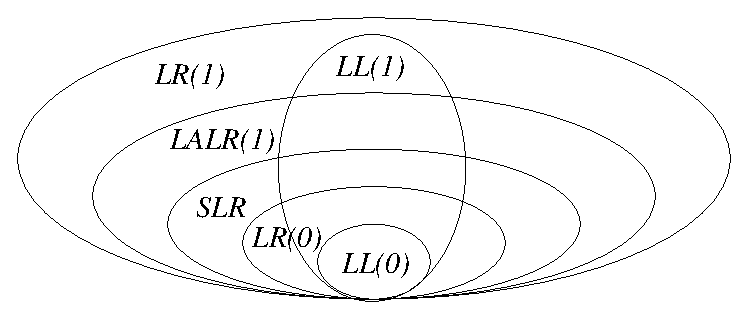
\epsfig{file = grammar_hierarchy.eps, width = 12cm}
\end{center}
\caption{La relazione fra le tecniche di parsing e le classi di grammatica
         considerate.}
  \label{fig:all_classes}
\end{figure}

Le tecniche di parsing $\mathit{LR}(0)$, $\mathit{LR}(1)$ ed
$\mathit{LALR}(1)$ si possono generalizzare a tecniche di parsing che
guardano fino a $k$ caratteri davanti alla testina di lettura dell'automa
a pila, con $k\ge 0$. Ne segue che esiste una \emph{gerarchia} di
tecniche di parsing (e conseguentemente di grammatiche da esse riconosciute).
\`E dimostrabile che ogni grammatica $\mathit{LL}(k)$ \`e anche
$\mathit{LR}(k)$, per ogni $k\ge 0$, e che il viceversa non \`e vero.
La Figura~\ref{fig:all_classes} mostra la relazione fra le classi
di parsing con $0\le k\le 1$. Si noti che $\mathit{LALR(0)}=\mathit{LR}(0)$.
Va osservato inoltre che tutte le classi di grammatica fin qui considerate
sono fatte da grammatiche non ambigue. Conseguentemente, nessuna tecnica di
parsing fra quelle viste sar\`a applicabile a una grammatica ambigua.
L'ambiguit\`a si traduce infatti in conflitti nella tabella
e solo una discesa ricorsiva non deterministica oppure
un automa a pila non deterministico potrebbero seguire al contempo
le annotazioni contrastanti della tabella. Ma tali tecniche sarebbero
troppo costose in termini computazionali.

Il parsing $\mathit{LALR}(1)$ \`e considerato come il metodo \emph{ideale} di
parsing, \nec troppo costoso \nec troppo impreciso. Per questo motivo esso
\`e implementato da JavaCup. Va detto che JavaCup costruisce
\emph{direttamente}
l'automa $\mathit{LALR}(1)$, senza passare per la semplificazione dell'automa
$\mathit{LR}(1)$, evitando quindi l'esplosione combinatoria degli stati per la
costruzione dell'automa intermedio $\mathit{LR}(1)$.
Non ci occupiamo comunque qui di questa ottimizzazione.

\`E importante invece discutere come si comporta JavaCup se nella
costruzione della tabella $\mathit{LALR}(1)$ vengono incontrari dei
conflitti, situazione non desiderabile ma che purtroppo si verifica
spesso in pratica. JavaCup usa in tal caso un sistema di \emph{risoluzione}
dei conflitti che consiste nello scegliere una delle annotazioni contrastanti
della tabella. Va subito osservato che una simile tecnica
in genere restringe l'insieme
degli alberi di parsing riconosciuti dall'automa e quindi pu\`o potenzialmente
cambiare il linguaggio da esso riconosciuto o forzare un'interpretazione
piuttosto che un'altra nel caso di grammatiche ambigue. Comunque sia,
JavaCup risolve i conflitti sposta/riduci in favore dello spostamento e i
conflitti riduci/riduci in favore della riduzione per la produzione che
appare prima nella grammatica.

JavaCup visualizza le scelte di risoluzione dei conflitti incontrati durante la generazione
di un parser, nella console di Eclipse oppure
nel file di log \texttt{resources/Kitten.err}, insieme agli stati dell'automa
$\mathit{LALR}(1)$ e alle relative transizioni. Tale informazione andrebbe quindi
sempre controllata dopo la generazione di un parser. \`E possibile specificare
un numero massimo di risoluzioni accettabili da JavaCup, superato il quale
la creazione del parser non \`e effettuata.
%
\subsection{Il parsing $\mathit{LR}$ con grammatiche ambigue}
  \label{subsec:ambiguity}
%
Abbiamo osservato che nessuna grammatica ambigua pu\`o essere
processata con uno dei metodi di parsing gi\`a visti. Abbiamo anche
detto che \`e spesso possibile trovare grammatiche non ambigue
equivalenti, ma che esse sono tipicamente complesse e innaturali
(Sezione~\ref{subsec:priorities}). In questa sezione riconsideriamo il
problema partendo dalla grammatica in Figura~\ref{fig:expressions_ambiguity}
che esprime in piccolo i problemi di ambiguit\`a della grammatica per le
espressioni Kitten vista nella Sezione~\ref{subsec:expressions_specification}.
La Figura~\ref{fig:ambiguity_automaton} mostra l'automa
$\mathit{LR}(1)$ per la grammatica in Figura~\ref{fig:expressions_ambiguity}.
Conseguentemente la sua tabella $\mathit{LR}(1)$ \`e la seguente, in cui
sono evidenti molti conflitti:
%
\begin{figure}[t]
\begin{align*}
  0)\ \ \ \ \ \,I &\to \mathit{exp}\ \mathtt{\$}\\
  1)\ \ \mathit{exp} &\to\mathit{exp}\ \mathtt{PLUS}\ \mathit{exp}\\
  2)\ \ \mathit{exp} &\to \mathit{exp}\ \mathtt{TIMES}\ \mathit{exp}\\
  3)\ \ \mathit{exp} &\to \mathtt{INTEGER}
\end{align*}
\caption{Una grammatica ambigua per le espressioni aritmetiche.}
  \label{fig:expressions_ambiguity}
\end{figure}
%
\begin{figure}[t]
\[
{\scriptsize
\xymatrix{
  \fbox{$\begin{array}{rlr}
    \mathit{exp}&\to\mathit{exp}\ \mathtt{TIMES}\ \mathit{exp}\idot &
      \{\mathtt{\$},\mathtt{PLUS},\mathtt{TIMES}\}\\
    \mathit{exp}&\to\mathit{exp}\idot\ \mathtt{PLUS}\ \mathit{exp} &
      \{\mathtt{\$},\mathtt{PLUS},\mathtt{TIMES}\}\\
    \mathit{exp}&\to\mathit{exp}\idot\ \mathtt{TIMES}\ \mathit{exp} &
      \{\mathtt{\$},\mathtt{PLUS},\mathtt{TIMES}\}
  \end{array}$}^{\ 1}\ar@/_35ex/[ddd]_(.8){\mathtt{TIMES}}
    \ar@/^/[rd]^{\mathtt{PLUS}}
  \\
  \fbox{$\begin{array}{rlr}
    \mathit{exp}&\to\mathit{exp}\ \mathtt{PLUS}\ \mathit{exp}\idot &
      \{\mathtt{\$},\mathtt{PLUS},\mathtt{TIMES}\}\\
    \mathit{exp}&\to\mathit{exp}\idot\ \mathtt{PLUS}\ \mathit{exp} &
      \{\mathtt{\$},\mathtt{PLUS},\mathtt{TIMES}\}\\
    \mathit{exp}&\to\mathit{exp}\idot\ \mathtt{TIMES}\ \mathit{exp} &
      \{\mathtt{\$},\mathtt{PLUS},\mathtt{TIMES}\}
  \end{array}$}^{\ 2}\ar@/_22ex/[dd]^(.3){\mathtt{TIMES}}
    \ar@/^3ex/[r]^{\mathtt{PLUS}}
  &
  \fbox{$\begin{array}{rlr}
    \mathit{exp}&\to\mathit{exp}\ \mathtt{PLUS}\idot\ \mathit{exp} &
      \{\mathtt{\$},\mathtt{PLUS},\mathtt{TIMES}\}\\
    \mathit{exp}&\to\idot\mathit{exp}\ \mathtt{PLUS}\ \mathit{exp} &
      \{\mathtt{\$},\mathtt{PLUS},\mathtt{TIMES}\}\\
    \mathit{exp}&\to\idot\mathit{exp}\ \mathtt{TIMES}\ \mathit{exp} &
      \{\mathtt{\$},\mathtt{PLUS},\mathtt{TIMES}\}\\
    \mathit{exp}&\to\idot\mathtt{INTEGER} &
      \{\mathtt{\$},\mathtt{PLUS},\mathtt{TIMES}\}
  \end{array}$}^{\ 3}\ar@/^3ex/[l]^{\mathit{exp}}\ar@/^/[ld]_{\mathtt{INTEGER}}
  \\
  \fbox{$\begin{array}{rlr}
    \mathit{exp}&\to\mathtt{INTEGER}\idot &
      \{\mathtt{\$},\mathtt{PLUS},\mathtt{TIMES}\}
  \end{array}$}^{\ 4}
  &
  \fbox{$\begin{array}{rlr}
    I&\to\idot\mathit{exp}\ \mathtt{\$}\\
    \mathit{exp}&\to\idot\mathit{exp}\ \mathtt{PLUS}\ \mathit{exp} &
      \{\mathtt{\$},\mathtt{PLUS},\mathtt{TIMES}\}\\
    \mathit{exp}&\to\idot\mathit{exp}\ \mathtt{TIMES}\ \mathit{exp} &
      \{\mathtt{\$},\mathtt{PLUS},\mathtt{TIMES}\}\\
    \mathit{exp}&\to\idot\mathtt{INTEGER} &
      \{\mathtt{\$},\mathtt{PLUS},\mathtt{TIMES}\}
  \end{array}$}^{\ 0}\ar[l]^{\mathtt{INTEGER}}\ar[d]^{\mathit{exp}}
  \\
  \fbox{$\begin{array}{rlr}
    \mathit{exp}&\to\mathit{exp}\ \mathtt{TIMES}\idot\ \mathit{exp} &
      \{\mathtt{\$},\mathtt{PLUS},\mathtt{TIMES}\}\\
    \mathit{exp}&\to\idot\mathit{exp}\ \mathtt{PLUS}\ \mathit{exp} &
      \{\mathtt{\$},\mathtt{PLUS},\mathtt{TIMES}\}\\
    \mathit{exp}&\to\idot\mathit{exp}\ \mathtt{TIMES}\ \mathit{exp} &
      \{\mathtt{\$},\mathtt{PLUS},\mathtt{TIMES}\}\\
    \mathit{exp}&\to\idot\mathtt{INTEGER} &
      \{\mathtt{\$},\mathtt{PLUS},\mathtt{TIMES}\}
  \end{array}$}^{\ 5}\ar@/^31ex/[uuu]_(.5){\mathit{exp}}
    \ar[u]^{\mathtt{INTEGER}}
  &
  \fbox{$\begin{array}{rlr}
    I&\to\mathit{exp}\idot\ \mathtt{\$}\\
    \mathit{exp}&\to\mathit{exp}\idot\ \mathtt{PLUS}\ \mathit{exp} &
      \{\mathtt{\$},\mathtt{PLUS},\mathtt{TIMES}\}\\
    \mathit{exp}&\to\mathit{exp}\idot\ \mathtt{TIMES}\ \mathit{exp} &
      \{\mathtt{\$},\mathtt{PLUS},\mathtt{TIMES}\}
  \end{array}$}^{\ 6}\ar@/_26ex/[uu]_(.7){\mathtt{PLUS}}
    \ar[l]^{\mathtt{TIMES}}
}}
\]
\caption{L'automa $\mathit{LR}(1)$ per la grammatica in Figura~\ref{fig:expressions_ambiguity}.}\label{fig:ambiguity_automaton}
\end{figure}
%
\begin{equation}\label{tab:expressions_conflicts}
\begin{array}{c||c|c|c|c||c|c|}
  & \mathtt{\$} & \mathtt{PLUS} & \mathtt{TIMES} & \mathtt{INTEGER} & I  & \mathit{exp}\\\hline\hline
0 &             &     &     & s4   &    & g6 \\\hline
1 & r2          & s3/r2 & s5/r2 &      &    &    \\\hline
2 & r1          & s3/r1 & s5/r1 &      &    &    \\\hline
3 &             &     &     & s4   &    & g2 \\\hline
4 & r3          & r3  & r3  &      &    &    \\\hline
5 &             &     &     & s4   &    & g1 \\\hline
6 & a           & s3  & s5  &      &    &    \\\hline
\end{array}
\end{equation}

C'\`e un conflitto sposta/riduci
nello stato $1$, di fronte al token \texttt{PLUS}, poich\'e
possiamo sia spostarci nello stato $3$ che ridurre secondo la produzione
$\mathit{exp}\to\mathit{exp}\ \mathtt{TIMES}\ \mathit{exp}$. L'item
$\mathit{exp}\to\mathit{exp}\ \mathtt{TIMES}\ \mathit{exp}\idot$ nello
stato $1$ ci dice che in tale stato abbiamo finito di leggere dal file
sorgente qualcosa che \`e il prodotto di due espressioni $\mathit{exp}_1$
ed $\mathit{exp}_2$. Ridurre secondo
la produzione $\mathit{exp}\to\mathit{exp}\ \mathtt{TIMES}\ \mathit{exp}$
significherebbe quindi vedere tale prodotto come un'unica espressione il cui
risultato \`e sommato con quel che segue.
Spostare il token $\mathtt{PLUS}$ significherebbe considerare
$\mathit{exp}_2$ come l'inizio di una addizione, il cui risultato deve
essere poi moltiplicato per $\mathit{exp}_1$. \`E qui evidente che
ci scontriamo contro l'ambiguit\`a della grammatica. Ridurre secondo la
produzione $\mathit{exp}\to\mathit{exp}\ \mathtt{TIMES}\ \mathit{exp}$
significa dare priorit\`a alla moltiplicazione, mentre spostare
$\mathtt{PLUS}$ significa dare priorit\`a all'addizione. La scelta ragionevole
\`e quindi quella di risolvere l'ambiguit\`a riducendo secondo la produzione
$\mathit{exp}\to\mathit{exp}\ \mathtt{TIMES}\ \mathit{exp}$. In termini della
tabella $\mathit{LR}(1)$, questo significa che nello stato $1$, di fronte
a $\mathtt{PLUS}$, risolviamo il conflitto
lasciando l'azione di riduzione ed eliminado l'azione di spostamento del token.
Un ragionamento simile ci fa concludere che nello stato $2$,
di fronte al token $\mathtt{TIMES}$, preferiamo spostare il token
piuttosto che ridurre secondo la produzione
$\mathit{exp}\to\mathit{exp}\ \mathtt{PLUS}\ \mathit{exp}$.

Un altro conflitto sorge ancora nello stato $1$ di fronte al token
$\mathtt{TIMES}$. In tale stato abbiamo gi\`a letto dei token che formano
la moltiplicazione di due espressioni $\mathit{exp}_1$ ed $\mathit{exp}_2$.
Abbiamo sia la possibilit\`a di ridurre secondo la produzione
$\mathit{exp}\to\mathit{exp}\ \mathtt{TIMES}\ \mathit{exp}$ che
di spostare il token $\mathtt{TIMES}$
e andare nello stato $5$. La prima scelta significa
legare il prodotto di $\mathit{exp}_1$ ed $\mathit{exp}_2$
riducendolo a un'espressione moltiplicata per
quel che segue il $\mathtt{TIMES}$, mentre la seconda scelta considera
$\mathit{exp}_2$ come l'inizio di un prodotto il cui risultato
viene moltiplicato per $\mathit{exp}_1$. Dal momento che preferiamo una
associativit\`a a sinistra per la moltiplicazione, facciamo la scelta di
ridurre secondo la produzione
$\mathit{exp}\to\mathit{exp}\ \mathtt{TIMES}\ \mathit{exp}$.
Similmente nello stato $2$ di fronte al token $\mathtt{PLUS}$ preferiamo
ridurre secondo la produzione
$\mathit{exp}\to\mathit{exp}\ \mathtt{PLUS}\ \mathit{exp}$ piuttosto
che spostare e andare nello stato $3$. Ecco quindi che la
tabella~\eqref{tab:expressions_conflicts}
viene semplificata in una tabella senza conflitti:
%
\[
\begin{array}{c||c|c|c|c||c|c|}
  & \mathtt{\$} & \mathtt{PLUS} & \mathtt{TIMES} & \mathtt{INTEGER} & I  & \mathit{exp}\\\hline\hline
0 &             &     &     & s4   &    & g6 \\\hline
1 & r2          & r2 & r2 &      &    &    \\\hline
2 & r1          & r1 & s5 &      &    &    \\\hline
3 &             &     &     & s4   &    & g2 \\\hline
4 & r3          & r3  & r3  &      &    &    \\\hline
5 &             &     &     & s4   &    & g1 \\\hline
6 & a           & s3  & s5  &      &    &    \\\hline
\end{array}
\]
che implementa il parsing delle espressioni aritmetiche con le
usuali regole di precedenza e associativit\`a.

La specifica della precedenza e dell'associativit\`a degli operatori
aritmetici viene fatta in JavaCup con le direttive che abbiamo visto nella
Sezione~\ref{subsec:priorities}, le quali modificano il comportamento
di JavaCup nella risoluzione dei conflitti (Sezione~\ref{subsec:lalr1}).
Una direttiva \texttt{precedence xxx $t$} d\`a infatti al token $t$ una
priorit\`a maggiore di quella di tutti gli altri token enumerati da
direttive precedenti dello stesso genere. Inoltre essa d\`a alle produzioni, il cui ultimo
token a destra \`e $t$, una priorit\`a pari a quella di $t$. Un conflitto
sposta/riduci viene a questo punto risolto preferendo lo spostamento se il
token spostato ha priorit\`a maggiore della produzione per cui si dovrebbe
ridurre; preferendo la riduzione nel caso opposto. Conseguentemente, con le direttive
della Sezione~\ref{subsec:priorities}, fra una riduzione per
$\mathit{exp}\to\mathit{exp}\ \mathtt{TIMES}\ \mathit{exp}$ e lo spostamento
di un $\mathtt{PLUS}$ si preferisce la riduzione. A parit\`a di
priorit\`a si seguono le direttive di associativit\`a preferendo la
riduzione se l'associativit\`a \`e \texttt{left}, lo spostamento
se l'associativit\`a \`e \texttt{right} e lasciando la casella vuota
se l'associativit\`a \`e \texttt{nonassoc}, in modo da segnalare un errore
in tale situazione.

Un altro problema di ambiguit\`a della grammatica Kitten (e in genere di
tutti i linguaggi imperativi) \`e relativo
all'\texttt{if/then/else}, in cui il ramo \texttt{else} \`e normalmente
facoltativo. Ne consegue che nel caso di \texttt{if} annidati risulta ambigua
l'associazione degli \texttt{else} all'\texttt{if} da cui dipendono.
Questo problema \`e tipicamente risolto associando
ogni \texttt{else} all'ultimo \texttt{then} incontrato. Per esempio,
vogliamo che
\texttt{if (a > 5) then if (b < 4) then a := 3 else b := 6}
venga interpretato come
\texttt{if (a > 5) then \{if (b < 4) then a := 3 else b := 6\}}
piuttosto che come
\texttt{if (a > 5) then \{if (b < 4) then a := 3\} else b := 6}.
A tal fine il parser, di fronte all'ultimo token \texttt{ELSE},
deve spostare tale token piuttosto che ridurre secondo la produzione
%
\begin{verbatim}
  exp ::= IF LPAREN exp RPAREN THEN command
\end{verbatim}
%
della Sezione~\ref{subsec:commands_specification}.
Abbiamo detto nella Sezione~\ref{subsec:lalr1} che
JavaCup risolve un conflitto sposta/riduci in favore dello spostamento,
che \`e quello che volevamo, e segnalando su console o annotando nel
file \texttt{resources/Kitten.err} che il conflitto \`e stato risolto in
tal senso. Per evitare tale annotazione (essenzialmente un \emph{warning})
e non contare questa risoluzione nel novero di quelle ammesse al massimo
da JavaCup, basta dichiarare esplicitamente che l'\texttt{ELSE} ha priorit\`a
rispetto al \texttt{THEN}. Otteniamo questo effetto aggiungendo al file
\texttt{resources/Kitten.cup} le dichiarazioni:
%
\begin{verbatim}
  precedence nonassoc THEN;
  precedence nonassoc ELSE;
\end{verbatim}
%
la cui annotazione di associativit\`a \`e irrilevante.
Un simile problema si presenta fra gli operatori di confronto e i token
\texttt{DOT} e \texttt{LBRACK}, risolto in modo simile (si veda la
Sezione~\ref{subsec:priorities}).

Un altro problema di ambiguit\`a della grammatica Kitten della
Sezione~\ref{sec:java_cup} \`e legato al meno unario. L'espressione
$\mathtt{MINUS}\ \mathit{exp}\ \mathtt{PLUS}\ \mathit{exp}$ pu\`o
essere interpretata sia come
$\mathtt{MINUS}\ (\mathit{exp}\ \mathtt{PLUS}\ \mathit{exp})$ che come
$(\mathtt{MINUS}\ \mathit{exp})\ \mathtt{PLUS}\ \mathit{exp}$ e quest'ultima
\`e l'interpretazione preferita. Conseguentemente la riduzione
secondo la produzione \texttt{exp ::= MINUS exp} deve essere preferita
a qualsiasi spostamento dei token che seguono la prima espressione.
Otteniamo questo effetto dando esplicitamente una priorit\`a massima a tale
produzione:
%
\begin{verbatim}
  exp ::= MINUS exp %prec UMINUS
\end{verbatim}
%
dove il token \texttt{UMINUS} ha ricevuto una priorit\`a maggiore di qualsiasi
suo seguito (Sezione~\ref{subsec:priorities}).

Risolti questi aspetti di ambiguit\`a della grammatica Kitten, il
programma JavaCup \`e capace di generare il parser per Kitten senza
segnalare alcuna risoluzione di conflitto.

Concludiamo questa sezione ricordando che la risoluzione dei conflitti
tramite annotazioni di precedenza e associativit\`a \`e generalmente
pericolosa perch\'e si rischia di cambiare il linguaggio riconosciuto dal
parser. Essa \`e usata in letteratura limitatamente ai soli esempi visti in
questa sezione.
%
\section{Le azioni semantiche e la costruzione induttiva della sintassi astratta}\label{sec:abstract_syntax}
%
La grammatica Kitten della Sezione~\ref{sec:java_cup} specifica
quali stringhe (\emph{file sorgenti}) appartengono al linguaggio Kitten.
Il parser generato da JavaCup si limita quindi a riconoscere le stringhe
del linguaggio. JavaCup ammette per\`o la possibilit\`a di \emph{decorare}
la grammatica con delle \emph{azioni semantiche} che vengono eseguite
in corrispondenza alle azioni di riduzione della tabella $\mathit{LALR}(1)$.
Tali azioni semantiche possono essere usate per molti scopi. In questa
sezione vediamo alcuni esempi.

Riconsideriamo la grammatica in Figura~\ref{fig:grammar_lists}, che in
JavaCup \`e scritta come
%
\begin{verbatim}
  terminal a b;
  non terminal L A B;

  start with L;

  L ::= A B ;
  A ::=
   | a A ;
  B ::=
   | b B ;
\end{verbatim}
%
Supponiamo di voler sapere, per ogni file sorgente, non solo se esso
soddisfa la grammatica, cio\`e se esso \`e formato da una lista di
\texttt{a} seguita da una lista di \texttt{b}, ma anche la lunghezza delle
due liste. A tal fine decidiamo che il non terminale $A$ deve conoscere
quante \texttt{a} sono state derivate da esso e il non terminale $B$
quante \texttt{b} sono state derivate da esso. Diciamo che il
\emph{valore semantico} del non terminale $A$ \`e il numero di \texttt{a}
da esso derivate e il valore semantico del non terminale $B$ \`e il numero
di \texttt{b} da esso derivate. I valori semantici vanno dichiarati nella
enumerazione dei non terminali. Dal momento che nel nostro caso si tratta
di valori interi, scriveremo\footnote{Il valore semantico in JavaCup deve
in effetti essere un oggetto, per cui non \`e possibile utilizzare il tipo
primitivo \texttt{int} ma occorrerebbe far ricorso alla classe involucro
\texttt{java.lang.Integer}. \`E solo per semplicit\`a espositiva che preferiamo
utilizzare nei nostri esempi il tipo \texttt{int}.}
%
\begin{verbatim}
  non terminal int A;
  non terminal int B;
\end{verbatim}
%
A questo punto dobbiamo specificare come si calcolano tali valori semantici.
Il calcolo avviene
\emph{decorando} ciascuna produzione per $A$ con delle \emph{azioni semantiche}
che specificano il valore semantico di $A$ per ciascuna delle sue due
produzioni. Similmente per $B$:
%
\begin{verbatim}
  A ::=
     {: RESULT = 0; :}
   | a A:l
     {: RESULT = 1 + l; :} ;

  B ::=
     {: RESULT = 0; :}
   | b B:l
     {: RESULT = 1 + l; :} ;
\end{verbatim}
%
Le azioni semantiche sono codice Java che si aggiunge dopo ciascuna produzione,
racchiuso fra i delimitatori \verb!{:! e \verb!:}!. Tale codice calcola
il valore semantico \texttt{RESULT} usando i valori semantici dei componenti
dei lati destri delle produzioni. Nell'esempio sopra diciamo che se una
lista di \texttt{a} \`e vuota allora il numero di \texttt{a}
incontrate \`e $0$. Se una lista di \texttt{a} \`e invece fatta da una
\texttt{a} seguita da $l$ \texttt{a}, il numero complessivo di \texttt{a}
incontrate \`e $1 + l$. Un ragionamento simile si applica per $B$.
Si noti che abbiamo \emph{decorato} dei non terminali alla destra delle
produzioni facendoli seguire da un carattere due punti e da una variabile
che contiene il loro valore semantico. \`E possibile decorare anche i terminali
che stanno alla destra di una produzione. Il valore semantico dei terminali
\`e per definizione il loro valore lessicale (Capitolo~\ref{chap:lexical})
che normalmente \`e \texttt{null} tranne se l'analizzatore lessicale
ha sintettizato per essi un apposito valore lessicale, come avviene in Kitten
per gli identificatori, le stringhe e le costanti numeriche.

Continuando il nostro esempio, il numero di \texttt{a} e il numero di
\texttt{b} incontrate nel file sorgente vanno fatti risalire fino al
non terminale iniziale. Dal momento che si tratta di \emph{due} interi,
siamo costretti a definire una struttura dati composta da due campi
di tipo \texttt{int}:
%
\begin{verbatim}
  public class Pair {
    private int a;
    private int b;

    public Pair(int a, int b) {
      this.a = a;
      this.b = b;
    }
  }
\end{verbatim}
%
Dichiariamo il tipo del valore lessicale per la $L$:
%
\begin{verbatim}
  non terminal Pair L;
\end{verbatim}
%
quindi specifichiamo come si costruisce tale valore lessicale:
%
\begin{verbatim}
  L ::= A:a B:b
      {: RESULT = new Pair(a,b); :} ;
\end{verbatim}
%
La grammatica decorata \`e in Figura~\ref{fig:grammar_lists_decoration}.
Il valore semantico del non terminale iniziale \`e poi ritornato
come valore di ritorno del metodo \texttt{parse()} della classe
\texttt{Parser} che viene generata da JavaCup
(Sezione~\ref{subsec:jlex_and_java_cup}).
%
\begin{figure}[t]
\begin{verbatim}
                       terminal a b;
                       non terminal int A;
                       non terminal int B;
                       non terminal Pair L;
                       start with L;

                       L ::= A:a B:b
                            {: RESULT = new Pair(a,b); :} ;

                       A ::=
                            {: RESULT = 0; :}
                         | a A:l
                            {: RESULT = 1 + l; :} ;

                       B ::=
                            {: RESULT = 0; :}
                         | b B:l
                            {: RESULT = 1 + l; :} ;
\end{verbatim}
\caption{La grammatica di Figura~\ref{fig:grammar_lists} decorata con delle
         azioni semantiche che calcolano il numero di \texttt{a} e il numero
         di \texttt{b} incontrate nel file sorgente.}
  \label{fig:grammar_lists_decoration}
\end{figure}

L'implementaziome delle azioni semantiche \`e basata su una semplice
modifica dell'automa a pila della Sezione~\ref{sec:lr}. Oltre a utilizzare
uno stack di stati, l'automa a pila utilizza adesso anche uno stack di
valori semantici, corrispondenti ai terminali o non terminali che sono
stati spostati o a cui si \`e ridotto per ottenere lo stato
nella posizione corrispondente dello stack di stati.
Tale stack di valori semantici \`e in effetti implementato da JavaCup come
uno stack di \texttt{java\_cup.runtime.Symbol}
(Figura~\ref{fig:java_cup.runtime.Symbol}). Il campo \texttt{value} \`e
utilizzato proprio per contenere il valore semantico ed \`e accessibile
tramite la variabile $v$ che si dichiara nella notazione
$\mathit{terminale}:v$ o $\mathit{non\ terminale}:v$.

Simuliamo per esempio
il comportamento dell'automa a pila di fronte alla stringa
$\mathtt{aab\$}$, utilizzando la tabella~\eqref{tab:slr_grammar_lists} e le
azioni semantiche in Figura~\ref{fig:grammar_lists_decoration}.
Indicando con $/$ il valore semantico $\mathtt{null}$, la
configurazione iniziale dell'automa \`e:
%
\begin{align*}
  0 & & \mathtt{aab\$}\\
  / & &
\end{align*}
%
dove il valore semantico $/$ per lo stato $0$ \`e irrilevante. A questo
punto, di fronte al lookahead \texttt{a}, la
tabella~\eqref{tab:slr_grammar_lists} ci dice di andare nello stato $2$.
Dal momento che il valore semantico dei token \`e per default
$\mathtt{null}$, otteniamo la configurazione
%
\begin{align*}
  0,2 & & \mathtt{ab\$}\\
  /,/ & &
\end{align*}
%
Nello stato $2$ di fronte al lookahead \texttt{a} restiamo in $2$:
%
\begin{align*}
  0,2,2 & & \mathtt{b\$}\\
  /,/,/ & &
\end{align*}
%
mentre di fronte al lookahead \texttt{b} riduciamo secondo la
produzione $A\to\varepsilon$ e poi andiamo nello stato $5$.
La produzione \`e stata decorata in modo tale che il
valore semantico della $A$ \`e $0$. La configurazione risultante \`e quindi:
%
\begin{align*}
  0,2,2,5 & & \mathtt{b\$}\\
  /,/,/,0 & &
\end{align*}
%
Nello stato $5$ di fronte al lookahead \texttt{b} riduciamo secondo
la produzione $A\to\mathtt{a}A$ per cui dobbiamo levare due stati dallo
stack e sostituirli con lo stato $5$. Gli ultimi due elementi dello stack
dei valori semantici sono $/$ e $0$ per cui nella
Figura~\ref{fig:grammar_lists_decoration} il valore di $l$ \`e $0$.
Conseguentemente il valore semantico $1+l$ \`e pari ad $1$ e otteniamo la
configurazione:
%
\begin{align*}
  0,2,5 & & \mathtt{b\$}\\
  /,/,1 & &
\end{align*}
%
Dobbiamo nuovamente ridurre secondo la produzione $A\to\mathtt{a}A$ ottenendo
questa volta:
%
\begin{align*}
  0,3 & & \mathtt{b\$}\\
  /,2 & &
\end{align*}
%
Nello stato $3$ di fronte al lookahead \texttt{b} finiamo nello stato $6$:
%
\begin{align*}
  0,3,6 & & \mathtt{\$}\\
  /,2,/ & &
\end{align*}
%
e nello stato $6$ di fronte al lookahead $\mathtt{\$}$ riduciamo secondo la
produzione $B\to\varepsilon$ per cui otteniamo la configurazione
%
\begin{align*}
  0,3,6,7 & & \mathtt{\$}\\
  /,2,/,0 & &
\end{align*}
%
Nello stato $7$ di fronte al lookahead $\mathtt{\$}$ riduciamo secondo la
produzione $B\to\mathtt{b}B$ per cui dobbiamo eliminare due stati dallo stack
e sostituirli con lo stato $4$. Inoltre avremo $l=0$ in
Figura~\ref{fig:grammar_lists_decoration} e conseguentemente otteniamo la
configurazione:
%
\begin{align*}
  0,3,4 & & \mathtt{\$}\\
  /,2,1 & &
\end{align*}
%
Nello stato $4$ di fronte al lookahead $\mathtt{\$}$ dobbiamo ridurre
secondo la produzione $L\to AB$ per cui dobbiamo eliminare due
stati dallo stack e sostituirli con lo stato $1$. In
Figura~\ref{fig:grammar_lists_decoration} avremo $a=2$ e $b=1$ per cui
otteniamo la configurazione
%
\begin{align*}
  0,1 & & \mathtt{\$}\\
  /,p & &
\end{align*}
%
dove $p$ \`e un puntatore in memoria a un oggetto \texttt{Pair} i cui campi
\texttt{a} e \texttt{b} contengono rispettivamente $2$ e $1$.
A questo punto l'automa si ferma accettando la stringa $\mathtt{aab\$}$
poich\'e nello stato $1$ di fronte al lookahead $\mathtt{\$}$ la
tabella~\ref{tab:slr_grammar_lists} richiede di accettare il file sorgente.

Consideriamo un altro esempio di decorazione di una grammatica
con azioni semantiche. La grammatica in
Figura~\ref{fig:expressions_ambiguity} specifica delle espressioni aritmetiche
su interi. Supponiamo che l'analizzatore lessicale associ al token
\texttt{INTEGER} il valore numerico concreto presente nel file
sorgente (Capitolo~\ref{chap:lexical}). Le azioni semantiche in
Figura~\ref{fig:expressions_decoration} calcolano il valore dell'espressione
contenuta nel file sorgente. Si noti che se l'espressione \`e formata
semplicemente da un numero intero allora la produzione decorata
%
\begin{verbatim}
  exp ::= INTEGER:i
       {: RESULT = i; :} ;
\end{verbatim}
%
usa il valore lessicale del token \texttt{INTEGER} per sintetizzare il
valore semantico di \texttt{exp}. In tal caso occorre dichiarare
qual \`e il valore lessicale di \texttt{INTEGER}, con la dichiarazione
%
\begin{verbatim}
  terminal int INTEGER;
\end{verbatim}
%
Tale dichiarazione deve essere compatibile con il tipo del valore
lessicale effettivamente calcolato dall'analizzatore lessicale per il token
\texttt{INTEGER}.

\begin{figure}[t]
\begin{verbatim}
                       terminal PLUS, TIMES;
                       terminal int INTEGER;
                       non terminal int exp;
                       start with exp;

                       exp ::=
                           exp:e1 PLUS exp:e2
                             {: RESULT = e1 + e2; :}
                         | exp:e1 TIMES exp:e2
                             {: RESULT = e1 * e2; :}
                         | INTEGER:i
                             {: RESULT = i; :} ;
\end{verbatim}
\caption{La grammatica di Figura~\ref{fig:expressions_ambiguity}
         decorata con delle
         azioni semantiche che calcolano il valore dell'espressione di cui
         il file sorgente \`e composto.}
  \label{fig:expressions_decoration}
\end{figure}

\begin{exercise}\label{ex:decoration1}
Si scriva una grammatica non ambigua che genera il linguaggio delle
stringhe di \texttt{a} e \texttt{b}. Quindi la si decori con delle
azioni semantiche che calcolano la differenza fra il numero delle \texttt{a}
e il numero delle \texttt{b}.
\end{exercise}
%
\begin{exercise}\label{ex:decoration2}
Supponendo che il token \texttt{INTEGER} rappresenti solo numeri interi
maggiori o uguali a $0$, si decori la grammatica della
Figura~\ref{fig:expressions_ambiguity} con delle azioni semantiche che
calcolano un valore booleano. Tale valore deve essere \textit{true}
se e solo se il valore dell'espressione non \`e $0$.
\end{exercise}

Un'applicazione delle azioni semantiche \`e la creazione, durante il
parsing, della \emph{sintassi astratta}
del codice sorgente, cio\`e di un albero,
come quello della Figura~\ref{fig:led_albero}, che descrive la \emph{struttura
logica} del codice. L'idea \`e quella di fare
sintetizzare a ciascun non terminale, come valore semantico, la sintassi
astratta della parte di codice da esso derivata.

\begin{figure}[t]
\begin{verbatim}
                       terminal a b;
                       non terminal AbstractA A;
                       non terminal AbstractB B;
                       non terminal AB L;
                       start with L;

                       L ::= A:a B:b
                            {: RESULT = new AB(a,b); :} ;

                       A ::=
                            {: RESULT = new EmptyA(); :}
                         | a A:l
                            {: RESULT = new OneA(l); :} ;

                       B ::=
                            {: RESULT = new EmptyB(); :}
                         | b B:l
                            {: RESULT = new OneB(l); :} ;
\end{verbatim}
\caption{La grammatica di Figura~\ref{fig:grammar_lists} decorata con delle
         azioni semantiche che sintetizzano la sua sintassi astratta.}
  \label{fig:grammar_lists_abstract_syntax}
\end{figure}

Supponiamo per esempio di volere generare la sintassi astratta per la
grammatica in Figura~\ref{fig:grammar_lists}, modificando le azioni semantiche
della Figura~\ref{fig:grammar_lists_decoration}. Otteniamo la grammatica
decorata in Figura~\ref{fig:grammar_lists_abstract_syntax}.
La classe \texttt{EmptyB} rappresenta una sequenza vuota di \texttt{b}.
La classe \texttt{OneB} rappresenta invece una \texttt{b} seguita da una
sequenza di \texttt{b}. Dal momento che dobbiamo assegnare \emph{un} tipo
al valore semantico sintetizzato per \texttt{B}, tali due classi devono
essere sottoclassi di una classe \texttt{AbstractB} che denota
genericamente delle sequenze di \texttt{b}. Tale classe \`e bene che
sia lasciata astratta, nel senso di Java:
%
\begin{verbatim}
  public abstract class AbstractB {}

  public class EmptyB extends AbstractB {}

  public class OneB extends AbstractB {
    private AbstractB l;
    public OneB(AbstractB l) { this.l = l; }
  }
\end{verbatim}
%
Identica \`e l'impostazione delle classi \texttt{EmptyA},
\texttt{OneA} e \texttt{AbstractA}. La classe \texttt{AB} \`e invece definita
come:
%
\begin{verbatim}
  public class AB {
    private AbstractA a;
    private AbstractB b;
    public AB(AbstractA a, AbstractB b) { this.a = a; this.b = b; }
  }
\end{verbatim}
%
dal momento che c'\`e solo una produzione per \texttt{L}.

Si noti l'estrema \emph{arbitrariet\`a} della rappresentazione
della sintassi astratta. Per esempio, un'altra possibile organizzazione
della sintassi astratta per la grammatica in Figura~\ref{fig:grammar_lists}
\`e mostrata in Figura~\ref{fig:grammar_lists_abstract_syntax2}.
Questa volta le classi di sintassi astratta sono implementate come
%
\begin{verbatim}
  public class ListA {
    private ListA tail;
    public ListA(ListA tail) { this.tail = tail; }
  }

  public class ListB {
    private ListB tail;
    public ListB(ListB tail) { this.tail = tail; }
  }

  public class AB {
    private ListA a;
    private ListB b;
    public AB(ListA a, ListB b) { this.a = a; this.b = b; }
  }
\end{verbatim}

Altre scelte sarebbero possibili e legittime. In genere \`e importante
che la sintassi astratta semplifichi la comprensione e l'elaborazione
del codice che essa astrae (Capitolo~\ref{chap:recursive_descent}).
Una buona euristica \`e quella di definire una classe di sintassi astratta
per ogni produzione, i cui oggetti hanno un campo per ogni non terminale
nel lato destro della produzione. Quindi si definisce una classe astratta
(nel senso di Java) che fa da superclasse a tutte le classi di sintassi
astratta per le produzioni che hanno a sinistra lo stesso non terminale. Da
questo punto di vista \`e quindi
pi\`u \emph{standard} una sintassi astratta generata come in
Figura~\ref{fig:grammar_lists_abstract_syntax} che non una generata come in
Figura~\ref{fig:grammar_lists_abstract_syntax2}.
%
\begin{figure}[t]
\begin{verbatim}
                       terminal a b;
                       non terminal ListA A;
                       non terminal ListB B;
                       non terminal AB L;
                       start with L;

                       L ::= A:a B:b
                            {: RESULT = new AB(a,b); :} ;

                       A ::=
                            {: RESULT = null; :}
                         | a A:l
                            {: RESULT = new ListA(l); :} ;

                       B ::=
                            {: RESULT = null; :}
                         | b B:l
                            {: RESULT = new ListB(l); :} ;
\end{verbatim}
\caption{La grammatica di Figura~\ref{fig:grammar_lists} decorata con delle
         azioni semantiche che sintetizzano la sua sintassi astratta
         come liste di \texttt{a} e di \texttt{b}.}
  \label{fig:grammar_lists_abstract_syntax2}
\end{figure}

\greycomment{Le azioni semantiche possono essere utilizzate per svariati
scopi. L'unico uso per cui le utilizziamo nel compilatore Kitten \`e per la
generazione della sintassi astratta del codice sorgente. Su tale sintassi
astratta definiamo poi dei metodi virtuali a discesa ricorsiva
che permettono per esempio
di effettuare il type-checking e la generazione del codice intermedio
(Capitoli~\ref{chap:semantical} e~\ref{chap:translate}). \`E possibile
comunque utilizzare le stesse azioni semantiche per svolgere
tali compiti. Questo approccio \e sicuramente pi\`u
tradizionale~\cite{AhoSU86} ma finisce per sovraccaricare il file
\texttt{resources/Kitten.cup} con informazione non relativa all'aspetto
sintattico
del linguaggio. Inoltre l'uso di un linguaggio a oggetti per l'implementazione
del compilatore ben si accompagna alla definizione del type-checking e della
generazione del codice intermedio tramite metodi virtuali delle classi di
sintassi astratta, permettendo per esempio di definire in maniera molto
semplice un comportamento di default per tutta una classe di strutture
sintattiche (come per gli operatori binari).}
%
\section{La sintassi astratta di Kitten}\label{sec:abstract_syntax_classes}
%
La generazione della sintassi astratta di Kitten avviene come abbiamo
visto sopra in Figura~\ref{fig:grammar_lists_abstract_syntax}.
L'idea \`e di far sintetizzare a ciascun non terminale, tramite azioni
semantiche, l'albero di sintassi astratta della parte di codice
sorgente da esso derivato.

Vediamo per esempio come modifichiamo a tal fine una delle produzioni
della Sezione~\ref{subsec:expressions_specification}:
%
\begin{verbatim}
  exp ::= exp:left PLUS:p exp:right
     {: RESULT = new Addition(pleft,left,right); :}
\end{verbatim}
%
Per induzione, \texttt{left} e \texttt{right} contengono l'albero
di sintassi astratta per la parte di codice derivata dai due addendi
dell'addizione. Invece \texttt{p} contiene il valore lessicale del
token \texttt{PLUS}, che come abbiamo gi\`a detto \`e \texttt{null}
essendo \texttt{PLUS} un terminale. Questo non significa che
la notazione \texttt{PLUS:p} sia inutile: essa dichiara implicitamente
anche una variabile \texttt{pleft} che dice quanti caratteri sono
passati dall'inizio del file sorgente fino al token \texttt{PLUS}. In pratica,
\texttt{pleft} \`e un accesso al campo \texttt{left} della struttura
dati in Figura~\ref{fig:java_cup.runtime.Symbol}.
Conservare questa informazione nell'albero astratto \`e importante nel caso
in cui, in futuro, servisse segnalare un qualche errore su questa
addizione (Capitolo~\ref{chap:lexical}).
Si noti che esistono anche le variabili \texttt{leftleft} corrispondente
a \texttt{left} e \texttt{rightleft} corrispondente a \texttt{right}, ma
in questo caso esse non sono utilizzate. Quello che stiamo
dicendo con la precedente produzione \`e quindi
che il valore semantico per una addizione \`e un
albero astratto con una radice che \`e un nodo di tipo \texttt{Addition}
e i cui due figli sono gli alberi astratti per i due addendi dell'addizione.
Inoltre la posizione in cui deve essere segnalato un eventuale errore
semantico \`e quella del token \texttt{PLUS}.

Affich\'e la definizione induttiva dell'albero astratto per un pezzo di codice
sia ben fondata, occorre che ci siano anche dei casi base. Per esempio,
un caso base \`e il seguente:
%
\begin{verbatim}
  exp ::= TRUE:t
     {: RESULT = new True(tleft); :}
\end{verbatim}
%
il quale dice che il valore semantico per la costante \texttt{true}
\`e un nodo di tipo \texttt{True}, privo di figli. Eventuali
errori su questa parte di codice devono essere in futuro segnalati
alla posizione in cui inizia l'espressione \texttt{true}, cio\`e a
\texttt{tleft} caratteri dall'inizio del file sorgente.

Le classi di sintassi astratta utilizzate
per rappresentare il codice sorgente Kitten in maniera strutturata si trovano
all'interno della directory \texttt{absyn} di Kitten.
Esse sono tutte sottoclassi della classe astratta
(nel senso di Java) \texttt{absyn/Absyn.java} mostrata in
Figura~\ref{fig:absyn.Absyn}.
Una classe di sintassi astratta ha sempre un campo \texttt{pos} che
indica dove deve essere segnalato un errore verificatosi sulla parte di codice
da essa rappresentata. La posizione \texttt{pos} viene specificata
al momento della creazione del nodo di sintassi astratta tramite le azioni
semantiche e pu\`o essere letta in seguito con il metodo \texttt{getPos()}.
Si noti che ogni nodo di sintassi
astratta ha anche un identificatore numerico unico \texttt{identifier},
la cui utilit\`a sar\`a chiara in seguito quando descriveremo la
rappresentazione grafica dell'albero di sintassi astratta
(Sezione~\ref{sec:graphical_abstract_syntax}).
%
\begin{figure}[t]
\begin{verbatim}
                     public abstract class Absyn {
                       private int pos;
                       private int identifier;
                       private static int counter = 0;

                       protected Absyn(int pos) {
                         this.pos = pos;
                         this.identifier = counter++;
                       }

                       public int getPos() {
                         return pos;
                       }
                     }
\end{verbatim}
\caption{La superclasse di tutte le classi di sintassi astratta per Kitten.}
  \label{fig:absyn.Absyn}
\end{figure}

Le espressioni sono una sottoclasse di \texttt{absyn/Absyn.java}.
Le definiamo come
%
\begin{verbatim}
  public abstract class Expression extends Absyn {
    protected Expression(int pos) {
      super(pos);
    }
  }
\end{verbatim}
%
A questo punto possiamo dire che la classe di sintassi astratta
\texttt{absyn/True.java} \`e un caso particolare di espressione:
%
\begin{verbatim}
  public class True extends Expression {
    public True(int pos) {
      super(pos);
    }
  }
\end{verbatim}
%
Si noti che questa volta si tratta di una classe concreta, nel senso di Java.

Il caso della classe di sintassi astratta \texttt{absyn/Addition.java}, che
rappresenta un'operazione binaria di addizione, \`e
pi\`u complesso. In primo luogo, definiamo le operazioni binarie come un
caso particolare delle espressioni:
%
\begin{verbatim}
  public abstract class BinOp extends Expression {
    private Expression left;
    private Expression right;

    protected BinOp(int pos, Expression left, Expression right) {
      super(pos);
      this.left = left;
      this.right = right;
    }
  }
\end{verbatim}
%
Si noti che un'operazione binaria ha due campi \texttt{left} e \texttt{right}
che sono, ricorsivamente, la sintassi astratta dei suoi due operandi.
Si noti inoltre che il costruttore inizializza la parte di stato di sua
competenza e demanda alla superclasse l'inizializzazione del resto, cio\`e in
questo caso di \texttt{pos}.
A questo punto definiamo un caso particolare di operazione binaria,
cio\`e un'operazione binaria aritmetica:
%
\begin{verbatim}
  public abstract class ArithmeticBinOp extends BinOp {
    protected ArithmeticBinOp(int pos, Expression left, Expression right) {
      super(pos,left,right);
    }
  }
\end{verbatim}
%
Siamo finalmente nelle condizioni di definire \texttt{absyn/Addition.java}
come un caso particolare di operazione binaria aritmetica:
%
\begin{verbatim}
  public class Addition extends ArithmeticBinOp {
    public Addition(int pos, Expression left, Expression right) {
      super(pos,left,right);
    }
  }
\end{verbatim}
%
Questa volta si tratta di una classe concreta, nel senso di Java.
Si osservi che le classi
astratte, nel senso di Java, hanno costruttori \texttt{protected},
utilizzabili quindi solo dalle classi concrete che le estendono,
tramite la chiamata \texttt{super} a un costruttore della superclasse.

\javatip{
La strutturazione gerarchica delle classi di sintassi astratta e l'uso
intenso di classi astratte, nel senso di Java, pu\`o non essere immediatamente
apprezzabile. Quando, per\`o, definiremo algoritmi ricorsivi sulla sintassi
astratta, ci accorgeremo che una buona strutturazione gerachica aiuta
significativamente la definizione di tali algoritmi. \`E un tipico
caso in cui l'impostazione a oggetti del codice semplifica
nettamente lo sviluppo del software.}

Vediamo adesso in maniera pi\`u dettagliata quali sono le classi di
sintassi astratta di Kitten.
%
\subsection{Le classi di sintassi astratta per i tipi}
  \label{subsec:types_abstract}
%
\begin{figure}[t]
\begin{center}
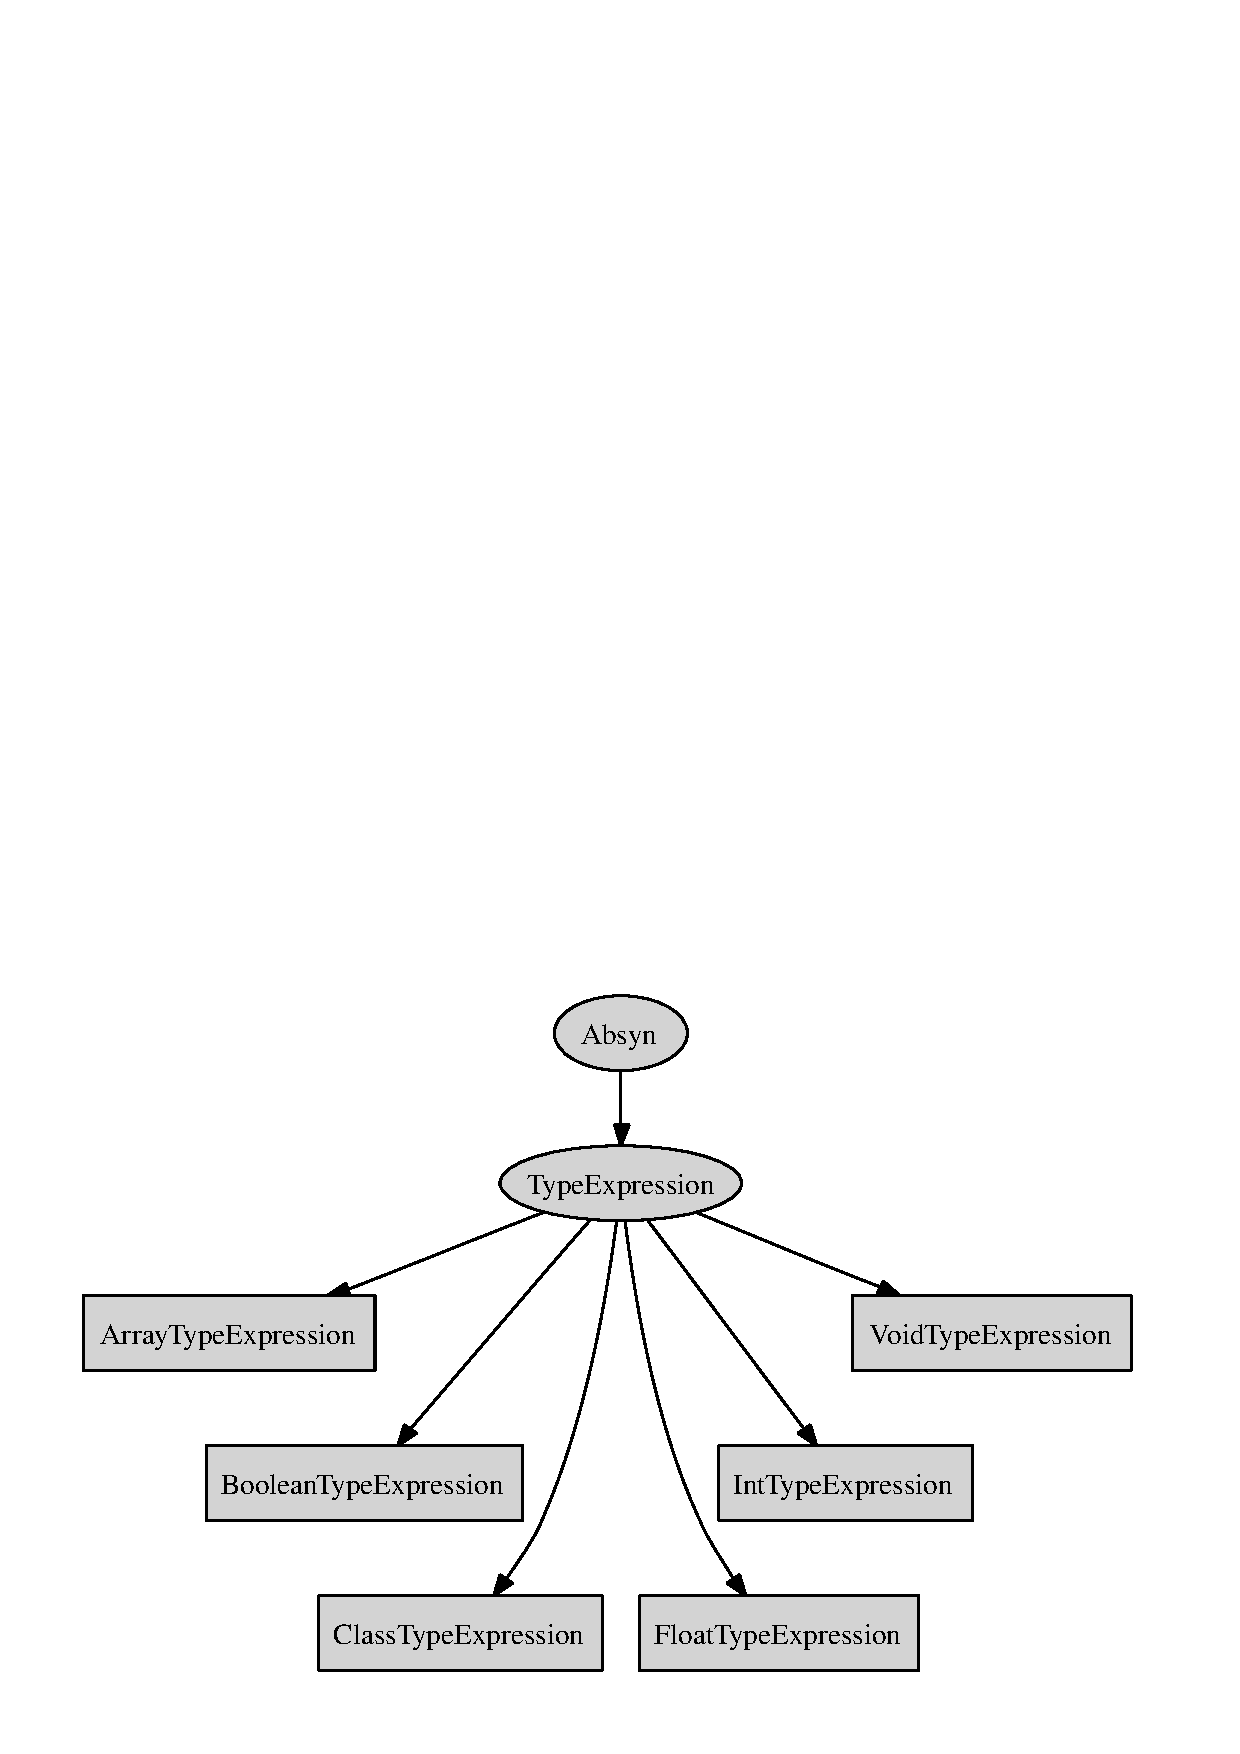
\epsfig{file = types_hierarchy.pdf, width = 14cm}
\end{center}
\caption{La struttura gerarchica delle classi di sintassi astratta per
         i tipi. Le classi astratte sono indicate con un
         ovale, quelle concrete con un rettangolo.}
  \label{fig:types_hierarchy}
\end{figure}

\begin{figure}[t]
\begin{verbatim}
  public class Symbol implements Comparable {
    // alcuni simboli usati di frequente
    public static final Symbol THIS = mk("this");
    public static final Symbol OBJECT = mk("Object");
    public static final Symbol STRING = mk("String");
    private String name;   // il nome del simbolo

    private Symbol(String name) { // si noti: e' private!
      this.name = name;
    }

    // possiamo creare simboli solo con questo metodo
    public static Symbol mk(String name) {
      // usa una tabella statica per determinare se il simbolo e' gia'
      // stato creato e in tal caso lo ritorna. Altrimenti lo crea,
      // lo aggiunge alla tabella e lo ritorna
    }

    public String toString() { return name; }

    public int compareTo(Object other) {
      if (!(other instanceof Symbol)) return 0;
      return name.compareTo(((Symbol)other).name);
    }
  }
\end{verbatim}
\caption{La classe \texttt{symbol/Symbol.java} che rappresenta gli identificatori Kitten.}
  \label{fig:symbol.Symbol}
\end{figure}

La Figura~\ref{fig:types_hierarchy} mostra la gerarchia delle classi di
sintassi astratta per le espressioni di tipo dei programmi Kitten.
Indichiamo con un ovale una classe astratta (nel senso di Java) e con
un rettangolo una classe concreta. Queste classi vengono istanziate
dalle produzioni che definiscono i tipi Kitten
(si confronti con la Sezione~\ref{subsec:types_specification}):
%
\begin{verbatim}
  type ::=
     ID:id
     {: RESULT = new ClassTypeExpression(idleft,Symbol.mk(id)); :}
   | BOOLEAN:b
     {: RESULT = new BooleanTypeExpression(bleft); :}
   | INT:i
     {: RESULT = new IntTypeExpression(ileft); :}
   | FLOAT:f
     {: RESULT = new FloatTypeExpression(fleft); :}
   | ARRAY:a OF type:t
     {: RESULT = new ArrayTypeExpression(aleft,t); :} ;

  typeplus ::=
     type:t
     {: RESULT = t; :}
   | VOID:v
     {: RESULT = new VoidTypeExpression(vleft); :} ;
\end{verbatim}
%
Il metodo statico \texttt{Symbol.mk()} trasforma il valore lessicale
\texttt{id} di un identificatore \texttt{ID} (\cioe il suo
nome, visto come stringa) in un oggetto della classe
\texttt{symbol/Symbol.java} mostrata in
Figura~\ref{fig:symbol.Symbol}. Tale classe \`e molto simile a
\texttt{java.lang.String}, con l'unica differenza che non
possono esistere due \texttt{symbol.Symbol} che rappresentano lo
stesso identificatore. Questo \`e ottenuto costringendo il programmatore
a creare oggetti tramite un metodo statico \texttt{mk} che tiene traccia
degli identificatori gi\`a creati ed evita di creare doppioni.
Avevamo gi\`a osservato infatti che l'albero di sintassi astratta
usa gli stessi nodi per diverse occorrenze dello stesso identificatore
(Figura~\ref{fig:led_albero}).
Il vantaggio di non avere due oggetti diversi per lo stesso identificatore
sar\`a evidente in fase di analisi semantica, quando dovremo associare
l'uso di un identificare con la sua dichiarazione. Avere lo stesso oggetto
in entrambi i punti di programma semplificher\`a il nostro lavoro
(Capitoli~\ref{chap:recursive_descent} e~\ref{chap:semantical}).

Avendo aggiunto delle azioni semantiche alla grammatica della
Sezione~\ref{sec:java_cup}, dobbiamo anche definire il tipo del valore
semantico dei terminali e dei non terminali della grammatica.
A tal fine modifichiamo come segue le
enumerazioni della Sezione~\ref{subsec:terminals}:
%
\begin{verbatim}
  terminal String ID, STRING;
  terminal Integer INTEGER;
  terminal Float FLOATING;

  non terminal TypeExpression type;
  non terminal TypeExpression typeplus;
\end{verbatim}
%
Le prime tre dichiarazioni dicono che il valore semantico dei token
\texttt{ID}, \texttt{STRING}, \texttt{INTEGER} e \texttt{FLOATING}
\`e lo stesso sintetizzato dall'analizzatore lessicale per Kitten
come valore lessicale per tali token (Capitolo~\ref{chap:lexical}).
Le ultime due dichiarazioni indicano che
il tipo del valore semantico delle espressioni di tipo \`e
la superclasse \texttt{TypeExpression} di tutte le classi astratte per
le espressioni di tipo (Figura~\ref{fig:types_hierarchy}).
%
\subsection{Le classi di sintassi astratta per le espressioni e per
            i leftvalue}
  \label{subsec:expressions_abstract}
%
La Figura~\ref{fig:expressions_hierarchy} mostra la gerarchia delle classi
di sintassi astratta per espressioni e leftvalue.
Vogliamo che il non terminale \texttt{exp} per le espressioni abbia
un valore lessicale che sia sottoclasse di \texttt{Expression}. Per
cui dichiariamo:
%
\begin{verbatim}
  non terminal Expression exp;
\end{verbatim}

Per \emph{letterale} si intende una rappresentazione sintattica di un
valore. Le classi astratte per i letterali sono create con le produzioni:
%
\begin{verbatim}
  exp ::=
     INTEGER:i
     {: RESULT = new IntLiteral(ileft,i.intValue()); :}
   | FLOATING:f
     {: RESULT = new FloatLiteral(fleft,f.floatValue()) ; :}
   | STRING:s
     {: RESULT = new StringLiteral(sleft,s); :}
\end{verbatim}
%
Ricordiamo che questi sono i soli tre token che abbiano un valore
lessicale associato, oltre ad \texttt{ID}.

Le classi di sintassi astratta per i leftvalue sono sottoclassi di
\texttt{Expression}, il che \`e sensato essendo i leftvalue dei casi
particolari di espressioni. Tali classi di sintassi astratta
sono create dalle produzioni:
%
\begin{figure}[t]
\begin{center}
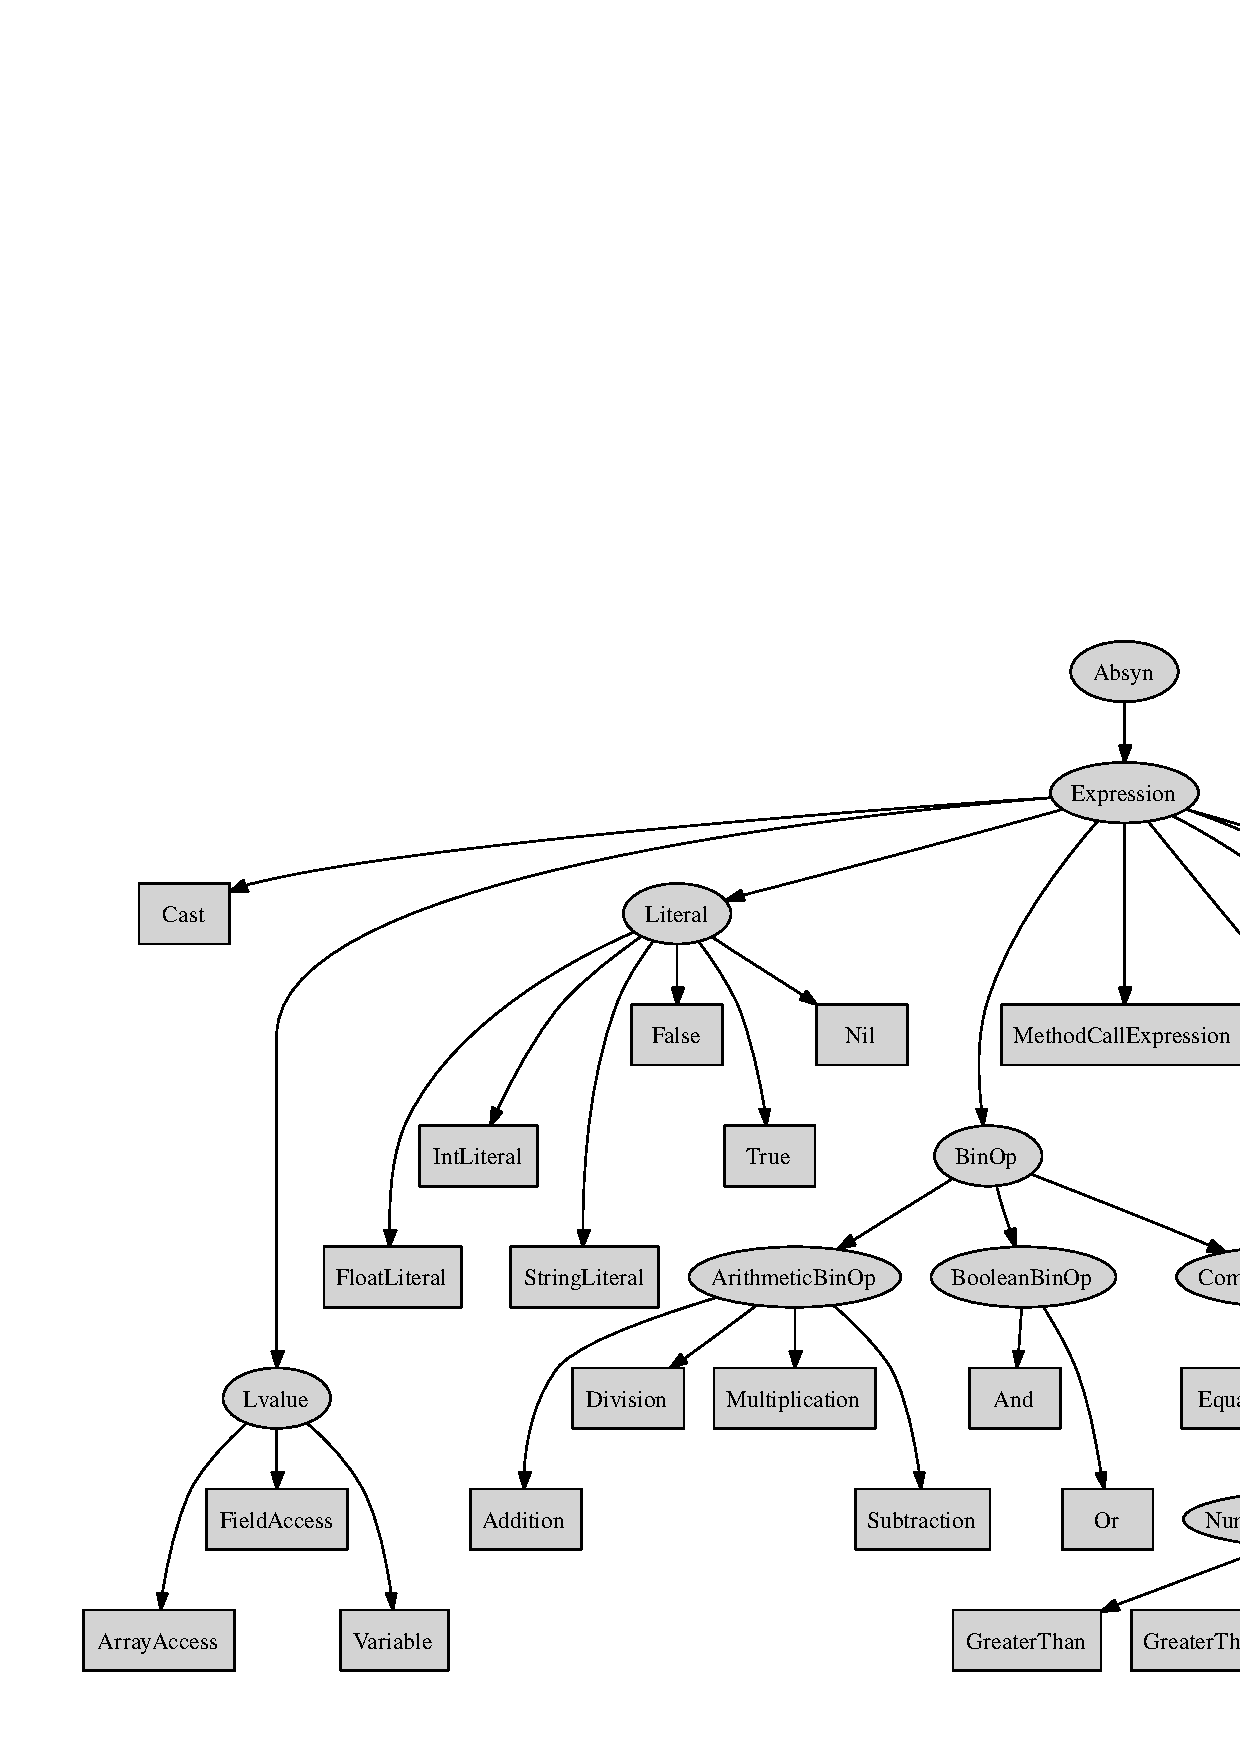
\epsfig{file = expressions_hierarchy.pdf, width = 15.5cm}
\end{center}
\caption{La struttura gerarchica delle classi di sintassi astratta per
         espressioni e leftvalue. Le classi astratte sono indicate con un
         ovale, quelle concrete con un rettangolo.}
  \label{fig:expressions_hierarchy}
\end{figure}
%
\begin{verbatim}
  lvalue ::=
     ID:id
     {: RESULT = new Variable(idleft,Symbol.mk(id)); :}
   | exp:receiver DOT:d ID:field
     {: RESULT = new FieldAccess(dleft,receiver,Symbol.mk(field)); :}
   | exp:array LBRACK:b exp:index RBRACK
     {: RESULT = new ArrayAccess(bleft,array,index); :} ;
\end{verbatim}

La Figura~\ref{fig:expressions_hierarchy} mostra la complessit\`a della
gerarchia delle classi di sintassi astratta per le
espressioni che sono operatori binari. Tali espressioni
sono in primo luogo divise
in \emph{aritmetiche} (\texttt{ArithmeticBinOp}),
\emph{booleane} (\texttt{BooleanBinOp}) e
\emph{di confronto} (\texttt{ComparisonBinOp}).
Queste ultime sono a loro volta divise in operazioni di confronto
che possono operare su qualsiasi tipo di valore, come
l'uguaglianza e la disuguaglianza, e in operazioni di confronto
che operano solo su numeri (interi o in virgola mobile),
incluse nella classe \texttt{NumericalComparisonBinOp}.
%
\subsection{Le classi di sintassi astratta per i comandi}
  \label{subsec:commands_abstract}
%
\begin{figure}[t]
\begin{center}
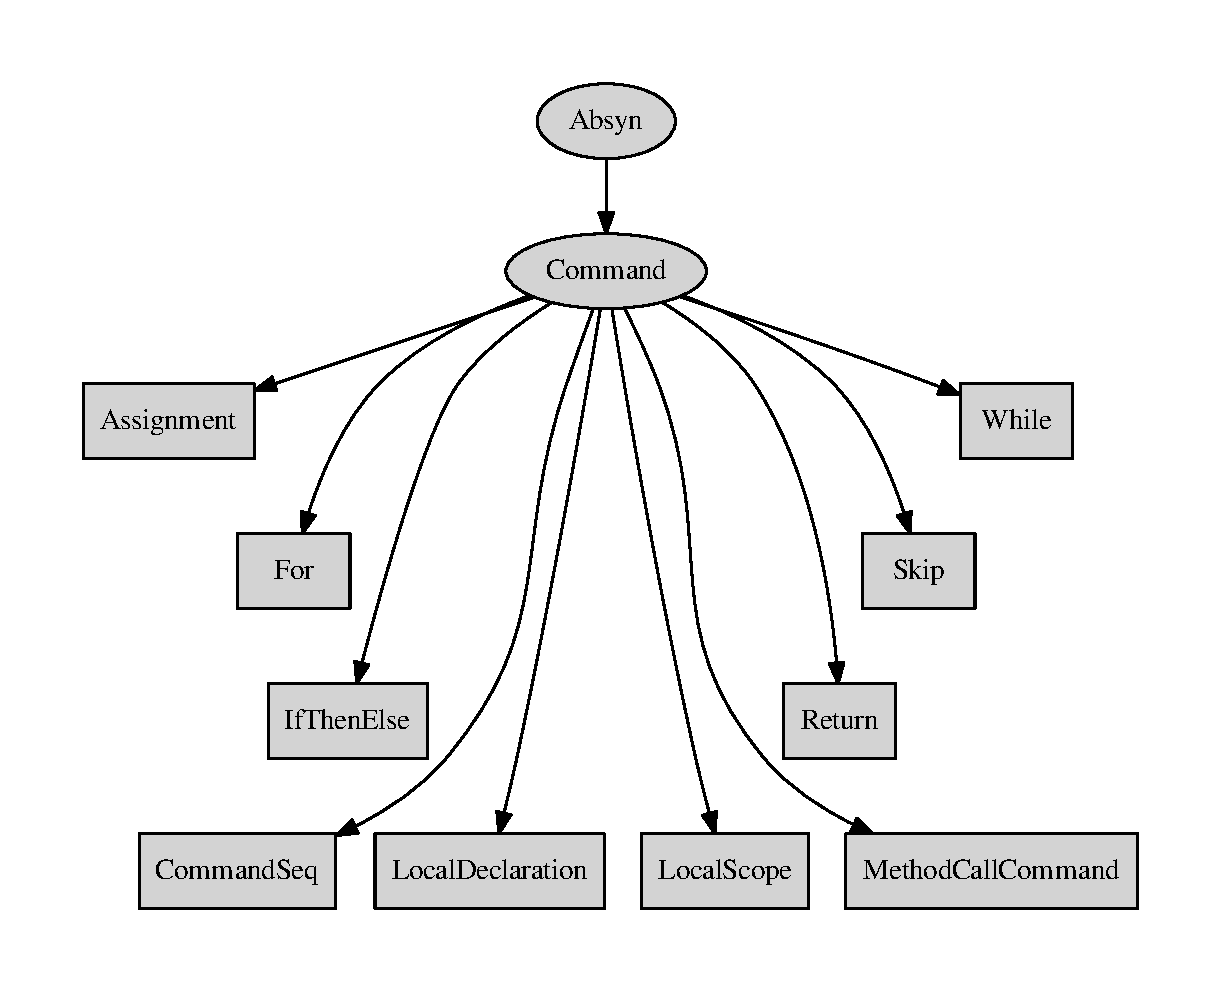
\epsfig{file = commands_hierarchy.pdf, width = 10cm}
\end{center}
\caption{La struttura gerarchica delle classi di sintassi astratta per
         i comandi. Le classi astratte sono indicate con un
         ovale, quelle concrete con un rettangolo.}
  \label{fig:commands_hierarchy}
\end{figure}
%
La Figura~\ref{fig:commands_hierarchy} mostra le classi di sintassi astratta
per i comandi. Si tratta di una gerarchia relativamente semplice.
La classe \texttt{LocalDeclaration} \`e
utilizzata per rappresentare la dichiarazione di una variabile.
La classe \texttt{Skip} \`e usata per rappresentare un comando vuoto,
come per esempio il corpo \verb!{}! del costruttore della classe in
Figura~\ref{fig:fibonacci}.
La classe \texttt{IfThenElse} \`e utilizzata per rappresentare sia il
condizionale semplice che quello composto, \cioe munito del ramo \texttt{else}.
Questo \`e evidente osservando le azioni semantiche per tale comando:
%
\begin{verbatim}
  command ::=
     IF:i LPAREN exp:condition RPAREN THEN command:then
      {: RESULT = new IfThenElse(ileft,condition,then); :}
   | IF:i LPAREN exp:condition RPAREN THEN command:then ELSE command:else
      {: RESULT = new IfThenElse(ileft,condition,then,else); :}
\end{verbatim}
%
Il costruttore a soli tre argomenti della classe
\texttt{absyn/IfThenElse.java} \`e definito in modo da chiamare
quello a quattro argomenti passando come quarto argomento un ramo
\texttt{else} vuoto, \cioe un'oggetto creato come
\texttt{new Skip(pos)}. In questo modo d'ora in poi possiamo sempre
assumere che i condizionali abbiano sempre un ramo \texttt{else}.

Le classi astratte per i comandi hanno un campo
\texttt{next} che lega in sequenza comandi contigui.
Il costruttore di \texttt{absyn/Command.java} annulla tale campo,
che deve essere settato in seguito quando si riconoscono due comandi
contigui. Questo \`e effettuato tramite il metodo \texttt{link()} della
classe \texttt{absyn/Command.java}, utilizzato nelle produzioni per gli
statements:
%
\begin{verbatim}
  statements ::=
     command:cmd
     {: RESULT = cmd; :}
   | command:cmd SEMICOLON statements:next
     {: cmd.link(next); RESULT = cmd; :} ;
\end{verbatim}

Anche per i comandi e gli statement
dobbiamo dichiarare il tipo del loro valore semantico, che \`e la
superclasse di tutte le classi di sintassi astratta per i comandi:
%
\begin{verbatim}
  non terminal Command statements;
  non terminal Command command;
\end{verbatim}
%
\subsection{Le classi di sintassi astratta per le classi Kitten}
  \label{subsec:classes_abstract}
%
\begin{figure}[t]
\begin{center}
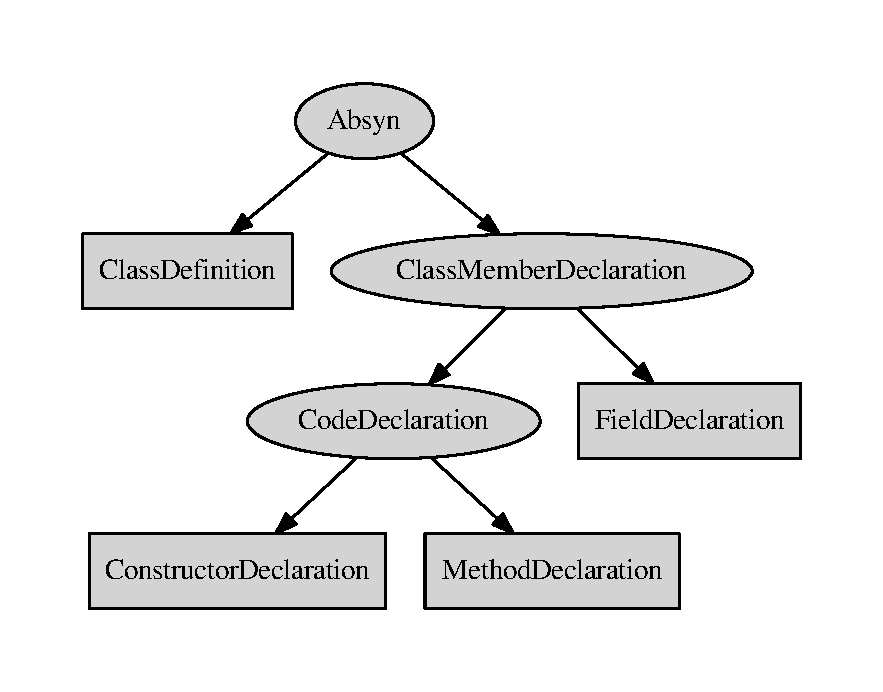
\epsfig{file = classes_hierarchy.pdf, width = 11cm}
\end{center}
\caption{La struttura gerarchica delle classi di sintassi astratta usate
         per rappresentare le classi Kitten.
         Le classi astratte sono indicate con un
         ovale, quelle concrete con un rettangolo.}
  \label{fig:classes_hierarchy}
\end{figure}
%
La Figura~\ref{fig:classes_hierarchy} mostra le classi di sintassi astratta
utilizzate per rappresentare la sintassi delle classi
Kitten. Una classe Kitten \`e rappresentata da un oggetto
di classe \texttt{ClassDefinition} al cui interno si trova una
lista di \texttt{ClassMemberDeclaration}. Ciascuna di tali dichiarazioni
dichiara un membro della classe, che pu\`o essere la dichiarazione di
un campo, di un costruttore o di un metodo.

Le produzioni che istanziano queste classi di sintassi astratta sono le
seguenti (si confronti con la Sezione~\ref{subsec:classes_specification}):
%
\begin{verbatim}
  class ::=
     CLASS:c ID:name LBRACE class_members:declarations RBRACE
      {: RESULT = new ClassDefinition
        (cleft,Symbol.mk(name),Symbol.OBJECT,declarations); :}
   | CLASS:c ID:name EXTENDS ID:superclass
       LBRACE class_members:declarations RBRACE
      {: RESULT = new ClassDefinition
        (cleft,Symbol.mk(name),Symbol.mk(superclass),declarations); :} ;

  class_members ::=
      {: RESULT = null; :}
   | FIELD:f type:t ID:name class_members:next
      {: RESULT = new FieldDeclaration(fleft,t,sym(name),next); :}
   | CONSTRUCTOR:c LPAREN formals:formals RPAREN command:body
       class_members:next
      {: RESULT = new ConstructorDeclaration(cleft,formals,body,next); :}
   | METHOD:m typeplus:returnType ID:name LPAREN formals:formals RPAREN
       command:body class_members:next
      {: RESULT = new MethodDeclaration
        (mleft,returnType,sym(name),formals,body,next); :} ;
\end{verbatim}
%
Si noti che nel caso in cui la superclasse di una classe Kitten non \`e
specificata si assume che essa sia \texttt{Object}, in modo che possiamo
sempre assumere che una classe Kitten abbia specificata la sua superclasse.

I tipi dei non terminali sono dichiarati come:
%
\begin{verbatim}
  non terminal ClassDefinition         class;
  non terminal ClassMemberDeclaration  class_members;
\end{verbatim}
%
\begin{figure}
\begin{center}
{\scriptsize
\begin{tabular}{l}
\textit{Absyn()} \\
\texttt{Addition(Expression left, Expression right)} \\
\texttt{And(Expression left, Expression right)} \\
\textit{ArithmeticBinOp(Expression left, Expression right)} \\
\texttt{ArrayAccess(Expression array, Expression index)} \\
\texttt{ArrayTypeExpression(TypeExpression elementsType)} \\
\texttt{Assignment(Lvalue lvalue, Expression rvalue)} \\
\textit{BinOp(Expression left, Expression right)} \\
\textit{BooleanBinOp(Expression left, Expression right)} \\
\texttt{BooleanTypeExpression()} \\
\texttt{Cast(TypeExpression type, Expression expression)} \\
\texttt{ClassDefinition(Symbol name, Symbol superclassName, ClassMemberDeclaration declaration)} \\
\textit{ClassMemberDeclaration(ClassMemberDeclaration next)} \\
\texttt{ClassTypeExpression(Symbol name)} \\
\textit{CodeDeclaration(FormalParameters formals, Command body, ClassMemberDeclaration next)} \\
\textit{Command()} \\
\textit{ComparisonBinOp(Expression left, Expression right)} \\
\texttt{ConstructorDeclaration(FormalParameters formals, Command body, ClassMemberDeclaration next)} \\
\texttt{Division(Expression left, Expression right)} \\
\texttt{Equal(Expression left, Expression right)} \\
\textit{Expression()} \\
\texttt{ExpressionSeq(Expression head, ExpressionSeq tail)} \\
\texttt{False()} \\
\texttt{FieldAccess(Expression receiver, Symbol name)} \\
\texttt{FieldDeclaration(TypeExpression type, Symbol name, ClassMemberDeclaration next)} \\
\texttt{FloatLiteral(float value)} \\
\texttt{FloatTypeExpression()} \\
\texttt{For(Command initialisation, Expression condition, Command update, Command body)} \\
\texttt{FormalParameters(TypeExpression type, Symbol name, FormalParameters next)} \\
\texttt{GreaterThan(Expression left, Expression right)} \\
\texttt{GreaterThanOrEqual(Expression left, Expression right)} \\
\texttt{IfThenElse(Expression condition, Command then, Command else)} \\
\texttt{IntLiteral(float value)} \\
\texttt{IntTypeExpression()} \\
\texttt{LessThan(Expression left, Expression right)} \\
\texttt{LessThanOrEqual(Expression left, Expression right)} \\
\textit{Literal()} \\
\texttt{LocalDeclaration(TypeExpression type, Symbol name, Expression initialiser)} \\
\texttt{LocalScope(Command body)} \\
\textit{Lvalue()} \\
\texttt{MethodCallCommand(Expression receiver, Symbol name, ExpressionSeq actuals)} \\
\texttt{MethodCallExpression(Expression receiver, Symbol name, ExpressionSeq actuals)} \\
\texttt{MethodDeclaration(TypeExpression returnType, Symbol name, FormalParameters formals,}\\
\hspace*{21ex}\texttt{Command body, ClassMemberDeclaration next)} \\
\texttt{Minus(Expression expression)} \\
\texttt{Multiplication(Expression left, Expression right)} \\
\texttt{NewArray(TypeExpression elementsType, Expression size)} \\
\texttt{NewObject(Symbol className, ExpressionSeq actuals)} \\
\texttt{Nil()} \\
\texttt{Not(Expression expression)} \\
\texttt{NotEqual(Expression left, Expression right)} \\
\textit{NumericalComparisonBinOp(Expression left, Expression right)} \\
\texttt{Or(Expression left, Expression right)} \\
\texttt{Return(Expression returned)} \\
\texttt{Skip()} \\
\texttt{StringLiteral(String value)} \\
\texttt{Subtraction(Expression left, Expression right)} \\
\texttt{True()} \\
\textit{TypeExpression()} \\
\texttt{Variable(Symbol name)} \\
\texttt{VoidTypeExpression()} \\
\texttt{While(Expression condition, Command body)}
\end{tabular}
}
\end{center}
\caption{Una visione d'insieme delle classi di sintassi astratta del linguaggio Kitten. Le classi in \emph{italico} sono classi astratte, nel senso di Java.}
  \label{fig:abstract_classes}
\end{figure}
%
\subsection{Un riassunto delle classi di sintassi astratta di Kitten}
  \label{subsec:abstract_classes}
%
In Figura~\ref{fig:abstract_classes} riportiamo un elenco riassuntivo delle
classi di sintassi astratta di Kitten. Per ogni classe riportiamo il
costruttore, che d\`a anche informazione sul contenuto degli oggetti di tale
classe. Per esempio, la notazione:
%
\begin{verbatim}
  Addition(Expression left, Expression right)
\end{verbatim}
%
indica che la classe di sintassi astratta \texttt{absyn/Addition.java}
ha due campi, \texttt{left} e \texttt{right}, di tipo
\texttt{Expression}. Il suo costruttore ha in effetti \emph{tre} parametri:
oltre ai due riportati, \`e sottointeso anche un primo parametro \texttt{pos}
di tipo \texttt{int} che indica la posizione del file sorgente in cui segnalare
un errore in fase di analisi semantica se qualcosa non torna su questa parte
di sintassi. Per semplicit\`a, in Figura~\ref{fig:abstract_classes}
non abbiamo riportato tale ulteriore parametro.

La Figura~\ref{fig:abstract_classes} \`e compatibile
con l'albero di sintassi astratta in Figura~\ref{fig:led_albero}.
Per esempio, il nodo etichettato con
\texttt{Not} in Figura~\ref{fig:led_albero}
rappresenta un oggetto di classe \texttt{Not} il cui
costruttore, in Figura~\ref{fig:abstract_classes}, ha intestazione
\texttt{Not(Expression expression)}. L'espressione negata \`e infatti
legata in Figura~\ref{fig:led_albero} tramite un arco etichettato con
\texttt{expression} a un nodo di tipo \texttt{FieldAccess}, che
\`e sottoclasse di \texttt{Expression}
(Figura~\ref{fig:expressions_hierarchy}).
Tale nodo di tipo \texttt{FieldAccess} \`e poi legato, in
Figura~\ref{fig:led_albero}, tramite due archi etichettati con
\texttt{receiver} e \texttt{name}, a due nodi di tipo, rispettivamente,
\texttt{Variable} e \texttt{Symbol} (rettangolare). Questo
rispetta il costruttore di \texttt{FieldAccess} in
Figura~\ref{fig:abstract_classes}, che \`e
\texttt{FieldAccess(Expression receiver, Symbol name)}.
Si noti che \texttt{Variable} \`e una sottoclasse di \texttt{Expression}
(Figura~\ref{fig:expressions_hierarchy}).

Ricordiamo che ulteriori informazioni sulle classi di sintassi astratta sono
disponibili con la distribuzione di Kitten, sotto forma di documentazione
JavaDoc.

\chapter{Discesa Ricorsiva sulla Sintassi Astratta}
  \label{chap:recursive_descent}
%
\begin{center}
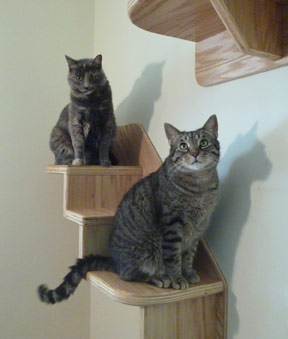
\includegraphics[width=6cm]{paw.jpg}
\end{center}
%
In questo capitolo discutiamo l'implentazione di algoritmi che
scendono ricorsivamente sull'albero di sintassi astratta che l'analizzatore
sintattico ha generato a partire da un file sorgente. Tali algoritmi
hanno le funzioni pi\`u svariate, da una semplice raccolta di dati statistici
sul codice alla verifica dell'uso corretto degli identificatori,
dalla determinazione del \emph{codice morto}, \cioe di porzioni di codice
che sicuramente non vengono raggiunte dal flusso di controllo e possono
quindi essere eliminate,
alla rappresentazione grafica della sintassi astratta, fino
al type-checking del codice (a cui dedicheremo,
per la sua complessit\`a, l'intero Capitolo~\ref{chap:semantical})
o addirittura alla generazione del codice intermedio,
descritta nel Capitolo~\ref{chap:translate}.
L'implementazione di questi algoritmi tramite discesa ricorsiva
sulla sintassi astratta, piuttosto
che tramite azioni semantiche (Capitolo~\ref{chap:syntactical}),
permette di sfruttare la gerarchia delle classi di sintassi astratta per
Kitten descritta nel Capitolo~\ref{chap:syntactical}, definendo l'algoritmo
ricorsivo tramite un metodo virtuale ricorsivo delle classi di sintassi
astratta.

Si consideri per esempio la grammatica in Figura~\ref{fig:grammar_lists}.
Supponiamo di voler contare
il numero di \texttt{a} e il numero di \texttt{b} di ciascun file sorgente
che rispetta le regole espresse dalla grammatica. Abbiamo gi\`a risolto questo
problema in Figura~\ref{fig:grammar_lists_decoration} tramite azioni
semantiche. Ma possiamo fare la stessa cosa generando la sintassi astratta
tramite le regole in Figura~\ref{fig:grammar_lists_abstract_syntax} e
aggiungendo alle classi di sintassi astratta un metodo
\texttt{count()} che conta il numero di \texttt{a} o di \texttt{b}
contenute nella sintassi concreta rappresentata dall'albero di sintassi
astratta. Il codice \`e mostrato nella Figura~\ref{fig:grammar_lists_count}.
Le classi \texttt{AbstractA}, \texttt{EmptyA} e \texttt{OneA} sono
simili a quelle mostrate nella figura per \texttt{B}.
La classe \texttt{Pair} \`e la
stessa usata nella Sezione~\ref{sec:abstract_syntax} (una coppia di interi).
%
\begin{figure}[t]
\begin{verbatim}
     public abstract class AbstractB {
       public abstract int count();
     }

     public class EmptyB extends AbstractB {
       public int count() { return 0; }
     }

     public class OneB extends AbstractB {
       private final AbstractB l;
       public OneB(AbstractB l) { this.l = l; }
       public int count() { return 1 + l.count(); }
     }

     public class AB {
       private final AbstractA a;
       private final AbstractB b;
       public AB(AbstractA a, AbstractB b) { this.a = a; this.b = b; }
       public Pair count() {
         return new Pair(a.count(), b.count());
       }
     }
\end{verbatim}
\caption{Un metodo ricorsivo che conta il numero di \texttt{a} e di \texttt{b}
         nella sintassi astratta generata come in
         Figura~\ref{fig:grammar_lists_decoration}.}
  \label{fig:grammar_lists_count}
\end{figure}

Va subito osservato che in Figura~\ref{fig:grammar_lists_count} sono
definiti \emph{due} metodi \texttt{count()}. Il primo \`e quello
ricorsivo delle classi \texttt{EmptyB} e \texttt{OneB}; il secondo \`e quello
\emph{non ricorsivo} della classe \texttt{AB}. Esiste anche un metodo
\texttt{count()} ricorsivo dentro \texttt{EmptyA} e \texttt{OneA} che non
\`e mostrato in figura in quanto \`e simmetrico a quello in
\texttt{EmptyB} e \texttt{OneB}.
Il metodo \texttt{count()} di \texttt{EmptyB} e \texttt{OneB} \`e
\emph{a discesa ricorsiva sulla sintassi astratta} poich\'e la sua
chiamata scende ricorsivamente sui componenti della sintassi astratta fino
ad arrivare alle foglie, per le quali \`e definito un valore costante.
Si faccia attenzione al fatto che
il metodo virtuale \texttt{count()} \`e dichiarato
\texttt{abstract} nella superclasse astratta \texttt{AbstractB} e quindi
\emph{deve} essere implementato in ognuna delle sue sottoclassi.

Cosa abbiamo guadagnato rispetto all'uso di azioni semantiche come
in Figura~\ref{fig:grammar_lists_decoration}? In primo luogo abbiamo lasciato
l'analizzatore sintattico alla sua occupazione pi\`u specifica, \cioe
all'analisi sintattica, piuttosto che usarlo per funzioni a lui \emph{improprie}
tramite azioni semantiche, rispettando quindi il principio della separation
of concerns. In secondo luogo abbiamo \emph{concentrato}
delle funzioni della sintassi astratta nelle classi di sintassi astratta
stesse, sotto forma di codice Java ricorsivo, che pu\`o essere complesso
quanto vogliamo. In terzo luogo possiamo utilizzare la gerarchizzazione delle
classi di sintassi astratta (come quella discussa per Kitten nella
Sezione~\ref{sec:abstract_syntax_classes}) per definire i metodi virtuali
solo su alcune superclassi, lasciandoli ereditare a tutte le loro sottoclassi,
nei casi in cui essi non differissero da una sottoclasse all'altra.
Questo non \`e possibile tramite azioni semantiche che, anche quando sono
identiche per \piu produzioni della grammatica,
devono essere comunque duplicate per ognuna di esse.
Quest'ultimo aspetto sar\`a chiaro adesso considerando un esempio di
discesa ricorsiva sulla sintassi astratta di Kitten.
%
\section{Determinazione delle variabili che occorrono in un'espressione o comando}
  \label{sec:free_variables}
%
Espressioni e comandi Kitten possono contenere variabili.
Per esempio, le variabili che \emph{occorrono} (sono contenute)
nell'espressione Kitten \texttt{x + 3 * y} sono \texttt{x} e \texttt{y}.
Le variabili che occorrono nel comando Kitten
\texttt{x := 12 + a} sono \texttt{x} e \texttt{a}.
Ci proponiamo adesso di definire formalmente e poi di calcolare l'insieme delle
variabili che occorrono in un'espressione e poi l'insieme delle variabili che
occorrono in un comando.

Cominciamo con le espressioni (Figura~\ref{fig:expressions_hierarchy}).
Definiamo una funzione
\[
  \vars{\_}:\mathtt{Expression}\mapsto\wp(\mathtt{String})
\]
che mappa ciascuna espressione nell'insieme dei nomi delle variabili
che occorrono nell'espressioni. Alcuni casi della
definizione di questa funzione sono particolarmente semplici. Per esempio,
una variabile occorre in se stessa:
\begin{equation}\label{eq:vars_variable}
  \vars{\mathtt{Variable(name)}}=\{\mathtt{name}\}
\end{equation}
mentre i letterali non contengono variabili:
\begin{equation}\label{eq:vars_literal}
  \vars{\mathtt{Literal()}}=\emptyset~.
\end{equation}
Si noti che quest'ultima equazione definisce l'insieme delle variabili che
occorrono in ogni sottoclasse di \texttt{Literal} in
Figura~\ref{fig:expressions_hierarchy}, senza bisogno di ripetere l'equazione
per ogni sottoclasse.

Un po' \piu complesso \`e il caso del meno unario e della negazione logica che,
che contenendo ricorsivamente un'altra espressione, danno origine a una
definizione ricorsiva per $\vars{}$ (ma ben fondata perch\'e andiamo verso
strutture sintattiche sempre \piu piccole):
\[
  \vars{\mathtt{Minus(expression)}}=\vars{\mathtt{Not(expression)}}
    =\vars{\mathtt{expression}}~.
\]
Un cast e la creazione di un array contengono sia un tipo che un'espressione.
Il tipo non contribuisce alle variabili, ma solo l'espressione:
%
\begin{align*}
  \vars{\mathtt{Cast(type,expression)}}&=\vars{\mathtt{expression}}\\
  \vars{\mathtt{NewArray(elementsType,size)}}&=\vars{\mathtt{size}}~.
\end{align*}
%
Similmente per l'accesso a un campo, in cui l'identificatore fa riferimento
a un campo e non a una variabile e quindi non \`e di nostro interesse in questo
contesto:
%
\begin{equation}\label{eq:vars_fieldaccess}
  \vars{\mathtt{FieldAccess(receiver,name)}}=\vars{\mathtt{receiver}}~.
\end{equation}
%
La definizione per \emph{tutti} gli operatori binari pu\`o venire data come:
\begin{equation}\label{eq:vars_binop}
  \vars{\mathtt{BinOp(left,right)}}=\vars{\mathtt{left}}\cup
    \vars{\mathtt{right}}
\end{equation}
%
e similmente quella per l'accesso a un elemento di un array (sia l'array che
l'indice dell'elemento sono espressioni):
\[
  \vars{\mathtt{ArrayAccess(array,index)}}=\vars{\mathtt{array}}\cup
    \vars{\mathtt{index}}~.
\]
%
Rimangono le chiamate di metodo e la creazione di un oggetto, che contengono
una lista di espressioni (parametri). Definiamo
l'insieme delle variabili che occorrono in una lista di espressioni come
l'unione delle variabili che occorrono in ciascuna espressione:
%
\begin{align*}
  \vars{\mathtt{MethodCallExpression(receiver,name,actuals)}}
    &=\vars{\mathtt{receiver}}\\
  &\quad\cup\ \vars{\mathtt{actuals}}\\
  \vars{\mathtt{NewObject(className,actuals)}}&=\vars{\mathtt{actuals}}
\end{align*}
%
dove $\vars{\_}:\mathtt{ExpressionSeq}\mapsto\wp(\mathtt{String})$ \`e
definito come
%
\begin{align*}
  \vars{\mathtt{null}}&=\emptyset\\
  \vars{\mathtt{ExpressionSeq(head,tail)}}&=\vars{\mathtt{head}}\cup
    \vars{\mathtt{tail}}~.
\end{align*}

Consideriamo adesso i comandi (Figura~\ref{fig:commands_hierarchy}).
Estendiamo la funzione $\vars{\_}$ in modo da potere essere applicata anche
ai comandi:
\[
  \vars{\_}:\mathtt{Command}\mapsto\wp(\mathtt{String})~.
\]
%
L'idea \`e semplicissima: le variabili che occorrono in un comando sono
quelle che occorrono in uno qualsiasi dei componenti del comando
(espressioni o sotto-comandi). Inoltre una sequenza di comandi separati
da punto e virgola contiene l'unione delle variabili contenute in ciascun
comando:
%
\begin{align}
  \notag
  \vars{\mathtt{Assignment(lvalue,rvalue)}}
    &=\vars{\mathtt{lvalue}}\cup\vars{\mathtt{rvalue}}\\\notag
  \vars{\mathtt{For(initialisation,condition,update,body)}}
    &=\vars{\mathtt{initialisation}}\\\notag
      &\quad\cup\ \vars{\mathtt{condition}}\\\notag
      &\quad\cup\ \vars{\mathtt{update}}\\\notag
      &\quad\cup\ \vars{\mathtt{body}}\\
  \label{eq:vars_ifthenelse}
  \vars{\mathtt{IfThenElse(condition,then,else)}}
    &=\vars{\mathtt{condition}}\\\notag
      &\quad\cup\ \vars{\mathtt{then}}\cup
      \vars{\mathtt{else}}\\\notag
  \vars{\mathtt{LocalDeclaration(type,name,initialiser)}}
    &=\{\mathtt{name}\}\cup\vars{\mathtt{initialiser}}\\\notag
  \vars{\mathtt{LocalScope(body)}}&=\vars{\mathtt{body}}\\\notag
  \vars{\mathtt{MethodCallCommand(receiver,name,actuals)}}&=
    \vars{\mathtt{receiver}}\\\notag
  &\quad\cup\ \vars{\mathtt{actuals}}\\\notag
  \vars{\mathtt{Return(returned)}}&=\vars{\mathtt{returned}}\\\notag
  \vars{\mathtt{Skip()}}&=\emptyset\\\notag
  \vars{\mathtt{While(condition,body)}}&=\vars{\mathtt{condition}}\cup
    \vars{\mathtt{body}}\\
  \label{eq:vars_sequence}
  \vars{\mathtt{CommandSeq(first,second)}}&=\vars{\mathtt{first}}\cup\vars{\mathtt{second}}~.
\end{align}

Consideriamo adesso l'implementazione in Java della funzione
$\vars{}$ che abbiamo appena finito di definire. L'idea \`e di aggiungere
un metodo \texttt{vars()} alle classi di sintassi astratta per
espressioni e comandi. Cominciamo dichiarandoli \texttt{abstract}
all'interno delle superclassi astratte di tutte le espressioni e di
tutti i comandi:
%
\begin{verbatim}
  public class Expression extends Absyn {
    ....
    public abstract Set<String> vars();
  }

  public class Command extends Absyn {
    ...
    public abstract Set<String> vars();
  }
\end{verbatim}
%
A questo punto abbiamo l'obbligo di istanziare tale metodo in tutte
le sottoclassi di \texttt{Expression} (Figura~\ref{fig:expressions_hierarchy})
e in tutte le sottoclassi di \texttt{Command}
(Figura~\ref{fig:commands_hierarchy}). Il compito sembra gravoso ma \`e
in realt\`a semplificato dalla gerachia delle classi. Per esempio,
l'Equazione~\eqref{eq:vars_variable} viene implementata modificando la
classe \texttt{absyn/Variable.java}:
%
\begin{verbatim}
  public class Variable extends Lvalue {
    ...
    public Set<String> vars() {
      Set<String> result = new HashSet<String>();
      result.add(name);
      return result;
    }
  }
\end{verbatim}
%
e l'Equazione~\eqref{eq:vars_literal} viene implementata
\emph{per tutti i letterali} modificando soltanto
la loro superclasse \texttt{absyn/Literal.java}:
%
\begin{verbatim}
  public class Literal extends Expression {
    ...
    public final Set<String> vars() {
      return new HashSet<String>();  // insieme vuoto
    }
  }
\end{verbatim}
%
Si noti che il metodo \texttt{vars()} di \texttt{absyn/Literal.java} \`e
lasciato ereditare a tutte le sue sottoclassi, che quindi non ne ricevono
una definizione esplicita.

Definizioni ricorsive diventano implementazioni ricorsive del metodo
\texttt{vars()}. Per esempio, l'Equazione~\eqref{eq:vars_fieldaccess}
\`e implementata modificando coma segue
la classe \texttt{absyn/FieldAccess.java}:
%
\begin{verbatim}
  public class FieldAccess extends Lvalue {
    ...
    public Set<String> vars() {
      return receiver.vars();
    }
  }
\end{verbatim}

Il metodo \texttt{vars()}
\emph{per tutti gli operatori binari} \`e definito modificando, in accordo
con l'Equazione~\eqref{eq:vars_binop}, la classe \texttt{absyn/BinOp.java}:
%
\begin{verbatim}
  public class BinOp extends Expression {
    ...
    public final Set<String> vars() {
      Set<String> result = new HashSet<String>();
      result.addAll(left.vars());
      result.addAll(right.vars());
      return result;
    }
  }
\end{verbatim}
%
\javatip{Ci si abitui a definire i metodi a discesa ricorsiva come
nell'esempio precedente, in cui \cioe il risultato delle chiamate ricorsive
non \`e modificato per costruire il risultato complessivo. Questo
approccio, che chiamiamo \emph{funzionale}, \`e preferibile a un approccio
\emph{distruttivo} del tipo
\texttt{Set<String> result = left.vars(); result.addAll(right.vars());}
in cui l'insieme proveniente dalla sotto-espressione \texttt{left}
\`e modificato aggiungendovi i simboli provenienti dalla sotto-espressione
\texttt{right}. Il motivo per cui preferiamo un approccio funzionale
\`e che quest'ultimo lascia immutati
i risultati intermedi delle chiamate ricorsive. Questi risultati potrebbero
essere salvati e poi riutilizzati in futuro. In alcuni casi un approccio
distruttivo pu\`o introdurre veri e propri errori di programmazione a causa
di una complessa condivisione di strutture dati che il programmatore non
riesce a dominare.}

Consideriamo adesso i comandi. Il metodo \texttt{vars()} per il comando
condizionale va scritto modificando, in accordo con
l'Equazione~\eqref{eq:vars_ifthenelse}, la classe
\texttt{absyn/IfThenElse.java}:
%
\begin{verbatim}
  public class IfThenElse extends Command {
    ...
    public Set<String> vars() {
      Set<String> result = new HashSet<String>();
      result.addAll(condition.vars());
      result.addAll(then.vars());
      result.addAll(else.vars());
      return result;
    }
  }
\end{verbatim}
%
Si osservi che, delle tre chiamate a \texttt{vars()}, la prima avviene
sulle espressioni mentre le due successive sui comandi.

Il metodo \texttt{vars()} per la sequenza di comandi va scritto modificando
la classe \texttt{absyn/CommandSeq.java}, in accordo con l'Equazione~\eqref{eq:vars_sequence}:
%
\begin{verbatim}
  public class CommandSeq extends Command {
    ...
    public Set<String> vars() {
      Set<String> result = new HashSet<String>();
      result.addAll(left.vars());
      result.addAll(right.vars());
      return result;
    }
  }
\end{verbatim}
%
\section{Determinazione delle variabili dichiarate ma non usate}
  \label{sec:no_use}
%
Kitten ammette di dichiarare variabili che poi non vengono usate all'interno
del loro scope di visibilit\`a. \`E comunque ovvio che la dichiarazione di
una variabili non usata \`e inutile e pu\`o essere eliminata dal programma
senza cambiare la semantica di quest'ultimo,
purch\'e l'inizializzatore della variabile non
contenga side-effect e la sua valutazione termini sempre.
Comunque sia, la dichiarazione
di una variabile non usata \`e spesso considerata erronea o sospetta
(\emph{warning}) in molti altri linguaggi di programmazione.

Supponiamo di volere aggiungere a Kitten la possibilit\`a di controllare
che il corpo di metodi e costruttori non dichiari mai variabili non utilizzate.
Facciamo l'ipotesi semplificativa che ogni dichiarazione in un metodo o
costruttore introduca una variabile diversa, ovvero che non ci siano
\emph{sinonimi}. Questa ipotesi pu\`o essere rimossa ridenominando
opportunamente le variabili del programma.
Dal momento che il corpo di un metodo o costruttore \`e un comando $c$
(Sezione~\ref{subsec:classes_specification}), possiamo determinare l'insieme
delle variabili dichiarate ma non usate in $c$ come la sottrazione dell'insieme
delle variabili usate in $c$ da quello delle variabili dichiarate in $c$:
\[
  \declared{c}\setminus\used{c}~.
\]
Si noti che consideriamo solo le variabili dichiarate in $c$ e non
i parametri del metodo o costruttore e neppure il parametro implicito
\texttt{this}.
Questo implica che accettiamo l'idea che i parametri,
incluso il parametro implicito \texttt{this}, possano non venire usati
all'interno del metodo o costruttore, senza che questo comporti la segnalazione
di un warning al programmatore\footnote{Non utilizzare i parametri \`e
estremamente usuale in un contesto di programmazione a oggetti in cui i metodi
di una classe sono
spesso ottenuti per specializzazione da quelli della superclasse. Questa
ipotesi potrebbe quindi essere migliorata per i soli metodi privati di una
classe, ma Kitten non ammette metodi privati.}.

Sappiamo gi\`a calcolare l'insieme delle variabili che \emph{occorrono}
in un comando (Sezione~\ref{sec:free_variables}). L'insieme delle variabili
\emph{usate} in un comando coincide con l'insieme calcolato dalla funzione
$\vars{}$ se non fosse che la dichiarazione di una variabile non deve essere
considerata come un uso della stessa. Conseguentemente la definizione
di $\used{}$ \`e identica a quella di $\vars{}$ data nella
Sezione~\ref{sec:free_variables} con l'unica differenza che
\[
  \used{\mathtt{LocalDeclaration(type,name,initialiser)}}
    =\used{\mathtt{initialiser}}~.
\]

Invece dobbiamo ancora definire l'insieme delle variabili
\emph{dichiarate} in un comando. Lo facciamo dicendo che normalmente un
comando non dichiara alcuna variabile:
%
$
  \declared{\mathit{c}}=\emptyset
$,
%
ma la dichiarazione di variabile fa ovviamente eccezione alla regola
generale:
%
\[
  \declared{\mathtt{LocalDeclaration(type,name,initialiser)}}
    =\{\mathtt{name}\}~.
\]
%
Infine, l'insieme delle variabili dichiarate in una sequenza di comandi
separati da punto e virgola \`e l'unione degli insiemi delle variabili
dichiarate in ciascun comando della sequenza:
%
\[
  \declared{\mathtt{CommandSeq(first,second)}}=\declared{\mathtt{first}}
    \cup\declared{\mathtt{second}}~.
\]

L'implementazione in Java della funzione $\used{}$ \`e quasi identica
all'implementazione della funzione $\vars{}$, vista nella
Sezione~\ref{sec:free_variables}. L'unica differenza \`e per la dichiarazione
di variabile. L'implementazione della funzione $\declared{}$ invece
\`e interessante poich\'e permette di sfruttare la gerarchia delle
classi in Figura~\ref{fig:commands_hierarchy}. Definiamo infatti un
comportamento di default per il metodo \texttt{declared()} che aggiungiamo
ai comandi:
%
\begin{verbatim}
  public class Command extends Absyn {
    ...
    public Set<String> declared() {
      return new HashSet<String>();    // un insieme vuoto
    }
  }
\end{verbatim}
%
Quindi definiamo l'unica eccezione in \texttt{absyn/LocalDeclaration.java}
ridefinendovi il metodo \texttt{declared()}:
%
\begin{verbatim}
  public class LocalDeclaration extends Command {
    ...
    public Set<String> declared() {
      Set<String> result = new HashSet<String>();
      result.add(name);
      return result;
    }
  }
\end{verbatim}
%
\greycomment{La tecnica descritta per determinare l'insieme delle variabili
dichiarate ma non usate \`e abbastanza rudimentale. Abbiamo gi\`a detto che
\`e necessario supporre che non ci siano variabili con lo stesso
nome dichiarate all'interno dello stesso metodo o costruttore. Inoltre la
tecnica restituisce
solo i nomi delle variabili che sono state dichiarate ma non usate.
Conseguemente possiamo dare un errore solo alla fine del metodo piuttosto
che nel punto esatto in cui la variabile \`e stata dichiarata (si potrebbe
ridiscendere sulla sintassi astratta per segnalare l'errore al posto
giusto\ldots). Infine osserviamo che questo metodo non capisce se una
variabile \`e usata solo all'interno di una parte di codice che non verr\`a
mai eseguita, nel qual caso essa non \`e \emph{realmente} usata.
E non si potr\`a mai risolvere del tutto questo problema
poich\'e l'eseguibilit\`a di porzioni di codice \`e una propriet\`a
indecibile.
Come per tutte le propriet\`a \emph{interessanti} di programmi, dovremo
accontentarci di approssimazioni per le informazioni che cerchiamo, purch\'e
esse siano approssimazioni \emph{corrette}. Per esempio, in questa sezione
la correttezza significa che se una variabile sta in
$\declared{c}\setminus\vars{c}$ allora sicuramente essa \`e stata dichiarata
ma non usata in $c$. Non abbiamo nessuna garanzia del contrario:
basta considerare
il comando \texttt{int y := 4; if (x = x) then \{\} else x := y} in cui
\texttt{y} \`e solo apparentemente usata, poich\'e il ramo \texttt{else}
del condizionale non verr\`a mai eseguito. Ovviamente questo esempio
pu\`o essere complicato a piacere, essendo il problema indecibile.}
%
\section{Determinazione del codice morto}\label{sec:dead_code}
%
Un comando \`e detto \emph{codice morto} in un programma se esso non
verr\`a mai eseguito, indipendentemente dall'input fornito al programma.
Conseguentemente, tale comando \`e \emph{inutile} e potrebbe essere eliminato.
Determinare se un comando \`e codice morto \`e un problema indecidibile.
Ci accontenteremo quindi di una approssimazione \emph{corretta} dell'insieme
del codice morto, nel senso che
se riusciremo a determinare che un comando \`e codice morto allora esso
lo \`e realmente, ma il viceversa in genere non sar\`a vero: ci sar\`a
del codice morto che sfuggir\`a alla nostra tecnica di ricerca.

Un esempio di codice morto \`e l'ultimo comando del seguente metodo:
%
\begin{verbatim}
  method int fib(int i) {
    if (i < 2) then return 1
    else return this.fib(i - 1) + this.fib(i - 2);

    "ciao".output()
  }
\end{verbatim}
%
Il motivo \`e che la linea \verb!"ciao".output()! non pu\`o mai essere
raggiunta. Evitare la compilazione
di programmi che contengono codice morto pu\`o sembrare eccessivamente
restrittivo, ma \`e invece spesso importante poich\'e costringe il
programmatore a ragionare sulla struttura di controllo del codice.
Molto spesso, infatti, la presenza di codice morto \`e un sintomo di
un bug in un programma.
%Pu\`o sembrare strano che il programmatore scriva comandi che non vengono
%mai eseguiti, ma questa situazione \`e in realt\`a frequente quando si
%utilizzano librerie esterne all'applicazione che si sta sviluppando:
%larghe porzioni della libreria non vengono mai usate o vengono
%usate con parametri \cosi specifici da non utilizzarne completamente il codice.
%Purtroppo queste situazioni sono tipicamente quelle pi\`u difficili da
%scoprire. Ci limiteremo quindi essenzialmente a quelle pi\`u facili da
%individuare, che sono spesso la conseguenza di errori di programmazione come
%istruzioni \texttt{return} dimenticate. Per esempio, vogliamo segnalare che
%nel comando
%
%\begin{verbatim}
%  x := x + 2; return; y := x * 3
%\end{verbatim}
%
%il sotto-comando \texttt{y := x * 3} \`e codice morto.
Si noti che, se ci fosse un ulteriore comando nel corpo del metodo precedente,
subito dopo il comando \verb!"ciao".output()!, allora preferiremmo
non segnalare che anche esso \`e codice morto, bench\'e effettivamente lo sia,
ma lasciare solo la prima segnalazione sulla riga precedente.
Questo al fine di non confondere il programmatore con errori a cascata che
finiscono per essere poco focalizzati sul punto problematico del codice.

Un problema imparentato a quello del codice morto \`e quello del
codice che non termina necessariamente con un \texttt{return}. Questo
\`e importante nel caso di metodi che non ritornano \texttt{void}, come
per esempio
%
\begin{verbatim}
  method int fib(int i)
    if (i < 2) then return 1 
\end{verbatim}
%
Poich\'e non \`e specificato cosa deve essere ritornato nel caso in cui
il parametro \texttt{i} \e maggiore o uguale a $2$, il precedente metodo
deve essere rifiutato come incorretto e non compilato in codice eseguibile.
In altre parole, per i metodi che non ritornano \texttt{void} pretendiamo
che qualsiasi percorso che porta a concludere l'esecuzione del metodo
termini con un'istruzione \texttt{return}.

L'approccio che seguiamo per determinare il codice morto e al contempo
garantire che il corpo di metodi non \texttt{void} termini sempre con
un \texttt{return} \`e ancora una
volta la discesa ricorsiva sulla sintassi astratta. Questa volta per\`o
rappresentiamo il nostro algoritmo tramite \emph{regole di inferenza}
piuttosto che tramite definizioni denotazionali. Sebbene le due tecniche siano
largamente interscambiabili, \`e bene conoscerle entrambe poich\'e
le definizioni denotazionali sono spesso pi\`u compatte mentre le regole
di inferenza permettono di esprimere meglio delle condizioni di errore,
come nel caso che stiamo per considerare.

Partiamo da una sequenza di comandi $\mathit{com}_1;\mathit{com}_2$.
In che situazione siamo certi che $\mathit{com}_2$ non \`e mai eseguito?
Sicuramente quando l'esecuzione di $\mathit{com}_1$ termina sempre e
comunque con un comando \texttt{return} che fa uscire dal metodo
in cui siamo. Se quindi avessimo un
\emph{giudizio} $c\cdc b$, dove $\mathsf{cdc}$ sta per
\emph{Check for Dead-Code} e in cui il booleano $b$ \`e vero quando il singolo
comando $c$ termina sempre e comunque eseguendo un comando \texttt{return} che
fa uscire dal metodo in cui siamo,
allora potremmo definire $\cdc$ su coppie di comandi con la regola:
%
\begin{equation}\label{eq:cdc_sequence}
  \frac{\text{se }\mathtt{first}\cdc\mathit{true}\text{ segnala un warning}
    \qquad\mathtt{second}\cdc b}{\mathtt{CommandSeq(first,second)}\cdc b}
\end{equation}
%
Il predicato $\cdc$ \`e utile anche per garantire che il corpo
$c$ di un metodo non \texttt{void} termini sempre con un comando
\texttt{return}: basta richiedere che $c\cdc\mathit{true}$.

Una regola come l'Equazione~\eqref{eq:cdc_sequence}
va vista come un'implicazione dall'alto (premesse) in basso
(conseguenza). In alto ammettiamo di aggiungere delle annotazioni utili
a segnalare warning o errori, ma che non sono premesse. Quindi le regole
precedenti hanno ciascuna una sola premessa. Una regola \`e immediatamente
trasformata in del codice Java che la implementa, in cui le premesse sono
il corpo dell'implementazione. Vedremo fra un attimo degli esempi.
Va detto che questa propriet\`a \emph{operazionale} \`e sicuramente un
vantaggio delle regole di inferenza rispetto a una specifica denotazionale.

Si noti che l'Equazione~\eqref{eq:cdc_sequence} determina se
il \emph{secondo} comando della sequenza termina sempre e comunque con un
\texttt{return} che fa uscire dal metodo in cui siamo,
al fine di evitare warning a cascata e di focalizzare
l'attenzione del programmatore sul punto in cui l'errore \`e originato.

Vediamo adesso come definiamo il predicato $\cdc$ sugli altri comandi
della Figura~\ref{fig:commands_hierarchy}. Un comando \texttt{return}
termina sempre e comunque con se stesso e fa uscire dal metodo in cui
occorre, per cui:
%
\[
  \frac{}{\mathtt{Return(returned)}\cdc\mathit{true}}
\]
%
Questa regola non ha premesse ed \`e chiamata \emph{assioma} o \emph{fatto}.
La sua conseguenza \`e \emph{sempre} vera.

Il caso del condizionale \`e molto interessante. Affinch\'e la sua esecuzione
termini sempre e comunque con un comando \texttt{return} che fa uscire
dal metodo in cui siamo, questo deve essere
vero per \emph{entrambi} i suoi rami \texttt{then} ed \texttt{else}. Infatti
non siamo abbastanza \emph{raffinati} da scoprire che uno dei due
rami non \e magari mai eseguito. Conseguentemente definiamo:
%
\begin{equation}\label{eq:cdc_ifthenelse}
  \frac{\mathtt{then}\cdc b_1\quad\mathtt{else}\cdc b_2}
    {\mathtt{IfThenElse(condition,then,else)}\cdc b_1\wedge b_2}
\end{equation}

I cicli sono particolarmente subdoli. Sembrerebbe infatti a prima vista che se
il corpo di un \texttt{while} termina sempre e comunque con un \texttt{return}
che fa uscire dal metodo in cui siamo
allora lo stesso \`e vero per l'intero comando \texttt{while}.
Ma questo sarebbe vero solo se fossimo capaci di dimostrare
che il corpo del \texttt{while} viene eseguito \emph{almeno una volta},
perch\'e altrimenti l'esecuzione continuerebbe
con l'istruzione successiva, senza
incontrare alcun \texttt{return}. Dal momento che non siamo abbastanza
raffinati da sapere se un ciclo viene eseguito almeno una volta, siamo
costretti, per sicurezza, a dire che i cicli potrebbero non terminare con un
\texttt{return} che fa uscire dal metodo in cui siamo:
%
\begin{equation}\label{eq:cdc_while}
  \frac{\mathtt{body}\cdc b}
    {\mathtt{While(condition,body)}\cdc\mathit{false}}
\end{equation}
%
Perch\'e abbiamo comunque richiesto come premessa la discesa ricorsiva sul
corpo del \texttt{while}? Poich\'e altrimenti dell'eventuale codice morto
all'interno di \texttt{body} non sarebbe stato scoperto. Si consideri per
esempio il ciclo
%
\begin{verbatim}
  while (x > 0) {
    x := x - 1;
    return;
    y := y + 1
  }
\end{verbatim}
%
in cui il comando \texttt{y := y + 1} \`e codice morto e viene identificato
dalla regola~\eqref{eq:cdc_while} proprio grazie alla sua premessa.

Il caso del ciclo \texttt{for} \`e simile a quello del ciclo \texttt{while},
ma va tenuto conto che almeno l'inizializzazione del ciclo viene \emph{sempre}
effettuata una volta. Conseguentemente, se essa eseguisse sempre e comunque
un comando \texttt{return} che fa uscire dal metodo in cui siamo, lo stesso
accadrebbe per l'intero \texttt{for}. Definiamo quindi:
%
\begin{equation}\label{eq:cdc_for}
  \frac{\mathtt{initialisation}\cdc b_1\quad
        \text{se }b_1=\mathit{true}\text{ segnala un warning}
        \quad\mathtt{update}\cdc b_2\quad\mathtt{body}\cdc b_3}
    {\mathtt{For(initialisation,condition,update,body)}\cdc\mathit{false}}
\end{equation}
%
Si noti che, anche quando $b_1=\mathit{true}$, il giudizio per l'intero
\texttt{for} \`e $\mathit{false}$ poich\'e non vogliamo dare warning
a cascata.

Il caso della dichiarazione di uno scope locale \`e gestito dalla regola
%
\[
  \frac{\mathtt{body}\cdc b}{\mathtt{LocalScope(body)}\cdc b}
\]
%
Essa dice che l'esecuzione di uno scope locale termina sempre e comunque
con un comando \texttt{return} che fa uscire dal metodo in cui siamo
se questo avviene per il comando che sta
dentro allo scope (se \texttt{body} fosse una sequenza di comandi, si considera
il suo ultimo comando, per via della regola~\eqref{eq:cdc_sequence}).

I restanti comandi non terminano mai la loro esecuzione con un \texttt{return}
che fa uscire dal metodo in cui occorrono:
%
\[
  \frac{}{\mathtt{Skip()}\cdc\mathit{false}}
\]
\[
  \frac{}{\mathtt{Assignment(lvalue,rvalue)}\cdc\mathit{false}}
\]
\[
  \frac{}{\mathtt{LocalDeclaration(type,name,initialiser)}\cdc\mathit{false}}
\]
\[
  \frac{}{\mathtt{MethodCallCommand(receiver,name,actuals)}\cdc
    \mathit{false}}
\]

L'implementazione del giudizio $\cdc$ \`e fatta tramite un metodo
\texttt{checkForDeadcode()} dei comandi.
A tal fine modifichiamo \texttt{absyn/Command.java} come segue:
%
\begin{verbatim}
  public class Command extends Absyn {
    ...
    public abstract boolean checkForDeadcode();
  }
\end{verbatim}
%
Tale metodo verr\`a implementato nelle sottoclassi. Per
esempio, nel caso del condizionale modifichiamo la classe
\texttt{absyn/IfThenElse.java} definendo:
%
\begin{verbatim}
  public class IfThenElse extends Command {
    ...
    public boolean checkForDeadcode() {
      return then.checkForDeadcode() && else.checkForDeadcode();
    }
  }
\end{verbatim}
%
in accordo con l'Equazione~\eqref{eq:cdc_ifthenelse}.

Un ultimo esempio \`e quello del ciclo \texttt{for}.
Modifichiamo la classe \texttt{absyn/For.java} in accordo
con l'Equazione~\eqref{eq:cdc_for}:
%
\begin{verbatim}
  public class For extends Command {
    ...
    public boolean checkForDeadcode() {
      update.checkForDeadcode();
      body.checkForDeadcode();
      if (initialisation.checkForDeadcode())
        error("dead-code after for loop initialisation");

      return false;
    }
  }
\end{verbatim}
%

Quello descritto in questa sezione \`e il controllo di codice morto
implementato attualmente dal compilatore Kitten, usato anche per garantire che
un metodo non \texttt{void} termina sempre con un comando \texttt{return}.
Compilatori pi\`u complessi considerano normalmente altre situazioni in cui \`e
possibile determinare che un comando \`e codice morto. In particolare, in C o
Java \e codice morto un comando che segue un \texttt{break} o
\texttt{continue}.
La formalizzazione e implementazione di tali controlli \emph{evoluti}
\`e comunque simile a quelle per Kitten.
%
\section{Rappresentazione grafica della sintassi astratta}
  \label{sec:graphical_abstract_syntax}
%
\begin{figure}
\begin{center}
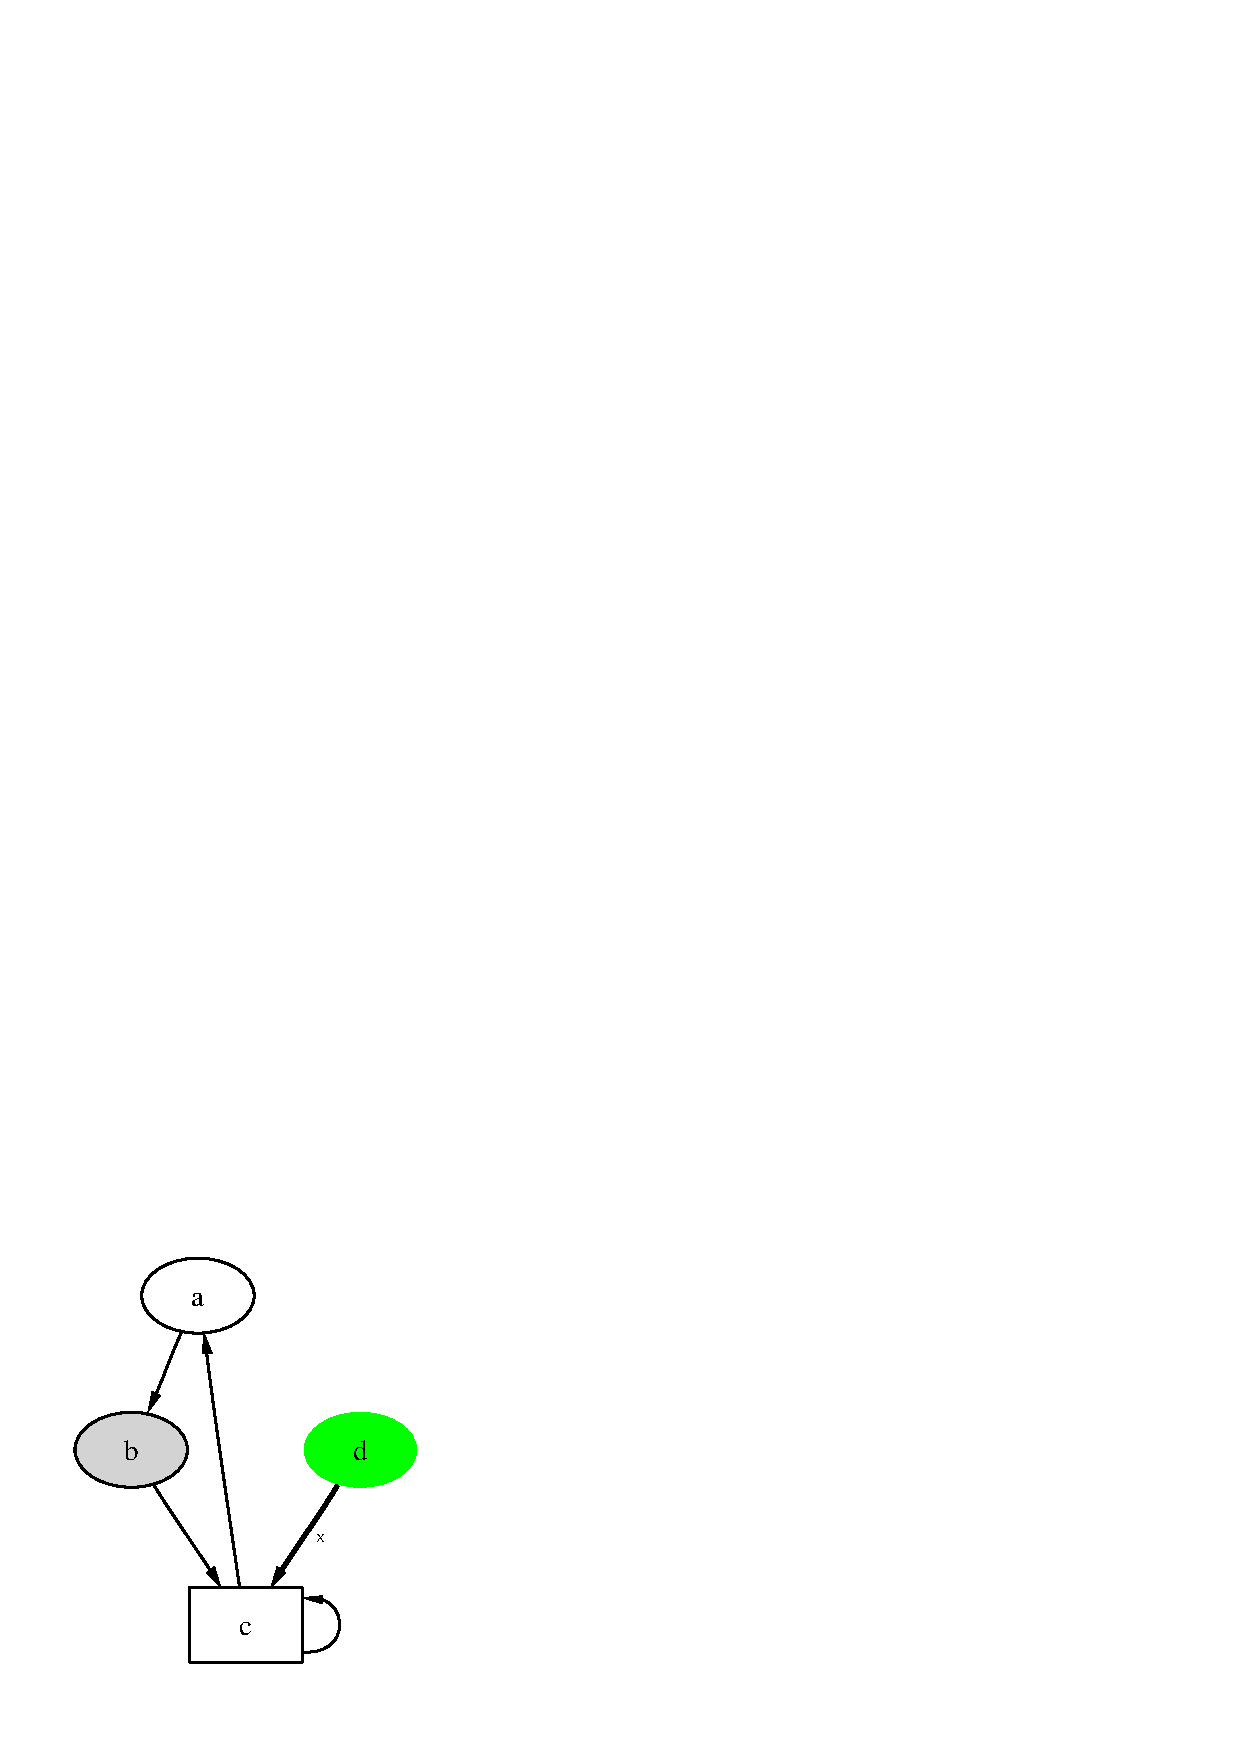
\epsfig{file = example.pdf, width = 4.5cm}
\end{center}
\caption{Un grafo generato con dot.}\label{fig:dot_example}
\end{figure}
%
Il linguaggio dot (\texttt{http://www.graphviz.org/}) permette di
disegnare grafi a partire da una loro specifica testuale data in
termini di nodi e archi fra nodi. Si consideri per esempio il grafo
in Figura~\ref{fig:dot_example}. Esso \`e stato generato a partire dal
seguente file sorgente \texttt{example.dot}, scritto nel linguaggio dot:
%
\begin{verbatim}
  digraph example {
    size = "11,7.5"

    a [label = "a"]
    b [label = "b" style = filled]
    c [label = "c" shape = box]
    d [label = "d" color = green style = filled]

    a -> b
    b -> c
    c -> c
    c -> a
    d -> c [label = "X" fontsize = 6 style = bold]
  }
\end{verbatim}
%
In tale sorgente si specificano, in un qualsiasi ordine, i nodi e
gli archi del grafo. Nodi e archi possono avere propriet\`a espresse fra
parentesi quadre per specificarne la forma, lo spessore o il colore.
La trasformazione di tale file sorgente nel file postscript in
Figura~\ref{fig:dot_example} avviene tramite il comando:
%
\begin{verbatim}
  dot -Tps example.dot >example.ps
\end{verbatim}
%
Ulteriori esempi sono presenti nella pagina web di dot.
\`E possibile avere ulteriori informazioni su dot anche tramite
il manuale in linea: \texttt{man dot}.

Adesso che abbiamo capito come si specifica un grafo tramite il linguaggio
dot, poniamoci il problema di generare un file sorgente dot a partire da una
classe di sintassi astratta che descrive una parte di codice Kitten.
Per esempio, la sintassi concreta
\texttt{!this.state} in Figura~\ref{fig:led} \`e tradotta nel sottoalbero
di sintassi astratta radicato in \texttt{Not} in Figura~\ref{fig:led_albero}.
Tale sottoalbero \`e specificato da un file sorgente dot del tipo:
%
\begin{verbatim}
  node19 [label = "Not"]
  node18 [label = "FieldAccess"]
  node17 [label = "Variable"]
  symbol_this [label = "this" fontname = "Times-Italic" shape = box]
  node17 -> symbol_this [label = "name" fontsize = 8]
  node18 -> node17 [label = "receiver" fontsize = 8]
  symbol_state [label = "state" fontname = "Times-Italic" shape = box]
  node18 -> symbol_state [label = "name" fontsize = 8]
  node19 -> node18 [label = "expression" fontsize = 8]
\end{verbatim}
%
Si noti che l'esatta numerazione dei nodi non \`e importante, a differenza
della loro etichetta che apparir\`a nel file postscript finale.
Quello che importa per\`o \`e che tale numerazione generi stringhe diverse
per nodi di sintassi astratta diversi, anche se poi la loro etichetta esterna,
quella visualizzata nel file postscript,
pu\`o coincidere. A tal fine, basta che ogni nodo di sintassi
astratta contribuisca al file dot con un nodo chiamato \texttt{node}$n$,
dove $n$ \`e l'identificatore unico di tale nodo (si veda il campo
\texttt{identifier} in Figura~\ref{fig:absyn.Absyn}). I simboli sono
invece condivisi e mai ripetuti (Figura~\ref{fig:symbol.Symbol}).
Essi saranno quindi rappresentati da un nodo chiamato \texttt{symbol\_}$x$,
dove $x$ \`e l'identificatore del simbolo.

La generazione del file sorgente dot \`e fatta con un algoritmo
a discesa ricorsiva:
un nodo di sintassi astratta genera una parte del file
che descrive se stesso e gli archi verso i suoi figli; quindi chiama
ricorsivamente la generazione della parte di file per i suoi figli.
Per esempio, il file precedente viene generato in questo modo:
il nodo \texttt{Not} genera le righe
%
\begin{verbatim}
  node19 [label = "Not"];
  node19 -> node18 [label = "expression" fontsize = 8]
\end{verbatim}
%
Quindi il nodo figlio di \texttt{Not}, \cioe un \texttt{FieldAccess},
genera le righe
%
\begin{verbatim}
  node18 [label = "FieldAccess"];
  node18 -> node17 [label = "receiver" fontsize = 8]
  node18 -> symbol_state [label = "name" fontsize = 8]
\end{verbatim}
%
I due nodi figli di \texttt{FieldAccess} sono una \texttt{Variable}, che
genera
%
\begin{verbatim}
  node17 [label = "Variable"];
  node17 -> symbol_this [label = "name" fontsize = 8]
\end{verbatim}
%
e un \texttt{Symbol}, che genera
%
\begin{verbatim}
  symbol_state [label = "state" fontname = "Times-Italic" shape = box]
\end{verbatim}
%
Infine, il figlio di \texttt{Variable} \`e un \texttt{Symbol} che genera
%
\begin{verbatim}
  symbol_this [label = "this" fontname = "Times-Italic" shape = box]
\end{verbatim}

Sebbene sia possibile dare una definizione formale della generazione
del file dot, limitiamoci per semplicit\`a a mostrarne l'implementazione Java.
Per prima cosa, aggiungiamo alcuni metodi di utilit\`a alla classe
\texttt{absyn/Absyn.java}. Questi sono mostrati in
Figura~\ref{fig:absyn.Absyn_dot}.
\begin{itemize}
\item Il metodo \texttt{label()} restituisce
l'etichetta che deve essere visualizzata dentro il nodo dot che
rappresenta un nodo di sintassi astratta. Normalmente, si tratta del
nome della classe di sintassi astratta, senza il prefisso che indica il
package \texttt{absyn} (per questo si usa \texttt{getSimpleName()}
piuttosto che \texttt{getName()}). Si noti che le sottoclassi potrebbero
ridefinire questo metodo. Per esempio, le classi per i letterali
ridefiniscono questo metodo in modo da specificare anche il valore lessicale
del letterale.
\item Il metodo \texttt{dotNodeName()} restituisce il nome usato nel file dot
per fare riferimento a un nodo di sintassi astratta. Come detto, si tratta
della stringa \texttt{node}$n$ dove $n$ \`e l'identificatore unico del
nodo di sintassi astratta.
\item Il metodo \texttt{linkToNode()} scrive dentro un file testo il comando
dot che crea un arco fra il nodo \texttt{this} di sintassi astratta e un
nodo di sintassi astratta il cui nome usato nel file dot \`e \texttt{to}.
Occorre anche specificare l'etichetta \texttt{name} dell'arco.
\item Il metodo \texttt{boldLinkToNode()} si comporta come
\texttt{linkToNode()} ma crea un arco di maggiore spessore. Questo
metodo \`e usato solo per legare un comando o un membro di una classe
al suo successore (campi \texttt{next}). Si veda per esempio la
Figura~\ref{fig:led_albero}.
\end{itemize}
%
\begin{figure}[t]
\begin{verbatim}
protected String label() {
  return this.getClass().getSimpleName();
}

protected final String dotNodeName() {
  return "node" + identifier;
}

protected final void linkToNode(String name, String to, FileWriter where)
{
  where.write(dotNodeName() + " -> " + to +
              " [label = \"" + name + "\" fontsize = 8]\n");
}

protected final void boldLinkToNode
  (String name, String to, FileWriter where)
{
  where.write(dotNodeName() + " -> " + to +
              " [label = \"" + name + "\" fontsize = 8 style = bold]\n");
}
\end{verbatim}
\caption{Metodi aggiunti alla classe \texttt{absyn/Absyn.java} in Figura~\ref{fig:absyn.Absyn} per la generazione della rappresentazione dot della sintassi astratta.}
  \label{fig:absyn.Absyn_dot}
\end{figure}

A questo punto possiamo definire un metodo ricorsivo per la generazione del
file dot a partire da un nodo di sintassi astratta. Lo chiameremo
\texttt{toDot()}. La sua intestazione \`e:
%
\begin{verbatim}
  public String toDot(FileWriter where)
\end{verbatim}
%
Questo significa che il metodo scrive dentro il file indicato il codice
dot che rappresenta la classe di sintassi astratta e i suoi figli (e
ricorsivamente i figli dei figli\ldots). Il valore
di ritorno \`e il nome usato nel file dot per rappresentare il nodo
di sintassi astratta su cui il metodo \`e invocato.

Cominciamo dai tipi. Il metodo \texttt{toDot()} \`e \cosi definito in
\texttt{absyn/TypeExpression.java}:
%
\begin{verbatim}
  public final String toDot(FileWriter where) {
    where.write(dotNodeName() + " [ label = \"" + label() + "\"];\n");
    toDot$0(where);
    return dotNodeName();
  }

  protected void toDot$0(FileWriter where) {}
\end{verbatim}
%
Si noti che \texttt{toDot()}
\`e definito come \texttt{final}. Esso si limita a generare
un nodo dot per il nodo di sintassi astratta e a chiamare un metodo ausiliario
\texttt{protected} che di default non fa nulla. Le ridefinizioni del
metodo \texttt{toDot\$0()} creano degli archi
verso i nodi figli e richiamano ricorsivamente \texttt{toDot()}.
Per esempio, eccone la ridefinizione dentro
\texttt{absyn/ArrayTypeExpression.java}:
%
\begin{verbatim}
  protected void toDot$0(FileWriter where) {
    linkToNode("elementsType",elementsType.toDot(where),where);
  }
\end{verbatim}
%$

Lo stesso procedimento si usa per le espressioni.
La definizione di \texttt{toDot()} dentro alla classe
\texttt{absyn/Expression.java} \`e
identica al caso dei tipi. La ridefinizione di \texttt{toDot\$()} dentro
\texttt{absyn/Variable.java} \`e per esempio
%
\begin{verbatim}
  protected void toDot$0(FileWriter where) {
    linkToNode("name",name.toDot(where),where);
  }
\end{verbatim}
%$
e quella dentro \texttt{absyn/FieldAccess.java} \`e:
%
\begin{verbatim}
  protected void toDot$0(FileWriter where) {
    linkToNode("receiver",receiver.toDot(where),where);
    linkToNode("name",name.toDot(where),where);
  }
\end{verbatim}
%$
Come altro esempio, la ridefinizione di \texttt{toDot\$0()} dentro
\texttt{absyn/BinOp.java} \`e
%
\begin{verbatim}
  protected void toDot$0(FileWriter where) {
    linkToNode("left",left.toDot(where),where);
    linkToNode("right",right.toDot(where),where);
  }
\end{verbatim}
%$

Vediamo infine la definizione di \texttt{toDot()} dentro
\texttt{symbol/Symbol.java} (Figura~\ref{fig:symbol.Symbol}):
%
\begin{verbatim}
  public String toDot(FileWriter where) {
    where.write("symbol_" + name +
                " [label = \"" + name + "\"" +
                " fontname = \"Times-Italic\" shape = box]\n");
    return "symbol_" + name;
  }
\end{verbatim}
%
Questa volta il metodo genera un nodo dot di nome \texttt{symbol\_}$x$,
dove $x$ \`e il nome del simbolo. I simboli non hanno mai archi uscenti, per
cui costituiscono un caso base della discesa ricorsiva (le foglie
dell'albero in Figura~\ref{fig:led_albero}).

La definizione di \texttt{toDot()} \`e simile per i comandi. Per la
struttura complessiva di una classe, il metodo \texttt{toDot()}
si richiama ricorsivamente sui componenti della classe e aggiunge al file
dot un prologo che specifica la dimensione della pagina e un epilogo, \cioe
la parentesi graffa di chiusura!
%
\javatip{
L'aggiunta di una nuova classe di sintassi astratta al compilatore
Kitten comporta
la definizione del suo metodo \texttt{toDot\$0()}. Come visto in questi
esempi, si tratta semplicemente di una sequenza di
chiamate a \texttt{linkToNode()} per ciascuno dei figli della classe
di sintassi astratta che \`e stata aggiunta. In assenza della specifica
del metodo
\texttt{toDot\$0()}, il comportamento di default sar\`a quello dell'omonimo
metodo, vuoto, definito in \texttt{absyn/TypeExpression.java} per i tipi,
\texttt{absyn/Expression.java} per le espressioni e
\texttt{absyn/Command.java} per i comandi. Conseguentemente non sar\`a
visibile, nel file postscript generato da dot, il sottoalbero
radicato nei nodi di sintassi astratta per la nuova classe che \`e
stata aggiunta. Un comportamento indesiderato che non finisce
di meravigliare gli studenti\ldots}
%
\begin{exercise}\label{ex:descent_fields}
Si formalizzi uno schema a discesa ricorsiva che calcola l'insieme dei
nomi di campi letti in un comando. Si faccia lo stesso per l'insieme
dei nomi delle classi istanziate in un comando.
\end{exercise}
%
\begin{exercise}\label{ex:expressions_simplify}
Si definisca con una discesa ricorsiva un giudizio
$\vdash^{\mathsf{simp}}$ tale che
$\mathit{exp}\vdash^{\mathsf{simp}}\mathit{exp}'$ \`e vero quando
l'espressione Kitten $\mathit{exp}'$ \`e ottenuta \emph{semplificando}
un'altra espressione Kitten $\mathit{exp}$. La semplificazione da considerare
\`e quella che sostituisce operazioni binarie fra costanti numeriche
con il loro risultato. Una costante numerica \`e un letterale numerico
o un'operazione binaria aritmetica fra costanti numeriche.
Si schematizzi quindi l'implementazione Java di $\vdash^{\mathsf{simpl}}$.
Riportiamo sotto alcuni esempi di coppie $\mathit{exp}$ ed $\mathit{exp}'$:
%
\[
{\scriptsize
\begin{array}{|c|c|}\hline
  \mathit{exp} & \mathit{exp'}\\\hline\hline
  \mathtt{Addition(IntLiteral(4),IntLiteral(5))} & \mathtt{IntLiteral(9)} \\
    \hline
  \mathtt{LessThan(IntLiteral(4),IntLiteral(5))} & \mathtt{True()} \\\hline
  \mathtt{Addition(Multiplication(IntLiteral(4),IntLiteral(5)),
    Variable(x))} & \mathtt{Addition(IntLiteral(20),Variable(x))}\\\hline
\end{array}
}
\]
\end{exercise}

\chapter{Analisi Semantica}\label{chap:semantical}
%
\vspace*{-2ex}
\begin{center}
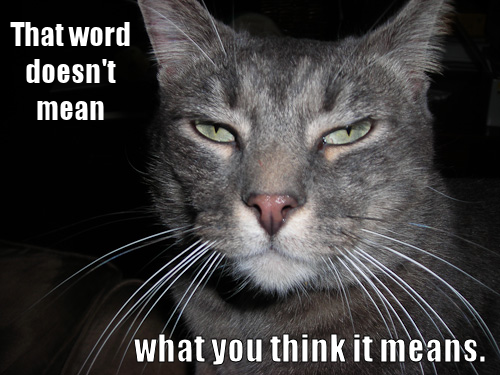
\includegraphics[width=6.5cm]{ThinkingCat.png}
\end{center}
%\vspace*{-2ex}
%
Le analisi lessicale e sintattica dei Capitoli~\ref{chap:lexical}
e~\ref{chap:syntactical} garantiscono che il programma sorgente
soddisfi le regole di sintassi specificate, rispettivamente,
da un insieme di token e da una grammatica. L'analisi sintattica
ha inoltre costruito un albero di sintassi astratta che fornisce una visione
strutturata del file sorgente (Figura~\ref{fig:led_albero}).
Questo non significa che tutti i programmi che hanno superato con successo
l'analisi sintattica, \cioe senza generare alcun errore di sintassi,
siano automaticamente dei programmi \emph{corretti}, pronti a essere tradotti
in codice oggetto ed eseguiti. Per esempio, basta prendere il programma
della Figura~\ref{fig:led} e modificare la linea \texttt{this.state := true}
in \texttt{this.state := 3} per ottenere un programma che supera senza alcun
problema sia l'analisi lessicale che quella sintattica, ma che non \`e
\emph{corretto}, poich\'e esso tenta di assegnare un valore intero
($3$) a un campo che pu\`o contenere solo valori di tipo
booleano (\texttt{state}). Accorgersi di tali errori va ben al di l\`a delle
possibilit\`a delle grammatiche libere dal contesto. Serve uno strumento
alternativo, ovvero quello della discesa ricorsiva sull'albero di sintassi
astratta del codice sorgente, alla ricerca di errori \emph{semantici}
nel codice. Questa \emph{analisi semantica} \e l'oggetto di questo capitolo.

Pi\`u in dettaglio, i compiti di un'analisi semantica sono quelli di
%
\begin{enumerate}
\item costruire una rappresentazione (una struttura dati) che descrive
      i tipi usati dal programma (tipi primitivi ma anche array e classi);
\item identificare usi di espressioni incompatibili con i loro tipi statici
      (\emph{errori di tipo});
\item identificare occorrenze di variabili usate ma non dichiarate;
%\item garantire che i comandi \texttt{break} e \texttt{continue} occorrano
%      solo nello scope di un'istruzione iterativa;
\item garantire che un metodo non \texttt{void} termini sempre con
      un comando \texttt{return} \textit{exp},
      indipendentemente dal percorso di
      esecuzione che viene seguito al suo interno, e che un metodo
      \texttt{void} non contenga comandi di tipo \texttt{return} \textit{exp};
\item garantire che non ci siano parti di codice che non possono mai
      essere eseguite e che sono quindi irraggiungibili e \emph{inutili}
      (identificazione \emph{del codice morto});
\item identificare e annotare il tipo statico delle espressioni che occorrono
      in un programma (\emph{inferenza dei tipi});
\item identificare, per ogni accesso a un campo, la classe in cui il campo
      \`e definito;
\item identificare, per ogni istruzione \texttt{new} \textit{Classe},
      il costruttore di \textit{Classe}
      che deve essere chiamato in tale punto a tempo di esecuzione,
      sulla base del tipo statico dei parametri attuali;
\item identificare, per ogni invocazione di metodo,
      la dichiarazione del metodo
      che deve essere chiamato (o una cui ridefinizione deve essere chiamata)
      in tal punto a tempo di esecuzione,
      sulla base del tipo statico dei parametri attuali.
\end{enumerate}
%
Potremmo quindi dire che l'analisi semantica si occupa di
costruire una rappresentazione dei tipi usati dal programma (punto 1)
che viene poi usata per garantire condizioni
di correttezza elementari, senza le quali non ha neppure senso compilare
il programma in codice oggetto (\emph{verifica del codice},
punti 2--5) e per raccogliere informazione
sul programma che si sta compilando, al fine di facilitare la successiva
fase di generazione del codice oggetto (\emph{annotazione del codice},
punti 6--9). Va detto che tale
divisione \`e concettualmente utile ma non netta, dal momento che, per
esempio, l'identificazione del costruttore chiamato da un'istruzione
\texttt{new} (punto 8) \`e s\`{\i} un'annotazione utile a
generare il codice oggetto
che effettua la chiamata a tale costruttore, ma \`e anche una verifica che
tale costruttore esista realmente. L'insieme esatto
dei compiti affidati all'analisi semantica varia comunque molto da
linguaggio a linguaggio.
Altre verifiche effettuate da Java \emph{ma non da Kitten} sono per esempio:
%
\begin{enumerate}
\item[10.] garantire che i comandi \texttt{break} e \texttt{continue}
           occorrano solo dentro un costrutto iterativo o, per il solo
           \texttt{break}, dentro un comando \texttt{switch};
\item[11.] garantire che l'uso di una variabile locale trovi la variabile
           inizializzata, indipendentemente dal percorso di esecuzione
           che ha portato al punto di utilizzo della variabile\footnote
           {In Kitten una variabile va inizializzata al momento
           della sua dichiarazione, per cui questo controllo \e inutile.}.
\end{enumerate}
%
\section{I tipi Kitten}\label{sec:semantical_types}
%
Il concetto di \emph{tipo} (Sezione~\ref{sec:types}) \`e al centro
dell'analisi semantica (punti 1,2,4,6,8,9 della precedente
enumerazione). Va subito notato che per \emph{tipo}
non intendiamo qui la sintassi
astratta di una \emph{espressione} di tipo, come nella
Sezione~\ref{subsec:types_abstract}. In quel contesto avevamo bisogno di
un modo per rappresentare la \emph{struttura sintattica} di una parte di codice
che rappresentava un tipo Kitten. Si tratta invece adesso di rappresentare
la \emph{struttura semantica} dei tipi delle espressioni Kitten,
\cioe una struttura dati con associate alcune operazioni
che permettono, per esempio, di determinare se un tipo \`e un sottotipo
di un altro o qual \`e il minimo supertipo
comune fra due o \piu tipi, se esso esiste (Sezione~\ref{sec:types}), o quali
siano i campi o i costruttori o metodi di un tipo classe.
Per apprezzare la differenza, basta osservare che
due occorrenze dell'espressione \texttt{int} in due punti diversi
di un file sorgente danno origine a due oggetti \texttt{IntTypeExpression}
diversi, ma il loro tipo semantico \`e lo stesso identico oggetto.

La distribuzione Kitten contiene il package \texttt{types}, al cui interno
trovano posto delle classi che rappresentano i tipi \emph{semantici}
del linguaggio Kitten.
%
\begin{figure}
\begin{center}
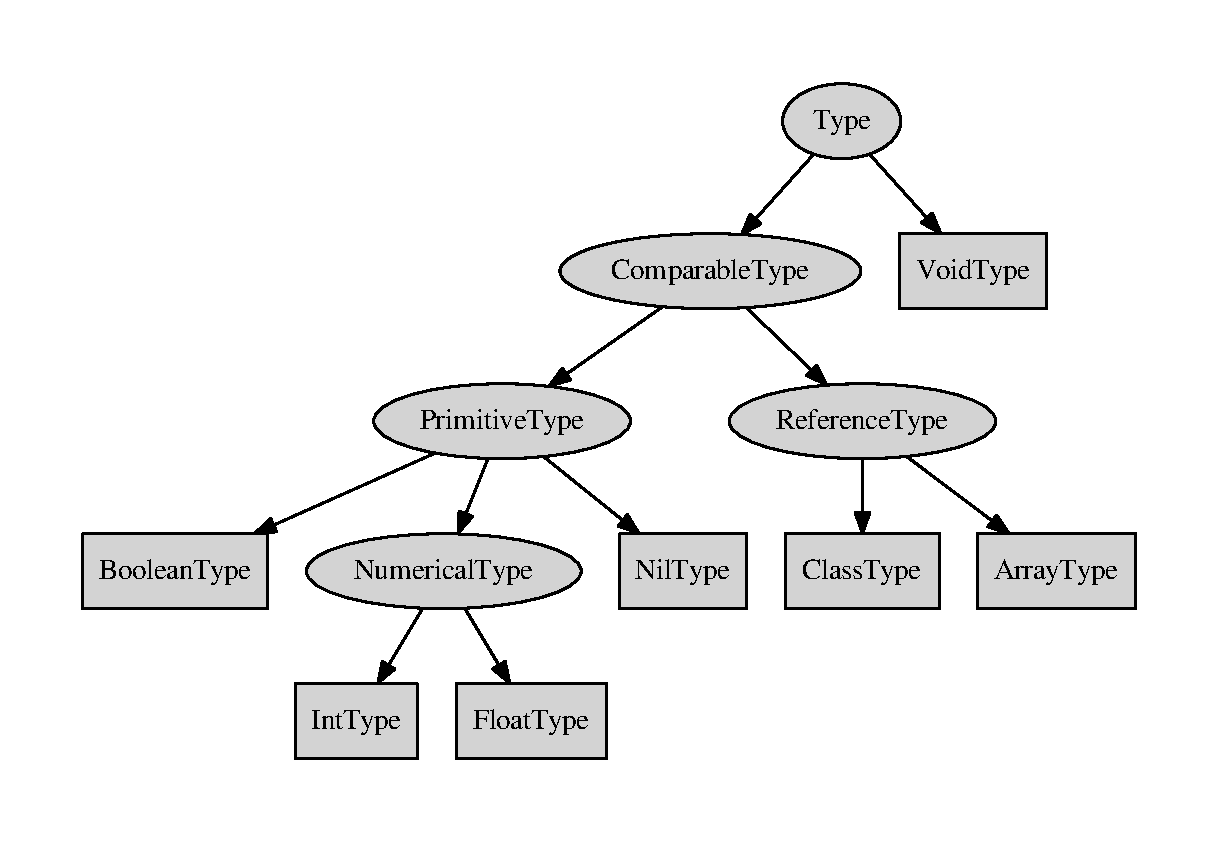
\includegraphics[width=12cm]{semantical_types.pdf}
\end{center}
\caption{Le classi del package \texttt{types} che rappresentano i tipi semantici di Kitten.}\label{fig:semantical_types}
\end{figure}
%
La Figura~\ref{fig:semantical_types} presenta la gerarchia di tali classi.
I tipi sono in primo luogo divisi fra \emph{confrontabili} e \texttt{void}.
I tipi confrontabili sono quelli per i cui valori \`e definito almeno
l'operatore di confronto \texttt{=}. Essi sono a loro volta divisi fra
tipi \emph{primitivi} e \emph{riferimento} (Sezione~\ref{sec:types}). I tipi
\emph{numerici} sono quei tipi primitivi che rappresentano numeri e per
cui sono definite le usuali operazioni di confronto, come il \texttt{<},
oltre a \texttt{=}.
Si noti che non esiste un tipo specifico per le stringhe, che sono invece
considerate come un caso di \texttt{ClassType}.

La Figura~\ref{fig:types.Type} mostra l'implementazione della superclasse
\texttt{types/Type.java}. Le sue sottoclassi dovranno istanziare
il metodo \texttt{canBeAssignedTo()} che determina
se un tipo pu\`o essere assegnato a un
altro, seguendo le regole che nella Sezione~\ref{sec:types}
hanno portato alla definizione della relazione $\le$ sui tipi. Il metodo
\texttt{canBeAssignedToSpecial()} \e per default un sinonimo di
\texttt{canBeAssignedTo()}, ma viene ridefinito in
\texttt{types/PrimitiveType.java} e \texttt{types/Void.java} come segue:
%
\begin{verbatim}
  public boolean canBeAssignedToSpecial(Type other) {
    return this == other;
  }
\end{verbatim}
%
in modo che i tipi primitivi e \texttt{void} siano
\emph{sottotipo speciale} solo di se stessi. Questo metodo \`e
utile all'interno della classe \texttt{ArrayType}, che vedremo fra un attimo,
per implementare la relazione di sottotipaggio $\le$ che come sappiamo
non \`e monotona sugli array di tipi primitivi (Sezione~\ref{sec:types}).
Esso \e usato anche per determinare se il tipo di ritorno di una ridefinizione
di un metodo \`e compatibile con quello del metodo ridefinito.
Il metodo \texttt{leastCommonSupertype()} determina il minimo supertipo comune
fra due tipi. Tale supertipo potrebbe non esistere: per esempio, fra
\texttt{int} e \texttt{boolean} non c'\e alcun supertipo comune.
La definizione fornita dentro
\texttt{types/Type.java} funziona per tutti i tipi primitivi, ma come
vedremo deve essere ridefinita per i tipi riferimento.
Si noti che il costruttore di \texttt{types/Type.java} \`e \texttt{protected}.
Anche i costruttori delle altre classi che implementano i tipi semantici sono
\texttt{protected} o \texttt{private}. Quindi
l'unico modo per ottenere degli oggetti della
gerarchia in Figura~\ref{fig:semantical_types} sar\`a tramite le costanti
presenti dentro ciascuna classe (per esempio, \texttt{types/IntType.INSTANCE})
o tramite dei metodi statici con memoria che
definiremo dentro le classi per i tipi riferimento. Questo implica
che \emph{esiste al pi\`u un oggetto per un dato tipo semantico}
e l'uguaglianza fra tipi pu\`o essere controllata con
semplici confronti Java \texttt{==}. Si tratta di un esempio di applicazione
del design pattern del \emph{singleton}, esteso a tutte le possibili istanze
di una classe. Il metodo \texttt{getObjectType()}
ritorna il tipo della superclasse \texttt{Object} di tutte le classi e array.

\begin{figure}[t]
{\small
\begin{verbatim}
public abstract class Type {

  protected Type() {}

  public abstract boolean canBeAssignedTo(Type other);

  public boolean canBeAssignedToSpecial(Type other) {
    return canBeAssignedTo(other); // i tipi primitivi e void lo ridefiniscono
  }

  public Type leastCommonSupertype(Type other) {
    // questo e' ok per i tipi primitivi. Classi e array lo ridefiniscono
    if (this.canBeAssignedTo(other)) return other;
    else if (other.canBeAssignedTo(this)) return this;
    else return null; // non esiste
  }

  public static final ClassType getObjectType() { ... ritorna il tipo per Object }
}
\end{verbatim}
}
\caption{La superclasse astratta dei tipi semantici di Kitten}
  \label{fig:types.Type}
\end{figure}

Si consideri la classe \texttt{types/IntType.java}
in Figura~\ref{fig:types.IntVoidType}.
Come si vede, ammettiamo che il tipo \texttt{int} sia assegnato a
\texttt{int} stesso ma anche a \texttt{float}, poich\'e
$\mathtt{int}\le\mathtt{float}$ (Sezione~\ref{sec:types}).
La classe \texttt{types/VoidType.java} \`e simile, ma non ammettiamo
l'assegnamento verso nessun tipo, neppure \texttt{void}.
L'assegnamento speciale \`e invece possibile ma solo verso \texttt{void}
stesso, come abbiamo gi\`a detto.
%
\begin{figure}
{\small
\begin{verbatim}
           public class IntType extends NumericalType {
             protected IntType() {}
             public boolean canBeAssignedTo(Type other) {
               return other == IntType.INSTANCE || other == FloatType.INSTANCE;
             }
           }

           public class VoidType extends Type {
             protected VoiType() {}
             public boolean canBeAssignedTo(Type other) { return false; }
             public boolean canBeAssignedToSpecial(Type other) {
                 return this == other;
             }
           }
\end{verbatim}}
\caption{Le classi \texttt{types/IntType.java} e
         \texttt{types/VoidType.java} che implementano rispettivamente i tipi
         \texttt{int} e \texttt{void}.}
  \label{fig:types.IntVoidType}
\end{figure}

\greycomment{
La scelta di imporre l'uguaglianza nella relazione di sottotipo speciale
per i tipi primitivi ha l'effetto che, nel controllo di compatibilit\`a
del tipo di ritorno della ridefinizione di un metodo, un tipo primitivo pu\`o
essere solo sottotipo di se stesso. Si osservi che se \texttt{float m()}
potesse essere ridefinito, in una sottoclasse, in \texttt{int m()}
allora una chiamata virtuale del tipo \texttt{float f = o.m()} richiederebbe,
o meno, una conversione di tipo da \texttt{int} a \texttt{float} sulla base
della classe, a tempo di esecuzione, dell'oggetto contenuto in \texttt{o}, il
che complica la generazione del codice. Per questo motivo impediamo al programmatore di
fare una simile ridefinizione del tipo di ritorno del metodo \texttt{m()}.
Questo stesso vincolo \e imposto nel linguaggio Java.}

\begin{figure}[t]
{\small
\begin{verbatim}
public class ArrayType extends ReferenceType {
  private final Type elementsType;
  private ArrayType(Type elementsType) { this.elementsType = elementsType; }
  public static ArrayType mk(Type elementsType) {
    ... usa una memoria per non ricreare tipi array gia' creati in passato
  }
  public boolean canBeAssignedTo(Type other) {
    if (other instanceof ArrayType)
      return elementsType.canBeAssignedToSpecial(((ArrayType) other).elementsType);
    else return other == getObjectType();
  }
  public Type leastCommonSupertype(Type other) {
    // l'lcs fra un array e una classe e' Object
    if (other instanceof ClassType) return getObjectType();
    else if (other instanceof ArrayType)
      if (elementsType instanceof PrimitiveType)
        // fra un array di tipi primitivi e se stesso l'lcs e' l'array.
        if (this == other) return this;
        // fra due array di tipi primitivi diversi, l'lcs e' Object
        else return getObjectType();
      else {
        Type lcs = elementsType.leastCommonSupertype(((ArrayType) other).elementsType);
        return lcs == null ? getObjectType() : mk(lcs);
      }
    else if (other == NilType.ISTANCE) return this; // fra un array e nil e' l'array
    else return null; // non esiste alcun lcs
  }
}
\end{verbatim}
}
\caption{La classe \texttt{types/ArrayType.java} che rappresenta i tipi array.}\label{fig:types.ArrayType}
\end{figure}

La classe \texttt{types/ArrayType.java} in Figura~\ref{fig:types.ArrayType}
implementa i tipi array. L'invariante che
non esistano istanze diverse dello stesso tipo \`e mantenuta rendendone
\texttt{private} il costruttore e permettendo la
creazione di tipi array solo tramite il metodo statico \texttt{mk()}, che
usa una memoria per evitare di creare duplicati.
L'assegnamento di un tipo array \texttt{this}
a un altro tipo \texttt{other} \`e considerata
legale solo se \texttt{other} \`e \texttt{Object} oppure se anche
\texttt{other} \e un tipo array e gli elementi di \texttt{this}
possono a loro volta essere assegnati a quelli di \texttt{other}.
Ma si noti l'uso di \texttt{canBeAssignedToSpecial()} per questa chiamata
ricorsiva! Questo al fine di imporre il vincolo
della Sezione~\ref{sec:types} che richiede che se gli elementi
di \texttt{this} sono un tipo primitivo allora quelli di \texttt{other} devono
essere \emph{lo stesso} tipo primitivo.
%
\greycomment{Questo vincolo, apparentemente strano, \`e giustificato dal fatto
che, se \texttt{arr} \`e un array di interi, allora
il comando \texttt{int[] copy := arr}
rende \texttt{arr} e \texttt{copy} \emph{alias}, \cioe riferimenti diversi
allo stesso oggetto array. Mentre il comando \texttt{float[] copy := arr}
ci impone di convertire ciascun elemento di \texttt{arr} da \texttt{int}
a \texttt{float}. Dal momento che dobbiamo lasciare immutato l'array
\texttt{arr}, la conversione \`e possibile solo a costo di creare
un \emph{nuovo} array di \texttt{float} che contiene i valori convertiti.
Tale array verrebbe poi assegnato a \texttt{copy}. Ma questo significa
che \texttt{arr} e \texttt{copy} non sarebbero \piu alias! Detto
altrimenti, la scelta del tipo degli elementi di \texttt{copy} determinerebbe
la condivisione (o meno) fra \texttt{arr} e \texttt{copy}. Tale comportamento,
nettamente inaspettato dal programmatore, \`e da considerarsi
semanticamente pericoloso ed
\`e quindi conveniente vietare tali assegnamenti. Va notato inoltre che il
costo computazionale dell'assegnamento diventerebbe lineare nella lunghezza
dell'array piuttosto che costante, come normalmente si richiede.}

Il metodo \texttt{leastCommonSupertype()} di
\texttt{ArrayType} deve determinare il minimo supertipo comune
(\emph{lcs}) fra il tipo array \texttt{this} e un altro tipo \texttt{other}.
Le regole che portano alla definizione di \emph{lcs} sono le seguenti:
%
\begin{itemize}
\item se \texttt{other} \`e una classe allora \emph{lcs} \`e \texttt{Object}.
      Si noti infatti che tutti gli array e tutte le classi sono
      sottotipi di \texttt{Object} (Sezione~\ref{sec:types});
\item se anche \texttt{other} \`e un tipo array allora:
      \begin{itemize}
      \item se entrambi sono array dello stesso tipo primitivo
            allora \emph{lcs} \`e uguale
            a \texttt{this} (o equivalentemente a \texttt{other});
      \item se entrambi sono array di tipi primitivi, ma diversi,
            allora \emph{lcs} \`e \texttt{Object}\footnote{Si noti che sarebbe
            errato definire in questo caso \emph{lcs} come
            \texttt{array of Object}, poich\'e i tipi primitivi non sono
            sottotipi di \texttt{Object}};
      \item se entrambi sono array di tipi non primitivi
            allora \emph{lcs} \`e il tipo array del minimo supertipo comune
            fra i tipi degli elementi di \texttt{this} e \texttt{other};
      \end{itemize}
\item se \texttt{other} \`e il tipo \texttt{NilType}, allora
      \emph{lcs} \`e \texttt{this} poich\'e \texttt{NilType} \`e un
      sottotipo di qualsiasi tipo array (Sezione~\ref{sec:types});
\item altrimenti \emph{lcs} non esiste.
\end{itemize}

\begin{figure}[t]
{\scriptsize
\begin{verbatim}
public class ClassType extends ReferenceType {
  private String name;                    // il nome di questa classe
  private ClassType superclass;           // la sua superclasse (se esiste)
  private List<ClassType> subclasses;     // le sue sottoclassi (se esistono)
  private ClassDefinition abstractSyntax; // la sintassi astratta della classe

  private ClassType(String name) {
    ... salva this nella memoria usata da mk()
    this.name = name;
    Parser parser = new Parser(new Lexer(name));
    (abstractSyntax = (ClassDefinition) parser.parse().value).addMembersTo(this);
    if (!name.equals("Object")) {
      superclass = mk(abstractSyntax.getSuperclassName());
      superclass.subclasses.add(this);
    }
  }
  public static ClassType mk(String name) {
    ... restituisci l'eventuale classe di nome name contenuta nella memoria
    ... altrimenti restituisci new ClassType(name)
  }
  public FieldSignature fieldLookup(String name) { ... }
  public ConstructorSignature constructorLookup(TypeList formals) { ... }
  public Set<ConstructorSignature> constructorsLookup(TypeList formals) { ... }
  public MethodSignature methodLookup(String name, TypeList formals) { ... }
  public Set methodsLookup(String name, TypeList formals) { ... }
  public boolean canBeAssignedTo(Type other) {
    return other instanceof ClassType && this.subclass((ClassType) other);
  }
  public boolean subclass(ClassType other) {
    return this == other || (superclass != null && superclass.subclass(other));
  }
  public Type leastCommonSupertype(Type other) {
    if (other instanceof ArrayType) return getObjectType();
    else if (other instanceof ClassType)
      for (ClassType cursor = this; ; cursor = cursor.superclass)
        if (other.canBeAssignedTo(cursor)) return cursor;
    return other == NilType.INSTANCE ? this : null;
  }
}
\end{verbatim}
}
\caption{La classe \texttt{types/ClassType.java} che implementa il tipo classe di Kitten.}
  \label{fig:types.ClassType}
\end{figure}

Vediamo infine il tipo \texttt{ClassType}, che rappresenta i tipi
classe come \texttt{Object},
\texttt{String} o \texttt{Led} in Figura~\ref{fig:led}. La
Figura~\ref{fig:types.ClassType} ne riporta il codice. Il costruttore
\`e lasciato \texttt{private} e la costruzione di tipi classe \`e
possibile solo tramite il metodo statico \texttt{mk()} che ne garantisce
l'unicit\`a. Il costruttore si occupa di creare un analizzatore lessicale per
il file sorgente della classe, interfacciarlo con un analizzatore sintattico
ed effettuare il parsing sintattico della classe. La sintassi astratta \cosi
costruita \e memorizzata nel tipo classe. La costruzione prosegue con la
superclasse, di cui il nuovo oggetto diventa una sottoclasse.
Se non esistesse nessun file col nome della classe seguito
da \texttt{.kit} o se tale file contenesse degli errori di sintassi,
il metodo \texttt{parse()} del parser fallirebbe senza restituire alcuna
sintassi astratta. Tale eccezione sarebbe allora
intercettata da un gestore di eccezioni (non mostrato in
Figura~\ref{fig:types.ClassType}) che fornisce alla classe
una sintassi astratta minimale (superclasse \texttt{Object}, nessun
campo, n\'e costruttori, n\'e metodi). In questo modo si evita di
bloccare la compilazione di un programma soltanto perch\'e una della sue classi
contiene un errore: si va avanti con la compilazione
finch\'e si pu\`o, segnalando quanti \piu errori possibile al programmatore.

Un tipo classe ha informazione sulla \emph{segnatura}
della classe, \cioe sui suoi campi, costruttori e metodi.
Questa informazione \e estratta dalla sua sintassi astratta al momento
della costruzione di un tipo classe tramite e aggiunta a quest'ultimo,
tramite il metodo \texttt{addMembersTo()} a discesa ricorsiva
(Figura~\ref{fig:types.ClassType}). Si noti che se
i campi, costruttori o metodi fanno riferimento alla stessa classe che
stiamo creando non entriamo in loop poich\'e abbiamo avuto cura di
registrare il tipo classe che stiamo creando nella memoria di
\texttt{mk()} prima di chiamare \texttt{addMembersTo()}.

La segnatura della classe pu\`o essere
consultata in seguito tramite dei metodi di ricerca (\emph{lookup}).
La differenza fra i metodi
\texttt{constructorLookup()} e \texttt{constructorsLookup()} \`e che il
primo cerca il costruttore con parametri formali esattamente identici a quelli
indicati, mentre il secondo fornisce l'insieme $S$ di
\emph{tutti} i costruttori con parametri
formali aventi tipi compatibili con quelli indicati.
\`E garantito il vincolo che
nessun costruttore in $S$ ha un altro costruttore in $S$ con parametri
formali \piu specifici dei suoi. Per esempio, nella segnatura della classe:
%
\begin{verbatim}
  class Ambiguous {
    constructor(int i, float d) {}
    constructor(float d, int i) {}
    /* constructor(int i1, int i2) {} */
  }
\end{verbatim}
%
il risultato di una chiamata a
\texttt{constructorsLookup()} avente come parametri una lista di
due \texttt{IntType} \`e l'insieme dei
due costruttori della classe non commentati.
Entrambi sono infatti compatibili con
due parametri di tipo \texttt{int}. Se si eliminasse il commento intorno
al terzo costruttore, la stessa chiamata a \texttt{constructorsLookup()}
restituirebbe un insieme formato dal solo
terzo costruttore, che \`e \piu specifico degli altri due.
Si pu\`o adesso comprendere a cosa ci servir\`a il metodo
\texttt{constructorsLookup()}:
di fronte a una invocazione del costruttore di \texttt{Ambiguous},
del tipo \texttt{new Ambiguous(3, 4)}, il compilatore Kitten
determiner\`a, tramite \texttt{constructorsLookup()}, l'insieme
dei possibili costruttori candidati a essere chiamati in tale punto di
programma. Se ce ne fosse \piu d'uno, la chiamata verrebbe considerato
\emph{ambigua}. Se non ce ne fosse nessuno, la
chiamata verrebbe considerata \emph{indefinita}.
In entrambi i casi essa verrebbe rifiutata in fase di analisi semantica
(lo vedremo quando commenteremo la Figura~\ref{fig:analysis_expressions2}).
Lo stesso discorso si pu\`o fare per
\texttt{methodLookup()} e \texttt{methodsLookup()}, con l'unica differenza che,
dal momento che Kitten implementa l'ereditariet\`a per campi e metodi,
la loro ricerca inizia in una data segnatura e,
se tale segnatura non definisce esplicitamente il campo o il metodo, la ricerca
prosegue ricorsivamente verso l'alto risalendo la catena delle estensioni,
verso \texttt{Object}.

Il metodo \texttt{canBeAssignedTo()} permette l'assegnamento verso la
stessa classe o una sua superclasse.
Il test di sottoclasse \`e realizzato dal metodo \texttt{subclass()}
che scorre verso l'alto a partire da \texttt{this}
la catena di estensione delle classi alla ricerca
dell'ipotetica superclasse.
Il metodo \texttt{leastCommonSupertype()} determina il minimo supertipo
comune \emph{lcs}
fra il tipo classe \texttt{this} e un altro tipo \texttt{other}
secondo le regole seguenti:
%
\begin{itemize}
\item se \texttt{other} \`e un tipo array, allora \emph{lcs} \`e
      \texttt{Object}, poich\'e tutte le classi e gli array sono
      sottotipi di \texttt{Object} (Sezione~\ref{sec:types});
\item se anche \texttt{other} \`e un tipo classe allora \emph{lcs}
      \`e la pi\`u specifica superclasse di \texttt{this} che \`e anche
      superclasse di \texttt{other}. Si noti che abbiamo la garanzia che
      tale \emph{lcs} esista poich\'e questa ricerca si ferma, nel
      peggiore dei casi, su \texttt{Object};
\item se \texttt{other} \`e il tipo \texttt{NilType}, allora
      \emph{lcs} \`e \texttt{this}, poich\'e \texttt{NilType} \`e
      sempre un sottotipo dei tipi classe (Sezione~\ref{sec:types});
\item altrimenti \emph{lcs} non esiste.
\end{itemize}
%
\begin{figure}[t]
\begin{center}
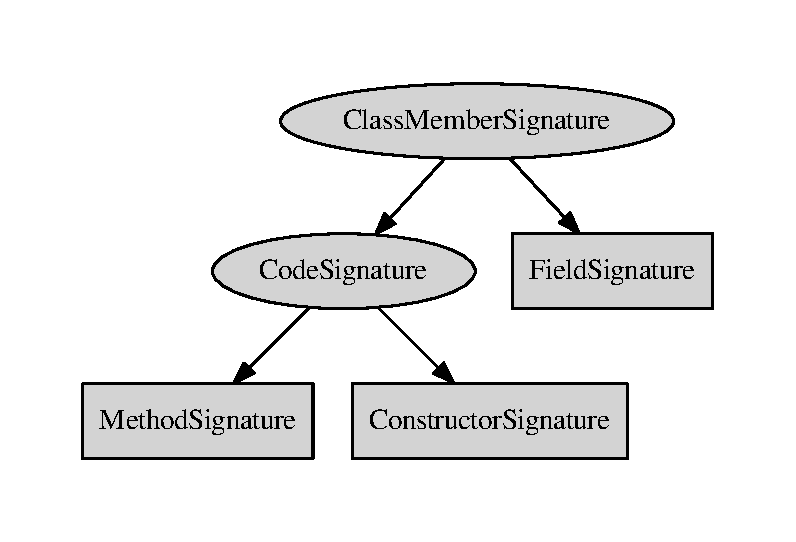
\includegraphics[width=9cm]{signatures_hierarchy.pdf}
\end{center}
\caption{Le classi del package \texttt{types} che rappresentano le segnature dei membri di una classe.}\label{fig:signatures}
\end{figure}
%
\begin{figure}[t]
{\small
\begin{verbatim}
  public class FieldSignature extends ClassMemberSignature {
    private final Type type;   // il tipo del campo
    private final String name; // il nome del campo
    public FieldSignature(ClassType clazz, Type type, String name) {
      super(clazz); this.type = type; this.name = name;
    }
  }

  public abstract class CodeSignature extends ClassMemberSignature {
    private TypeList parameters; // i tipi dei parametri
    protected CodeSignature(ClassType clazz, TypeList parameters) {
      super(clazz); this.parameters = parameters;
    }
  }

  public class ConstructorSignature extends CodeSignature {
    public ConstructorSignature(ClassType clazz, TypeList parameters) {
      super(clazz, parameters);
    }
  }

  public class MethodSignature extends CodeSignature {
    private final String name;     // il nome del metodo
    private final Type returnType; // il suo tipo di ritorno
    public MethodSignature
      (ClassType clazz, Type returnType, TypeList parameters, String name) {
     super(clazz, parameters); this.name = name; this.returnType = returnType;
    }
  }
\end{verbatim}
}
\caption{Le classi che implementano le segnature dei membri di una classe Kitten.}
  \label{fig:members_signatures}
\end{figure}

La Figura~\ref{fig:types.ClassType} mostra che il tipo di ritorno dei metodi
di ricerca in una classe \e un oggetto (o un insieme di oggetti) di tipo
\texttt{FieldSignature}, \texttt{ConstructorSignature} o
\texttt{MethodSignature}. Tali classi implementano le \emph{segnature} di
campi, costruttori e metodi, rispettivamente, \cioe una specifica delle
loro propriet\`a di tipo. Per esempio, la segnatura di un campo di una classe
specifica il nome del campo, il suo tipo semantico di dichiarazione e
il tipo semantico della classe in cui il campo \`e definito.
%La segnatura di una classe \`e l'insieme delle
%segnature dei campi, costruttori e metodi che essa definisce,
%\piu un riferimento alla segnatura della sua superclasse, se esiste.

La Figura~\ref{fig:signatures} mostra la gerarchia delle
classi del package \texttt{types}
che rappresentano le segnature di campi, costruttori e metodi Kitten.
La Figura~\ref{fig:members_signatures} ne mostra l'implementazione. La
superclasse comune \texttt{types/ClassMemberSignature.java} (non mostrata in
Figura~\ref{fig:members_signatures}) descrive
la segnatura di un membro di una classe. Essa contiene semplicemente un
riferimento al tipo classe a cui il membro appartiene, inizializzato
dal costruttore. La classe \texttt{FieldSignature}
ha in \piu il tipo e nome del campo descritto. La classe
\texttt{CodeSignature} ha invece una lista di tipi, corrispondenti
ai tipi dei parametri formali del costruttore o metodo
che essa rappresenta. La classe \texttt{ConstructorSignature}
\e una estensione di \texttt{CodeSignature} che non aggiunge alcun
campo, mentre \texttt{MethodSignature} specifica anche il nome e il tipo di
ritorno del metodo.
%
\section{L'analisi semantica delle espressioni di tipo Kitten}\label{sec:analysis_types}
%
Effettuare l'analisi semantica dei tipi Kitten significa costruire il tipo
semantico $\st{t}$ rappresentato da ogni espressione sintattica di tipo $t$
che occorre nel programma e annotare tale tipo dentro $t$ stessa. La
costruzione di $\st{t}$ \e formalizzata nella Figura~\ref{fig:analysis_types}.
%
\begin{figure}[th]
\begin{align*}
  \st{\_}:\mathtt{absyn.TypeExpression}&\mapsto\mathtt{types.Type}\\
  \mbox{}\\
  \st{\mathtt{IntTypeExpression()}}&=\mathtt{IntType.INSTANCE}\\
  \st{\mathtt{FloatTypeExpression()}}&=\mathtt{FloatType.INSTANCE}\\
  \st{\mathtt{BooleanTypeExpression()}}&=\mathtt{BooleanType.INSTANCE}\\
  \st{\mathtt{VoidTypeExpression()}}&=\mathtt{VoidType.INSTANCE}\\
  \st{\mathtt{ArrayTypeExpression(\mathit{elementsType})}}
    &=\mathtt{ArrayType.mk(\st{\mathit{elementsType}})}\\
  \st{\mathtt{ClassTypeExpression(\mathit{name})}}
    &=\mathtt{ClassType.mk(\mathit{name})}
\end{align*}
\caption{La funzione di analisi semantica $\st{\_}$ per le espressioni di tipo Kitten.}\label{fig:analysis_types}
\end{figure}
%
Le espressioni di tipo che rappresentano i tipi primitivi
vengono mappate in costanti della classe
\texttt{types.Type}. Quelle che rappresentano gli array
vengono mappate in tipi semantici di tipo \texttt{types.ArrayType} per
il tipo semantico dei propri elementi.
Le espressioni di tipo che rappresentano un tipo classe vengono mappate
nell'oggetto di tipo \texttt{types.ClassType} per il nome della classe.
%Occorre inoltre segnalare un errore se per
%qualche tipo classe $\kappa$ usato in $t$ non esiste il file
%$\kappa\mathtt{.kit}$ o tale file \`e corrotto o sintatticamente errato.

La funzione $\st{\_}$ per le espressioni di tipo \`e implementata tramite
un metodo d'istanza di nome \texttt{typeCheck()} aggiunto alla
classe di sintassi astratta \texttt{absyn/TypeExpression.java}:
%
\begin{verbatim}
  private Type staticType;
  public final Type typeCheck() { return staticType = typeCheckAux(); }
  protected abstract Type typeCheckAux();
\end{verbatim}
%
Il metodo \texttt{typeCheck()}, pubblico e \texttt{final}, annota nel campo
\texttt{staticType} il tipo semantico inferito per l'espressione di tipo.
Tale annotazione potr\`a essere utile
in fase di generazione del codice. Lasciamo invece
a un metodo \texttt{protected} ausiliario \texttt{typeCheckAux()} il
compito di completare il lavoro con quanto \`e specifico a ciascuna
sottoclasse. Per esempio, per implentare la definizione di $\st{}$ data
in Figura~\ref{fig:analysis_types},
dentro \texttt{absyn/IntTypeExpression.java} ridefiniamo:
%
\begin{verbatim}
  protected Type typeCheckAux() { return IntType.INSTANCE; }
\end{verbatim}
%
dentro \texttt{absyn/ArrayTypeExpression.java}:
%
\begin{verbatim}
  protected Type typeCheckAux() {
    return ArrayType.mk(elementsType.typeCheck());
  }
\end{verbatim}
%
e dentro \texttt{absyn/ClassTypeExpression.java}:
%
\begin{verbatim}
  protected Type typeCheckAux() { return ClassType.mk(name); }
\end{verbatim}
% $
\begin{figure}
{\small
\begin{multline*}
  \sig{\kappa}{\_}:\mathtt{absyn.ClassMemberDeclaration}\mapsto\mathtt{ClassMemberSignature}\\
  \mbox{}\\
  \sig{\kappa}{\mathtt{FieldDeclaration(\mathit{type},\mathit{name},\mathit{next})}}
    =\mathtt{new\ FieldSignature(\kappa,\st{\mathit{type}},\mathit{name})}\\
  \sig{\kappa}{\mathtt{ConstructorDeclaration(\mathit{formals},\mathit{body},\mathit{next})}}
    =\mathtt{new\ ConstructorSignature(\kappa,\st{\mathit{formals}})}\\
  \sig{\kappa}{\mathtt{MethodDeclaration(\mathit{returnType},\mathit{name},\mathit{formals},\mathit{body},\mathit{next})}}\\
    =\mathtt{new\ MethodSignature(\kappa,\st{\mathit{returnType}},\st{\mathit{formals}},\mathit{name})}
\end{multline*}
%
dove $\st{\mathtt{formals}}$ \`e l'estensione ai parametri formali della
funzione $\st{\_}$ della Figura~\ref{fig:analysis_types}:
%
\begin{align*}
  \st{\_}:\mathtt{absyn.FormalParameters}&\mapsto\mathtt{types.TypeList}\\
  \mbox{}\\
  \st{\mathtt{null}}&=\mathtt{null}\\
  \st{\mathtt{FormalParameters(\mathit{type},\mathit{name},\mathit{next})}}&=
    \mathtt{new\ TypeList(\st{\mathit{type}},\st{\mathit{next}})}~.
\end{align*}
}
\caption{La funzione $\sig{\kappa}{\_}$ che associa alla sintassi astratta dei membri di una classe $\kappa$ la loro segnatura.}\label{fig:signatures_definition}
\end{figure}
%
Possiamo adesso mostrare in Figura~\ref{fig:signatures_definition} una funzione
$\sig{\kappa}{\_}$ che costruisce le segnature dei
membri di una classe $\kappa$ a partire dalla loro sintassi astratta.
Questa funzione \e implementata dal metodo \texttt{addMembersTo($\kappa$)}
usato al momento della costruzione di un tipo classe per arricchirlo
con le segnature dei suoi membri (Figura~\ref{fig:types.ClassType}).
%
\begin{figure}[th]
{\small
  \[
    \frac{\rho(\mathit{name})\text{ \e definito}}
         {\rho\vdash\mathtt{Variable(\mathit{name})}:\rho(\mathit{name})}\qquad
    \frac{\begin{array}{c}
      \rho\vdash\mathit{receiver}:\kappa\quad\kappa\in\mathtt{ClassType}\\
      \mathit{field}=\kappa\mathtt{.fieldLookup(\mathit{name})}\quad
        \mathit{field}\not=\mathtt{null}
       \end{array}}
         {\rho\vdash\mathtt{FieldAccess(\mathit{receiver},\mathit{name})}:
          \mathit{field}\mathtt{.getType()}}
  \]
  \[
    \frac{\rho\vdash\mathit{array}:t\quad t\in\mathtt{ArrayType}\quad
          \rho\vdash\mathit{index}:\mathtt{IntType.INSTANCE}}
         {\rho\vdash\mathtt{ArrayAccess(\mathit{array},\mathit{index})}:
          t\mathtt{.getElementsType()}}
  \]
  \[
    \frac{}
         {\rho\vdash\mathtt{False()}:\mathtt{BooleanType.INSTANCE}}\qquad
    \frac{}
         {\rho\vdash\mathtt{True()}:\mathtt{BooleanType.INSTANCE}}\qquad
  \]
  \[
    \frac{}
         {\rho\vdash\mathtt{Nil()}:\mathtt{NilType.INSTANCE}}
  \]
  \[
    \frac{}
         {\rho\vdash\mathtt{IntLiteral()}:\mathtt{IntType.INSTANCE}}\qquad
    \frac{}
         {\rho\vdash\mathtt{FloatLiteral()}:\mathtt{FloatType.INSTANCE}}
  \]
  \[
    \frac{}
         {\rho\vdash\mathtt{StringLiteral(\mathit{value})}:
         \mathtt{ClassType.mk(Symbol.STRING)}}
  \]
}
\caption{Le regole per l'analisi semantica dei leftvalue e dei letterali Kitten.}
  \label{fig:analysis_expressions1}
\end{figure}
%
\begin{figure}[t]
{\small
  \[
    \frac{\mathtt{ClassType.mk(\mathit{className})}=\kappa\quad
          \rho\vdash\mathit{actuals}:\vec{\tau}\quad
          \kappa\mathtt{.constructorsLookup(}\vec{\tau})=
          \{\mathit{constructor}\}}
         {\rho\vdash\mathtt{NewObject(\mathit{className},\mathit{actuals})}:
          \kappa}
  \]
  \[
    \frac{\rho\vdash\mathit{elementsType}:t\quad\rho\vdash\mathit{size}:
          \mathtt{IntType.INSTANCE}}
         {\rho\vdash\mathtt{NewArray(\mathit{elementsType},\mathit{size})}:
          \mathtt{ArrayType.mk(\mathit{t})}}
  \]
  \[
     \frac{\begin{array}{c}
       \rho\vdash\mathit{receiver}:\kappa\quad\kappa\in\mathtt{ClassType}
         \quad\rho\vdash\mathit{actuals}:\vec{\tau}\\
       \kappa\mathtt{.methodsLookup(\mathit{name},}\vec{\tau})=
           \{\mathit{method}\}\quad
         r=\mathit{method}\mathtt{.getReturnType()}
           \quad r\not=\mathtt{VoidType.INSTANCE}
       \end{array}}
          {\rho\vdash\mathtt{MethodCallExpression(\mathit{receiver},
           \mathit{name},\mathit{actuals})}:r}
  \]
  \[
    \frac{\rho\vdash\mathit{expression}:\mathtt{BooleanType.INSTANCE}}
         {\rho\vdash\mathtt{Not(\mathit{expression})}:\mathtt{BooleanType.INSTANCE}}
    \qquad
    \frac{\rho\vdash\mathit{expression}:t\quad t\le\mathtt{FloatType.INSTANCE}}
         {\rho\vdash\mathtt{Minus(\mathit{expression})}:t}
  \]
  \[
    \frac{
          \mathit{intoType}=\st{\mathit{type}}\quad
          \rho\vdash\mathit{expression}:\mathit{fromType}\quad
          \mathit{intoType} < \mathit{fromType}}
         {\rho\vdash\mathtt{Cast(\mathit{type},\mathit{expression})}:
          \mathit{intoType}}
  \]
  \[
    \frac{\rho\vdash\mathit{left}:\mathtt{BooleanType.INSTANCE}\quad
          \rho\vdash\mathit{right}:\mathtt{BooleanType.INSTANCE}}
         {\rho\vdash\mathtt{BooleanBinOp(\mathit{left},\mathit{right})}:
          \mathtt{BooleanType.INSTANCE}}
  \]
  \[
    \frac{\rho\vdash\mathit{left}:t_l\quad
          \rho\vdash\mathit{right}:t_r\quad t_l\le\mathtt{FloatType.INSTANCE}
          \quad t_r\le\mathtt{FloatType.INSTANCE}}
         {\rho\vdash\mathtt{ArithmeticBinOp(\mathit{left},\mathit{right})}:
          t_l\mathtt{.leastCommonSupertype(\mathit{t_r})}}
  \]
  \[
    \frac{\rho\vdash\mathit{left}:t_l\quad
          \rho\vdash\mathit{right}:t_r\quad t_l\le\mathtt{FloatType.INSTANCE}
          \quad t_r\le\mathtt{FloatType.INSTANCE}}
         {\rho\vdash\mathtt{NumericalComparisonBinOp
           (\mathit{left},\mathit{right})}:\mathtt{BooleanType.INSTANCE}}
  \]
  \[
    \frac{\rho\vdash\mathit{left}:t_l\quad
          \rho\vdash\mathit{right}:t_r\quad (t_l\le t_r\text{ oppure }
          t_r\le t_l)}
         {\rho\vdash\mathtt{Equal(\mathit{left},\mathit{right})}:
           \mathtt{BooleanType.INSTANCE}}
  \]
  \[
    \frac{\rho\vdash\mathit{left}:t_l\quad
          \rho\vdash\mathit{right}:t_r\quad (t_l\le t_r\text{ oppure }
          t_r\le t_l)}
         {\rho\vdash\mathtt{NotEqual(\mathit{left},\mathit{right})}:
           \mathtt{BooleanType.INSTANCE}}
  \]
}
\caption{Le regole per l'analisi semantica delle restanti espressioni Kitten.}
  \label{fig:analysis_expressions2}
\end{figure}
%
\section{L'analisi semantica delle espressioni Kitten}
  \label{sec:analysis_expressions}
%
L'analisi semantica delle espressioni Kitten consiste nell'annotare a tempo
di compilazione ciascuna
espressione $e$ che occorre nel programma sorgente con il suo tipo statico
$t_e$ (Sezione~\ref{sec:types}).
Essendo Kitten un linguaggio fortemente tipato, occorre definire
$t_e$ in modo che, a tempo di esecuzione, il tipo dinamico di $e$
(\cioe il tipo del valore di $e$, Sezione~\ref{sec:types})
sia $t_e$ o un sottotipo di $t_e$.
L'analisi semantica deve inoltre garantire che i tipi siano usati correttamente
dentro $e$. Deve rifiutare per esempio espressioni del tipo
\texttt{3+l} dove \texttt{l} \`e una variabile dichiarata di tipo
\texttt{Led} (Figura~\ref{fig:led}). Deve anche determinare il costruttore o 
metodo che deve essere chiamato a tempo di esecuzione dalle espressioni
\texttt{new} o dalle invocazioni di metodo contenute in $e$. Per esempio,
deve determinare che l'espressione \texttt{l.isOn()} chiama il metodo
\texttt{isOn()} della Figura~\ref{fig:led} o una delle ridefinizioni di tale
metodo nelle sottoclassi di \texttt{Led} (se mai ne esistessero). Questo \`e
essenziale sia per determinare il tipo statico dell'espressione
\texttt{l.isOn()} (che sar\`a il tipo di ritorno di \texttt{isOn()} in
Figura~\ref{fig:led}, \cioe \texttt{boolean})
che per garantire, a tempo di compilazione, che tale chiamata di metodo
non terminer\`a mai, a tempo di esecuzione, con un'eccezione causata dalla
mancata identificazione di un metodo da invocare (questa garanzia \`e possibile
per Kitten poich\'e esso non ammette il caricamento dinamico delle classi.
Non \`e invece possibile per Java che lo ammette). Infine, tale
controllo \`e utile in vista della generazione del codice intermedio
(Capitolo~\ref{chap:translate}), momento in cui sapremo gi\`a con quale
codice (o insiemi di codici, nel caso di chiamate virtuali)
legare questa invocazione di metodo.
Un discorso analogo si pu\`o fare per gli accessi ai campi delle classi,
per i quali l'analisi semantica deve identificare la classe che definisce
il campo a cui si fa accesso.

Effettueremo il controllo semantico di un'espressione $e$ tramite un giudizio
$\vdash e:t_e$ definito a discesa ricorsiva sulla sintassi astratta delle
espressioni. Gli esempi precedenti mostrano per\`o che a tal fine avremo
bisogno di conoscere il tipo di dichiarazione
delle variabili in scope nel punto di programma in cui $e$ occorre,
al fine di determinare il tipo delle variabili contenute in $e$.
Estendiamo quindi il nostro giudizio in $\rho\vdash e:t_e$,
dove $\rho$ \`e un \emph{ambiente} o \emph{contesto}.
Formalmente $\rho:V\mapsto\mathtt{types.Type}$, dove
$V$ \`e l'insieme delle variabili che sono in scope nel punto di programma
in cui $e$ occorre. La definizione di questo giudizio \`e in
Figura~\ref{fig:analysis_expressions1} per quanto riguarda i leftvalue e i
letterali Kitten e in Figura~\ref{fig:analysis_expressions2} per le restanti
espressioni.
Si noti subito che il giudizio $\rho\vdash e:t_e$ non \e sempre definito.
Si deve immaginare che, dove esso non \e definito, un messaggio di errore
venga comunicato al programmatore.

Consideriamo adesso le regole \piu significative delle
Figure~\ref{fig:analysis_expressions1} e~\ref{fig:analysis_expressions2}.
%
\begin{description}
\item[\underline{$\mathtt{Variable(\mathit{name})}$}.]
  Abbiamo gi\`a osservato che l'ambiente
  $\rho$ serve proprio a specificare il tipo di dichiarazione delle variabili
  in scope nel punto di programma in cui occorre l'espressione che stiamo
  analizzando. In questo caso, quindi, basta leggere il tipo di dichiarazione
  di \textit{name} per determinare il tipo statico di
  $\mathtt{Variable(\mathit{name})}$. Questo \`e in effetti l'unico caso in
  cui usiamo esplicitamente l'ambiente $\rho$. Negli altri casi ci limiteremo
  a passarlo ricorsivamente alle componenti dell'espressione che stiamo
  analizzando.
\item[\underline{$\mathtt{FieldAccess(\mathit{receiver},\mathit{name})}$}.]
  L'accesso al campo di nome $\mathit{name}$
  dell'oggetto contenuto nell'espressione \textit{receiver} richiede
  in primo luogo di determinare il tipo statico $\kappa$ di \textit{receiver}.
  La precondizione richiede che $\kappa$ sia un tipo classe, poich\'e in Kitten
  solo le classi hanno campi. L'ulteriore richiesta \`e che $\kappa$
  abbia effettivamente un campo di nome \textit{name}, definito da $\kappa$
  stesso o ereditato da una superclasse di $\kappa$. Questo si pu\`o
  verificare con il metodo \texttt{fieldLookup()} a partire dalla
  segnatura di $\kappa$ (Figura~\ref{fig:types.ClassType}).
  Il risultato di tale metodo \`e la segnatura \textit{field}
  del campo a cui si sta facendo riferimento. Il tipo dell'espressione di
  accesso al campo \`e quindi il tipo di dichiarazione del campo, ottenibile
  come $\mathit{field}\mathtt{.getType()}$.
\item[\underline{$\mathtt{ArrayAccess(\mathit{array},\mathit{index})}$}.]
  L'accesso a un elemento di un array richiede di effettuare ricorsivamente
  l'analisi semantica dell'espressione \textit{array}
  che contiene l'array a cui si accede
  e dell'espressione \textit{index}
  che contiene l'indice in cui si accede nell'array.
  Si richiede come precondizione che \textit{array}
  abbia tipo array $t$ e che \textit{index} abbia tipo \texttt{int}.
  Il tipo dell'accesso all'array \`e il tipo degli elementi di $t$, \cioe
  $t\mathtt{.getElementsType()}$.
\item[\underline{$\mathtt{NewObject(\mathit{className},\mathit{actuals})}$}.]
  Il tipo statico di questa espressione, che crea un oggetto di classe
  \textit{className}, \`e il tipo classe $\kappa$ di nome \textit{className}:
  $\kappa=\mathtt{ClassType.mk(\mathit{className})}$.
  Occorre per\`o controllare che non ci siano errori semantici nei parametri
  attuali \textit{actuals}. Questo si ottiene richiamando ricorsivamente
  su di essi l'analisi semantica, \cioe verificando il giudizio
  $\rho\vdash\mathit{actuals}:\vec{\tau}$, che \e l'estensione del giudizio
  $\rho\vdash e:t_e$ a sequenze di espressioni:
  %
  \[
    \rho\vdash\mathtt{null}:\mathtt{null}
  \]
  \[
    \frac{\rho\vdash\mathit{head}:h\quad\rho\vdash\mathit{tail}:\vec{\tau}}
         {\rho\vdash\mathtt{ExpressionSeq(\mathit{head},\mathit{tail})}:
          \mathtt{new\ TypeList(\mathit{h},}\vec{\tau})}
  \]
  %
  Occorre anche garantire che fra i costruttori di $\kappa$ che possono essere
  chiamati con parametri attuali di tipo $\vec{\tau}$ ce ne sia uno \piu
  specifico degli altri. Questo si verifica chiamando il metodo
  $\mathtt{constructorsLookup(}\vec{\tau})$ sulla classe $\kappa$
  (Figura~\ref{fig:types.ClassType}) e controllando che il risultato
  sia un insieme di un solo elemento.
\item[\underline{$\mathtt{MethodCallExpression(\mathit{receiver},
      \mathit{name},\mathit{actuals})}$}.]
  L'analisi semantica dell'invocazione di un metodo richiede in primo
  luogo di effettuare ricorsivamente l'analisi semantica del ricevitore
  e dei parametri attuali dell'invocazione, \cioe di verificare i giudizi
  $\rho\vdash\mathit{receiver}:\kappa$ e
  $\rho\vdash\mathit{actuals}:\vec{\tau}$ (quest'ultimo \`e l'estensione
  di $\rho\vdash e:t_e$ a sequenze di espressioni, si veda sopra il caso
  di \texttt{NewObject}). Si richiede che $\kappa$ sia un tipo classe,
  \poiche solo le classi hanno metodi in Kitten. Inoltre fra i metodi
  definiti o ereditati da $\kappa$ e che possono essere chiamati con parametri
  attuali di tipo statico $\vec{\tau}$ ne deve esistere uno che \`e \piu
  specifico di tutti gli altri. Questo si ottiene chiamando il
  metodo $\mathtt{methodsLookup(}\vec{\tau})$ sulla classe $\kappa$
  (Figura~\ref{fig:types.ClassType}) e verificando che il risultato
  sia un insieme di un solo elemento, la $\mathtt{MethodSignature}$
  $\mathit{method}$. Il tipo statico dell'invocazione di metodo \e quindi
  il tipo del valore ritornato dal metodo, \cioe
  $\mathit{method}\mathtt{.getReturnType()}$. Si richiede che tale tipo non
  sia \texttt{void} \poiche un'espressione deve avere un valore
  associato a tempo di esecuzione.
\item[\underline{$\mathtt{Cast(\mathit{type},\mathit{expression})}$}.]
  Quest'espressione effettua il cast di \textit{expression} verso il tipo
  \textit{type}. La sua analisi semantica effettua ricorsivamente
  l'analisi semantica di \textit{type} ed \textit{expression} e poi richiede
  che il tipo semantico di \textit{type} sia un sottotipo
  stretto del tipo semantico di \textit{expression}.
  Questo vincolo accetta quindi esclusivamente cast \emph{verso il basso}
  scartando per esempio espressioni come
  \texttt{3 as Persona}, \texttt{3 as float}, \texttt{3 as int} o
  \texttt{studente as Persona}. Il motivo per cui tali cast sono rifiutati
  \e che sarebbero impossibili (come nell'esempio \texttt{3 as Persona})
  oppure sempre veri: \e sempre possibile usare un intero dove serve
  un valore in virgola mobile o un intero; \e sempre possibile usare uno
  studente dove serve una persona. Rifiutando questi ultimi cast si obbliga il
  programmatore a scrivere del codice \piu semplificato
  (\texttt{3} al posto di \texttt{3 as float} e di \texttt{3 as int},
  \texttt{studente} al posto di \texttt{studente as Persona}).
\item[\underline{$\mathtt{ArithmeticBinOp(\mathit{left},\mathit{right})}$}.]
  L'analisi semantica di un'operazione binaria aritmetica effettua
  ricorsivamente l'analisi semantica dei suoi due operandi, \cioe verifica
  i giudizi $\rho\vdash\mathit{left}:t_l$ e $\rho\vdash\mathit{right}:t_r$.
  Tali due espressioni devono avere un tipo statico che sia
  \texttt{int} o \texttt{float}. Il tipo statico del risultato dell'operazione
  \`e il minimo supertipo comune fra $t_l$ e $t_r$. Questo significa per
  esempio che \texttt{3 + 4} ha tipo statico \texttt{int} e
  \texttt{3 + 4.5} ha tipo statico \texttt{float} (tipaggio delle espressioni
  aritmetiche ibride, come in Java).
  Si noti che dando una regola per la classe astratta
  delle operazioni binarie aritmetiche
  non abbiamo bisogno di specificare esplicitamente alcuna regola
  per le sue sottoclassi (Figura~\ref{fig:expressions_hierarchy}).
\item[\underline{$\mathtt{NumericalComparisonBinOp
      (\mathit{left},\mathit{right})}$}.]
  Il ragionamente \`e simile a quello per le espressioni aritmetiche binarie,
  con l'unica differenza che il risultato di un confronto fra due espressioni
  \`e sempre un booleano.
\item[\underline{$\mathtt{Equal(\mathit{left},\mathit{right})}$} e
      \underline{$\mathtt{NotEqual(\mathit{left},\mathit{right})}$}.]
  L'analisi semantica dell'uguaglianza e della disuguaglianza fra due
  espressioni richiede di effettuarne ricorsivamente l'analisi semantica
  e impone che il tipo di una delle due espressioni
  sia un sottotipo (non stretto) di quello dell'altra.
  Questo vincolo serve a rifiutare espressioni di uguaglianza
  che non potrebbero mai essere vere ed espressioni di disuguaglianza che
  sarebbero sempre false. Per esempio, se \texttt{p} \`e una variabile di
  classe \texttt{Persona}, sottoclasse diretta di \texttt{Object}, e
  \texttt{c} \`e una variabile di classe
  \texttt{Automobile}, anch'essa sottoclasse diretta di
  \texttt{Object}, allora l'uguaglianza \texttt{p = c} \e sempre falsa,
  \poiche non esister\`a mai un oggetto che sia al contempo
  una \texttt{Persona} e un'\texttt{Automobile}. Per lo stesso motivo,
  la disuguaglianza \texttt{p != c} \e sempre vera. Rifiutando queste
  espressioni costringiamo il programmatore a eliminare dal suo programma
  dei test inutili.
\end{description}
%
\subsection{L'implementazione dell'analisi semantica delle espressioni}
  \label{subsec:analysis_expressions_implementation}
%
L'implementazione delle regole delle Figure~\ref{fig:analysis_expressions1}
e~\ref{fig:analysis_expressions2}
richiede in primo luogo di implementare l'ambiente $\rho$. Si potrebbe
pensare di utilizzare una semplice \texttt{java.util.HashMap} che lega
le variabili ai loro tipi di dichiarazione. Ma fra poco
(Sezione~\ref{sec:analysis_commands}) avremo bisogno di
un'operazione di estensione \emph{non distruttiva} sugli ambienti, tale
\cioe da lasciare il vecchio ambiente intatto dopo la sua estensione.
Questo rende l'uso di \texttt{java.util.HashMap} sconveniente, \poiche
tale struttura dati ha solo operazioni distruttive: saremmo
costretti a clonare la mappa e modificare la copia.
Decidiamo quindi di usare una nostra struttura dati
per rappresentare gli ambienti, \cioe la classe \texttt{tables/Table.java}
e le sue due sottoclassi in Figura~\ref{fig:symbol.Table}.
%
\begin{figure}
{\small
\begin{verbatim}
public abstract class Table<E> {
  public final static Table<?> EMPTY = new EmptyTable();
  public abstract E get(String key);
  public abstract Table<E> put(String key, E value);
}

class EmptyTable extends Table {
  public E get(String key) { return null; }
  public Table<E> put(String key, E value) {
    return new NonEmptyTable(key, value);
  }
}

class NonEmptyTable extends Table {
  private final String key;
  private final E value;
  private final Table<E> left, right;

  private NonEmptyTable(String key, E value, Table<E> left, Table<E> right) {
    this.key = key; this.value = value;
    this.left = left; this.right = right;
  }
  NonEmptyTable(String key, E value) { this(key, value, EMPTY, EMPTY); }
  public E get(String key) {
    int comp = this.key.compareTo(key);
    if (comp < 0) return left.get(key);
    else if (comp == 0) return value;
    else return right.get(key);
  }
  public Table put(String key, E value) {
    int comp = this.key.compareTo(key);
    if (comp < 0) {
      Table<E> temp = left.put(key, value);
      if (temp == left) return this;
      else return new NonEmptyTable(this.key, this.value, temp, right);
    } 
    else if (comp == 0)
      if (value == this.value) return this;
      else return new NonEmptyTable(this.key, this.value, left, right);
    else {
      Table<E> temp = right.put(key, value);
      if (temp == right) return this;
      else return new NonEmptyTable(this.key, this.value, left, temp);
    }
  }
}
\end{verbatim}
}
\caption{Le classi del package \texttt{tables} che implementano gli ambienti.}
  \label{fig:symbol.Table}
\end{figure}
%
L'interfaccia \texttt{tables.Table<E>} specifica semplicemente che un ambiente
ha un'operazione \texttt{get(key)}
che permette di leggere il valore, di tipo \texttt{E}, legato
a una variabile \texttt{key} e un'operazione
\texttt{put(key, value)} che costruisce un nuovo ambiente in cui
la variabile \texttt{key} \`e legata a \texttt{value}, di tipo \texttt{E}.
Si noti che le variabili sono genericamente legate a degli
\texttt{E}, bench\'e a noi servirebbero degli ambienti che legano
le variabili a dei \texttt{types.Type}. Questo d\`a maggiore generalit\`a
a questi ambienti, che in futuro potrebbero essere usati per altri scopi,
in cui alle variabili sono legate strutture dati diverse da \texttt{types.Type}.
Si noti inoltre che il metodo \texttt{put()} restituisce un \emph{nuovo}
ambiente con aggiunto
un nuovo legame: il vecchio ambiente non \`e modificato
ed \`e ancora utilizzabile. Questo al fine di implementare un'operazione
\texttt{put()} non distruttiva, come volevamo.

Le sottoclassi di \texttt{tables.Table} sono
\texttt{tables.EmptyTable} e \texttt{tables.NonEmptyTable}.
La prima implementa un ambiente vuoto in cui non esiste alcun legame
per le variabili. La seconda implementa un ambiente in cui c'\`e
un legame per almeno una variabile. Questo ambiente \`e rappresentato come
un albero binario di ricerca, in cui \cioe le variabili
che precedono la radice, in ordine lessicografico,
vanno cercate nel sottoalbero di sinistra e quelle che la seguono
vanno cercate nel sottoalbero destro. Questo \`e proprio quello che fa il
metodo \texttt{get()} (Figura~\ref{fig:symbol.Table}).
Il metodo \texttt{put()} invece costruisce
un \emph{nuovo} albero binario in cui la variabile \`e legata al valore
passato come argomento, senza modificare l'albero orginale. Esso implementa
quindi un'inserzione non distruttiva. La Figura~\ref{fig:non_destructive}
mostra come \e effettuata l'inserzione. Al posto di ricreare
integralmente l'albero binario, se ne condivide una gran parte,
ricostruendo solo il cammino dalla radice dell'albero al nodo che
\`e stato aggiunto o modificato.
%
\begin{figure}[t]
\vspace*{-33ex}
\begin{center}
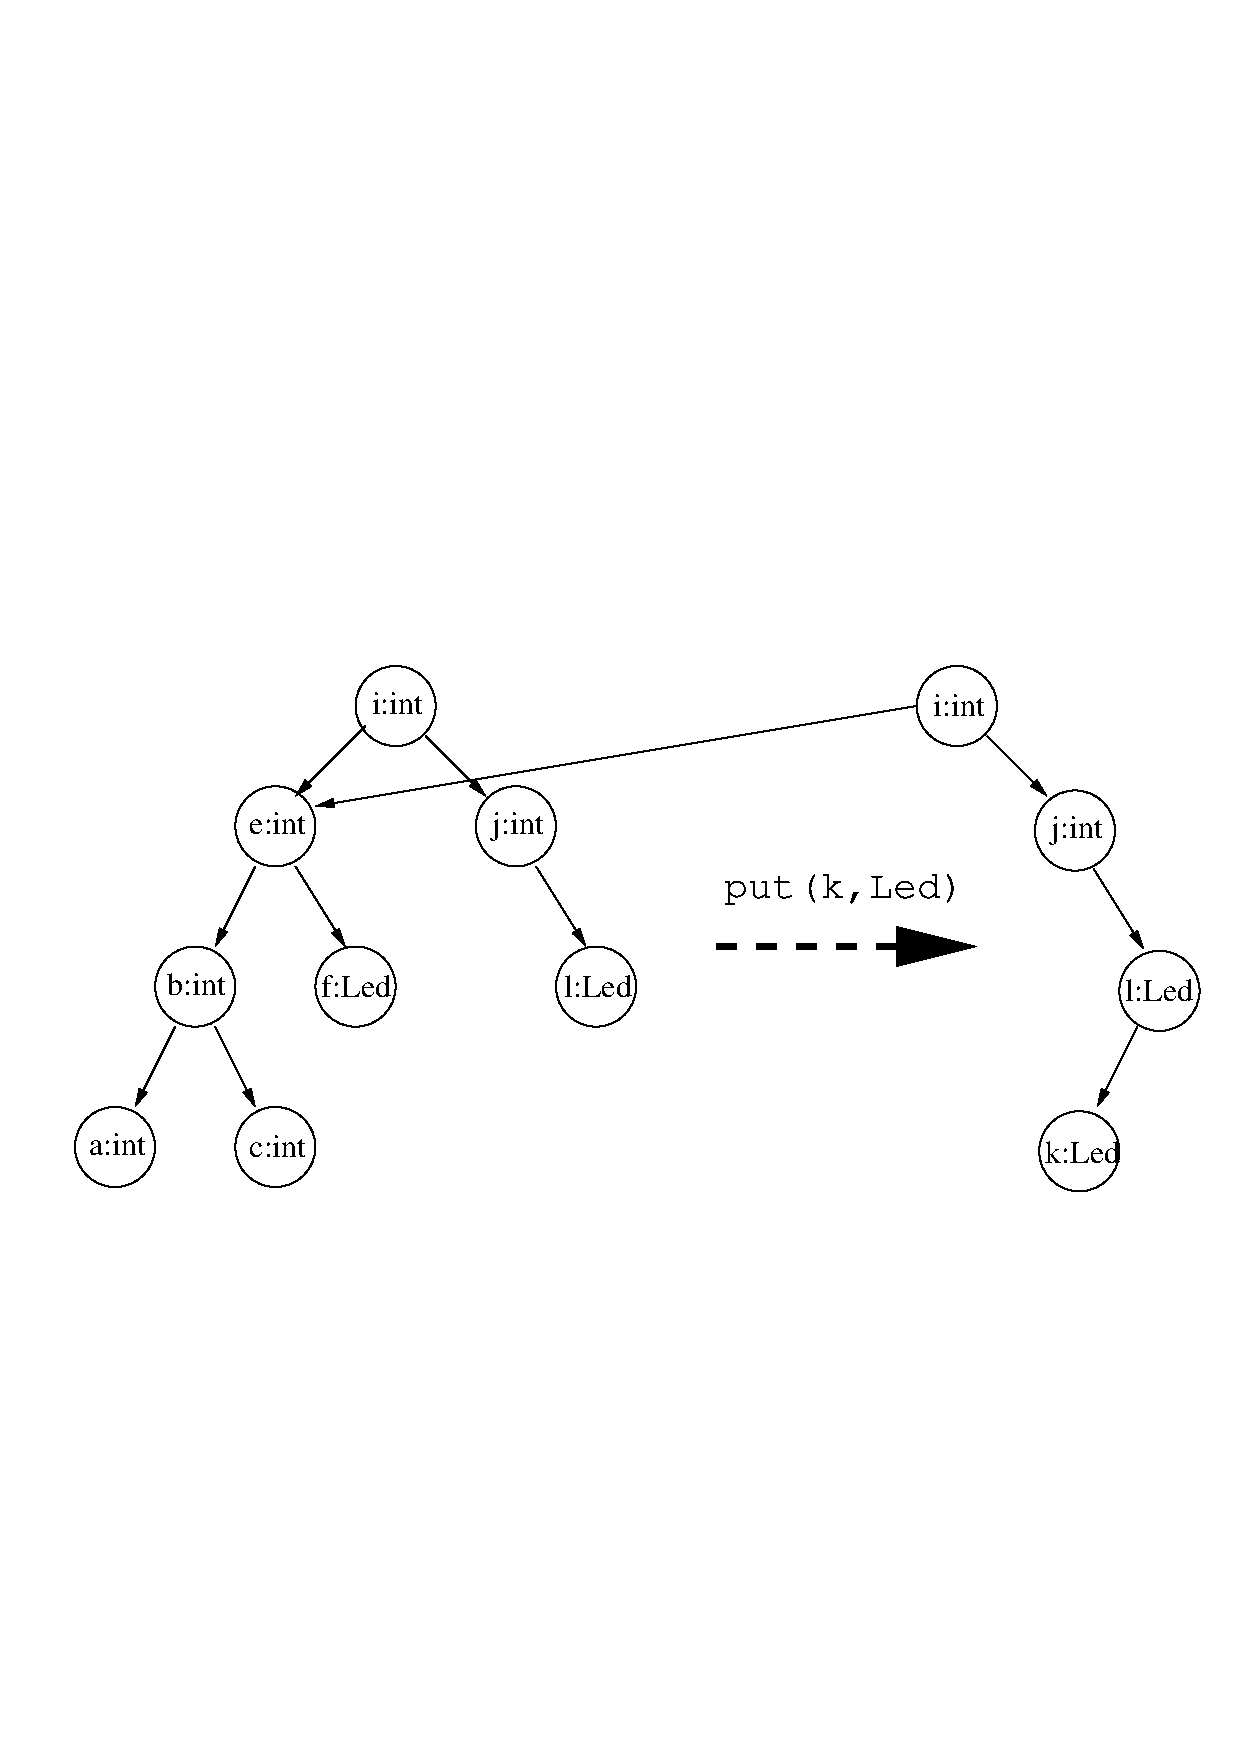
\includegraphics[width=15cm]{insertion.pdf}
\end{center}
\vspace*{-33ex}
\caption{L'inserzione non distruttiva di un legame per una variabile in un ambiente.}\label{fig:non_destructive}
\end{figure}

\begin{figure}[t]
{\small
\begin{verbatim}
       public class TypeChecker {
         private final Table<Type> env;
         private final ErrorMsg errorMsg;

         private TypeChecker(Table<Type> env, ErrorMsg errorMsg) {
           this.env = env; this.errorMsg = errorMsg;
         }
         public TypeChecker(ErrorMsg errorMsg) {
           this(Table.EMPTY, errorMsg);
         }
         public TypeChecker putVar(String var, Type type) {
           return new TypeChecker(env.put(var, type), errorMsg));
         }
         public Type getVar(String var) { return env.get(var); }
         public void error(int pos, String msg) { errorMsg.error(pos, msg); }
       }
\end{verbatim}
}
\caption{Il type-checker usato per effettuare l'analisi semantica delle espressioni Kitten.}
  \label{fig:semantical.TypeChecker1}
\end{figure}
%
Gli ambienti sono contenuti dentro un \emph{type-checker}, il quale
\e implementato dalla classe \texttt{semantical/TypeChecker.java}
in Figura~\ref{fig:semantical.TypeChecker1}.
Per adesso l'ambiente \`e tutto quello di cui abbiamo bisogno per
effettuare l'analisi semantica delle espressioni,
ma per i comandi aggiungeremo al type-checker ulteriori informazioni
(Sezione~\ref{sec:analysis_commands}).

Possiamo a questo punto implementare le regole
delle Figure~\ref{fig:analysis_expressions1} e~\ref{fig:analysis_expressions2}
tramite una discesa ricorsiva sulla sintassi astratta delle espressioni. In
\texttt{absyn/Expression.java} aggiungiamo:
%
\begin{verbatim}
  private Type staticType;
  private TypeChecker checker;

  public final Type typeCheck(TypeChecker checker) {
    return staticType = typeCheckAux(this.checker = checker);
  }

  protected abstract Type typeCheckAux(TypeChecker checker);
\end{verbatim}
%
Il metodo \texttt{public} e \texttt{final}, di nome \texttt{typeCheck()},
effettua le operazioni comuni a tutte le espressioni, \cioe
l'annotazione del tipo statico inferito per l'espressione e del type-checker
usato per inferirlo. Un metodo ausiliario e \texttt{protected}, di nome
\texttt{typeCheckAux()}, implementa le operazioni specifiche alla singola
espressione, come specificate nelle Figure~\ref{fig:analysis_expressions1}
e~\ref{fig:analysis_expressions2}.

Vediamo alcuni esempi di implementazione del metodo \texttt{typeCheckAux()}.
Dentro la classe \texttt{absyn/Variable.java} definiamo:
%
\begin{verbatim}
  protected Type typeCheckAux(TypeChecker checker) {
    Type result = checker.getVar(name);
    if (result == null) return error("undefined variable " + name);
    else return result;
  }
\end{verbatim}
%
Questa implementazione riflette la specifica in
Figura~\ref{fig:analysis_expressions1}: si cerca la variabile
nell'ambiente e se ne restituisce il tipo; se la variabile non
esiste nell'ambiente, si d\`a un errore.
Il metodo \texttt{error()} \e definito dentro
\texttt{absyn/Expression.java} come
%
\begin{verbatim}
  protected Type error(String msg) {
    error(checker, msg);
    return IntType.INSTANCE;
  }
\end{verbatim}
%
Esso stampa il messaggio di errore tramite il type-checker
in utilizzo per l'espressione e ritorna il tipo di emergenza \texttt{int}.
Questo permette di continuare il type-checking anche in presenza di un
errore, bench\'e possa causare degli errori di tipo a cascata.
Il metodo \texttt{error()} a due argomenti \e poi definito dentro
\texttt{absyn/Absyn.java} come
%
\begin{verbatim}
  protected void error(TypeChecker checker, String msg) {
    checker.error(pos, msg);
  }
\end{verbatim}
%
Esso usa il campo \texttt{pos} della sintassi astratta per indicare in che
punto dare l'errore all'utente. Tale campo era il numero di caratteri
tra l'inizio del file e un punto significativo della parte di sintassi
astratta in considerazione (Sezione~\ref{sec:abstract_syntax_classes}).

Esaminiamo un altro esempio, quello di \texttt{absyn/FieldAccess.java}:
%
\begin{verbatim}
  protected Type typeCheckAux(TypeChecker checker) {
    Type receiverType = receiver.typeCheck(checker);
    if (!(receiverType instanceof ClassType))
      return error("class type required");
    ClassType receiverClass = (ClassType) receiverType;
    if ((field = receiverClass.fieldLookup(name)) == null)
      return error("unknown field " + name);
    return field.getType();
  }
\end{verbatim}
%
Consistentemente con la Figura~\ref{fig:analysis_expressions1},
tale metodo effettua ricorsivamente l'analisi semantica di
\texttt{receiver} e quindi impone che esso abbia un tipo classe.
Infine cerca il campo di nome \texttt{name} dentro tale tipo classe
e ne restituisce il tipo.

Un altro esempio \e quello di \texttt{absyn/ArrayAccess.java}:
%
\begin{verbatim}
  protected Type typeCheckAux(TypeChecker checker) {
    Type arrayType = array.typeCheck(checker);
    index.mustBeInt(checker);
    if (!(arrayType instanceof ArrayType))
      return error("array type required");
    return ((ArrayType) arrayType).getElementsType();
  }
\end{verbatim}
%
Consistentemente con la Figura~\ref{fig:analysis_expressions1},
tale metodo effettua ricorsivamente l'analisi semantica di
\texttt{array} e \texttt{index}. Per \texttt{index} usa il metodo ausiliario
\texttt{mustBeInt()} che \e definito dentro \texttt{absyn/Expression.java}
come:
%
\begin{verbatim}
  protected void mustBeInt(TypeChecker checker) {
    if (typeCheck(checker) != IntType.INSTANCE) error("integer expected");
  }
\end{verbatim}

Consideriamo infine la definizione di \texttt{typeCheckAux()}
in \texttt{absyn/ArithmeticBinOp.java}:
%
\begin{verbatim}
  protected Type typeCheckAux(TypeChecker checker) {
    Type leftType = getLeft().typeCheck(checker);
    Type rightType = getRight().typeCheck(checker);
    if (leftType.canBeAssignedTo(FloatType.INSTANCE) &&
        rightType.canBeAssignedTo(FloatType.INSTANCE))
      return leftType.leastCommonSupertype(rightType);
    else return error("numerical argument required");
  }
\end{verbatim}
%
Consistentemente con la Figura~\ref{fig:analysis_expressions2},
esso effettua ricorsivamente l'analisi semantica di
\texttt{left} e \texttt{right} e impone che tali sottoespressioni
abbiano un tipo statico
che sia \texttt{float} o un sottotipo di \texttt{float}. Il tipo statico
dell'operazione binaria \e il minimo supertipo comune fra i tipi
statici di \texttt{left} e \texttt{right}.
%
\begin{figure}[t]
\begin{center}
{\small
  \[
    \frac{}
         {\rho\vdash\mathtt{Skip()}:\rho}\qquad
    \frac{\rho\vdash\mathit{condition}:\mathtt{BooleanType.INSTANCE}\quad
          \rho\vdash\mathit{then}:\rho'\quad
          \rho\vdash\mathit{else}:\rho''}
         {\rho\vdash\mathtt{IfThenElse(\mathit{condition},\mathit{then},
          \mathit{else}):\rho}}
  \]
  \[
    \frac{\mathit{expression}\not=\mathtt{null}\quad
          \rho\vdash\mathit{expression}:t\quad
          \text{il comando occorre in un metodo che ritorna $r$}
          \quad t\le r}
         {\rho\vdash\mathtt{Return(\mathit{expression})}:\rho}
  \]
  \[
    \frac{\text{il comando occorre in un costruttore o in un metodo che
                ritorna \texttt{void}}}
         {\rho\vdash\mathtt{Return(null)}:\rho}
  \]
  \[
    \frac{\rho\vdash\mathit{lvalue}:t_l\quad\rho\vdash\mathit{rvalue}:t_r
          \quad t_r\le t_l}
         {\rho\vdash\mathtt{Assignment(\mathit{lvalue},\mathit{rvalue})}:\rho}
  \]
  \[
    \frac{\rho\vdash\mathit{initialisation}:\rho'\quad
          \rho'\vdash\mathit{condition}:\mathtt{BooleanType.INSTANCE}\quad
          \rho'\vdash\mathit{update}:\rho''\quad
          \rho'\vdash\mathit{body}:\rho'''}
         {\rho\vdash\mathtt{For(\mathit{initialisation},\mathit{condition},
          \mathit{update},\mathit{body})}:\rho}
  \]
  \[
    \frac{\rho\vdash\mathit{condition}:\mathtt{BooleanType.INSTANCE}\quad
          \rho\vdash\mathit{body}:\rho'}
         {\rho\vdash\mathtt{While(\mathit{condition},\mathit{body})}:\rho}
  \]
  \[
    \frac{t=\st{\mathit{type}}\quad\rho\vdash\mathit{initialiser}:i\quad 
          i\le t}
         {\rho\vdash\mathtt{LocalDeclaration(\mathit{type},\mathit{name},
          \mathit{initialiser})}:\rho[\mathit{name}\mapsto t]}
  \]
  \[
    \frac{\rho\vdash\mathit{body}:\rho'}
         {\rho\vdash\mathtt{LocalScope(\mathit{body})}:\rho}
    \qquad
     \frac{\begin{array}{c}
       \rho\vdash\mathit{receiver}:\kappa\quad\kappa\in\mathtt{ClassType}
         \quad\rho\vdash\mathit{actuals}:\vec{\tau}\\
       \kappa\mathtt{.methodsLookup(\mathit{name},}\vec{\tau})=
           \{\mathit{method}\}
       \end{array}}
          {\rho\vdash\mathtt{MethodCallCommand(\mathit{receiver},
           \mathit{name},\mathit{actuals})}:\rho}
  \]
  \[
    \frac{\rho\vdash c_1:\rho'\quad\rho'\vdash c_2:\rho''}
         {\rho\vdash c_1;c_2:\rho''}
  \]
}
\end{center}
\caption{Le regole per l'analisi semantica dei comandi Kitten.}
  \label{fig:analysis_commands}
\end{figure}
%
\section{L'analisi semantica dei comandi Kitten}
  \label{sec:analysis_commands}
%
La Figura~\ref{fig:analysis_commands} mostra le regole di analisi semantica
per i comandi Kitten. Questa volta usiamo un giudizio
$\rho\vdash c:\rho'$ il cui significato \e che il comando $c$
eseguito a partire da un ambiente $\rho$ porta in un ambiente $\rho'$.
Questo perch\'e i comandi non hanno un valore ma possono modificare l'ambiente
e le uniche modifiche visibili al livello dei tipi sono quelle dell'insieme
e del tipo delle variabili in scope. In particolare, \e la dichiarazione di una
variabile (la \texttt{LocalDeclaration} in Figura~\ref{fig:analysis_commands})
che estende l'ambiente con una nuova variabile locale, che sostituisce
eventualmente una variabile gi\`a in scope e con lo stesso nome.

Esaminiamo adesso alcune regole della Figura~\ref{fig:analysis_commands}:
%
\begin{description}
\item[\underline{$\mathtt{IfThenElse(\mathit{condition},\mathit{then},\mathit{else})}$}.]
  Il condizionale richiede che la condizione sia un'espressione di tipo
  booleano ed effettua ricorsivamente
  l'analisi semantica di $\mathit{then}$ ed $\mathit{else}$.
  La scelta di lasciare $\rho$ immutato come risultato
  dell'analisi semantica del condizionale implica che eventuali variabili
  locali dichiarate all'interno del ramo \textit{then} o del
  ramo \textit{else} (o di entrambe)
  non sono \piu in scope alla fine del condizionale.
\item[\underline{$\mathtt{Return(\mathit{expression})}$}.]
  Il comando di ritorno da metodo o costruttore richiede di effettuare
  ricorsivamente l'analisi semantica dell'espressione ritornata, se esiste.
  Nel caso in cui essa non sia \texttt{null}, allora questo comando deve
  trovarsi dentro un metodo che ritorna il tipo statico
  di $\mathit{expression}$ o un suo supertipo. Altrimenti questo comando
  deve trovarsi dentro un metodo che ritorna \texttt{void} o dentro
  un costruttore.
\item[\underline{$\mathtt{Assignment(\mathit{lvalue},\mathit{rvalue})}$}.]
  L'analisi semantica dell'assegnamento del valore di un'espressione
  a un leftvalue consiste nel controllare che il tipo statico dell'espressione
  sia lo stesso o un sottotipo del tipo statico del leftvalue.
\item[\underline{$\mathtt{For(\mathit{initialisation},\mathit{condition},
  \mathit{update},\mathit{body})}$}.]
  L'analisi semantica del ciclo \texttt{for} comincia analizzando
  ricorsivamente il comando \textit{initialisation}. Il risultato di questa
  analisi \`e un ambiente $\rho'$, eventualmente arricchito, rispetto a
  $\rho$, con una dichiarazione di una variabile locale al ciclo.
  Si impone poi che \textit{condition} abbia tipo booleano. L'ambiente $\rho'$
  viene usato per effettuare l'analisi
  semantica di \textit{initialisation}, \textit{update} e \textit{body},
  al fine di permettere al programmatore di dichiarare una variabile locale
  dentro \textit{initialisation} e di usarla nelle altre componenti del
  \texttt{for}, come in
  \begin{verbatim}
    for (int i := 0; i < 5; i := i + 1) "".concat(i).output()
  \end{verbatim}
  \vspace*{-2.5ex}
  Se si fosse usato $\rho$ per l'analisi di \emph{condition}, \emph{update} e
  \emph{body},
  la variabile \texttt{i} sarebbe risultata indefinita o avrebbe fatto
  riferimento a un'altra variabile, definita esternamente al ciclo.
\item[\underline{$\mathtt{LocalDeclaration(\mathit{type},\mathit{name},\mathit{initialiser})}$}.]
  L'analisi semantica della dichiarazione di una variabile locale estende
  l'ambiente legando la variabile \textit{name} al tipo semantico di
  \textit{type}. Ricorsivamente si effettua anche
  l'analisi semantica di \textit{initialiser} e si impone che il suo tipo
  statico sia lo stesso o un sottotipo del tipo semantico di \textit{type}.
\item[\underline{$\mathtt{LocalScope(\mathit{body})}$}.]
  L'analisi semantica della creazione di uno scope locale effettua
  ricorsivamente l'analisi semantica del corpo dello scope. Definendo
  $\rho$ come risultato di questa analisi semantica, facciamo in modo che
  eventuali variabili locali dichiarate all'interno del corpo
  non siano \piu visibili all'esterno dello scope. Per esempio, nel comando
  \verb!{ int a; a := 5 }! la variabile
  \texttt{a} non \e \piu visibile dopo la parentesi graffa di chiusura.
\item[\underline{$\mathtt{MethodCallCommand(\mathit{receiver},\mathit{name},\mathit{actuals})}$}.]
  L'analisi semantica del comando di invocazione di metodo \e
  estremamente simile a quella dell'espressioni di invocazione di metodo
  in Figura~\ref{fig:analysis_expressions2}. L'unica differenza \e che qui
  non imponiamo alcun vincolo sul tipo di ritorno del metodo, che pu\`o
  quindi anche essere \texttt{void}.
\item[\underline{$c_1;c_2$}.]
  L'analisi semantica della sequenza di comandi si richiama ricorsivamente
  sui due comandi, usando l'ambiente risultante dall'analisi semantica del
  primo per effettuare l'analisi semantica del secondo. In questo modo
  eventuali variabili locali dichiarate in $c_1$ possono essere usate da $c_2$.
\end{description}
%
\subsection{L'implementazione dell'analisi semantica dei comandi}
  \label{subsec:analysis_commands_implementation}
%
Dal momento che l'analisi semantica di un comando restituisce un ambiente, implementiamo
il metodo di analisi semantica dentro \texttt{absyn/Command.java} come
%
\begin{verbatim}
  private TypeChecker checker;

  public final TypeChecker typeCheck(TypeChecker checker) {
    return checker = typeCheckAux(this.checker = checker);
  }

  protected abstract TypeChecker typeCheckAux(TypeChecker checker);
\end{verbatim}
%
Il metodo \texttt{public} e \texttt{final} di nome \texttt{typeCheck()}
effettua la parte di analisi semantica comune a tutti i comandi, che consiste
nel chiamare il metodo ausiliario \texttt{typeCheckAux()} e prendere nota del
type-checker risultante dall'analisi.

Il metodo \texttt{typeCheckAux()} effettua la parte di analisi semantica
specifica a ciascun comando, secondo le regole della
Figura~\ref{fig:analysis_commands}. Per esempio, dentro
\texttt{absyn/IfThenElse.java} lo definiamo come
%
\begin{verbatim}
  protected TypeChecker typeCheckAux(TypeChecker checker) {
    condition.mustBeBoolean(checker);
    then.typeCheck(checker);
    else.typeCheck(checker);
    return checker;
  }
\end{verbatim}
%
Invece dentro \texttt{absyn/For.java} lo definiamo come
%
\begin{verbatim}
  protected TypeChecker typeCheck$0(TypeChecker checker) {
    TypeChecker initChecker = initialisation.typeCheck(checker);
    condition.mustBeBoolean(initChecker);
    update.typeCheck(initChecker);
    body.typeCheck(initChecker);
    return checker;
  }
\end{verbatim}
%
\begin{figure}[t]
{\small
\begin{verbatim}
public class TypeChecker {
  private final Type returnType;
  private final Table<TypeAndNumber> env;   
  private final int varNum;
  private final ErrorMsg errorMsg;

  private TypeChecker(Type returnType, Table<TypeAndNumber> env,
      int varNum, ErrorMsg errorMsg) {
    this.returnType = returnType; this.env = env;
    this.varNum = varNum; this.errorMsg = errorMsg;
  }
  public TypeChecker(Type returnType, ErrorMsg errorMsg) {
    this(returnType, Table.EMPTY, 0, errorMsg);
  }
  public Type getReturnType() { return returnType; }
  public TypeChecker putVar(String var, Type type) {
    return new TypeChecker
      (returnType, env.put(var, new TypeAndNumber(type, varNum)), varNum + 1, errorMsg);
  }
  public Type getVar(String var) {
    TypeAndNumber tan = env.get(var);
    if (tan != null) return tan.getType(); else return null;
  }
  public int getVarNum(String var) {
    TypeAndNumber tan = env.get(var);
    if (tan != null) return tan.getNumber(); else return -1;
  }
}
\end{verbatim}
}
\caption{Una versione potenziata della classe \texttt{semantical/TypeChecker.java} che implementa un type-checker.}
  \label{fig:semantical.TypeChecker}
\end{figure}
%
Si noti in quest'ultimo esempio come l'ambiente (in effetti, il type-checker)
risultante dall'analisi di \texttt{initialisation} sia poi usato per effettuare
l'analisi semantica di \texttt{condition}, \texttt{update} e \texttt{body}, ma
come poi venga ritornato il type-checker di partenza, senza l'eventuale
legame per le variabili dichiarate nell'espressione di inizializzazione,
conformemente alla Figura~\ref{fig:analysis_commands}.

La Figura~\ref{fig:semantical.TypeChecker} mostra una revisione del
type-checker della Figura~\ref{fig:semantical.TypeChecker1}.
Adesso esso conosce il tipo di ritorno del metodo che
si sta analizzando, fornito al momento della
costruzione del type-checker tramite l'unico costruttore pubblico
in Figura~\ref{fig:semantical.TypeChecker} e usato poi per
implementare l'analisi semantica dei comandi \texttt{return}: in
\texttt{absyn/Return.java} definiamo infatti:
%
\begin{verbatim}
  protected TypeChecker typeCheckAux(TypeChecker checker) {
    Type expectedReturnType = checker.getReturnType();
    if (returned == null && expectedReturnType != VoidType.INSTANCE)
      error("missing return value");
    if (returned != null &&
        !returned.typeCheck(checker).canBeAssignedTo(expectedReturnType))
      error("illegal return type: " + expectedReturnType + " expected");
    return checker;
  }
\end{verbatim}
% $
conformemente alla Figura~\ref{fig:analysis_commands}.

Si noti che il type-checker potenziato come
in Figura~\ref{fig:semantical.TypeChecker} associa adesso
alle variabile dell'ambiente non solo il loro tipo di dichiarazione,
ma anche un numero progressivo che indica la quantit\`a di variabili
viste finora in un metodo, informazione che ci sar\`a utile in fase di generazione del
codice (Capitolo~\ref{chap:translate}).
%
\section{L'analisi semantica delle classi Kitten}
  \label{sec:analysis_classes}
%
Fare l'analisi semantica di una classe Kitten significa effettuare
l'analisi semantica dei suoi membri, \cioe campi, costruttori e metodi.
Nulla va controllato per quanto riguarda i campi. Per quanto riguarda
costruttori e metodi, invece, occorre effettuare l'analisi semantica
del loro corpo. Essendo il loro corpo un comando, possiamo usare a tal
fine le regole della Figura~\ref{fig:analysis_commands}, cominciando
l'analisi da un ambiente iniziale in cui i parametri del costruttore o del
metodo sono legati al loro tipo di dichiarazione (incluso il parametro
implicito \texttt{this}). A tal fine, definiamo una funzione che
aggiunge a un ambiente una lista di variabili dichiarate come parametri
formali:
%
\begin{align*}
  \rho+{\mathtt{null}}&=\rho \\
  \rho+{\mathtt{FormalParameters(\mathit{type},\mathit{name},\mathit{next})}}&=(\rho+{\mathit{next}})[\mathit{name}\mapsto\st{type}]
\end{align*}
%
L'analisi semantica di un costruttore o metodo con parametri formali
$\mathit{formals}$ e dichiarato in una classe
il cui tipo semantico \`e $\kappa$ viene quindi effettuata
a partire da un ambiente iniziale
\[
  \overline{\rho}=[\mathtt{this}\mapsto\kappa]+{\mathit{formals}}
\]
Se $\mathit{body}$ \`e il corpo del costruttore o metodo, si tratter\`a
di verificare che il giudizio $\overline{\rho}:\mathit{body}:\rho'$ sia
valido per un qualche $\rho'$.

Anche il metodo che fa l'analisi semantica dei membri di una classe si
chiama \texttt{typeCheck()}. Esso \`e definito dentro
\texttt{absyn/ClassMemberDeclaration.java} come
%
\begin{verbatim}
  final void typeCheck(ClassType currentClass) {
    typeCheck$0(currentClass);
    if (next != null) next.typeCheck(currentClass);
  }

  protected abstract void typeCheck$0(ClassType currentClass);
\end{verbatim}
% $
ovvero tramite il solito metodo \texttt{final} che richiama, su tutta la
lista dei membri della classe, il metodo ausiliario
\texttt{typeCheck\$0()} che effettua l'analisi specifica a ciascun membro.
Abbiamo detto che l'analisi semantica dei campi non richiede nessun controllo:
dentro la classe di sintassi astratta
\texttt{absyn/FieldDeclaration.java} definiamo quindi:
%
\begin{verbatim}
  protected void typeCheck$0(ClassType currentClass) {}
\end{verbatim}
% $
In \texttt{absyn/ConstructorDeclaration.java} definiamo invece:
%
\begin{verbatim}
  protected void typeCheck$0(ClassType currentClass) {
    TypeChecker checker
      = new TypeChecker(VoidType.INSTANCE, currentClass.getErrorMsg());
    checker = checker.putVar(Symbol.THIS,currentClass);
    if (getFormals() != null) checker = getFormals().typeCheck(checker);
    getBody().typeCheck(checker);
    getBody().checkForDeadcode();
  }
\end{verbatim}
% $
Questo metodo comincia col costruire un type-checker con ambiente vuoto e
che si aspetta come tipo di ritorno \texttt{VoidType.INSTANCE}. Quindi aggiunge
la variabile \texttt{this} legata al tipo semantico
della classe e i parametri formali legati al loro tipo di dichiarazione,
rispecchiando la definizione precedente di $\overline{\rho}$.
Infine effettua il type-checking del corpo del costruttore e controlla che al
suo interno non ci sia del codice morto (Sezione~\ref{sec:dead_code}).
Il ragionamento \e simile nel caso della dichiarazione di un metodo,
ma si usa il tipo di ritorno del metodo al posto di \texttt{VoidType.INSTANCE} e si
controlla che se il metodo ne ridefinisce un
altro di una superclasse allora la ridefinizione del tipo di ritorno
soddisfi il test \texttt{canBeAssignedToSpecial()}
visto in Sezione~\ref{sec:semantical_types}. Se inoltre il metodo non
ritorna \texttt{void}, si impone che il valore di ritorno del metodo
\texttt{checkForDeadcode()} sia \texttt{true}, in modo da garantire che
il metodo termini sempre con un comando \texttt{return}.

\greycomment{
L'analisi semantica di Kitten descritta in questo capitolo \e un po'
semplificata rispetto alla realt\`a. In particolare non abbiamo considerato
come dall'analisi della classe di partenza
(Sezione~\ref{sec:analysis_classes}) si arrivi a quella
delle altre classi a cui essa fa riferimento. Questo \e ottenuto
facendo in modo che le regole delle Figure~\ref{fig:analysis_expressions1},
\ref{fig:analysis_expressions2} e~\ref{fig:analysis_commands}, quando
hanno bisogno di ottenere il tipo semantico delle espressioni di tipo,
richiamino ricorsivamente il type-checking su tutte le classi che vi occorrono.
Al fine di evitare cicli, si usa un flag
\texttt{typeChecked} all'interno di \texttt{types.ClassType}.}
%
\begin{exercise}\label{ex:conditional_expression}
Si aggiunga alle espressioni la sintassi astratta di un'\emph{espressione
condizionale}
$\mathit{exp}_1\mathtt{?}\,\mathit{exp}_2\,\mathtt{:}\,\mathit{exp}_3$
che restituisce il valore di $\mathit{exp}_2$ se $\mathit{exp}_1$ \e
vera e il valore di $\mathit{exp}_3$ altrimenti. Si dia la sua regola di
type-checking.
\end{exercise}
%
\begin{exercise}\label{ex:switch}
Si aggiunga ai comandi la sintassi astratta di un comando \texttt{switch}.
Non ci si limiti a espressioni costanti nei vari casi.
Si dia la regola di type-checking per tale comando.
\end{exercise}
%
\begin{exercise}\label{ex:break_continue}
Si aggiunga ai comandi la sintassi astratta dei comandi
\texttt{break} e \texttt{continue}. Si diano le loro regole di type-checking,
che devono garantire che tali comandi occorrano solo dentro un ciclo.
Come modifichereste il type-checker in Figura~\ref{fig:semantical.TypeChecker}
in modo da implementare tali controlli?
\end{exercise}

\chapter{Generazione del Bytecode Kitten}\label{chap:translate}
%
\vspace*{-2ex}
\begin{center}

\includegraphics[width=6.5cm]{cat9.jpg}
\end{center}
%\vspace*{-2ex}
%
L'analisi semantica del Capitolo~\ref{chap:semantical} ha garantito che
il codice Kitten non contenga alcun errore semantico. Ha inoltre
annotato l'albero di sintassi astratta con informazioni relative
al tipo statico delle espressioni che vi occorrono; gli accessi a
campi, costruttori e metodi con la specifica dichiarazione
del campo, costruttore
o metodo a cui fanno riferimento. Siamo ora nelle condizioni di
generare del codice \emph{intermedio}, \cioe indipendente dall'architettura
verso la quale stiamo compilando, ma pensato piuttosto per essere
facilmente sintetizzabile a partire dall'albero di sintassi astratta
e facilmente ottimizzabile. Esso verr\`a poi traslato in codice oggetto,
specifico all'architettura verso cui compiliamo.
Il codice intermedio che useremo \`e il \emph{bytecode Kitten}, che pu\`o
essere visto come una versione semplificata ed esplicitamente tipata del
\emph{Java bytecode}.
%
\section{Il bytecode Kitten}
%
Il bytecode Kitten \`e un linguaggio di programmazione pensato per
essere eseguito da una macchina astratta che ha a disposizione:
%
\begin{enumerate}
\item un insieme di \emph{variabili locali}, potenzialmente illimitato, che
      possono contenere valori primitivi o riferimenti a oggetti o array;
\item uno stack di variabili temporanee, detto \emph{stack degli operandi},
      potenzialmente illimitato, che pu\`o contenere valori primitivi o
      riferimenti a oggetti o array;
\item uno \emph{stack di attivazione}, formato da un numero potenzialmente
      illimitato di \emph{frame di attivazione} di metodi. Ciascun frame
      di attivazione contiene le variabili locali e lo stack di attivazione
      di un metodo;
\item una \emph{memoria} o \emph{heap}, che contiene oggetti e array
      allocati dinamicamente dal programma in esecuzione.
\end{enumerate}

La maggior parte delle istruzioni del bytecode Kitten operano sulle
variabili locali e sullo stack degli operandi. Un numero limitato
(invocazione e ritorno da metodo) operano anche sullo stack di attivazione.
Le sole operazioni che operano sulla memoria sono quelle
di creazione di oggetto o array e di accesso a campi o array.
%
\begin{figure}[t]
\begin{verbatim}
      Led():                                    isOn():
        return void                               load 0 of type Led
                                                  getfield Led.state
      on():                                       return boolean
        load 0 of type Led
        const true                              isOff():
        putfield Led.state                        load 0 of type Led
        return void                               getfield Led.state
                                                  neg boolean
      off():                                      return boolean
        load 0 of type Led
        const false
        putfield Led.state
        return void
\end{verbatim}
\caption{La compilazione in bytecode Kitten dei metodi della classe \texttt{Led} in Figura~\ref{fig:led}.}\label{fig:led_bytecode}
\end{figure}

Si consideri la Figura~\ref{fig:led_bytecode}. Essa mostra la compilazione
in bytecode Kitten dei metodi della classe \texttt{Led} in
Figura~\ref{fig:led}. All'inizio dell'esecuzione di un metodo o costruttore,
lo stack degli operandi \`e vuoto e le variabili locali contengono i
parametri attuali del metodo o costruttore. In particolare, la variabile
locale numero $0$ contiene sempre il riferimento all'oggetto corrente,
\cioe quello che nel codice sorgente sarebbe stato \texttt{this}, che \e
un parametro implicito in tutte le chiamate di metodo o costruttore. La
variabile locale $1$ contiene il primo parametro attuale esplicito,
la variabile locale $2$ il secondo parametro attuale esplicito, e \cosi via.
Si noti comunque che le variabili locali possono essere usate anche per
contenere vere e proprie variabili locali ai metodi e non solo per contenere
i parametri attuali. Nell'esempio
in Figura~\ref{fig:led_bytecode}, solo la variabile locale $0$ \`e utilizzata,
dal momento che nessun metodo richiede dei parametri espliciti \nec
variabili locali.
L'istruzione \texttt{load 0 of type Led}
indica di copiare il riferimento all'oggetto corrente in cima allo
stack degli operandi. L'istruzione \texttt{const} serve invece a caricare
in cima allo stack degli operandi una costante. Nella
Figura~\ref{fig:led_bytecode} si tratta di una costante booleana.
Le istruzioni \texttt{getfield} e \texttt{putfield} servono, rispettivamente,
a leggere e a scrivere un campo di un oggetto. L'istruzione \texttt{neg}
nega il valore che sta in cima allo stack degli operandi. L'istruzione
\texttt{return} termina l'esecuzione di un metodo o costruttore ritornando
possibilmente un valore al chiamante.

\begin{figure}[t]
\begin{center}
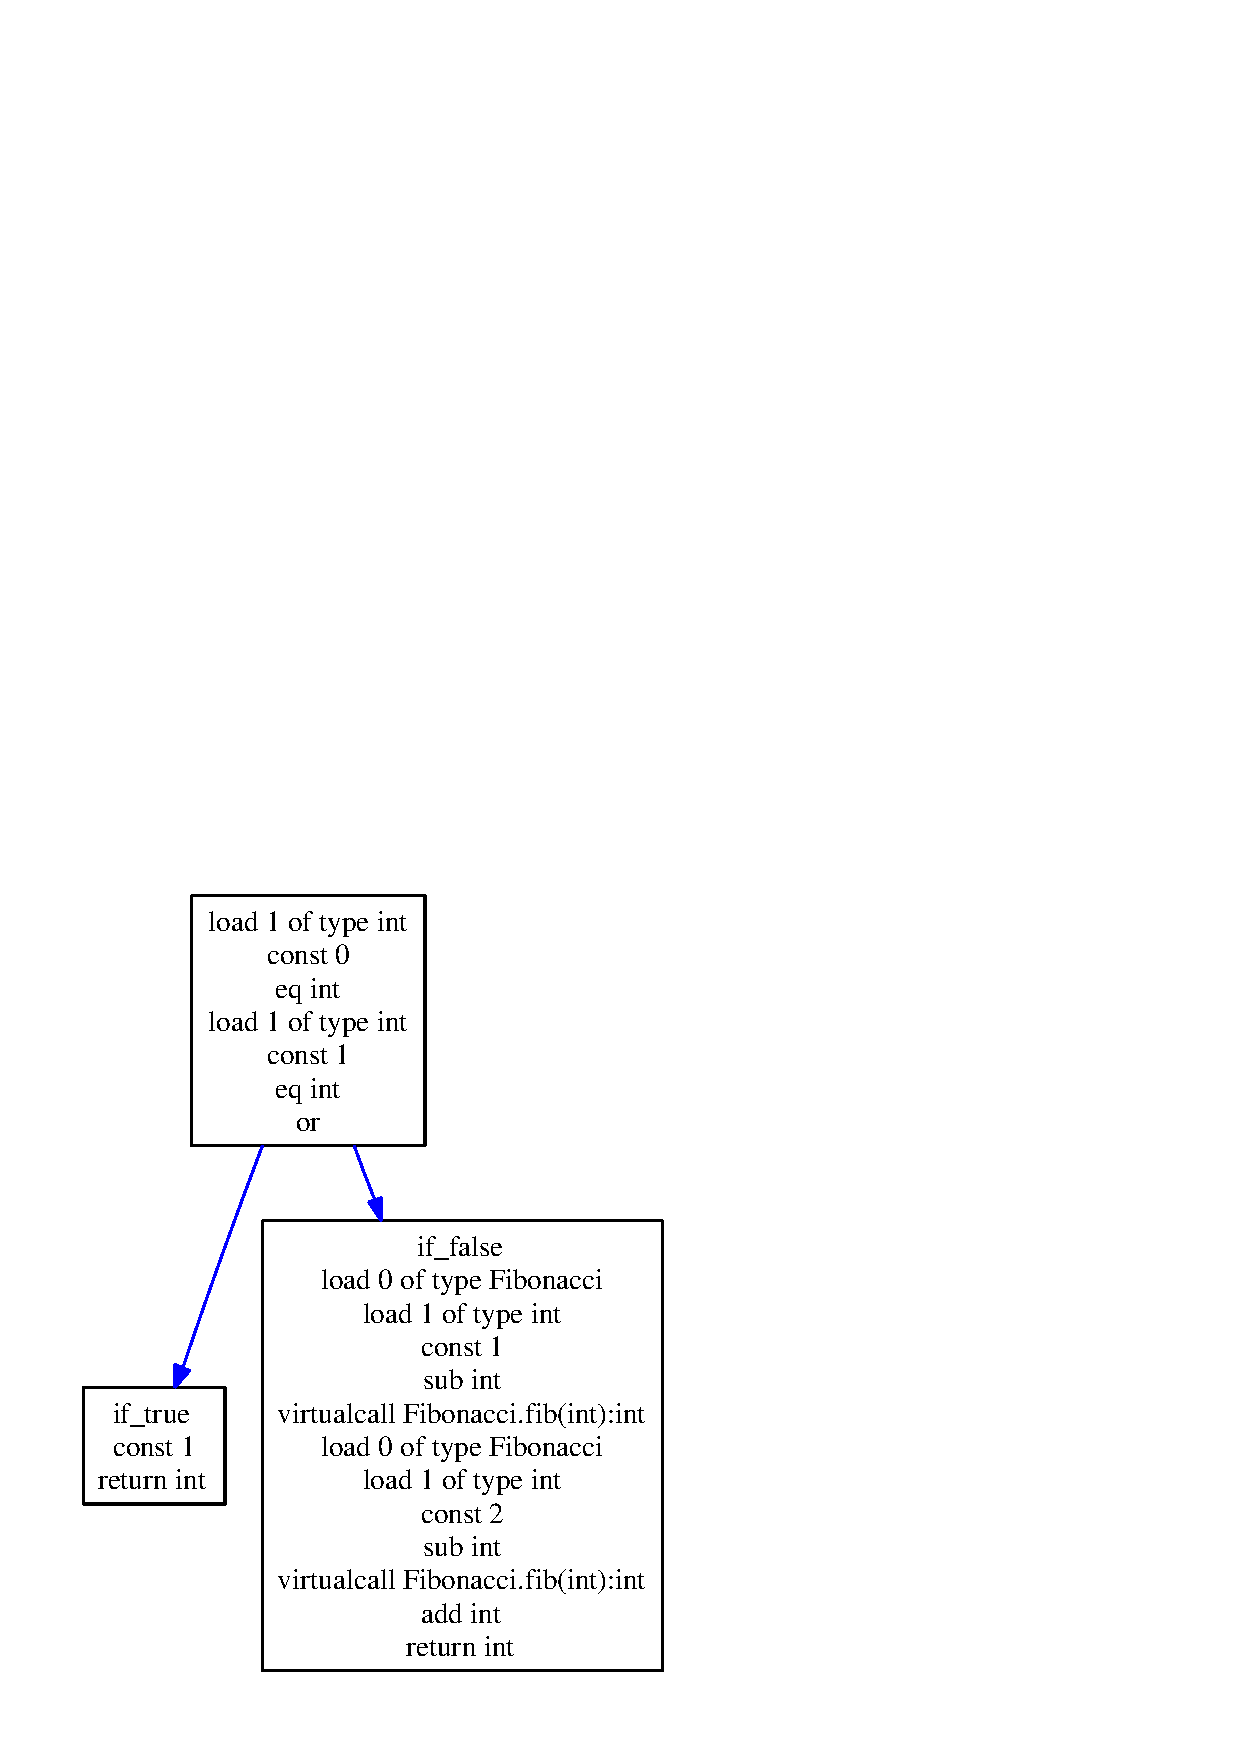
\epsfig{file = fib.pdf, width = 8cm}
\end{center}
\caption{La compilazione in bytecode Kitten del metodo \texttt{fib()} in Figura~\ref{fig:fibonacci}.}\label{fig:fib_bytecode}
\end{figure}
%
Il bytecode in Figura~\ref{fig:led_bytecode} ha una struttura di controllo
particolarmente semplice, dal momento che non prevede condizionali \nec cicli.
La Figura~\ref{fig:fib_bytecode} mostra un esempio \piu complesso:
la compilazione in bytecode Kitten del metodo \texttt{fib()} in
Figura~\ref{fig:fibonacci}. La presenza di un comando condizionale in
Figura~\ref{fig:fibonacci} diventa un'alternativa di controllo nel
bytecode Kitten in Figura~\ref{fig:fib_bytecode}: il risultato dell'istruzione
\texttt{or} determina l'istradamento del controllo verso il ramo
\texttt{if\_true} o verso quello \texttt{if\_false}.

L'esempio precedente mostra che il bytecode Kitten \`e in effetti un grafo
di \emph{blocchi di codice} che contengono codice
sequenziale. Un ulteriore esempio \`e la compilazione del ciclo:
%
\begin{verbatim}
  for (int i := 0; i < 5; i := i + 1) {}
\end{verbatim}
%
mostrata in Figura~\ref{fig:cycle_bytecode}. Questa volta
l'istradamento del controllo dipende dal risultato di un confronto.
In particolare, il confronto fra la variabile locale $1$, che contiene
la variabile \texttt{i} del ciclo, e la costante intera $5$ determina
l'istradamento del codice verso il ramo \texttt{if\_cmplt}
(\emph{IF the CoMParison is Less Than}) o verso quello
\texttt{if\_cmpge} (\emph{IF the CoMParison is Greater than or Equal}).
%
\begin{figure}[t]
\begin{center}
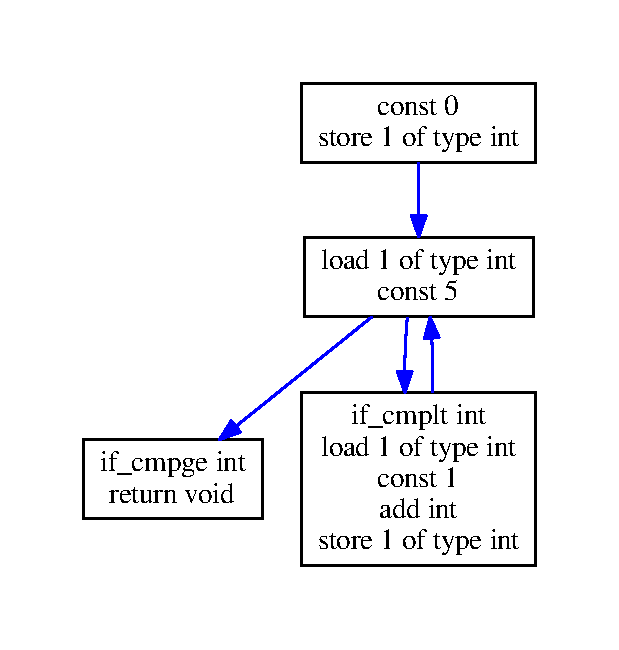
\epsfig{file = ciclo.pdf, width = 8cm}
\end{center}
\caption{La compilazione in bytecode Kitten di un ciclo \texttt{for}.}\label{fig:cycle_bytecode}
\end{figure}
%
\subsection{Le istruzioni sequenziali}\label{subsec:sequential_bytecodes}
%
\begin{figure}
\begin{center}
\begin{tabular}{|c|}
\hline\mbox{}\\
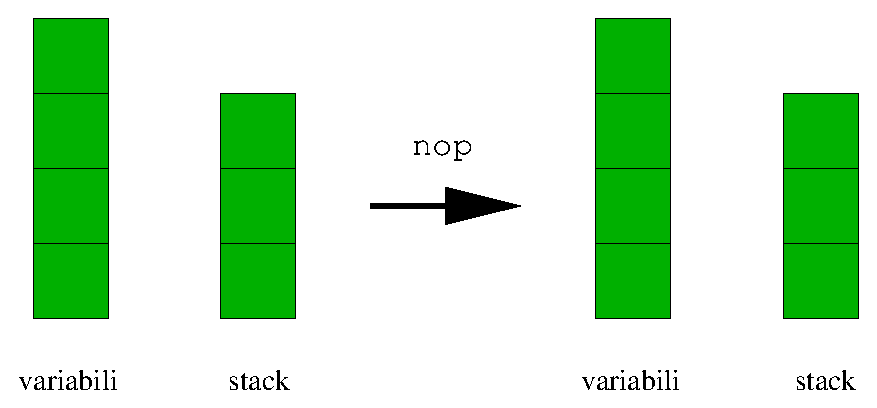
\epsfig{file = bytecodes/nop.eps, width = 12cm}\\\hline
\mbox{}\\
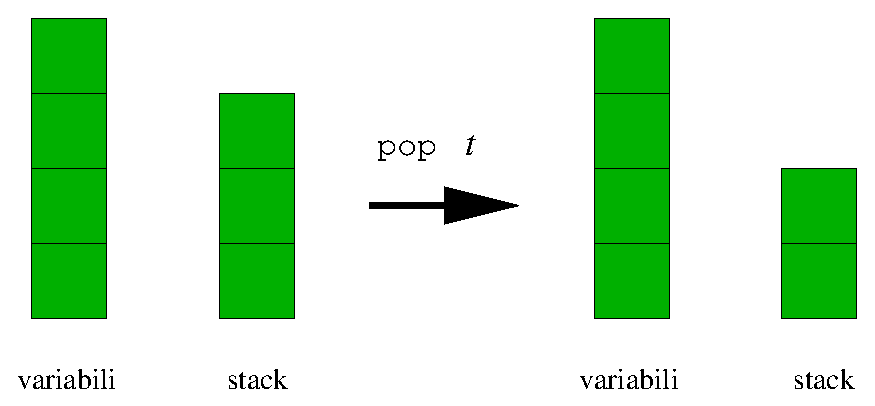
\epsfig{file = bytecodes/pop.eps, width = 12cm}\\\hline
\mbox{}\\
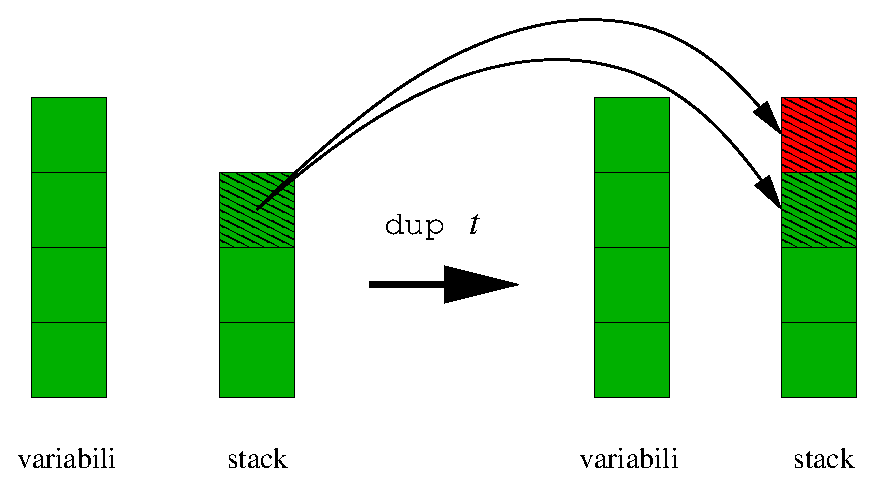
\epsfig{file = bytecodes/dup.eps, width = 12cm}\\\hline
\end{tabular}
\end{center}
\caption{Le istruzioni \texttt{nop}, \texttt{pop} e \texttt{dup} del bytecode Kitten.}
  \label{fig:bytecodes1}
\end{figure}
%
\begin{figure}
\begin{center}
\begin{tabular}{|c|}
\hline\mbox{}\\
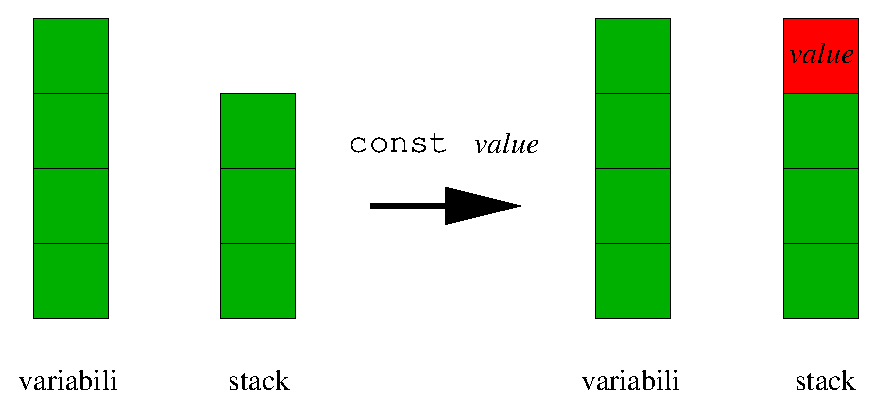
\epsfig{file = bytecodes/const.eps, width = 12cm}\\\hline
\hline\mbox{}\\
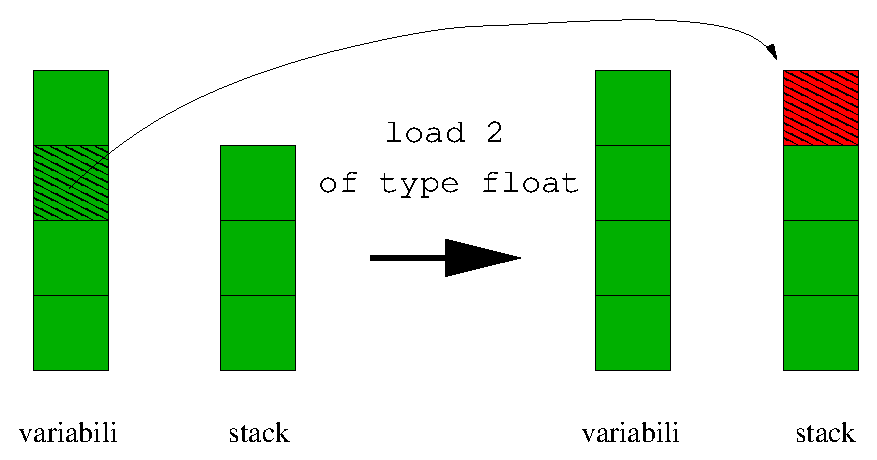
\epsfig{file = bytecodes/load.eps, width = 12cm}\\\hline
\mbox{}\\
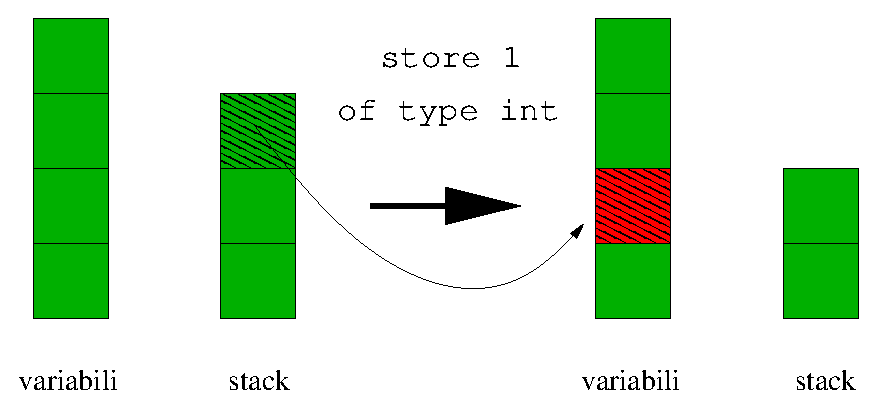
\epsfig{file = bytecodes/store.eps, width = 12cm}\\\hline
\end{tabular}
\end{center}
\caption{Le istruzioni \texttt{const}, \texttt{load} e \texttt{store} del bytecode Kitten.}
  \label{fig:bytecodes2}
\end{figure}
%
\begin{figure}
\begin{center}
\begin{tabular}{|c|}
\hline\mbox{}\\
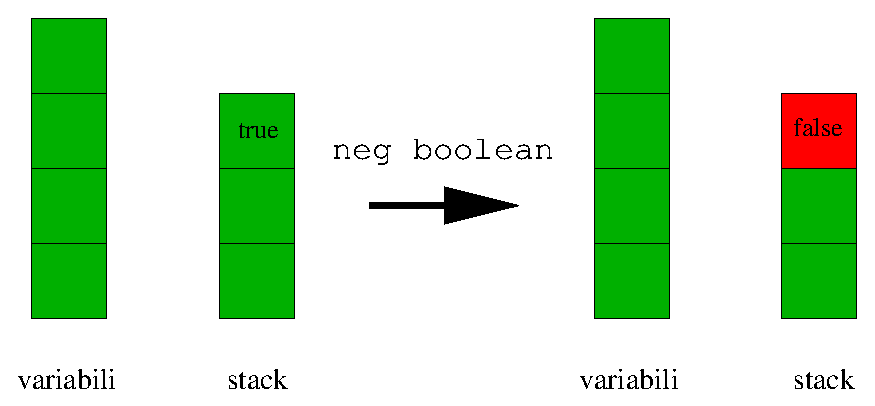
\epsfig{file = bytecodes/neg.eps, width = 12cm}\\\hline
\mbox{}\\
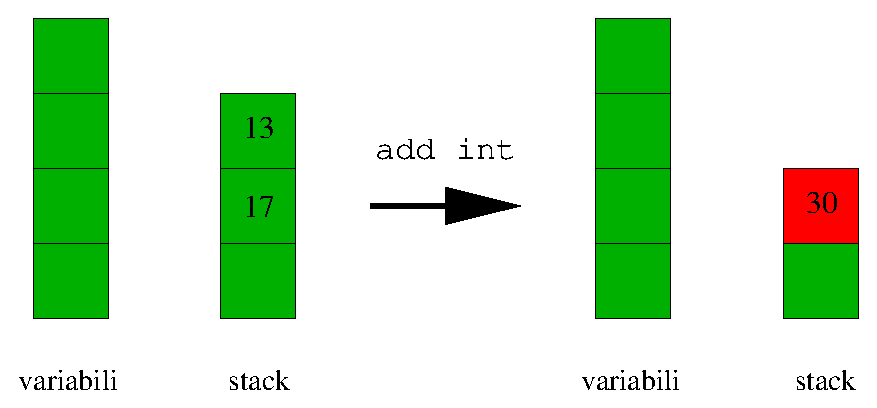
\epsfig{file = bytecodes/add.eps, width = 12cm}\\\hline
\mbox{}\\
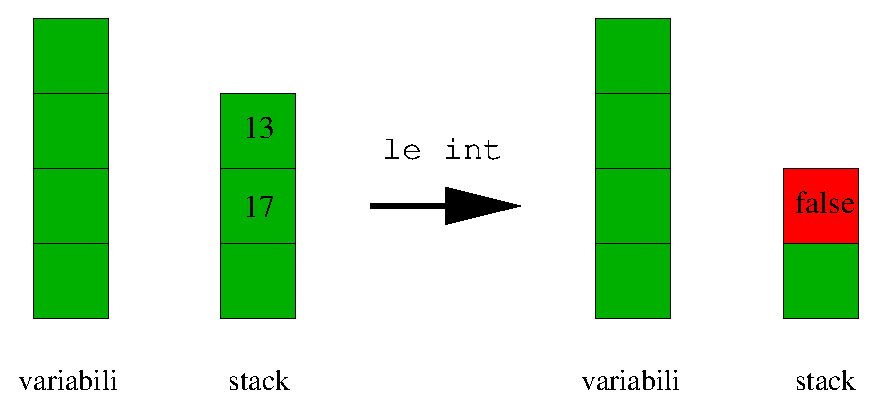
\epsfig{file = bytecodes/le.eps, width = 12cm}\\\hline
\end{tabular}
\end{center}
\caption{Le istruzioni \texttt{neg}, \texttt{add} e \texttt{le} del bytecode Kitten.}
  \label{fig:bytecodes3}
\end{figure}
%
\begin{figure}
\begin{center}
\begin{tabular}{|c|}
\hline\mbox{}\\
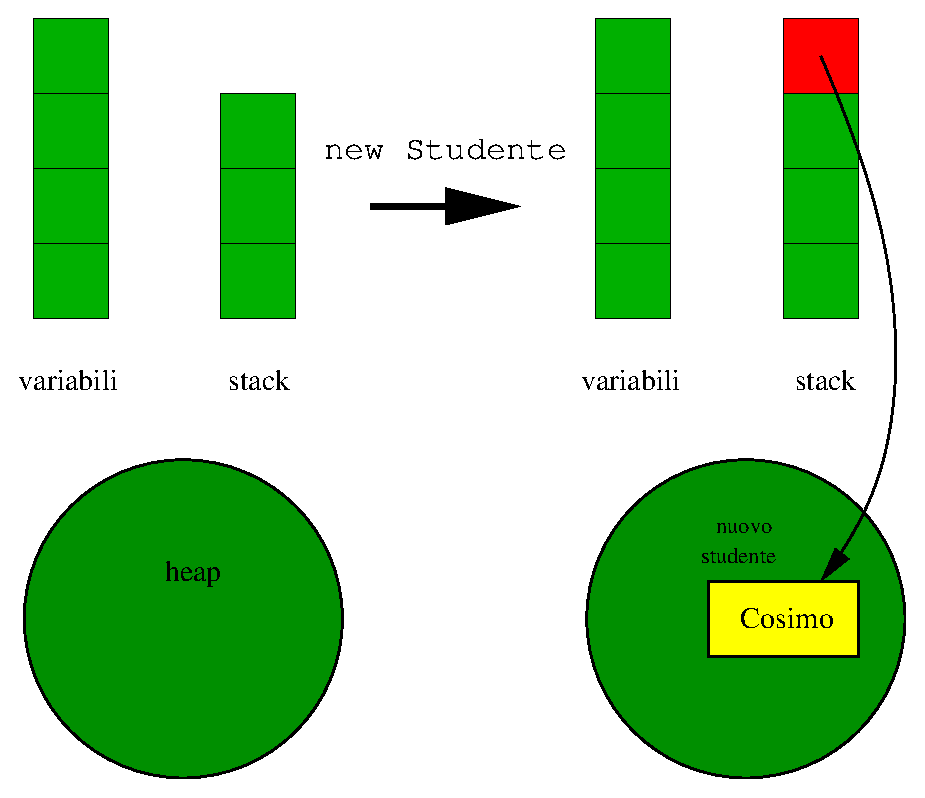
\epsfig{file = bytecodes/new.eps, width = 11.5cm}\\\hline
\mbox{}\\
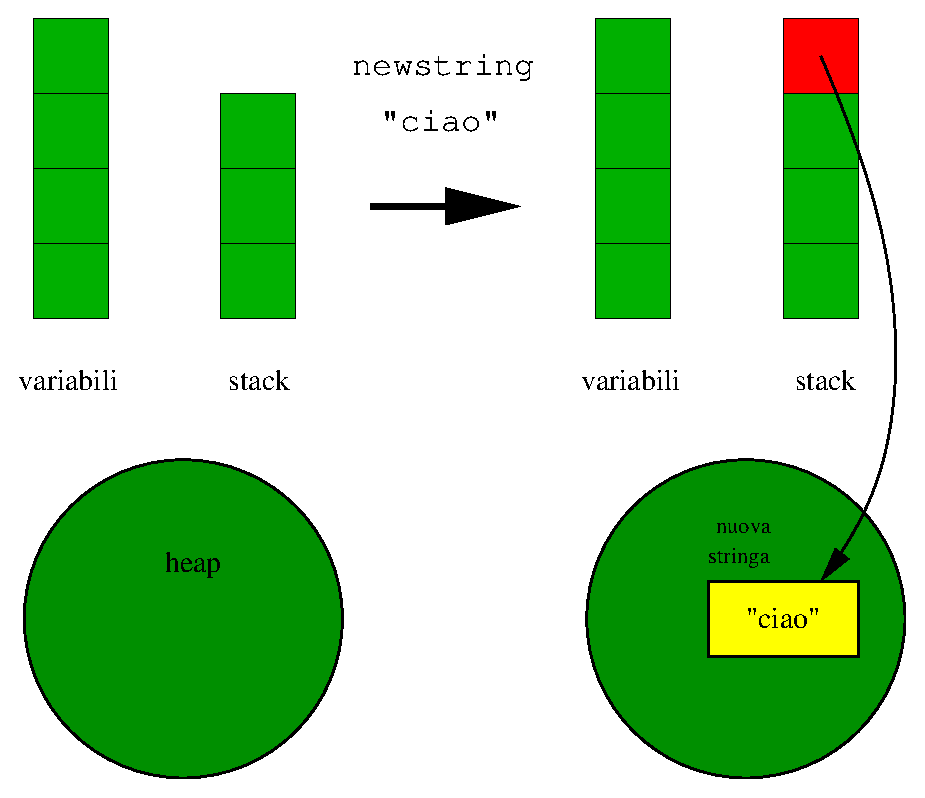
\epsfig{file = bytecodes/newstring.eps, width = 11.5cm}\\\hline
\end{tabular}
\end{center}
\caption{Le istruzioni \texttt{new} e \texttt{newstring} del bytecode Kitten.}
  \label{fig:bytecodes4}
\end{figure}
%
\begin{figure}
\begin{center}
\begin{tabular}{|c|}
\hline\mbox{}\\
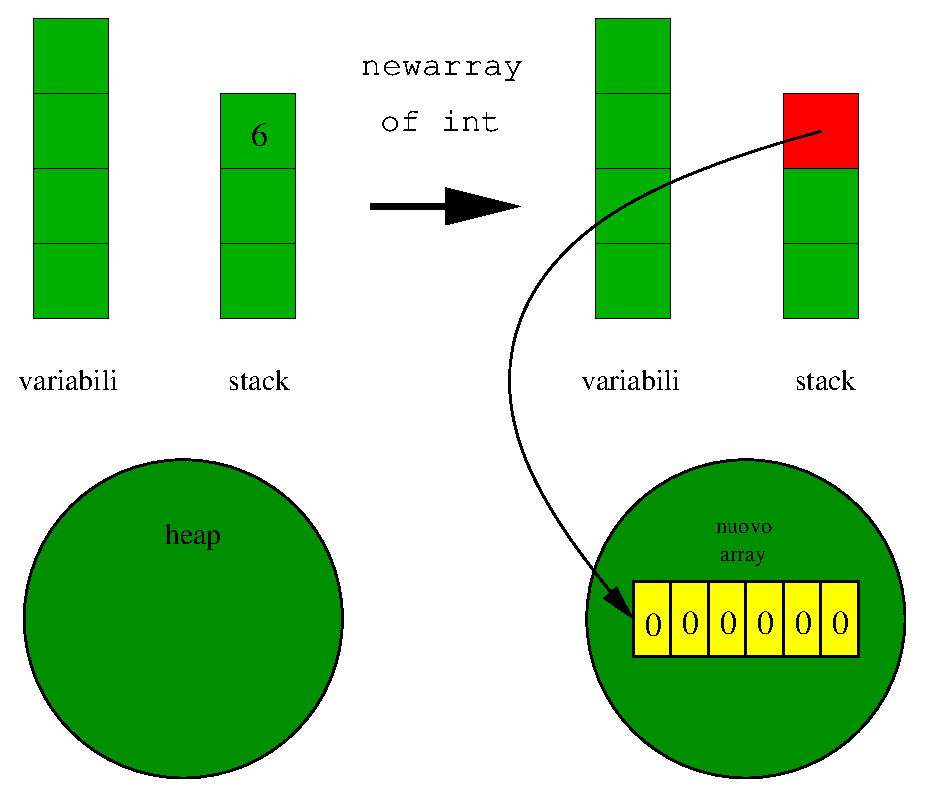
\epsfig{file = bytecodes/newarray.eps, width = 11.3cm}\\\hline
\mbox{}\\
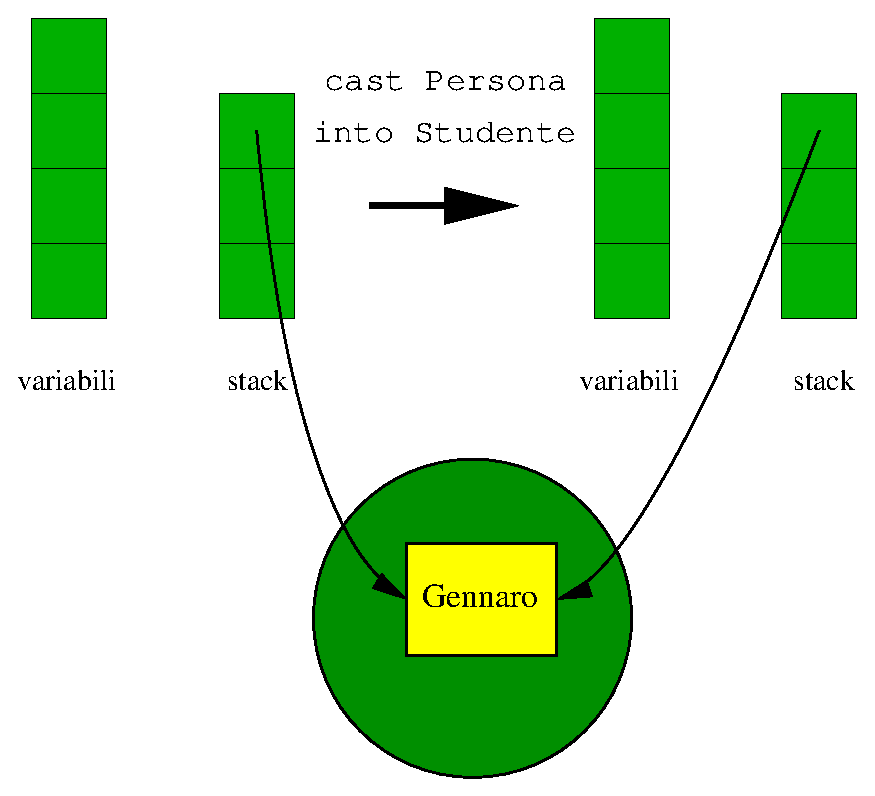
\epsfig{file = bytecodes/cast.eps, width = 11.3cm}\\\hline
\end{tabular}
\end{center}
\caption{Le istruzioni \texttt{newarray} e \texttt{cast} del bytecode Kitten.}
  \label{fig:bytecodes5}
\end{figure}
%
\begin{figure}
\begin{center}
\begin{tabular}{|c|}
\hline\mbox{}\\
\epsfig{file = bytecodes/getfield.eps, width = 12cm}\\\hline
\mbox{}\\
\epsfig{file = bytecodes/putfield.eps, width = 12cm}\\\hline
\end{tabular}
\end{center}
\caption{Le istruzioni \texttt{getfield} e \texttt{putfield} del bytecode Kitten.}
  \label{fig:bytecodes6}
\end{figure}
%
\begin{figure}
\begin{center}
\begin{tabular}{|c|}
\hline\mbox{}\\
\epsfig{file = bytecodes/arrayload.eps, width = 11.3cm}\\\hline
\mbox{}\\
\epsfig{file = bytecodes/arraystore.eps, width = 11.3cm}\\\hline
\end{tabular}
\end{center}
\caption{Le istruzioni \texttt{arrayload} e \texttt{arraystore} del bytecode Kitten.}
  \label{fig:bytecodes7}
\end{figure}
%
\begin{figure}
\begin{center}
\begin{tabular}{|c|}
\hline\mbox{}\\
\epsfig{file = bytecodes/constructorcall.eps, width = 12cm}\\\hline
\mbox{}\\
\epsfig{file = bytecodes/virtualcall.eps, width = 12cm}\\\hline
\mbox{}\\
\epsfig{file = bytecodes/return.eps, width = 12cm}\\\hline
\end{tabular}
\end{center}
\caption{Le istruzioni \texttt{constructorcall}, \texttt{virtualcall} e \texttt{return} del bytecode Kitten.}
  \label{fig:bytecodes8}
\end{figure}

Esaminiamo adesso il set di istruzioni messe a disposizione dal bytecode
Kitten. Per ognuna di esse mostriamo il suo effetto sulle variabili locali,
sullo stack degli operandi e sulla memoria o heap. Dal momento che
poche istruzioni operano sullo heap, nelle figure lo indicheremo solo per quelle poche
istruzioni per cui esso \`e effettivamente significativo.
Le istruzioni del bytecode Kitten
sono \emph{tipate}, nel senso che \e specificato il tipo
degli operandi su cui possono operare. Esse non effettuano mai una promozione
di tipo per cui, quando nella loro descrizione useremo il termine
\emph{sottotipo}, esso va inteso nel senso dell'operazione
\texttt{canBeAssignedToSpecial()} della Sezione~\ref{sec:semantical_types}.
%
\begin{description}
\item[\underline{$\mathtt{nop}$}.] Questa istruzione non modifica in nulla
  lo stato della macchina astratta. L'effetto della sua esecuzione pu\`o
  quindi essere rappresentato come in Figura~\ref{fig:bytecodes1}.
\item[\underline{$\mathtt{pop}$ $t$}.]
  Rimuove la cima dello stack degli operandi, che deve avere tipo $t$
  (Figura~\ref{fig:bytecodes1}).
\item[\underline{$\mathtt{dup}$ $t$}.] Duplica il valore in cima allo stack
  (Figura~\ref{fig:bytecodes1}) che deve avere tipo $t$.
  Si noti che se tale valore fosse un
  riferimento a un oggetto o a un array allora verrebbe duplicato il
  riferimento, creandone un alias, non l'oggetto o l'array.
\item[\underline{$\mathtt{const}\ \mathit{value}$}.]
  Carica in cima allo stack un valore
  costante (Figura~\ref{fig:bytecodes2}).
  \`E possibile caricare valori booleani, interi, float e la
  costante \texttt{nil}.
\item[\underline{$\mathtt{load\ \mathit{l}\ of\ type\ \mathit{t}}$}.]
  Carica in cima allo stack degli operandi
  una copia del valore della variabile locale
  numero $l$, che deve contenere un valore di tipo $t$
  (Figura~\ref{fig:bytecodes2}).
\item[\underline{$\mathtt{store\ \mathit{l}\ of\ type\ \mathit{t}}$}.]
  Sposta dentro la variabile locale numero $l$ il valore che si trova
  in cima allo stack degli operandi. La cima di tale stack deve contenere un
  valore del tipo $t$ e viene rimossa dall'operazione
  (Figura~\ref{fig:bytecodes2}).
\item[\underline{$\mathtt{neg\ \mathit{t}}$}.]
  Nega il valore in cima allo stack degli operandi
  (Figura~\ref{fig:bytecodes3}). Tale valore deve
  essere di tipo $t$. \`E possibile che $t$ sia \texttt{boolean},
  \texttt{int} o \texttt{float}. Si noti che il valore in cima allo
  stack che viene usato per calcolare l'operazione \texttt{neg} scompare
  dallo stack e viene sostituito dal risultato dell'operazione.
\item[\underline{$\mathtt{add\ \mathit{t}}$}.]
  Addiziona i due valori in cima allo stack degli operandi
  (Figura~\ref{fig:bytecodes3}). Tali valori devono essere entrambi di
  tipo $t$. \`E possibile che $t$ sia \texttt{int} o \texttt{float}.
  Similmente ad \texttt{add}, esistono anche le istruzioni
  \texttt{sub}, \texttt{mul} e \texttt{div}. Esistono anche le
  istruzioni \texttt{and} e \texttt{or} che per\`o operano su due
  valori di tipo \texttt{boolean}. I due valori in cima allo
  stack che sono usati per calcolare l'operazione binaria scompaiono
  dallo stack e vengono sostituiti col risultato dell'operazione.
  Si noti che questa operazione non effettua alcuna promozione di tipo,
  per cui \e vietato addizionare un intero con un numero in virgola mobile
  usando $t=\mathtt{float}$.
\item[\underline{$\mathtt{le\ \mathit{t}}$}.]
  Controlla che il valore sotto la cima dello stack degli operandi sia
  minore o uguale al valore in cima allo stesso stack e sostituisce tali due
  valori con il risultato booleano del confronto.
  (Figura~\ref{fig:bytecodes3}). I due valori devono essere di tipo $t$ pari a
  \texttt{int} o \texttt{float}.
  Esistono anche le istruzioni \texttt{lt}, \texttt{ge} e \texttt{gt}.
  Infine esistono anche le istruzioni \texttt{eq} ed \texttt{ne}, che
  possono operare su valori di tipo $t$ arbitrario, anche riferimento.
\item[\underline{$\mathtt{new\ }\mathit{\kappa}$}.]
  Crea un nuovo oggetto di classe $\kappa$.
  Un riferimento a tale oggetto viene posto in cima allo stack degli
  operandi (Figura~\ref{fig:bytecodes4}). Si noti che non viene chiamato
  alcun costruttore per l'oggetto appena creato. Esso dovr\`a essere
  chiamato successivamente con un'esplicita istruzione
  \texttt{constructorcall} (si veda dopo).
\item[\underline{$\mathtt{newstring\ }\mathit{s}$}.]
  Crea un nuovo oggetto stringa che rappresenta $s$ e pone in cima allo
  stack un riferimento all'oggetto, che \`e gi\`a inizializzato
  (Figura~\ref{fig:bytecodes4}).
\item[\underline{$\mathtt{newarray\ of\ \mathit{t}}$}.]
  Crea un array i cui elementi
  hanno tipo $t$. La lunghezza dell'array \`e specificata in cima allo stack
  degli operandi ed \`e sostituita con un riferimento all'array appena creato
  (Figura~\ref{fig:bytecodes5}).
\item[\underline{$\mathtt{cast}\ t_1\ \mathit{into}\ t_2$}.]
  Effettua il cast del valore che sta in cima allo stack, che deve avere tipo
  $t_1$, nel tipo $t_2$.
  Questo bytecode pu\`o essere usato per fare cast verso il basso di tipi
  riferimento (nel qual caso un cast errato interrompe il programma)
  o per effettuare conversioni di tipo da \texttt{int} a \texttt{float} o
  viceversa (Figura~\ref{fig:bytecodes5}).
\item[\underline{$\mathtt{getfield\ }\kappa.f$}.]
  Legge il campo $\mathit{f}$ dell'oggetto il cui riferimento \e in cima allo
  stack degli operandi. Tale riferimento viene rimosso e al suo posto viene
  messo il valore letto dal campo (Figura~\ref{fig:bytecodes6}).
  L'oggetto in cima allo stack
  deve essere di tipo $\kappa$ o di una sottoclasse di $\kappa$.
  Se tale oggetto \`e $\mathtt{nil}$ il programma viene interrotto.
\item[\underline{$\mathtt{putfield\ }\kappa.f$}.]
  Scrive il valore in cima allo stack degli operandi dentro
  il campo $f$ dell'oggetto il cui riferimento sta subito sotto
  la cima dello stack. I primi due elementi dello stack vengono rimossi
  (Figura~\ref{fig:bytecodes6}). Il valore in cima allo stack deve essere del
  tipo del campo dentro cui si sta scrivendo o di un suo sottotipo.
  L'oggetto sotto la cima dello stack
  deve essere di tipo $\kappa$ o di una sottoclasse di $\kappa$.
  Se tale oggetto \`e $\mathtt{nil}$ il programma viene interrotto.
\item[\underline{$\mathtt{arrayload\ from\ array\ of\ }\mathit{t}$}.]
  Copia in cima allo stack degli operandi il valore di un elemento di un
  array. L'indice dell'elemento \`e in cima allo stack. Subito sotto
  \`e presente il riferimento all'array
  (Figura~\ref{fig:bytecodes7}) i cui elementi hanno tipo $t$ o
  sottotipo di $t$. Se il riferimento all'array \e \texttt{nil}
  o se l'indice \e fuori dagli estremi dell'array,
  il programma viene interrotto. I primi due
  elementi in cima allo stack vengono rimossi dall'operazione e sostituiti
  con il valore letto dall'array.
\item[\underline{$\mathtt{arraystore\ into\ array\ of\ }\mathit{t}$}.]
  Scrive dentro a un array il valore che sta in cima allo stack. Sotto la cima
  dello stack c'\`e l'indice dell'elemento dell'array che deve essere scritto.
  Ancora sotto c'\`e il riferimento all'array che si sta modificando
  (Figura~\ref{fig:bytecodes7}).
  Gli elementi dell'array che si sta modificando devono essere di tipo $t$ o
  di un sottotipo di $t$. Se il riferimento all'array \e \texttt{nil}
  o se l'indice \e fuori dagli estremi dell'array,
  il programma viene interrotto. I primi tre
  elementi in cima allo stack vengono rimossi dall'operazione.
\end{description}
%
\subsection{Le istruzioni di chiamata e ritorno da metodo}
  \label{subsec:call_return}
%
La Figura~\ref{fig:bytecodes8} mostra le istruzioni usate per chiamare
un costruttore o metodo e per ritornare il controllo al chiamante.
Esse operano come segue:
%
\begin{description}
\item[\underline{$\mathtt{constructorcall\ \kappa
  (}$$\vec{t}$$\mathtt{):void}$}.]
  Chiama il costruttore della classe $\kappa$ i cui parametri formali hanno
  tipo $\vec{t}$. I parametri attuali e l'oggetto che si sta inizializzando
  (\cioe il \emph{ricevitore} dal punto di vista del chiamante e
  il parametro implicito \texttt{this} di Kitten dal punto di vista del
  chiamato) sono passati
  tramite lo stack degli operandi e vengono rimossi alla fine
  della chiamata. Questo \e mostrato in Figura~\ref{fig:bytecodes8}, dal punto
  di vista del chiamante. La classe del ricevitore deve essere $\kappa$.
  Se il ricevitore \`e $\mathtt{nil}$ l'esecuzione del programma termina.
\item[\underline{$\mathtt{virtualcall\ \kappa.\mathit{m}
  (}$$\vec{t}$$\mathtt{):\mathit{t'}}$}.]
  Chiama il metodo di nome $m$ e parametri formali di tipo $\vec{\mathit{t}}$
  cercandolo a partire dalla classe del ricevitore e risalendo nella
  catena delle superclassi. Il ricevitore e i parametri attuali della chiamata
  si trovano sullo stack al momento della chiamata e vengono rimossi
  alla fine della chiamata e sostituiti con il valore di ritorno del metodo,
  nel caso in cui $\mathit{t'}$ non sia $\mathtt{void}$. Questo \`e
  mostrato in Figura~\ref{fig:bytecodes8} dal punto di vista del chiamante.
  La classe del ricevitore deve essere $\kappa$ o una sottoclasse di $\kappa$.
  Se il ricevitore \`e $\mathtt{nil}$ l'esecuzione del programma termina.
\item[\underline{$\mathtt{return\ \mathit{t}}$}.]
  Termina l'esecuzione del metodo corrente, ritornando il controllo al
  chiamante, insieme a un eventuale valore di ritorno, che \`e la cima dello
  stack degli operandi (Figura~\ref{fig:bytecodes8}) e deve avere tipo $t$.
\end{description}
%
\begin{figure}[t]
\begin{center}
\epsfig{file = callercallee.eps, width = 12cm}
\end{center}
\caption{Il meccanismo di chiamata e ritorno da metodo.}
  \label{fig:callercallee}
\end{figure}

Il funzionamento complessivo del meccanismo di chiamata e ritorno da
costruttore o metodo \`e mostrato nella Figura~\ref{fig:callercallee}.
Il metodo chiamante prepara sullo stack degli operandi i parametri della
chiamata, incluso il ricevitore della chiamata,
indicato come $o$ in Figura~\ref{fig:callercallee}. Il metodo chiamato
\`e esplicito nel caso della chiamata a un costruttore, mentre per le chiamate
virtuali ai metodi
\`e identificato dinamicamente
a tempo di esecuzione sulla base della classe dell'oggetto a cui $o$ fa riferimento.
In entrambi i casi, esso
inizia la sua esecuzione in un frame di attivazione nuovo,
in cui le variabili locali contengono
i parametri della chiamata e lo stack degli operandi \`e vuoto.
Quando l'esecuzione del chiamato termina, se il metodo non ritorna
\texttt{void} allora la cima dello stack degli operandi del chiamato contiene
il valore di ritorno, $r$ in Figura~\ref{fig:callercallee}. La terminazione
del metodo riabilita il frame di attivazione del chiamato, in cui per\`o
lo stack degli operandi \`e stato privato dei parametri e arricchito con
il valore di ritorno $r$ del metodo.
%
\subsection{Le istruzioni di diramazione}\label{subsec:branching_bytecodes}
%
\begin{figure}[t]
\begin{center}
\begin{tabular}{|c|}
\hline\mbox{}\\
\mbox{}\\
\epsfig{file = bytecodes/if_true.eps, width = 12cm}\\\hline
\mbox{}\\
\epsfig{file = bytecodes/if_cmplt.eps, width = 12cm}\\\hline
\end{tabular}
\end{center}
\caption{Le istruzioni \texttt{if\_true} ed \texttt{if\_cmplt} del bytecode Kitten.}
  \label{fig:bytecodes9}
\end{figure}
%
Le istruzioni di diramazione
del bytecode Kitten sono sempre accoppiate all'inizio di due blocchi
di codice con lo stesso predecessore.
Esse indicano sotto quale condizione il controllo del
programma deve essere istradato verso uno dei due blocchi. Ne sono esempi le
istruzioni \texttt{if\_true} e \texttt{if\_false} in
Figura~\ref{fig:led_bytecode} e le istruzioni
\texttt{if\_cmplt int} e \texttt{if\_cmpge int} in
Figura~\ref{fig:fib_bytecode}.
Quando la condizione espressa dall'istruzione condizionale \`e vera, essa
viene eseguita, il che normalmente comporta l'eliminazione di alcuni
valori dallo stack degli operandi.

Vediamo in dettaglio l'insieme delle istruzioni di diramazione del
bytecode Kitten.
%
\begin{description}
\item[\underline{$\mathtt{if\_true}$}.]
  La condizione espressa da questa istruzione \`e che la cima dello stack degli
  operandi, che deve essere un booleano, sia il valore \texttt{true}.
  In tal caso il valore
  viene eliminato dallo stack (Figura~\ref{fig:bytecodes9}).
  Esiste anche l'istruzione simmetrica $\mathtt{if\_false}$.
\item[\underline{$\mathtt{if\_cmplt}\ t$}.]
  La condizione espressa da questa istruzione \`e che l'elemento che sta
  sotto la cima dello stack degli operandi sia minore dell'elemento che sta in
  cima allo stack. Entrambi gli elementi devono avere tipo $t$
  e vengono rimossi dallo
  stack (Figura~\ref{fig:bytecodes9}). Il tipo $t$ pu\`o essere \texttt{int}
  o \texttt{float}. Esistono anche le istruzioni $\mathtt{if\_cmple}$,
  $\mathtt{if\_cmpgt}$ ed $\mathtt{if\_cmpge}$. Esistono inoltre le
  istruzioni $\mathtt{if\_cmpeq}$ ed $\mathtt{if\_cmpne}$ la cui condizione,
  rispettivamente, \`e l'uguaglianza e la disuguaglianza dei due elementi
  in cima allo stack degli operandi. Queste ultime due istruzioni
  possono operare su tipi $t$ arbitrari, anche riferimento.
\end{description}
%
\subsection{L'implementazione del bytecode Kitten}
  \label{subsec:bytecode_implementation}
%
\begin{figure}[t]
\begin{center}
\includegraphics[width=15.5cm]{bytecodes_hierarchy.pdf}
\end{center}
\caption{La gerarchia delle classi del package \texttt{bytecode} che rappresentano le istruzioni del bytecode Kitten. Le classi ovali sono classi astratte, quelle rettangolari sono classi concrete.}
  \label{fig:bytecodes_hierarchy}
\end{figure}
%
Le istruzioni del bytecode Kitten che abbiamo descritto nelle sezioni
precedenti sono implementate nel package \texttt{bytecode}
come istanze della classe \texttt{bytecode/Bytecode.java}.
La gerarchia completa \e mostrata in Figura~\ref{fig:bytecodes_hierarchy}.
Le istruzioni vengono prima di tutto divise nelle due classi astratte
\texttt{NonBranchingBytecode} e \texttt{BranchingBytecode}.
La prima implementa le istruzioni sequenziali
delle Sezioni~\ref{subsec:sequential_bytecodes}
e~\ref{subsec:call_return}. La seconda implementa le istruzioni di
diramazione della Sezione~\ref{subsec:branching_bytecodes}.

La creazione di un bytecode avviene tramite il suo costruttore, che
richiede di specificare i tipi semantici su cui opera il bytecode.
Per esempio, un'istruzione \texttt{arrayload from array of int} si
crea con l'espressione Java
%
\begin{verbatim}
  new ARRAYLOAD(IntType.INSTANCE)
\end{verbatim}
%
La classe \texttt{bytecode/BytecodeList.java} implementa poi una lista
di bytecode che pu\`o essere inserita all'interno di un blocco di codice
(come in Figura~\ref{fig:fib_bytecode}). La struttura dati che implementa
tale blocco \e la classe \texttt{translate/CodeBlock.java} il cui costruttore
chiede di specificare la lista di bytecode contenuta nel blocco e la lista
dei successori del blocco (eventualmente vuota).

Un metodo importante della classe dei bytecode sequenziali \`e
\texttt{followedBy()}: esso richiede di specificare un blocco di codice
e restituisce un blocco ottenuto aggiungendo il bytecode in testa
al codice interno al blocco di codice. Per esempio, se il blocco di
codice $b$ contiene
%
\begin{verbatim}
  const 1
  return int
\end{verbatim}
%
allora \texttt{new IF\_TRUE().followedBy(b)} \e un blocco di codice che
contiene
%
\begin{verbatim}
  if_true
  const 1
  return int
\end{verbatim}
%
\section{La generazione del bytecode Kitten per le espressioni}
  \label{sec:expressions_bytecode_generation}
%
Mostriamo in questa sezione come tradurre
la sintassi astratta di un'espressione Kitten in del bytecode Kitten.

Abbiamo visto che un programma scritto in bytecode Kitten \`e un insieme
di blocchi all'interno dei quali si trova del codice,
come mostrato in Figura~\ref{fig:cycle_bytecode}.
Il bytecode che genereremo per le espressioni sar\`a in effetti molto
semplice, al punto che una sequenza di blocchi sar\`a
sempre sufficiente per tutte le espressioni. Si noti comunque che questa
propriet\`a
\e dovuta alla semplicit\`a delle espressioni del linguaggio Kitten e
che essa non sarebbe pi\`u vera se Kitten ammettesse ad esempio espressioni pi\`u
complesse, come l'espressione condizionale
$\mathit{exp}\ \mathtt{?}\ \mathit{exp}\ \mathtt{:}\ \mathit{exp}$
(si veda l'Esercizio~\ref{ex:conditional_expression_compilation}).

Ci sono tre contesti in cui un'espressione Kitten pu\`o trovarsi:
%
\begin{enumerate}
\item un contesto in cui di un'espressione serve il valore, come
      nel caso in cui essa occorre come lato destro di un assegnamento;
\item un contesto in cui di un'espressione serve sapere se \e vera o falsa
      per decidere come istradare l'esecuzione del programma, come nel
      caso in cui essa occorre come test di un condizionale. Ovviamente
      questo caso ha senso solo per le espressioni booleane;
\item un contesto in cui il valore di un'espressione deve essere modificato,
      come nel caso in cui essa occorre alla sinistra di un assegnamento.
      Ovviamente questo caso ha senso solo per i leftvalue.
\end{enumerate}
%
Compileremo un'espressione in tre modi diversi,
sulla base del contesto in cui essa occorre. Tali modi
sono detti rispettivamente
\emph{compilazione attiva}, \emph{compilazione condizionale} e
\emph{compilazione passiva} dell'espressione. Descriviamo adesso in
ordine questi tre tipi di compilazione delle espressioni.
%
\subsection{La compilazione attiva delle espressioni}
  \label{subsec:active_compilation}
%
Quando di un'espressione ci interessa il valore, allora l'esecuzione
del codice che vogliamo generare deve essere tale da:
%
\begin{enumerate}
\item lasciare intatti i valori iniziali sullo stack degli operandi;
\item aggiungere in cima allo stack degli operandi il valore dell'espressione.
\end{enumerate}
%
Questi due principi sono mostrati in Figura~\ref{fig:russian}. Il
vincolo 1 \`e importante poich\'e esso ci permette di valutare
in sequenza delle espressioni e ritrovarci alla fine i loro
valori sullo stack.
Questo \`e mostrato nella Figura~\ref{fig:russian_relevance},
che mostra l'esecuzione del codice che genereremo per l'and logico
di due espressioni $e_1$ ed $e_2$: prima generiamo del codice che
valuta $e_1$ e ne lascia il valore sullo stack, poi del codice che
valuta $e_2$ e ne lascia il valore sullo stack. Grazie al precedente vincolo
1, siamo certi che a questo punto il valore di $e_1$ \`e ancora nello stack,
sotto la cima. Possiamo quindi aggiungere un bytecode \texttt{and} per
ottenere il risultato cercato.

\begin{figure}[t]
\begin{center}
\epsfig{file = russe.eps, width = 8cm}
\end{center}
\caption{L'esecuzione del bytecode Kitten generato per un'espressione deve lasciare il valore dell'espressione sullo stack degli operandi e non deve modificare lo stack iniziale.}
  \label{fig:russian}
\end{figure}
%
\begin{figure}[t]
\begin{center}
\epsfig{file = importanza.eps, width = 12cm}
\end{center}
\caption{L'esecuzione del bytecode Kitten per l'and logico di due espressioni $e_1$ ed $e_2$.}
  \label{fig:russian_relevance}
\end{figure}

Se $\beta$ \`e un blocco di codice, allora con la notazione
$\fbox{$\mathit{ins}$}\to\beta$
rappresentiamo un blocco di codice
al cui interno si trova l'istruzione (o le istruzioni) $\mathit{ins}$
e che ha $\beta$ come successore.
La Figura~\ref{fig:expressions_generation} usa tale notazione per
definire le regole per la
generazione del codice per le espressioni Kitten. Esse sono formalizzate
tramite una funzione $\gen{\_}$ che associa alla sintassi astratta
delle espressioni il bytecode Kitten che ne calcola il valore e lo lascia
in cima allo stack degli operandi.
Tale funzione richiede in primo luogo di specificare l'espressione $e$
di cui si vuole generare il bytecode. La notazione $\gen{e}$ \`e
per\`o ancora una funzione da $\mathtt{translate.CodeBlock}$ in
$\mathtt{translate.CodeBlock}$, \cioe la classe usata per
rappresentare un blocco di bytecode
(Sezione~\ref{subsec:bytecode_implementation}). In particolare, quello che
occorre ancora specificare \`e il bytecode $\beta$
che deve essere eseguito \emph{dopo} la valutazione di $e$.
Il bytecode $\gen{e}(\beta)$ sar\`a quindi il bytecode che \emph{prima}
valuta l'espressione $e$, lasciandone il valore sullo stack degli operandi,
e \emph{dopo} esegue il codice $\beta$. Per esempio, la
Figura~\ref{fig:expressions_generation} implica che
\[
  \gen{\mathtt{IntLiteral(3)}}(\fbox{$\mathtt{return\ int}$})
    =\fbox{$\mathtt{const\ 3}$}\to\fbox{$\mathtt{return\ int}$}
\]

Questo modo di generare il codice
si chiama \emph{compilazione con continuazioni} e $\beta$ \`e detta
la \emph{continuazione} della compilazione di $e$. La compilazione per
continuazioni \`e molto elegante \poiche permette di semplificare la fusione
fra il codice generato per due parti sequenziali di un programma.
%
\begin{figure}[t]
{\scriptsize
\begin{align*}
  \gen{\_}:\mathtt{absyn.Expression}&\mapsto(\mathtt{translate.CodeBlock}\mapsto\mathtt{translate.CodeBlock})\\
  \mbox{}\\
  \gen{\mathtt{Variable(\mathit{name})}}(\beta)&=\fbox{\texttt{load $\mathit{num}$ of type $\tau$}}\to\beta\\
  \text{dove $\mathit{num}$ \`e il numero}&\text{ progressivo della variabile \textit{name} nel metodo corrente}\\
  \gen{\mathtt{FieldAccess(\mathit{receiver},\mathit{name})}}(\beta)&=
    \gen{\mathit{receiver}}\left(\fbox{\texttt{getfield $\mathit{field}$}}
    \to\beta\right)\\
  \text{dove $\mathit{field}$ \`e il campo}&\text{ identificato
    dall'analisi semantica (Figura~\ref{fig:analysis_expressions1})}\\
  \gen{\mathtt{ArrayAccess(\mathit{array},\mathit{index})}}(\beta)&=
    \gen{\mathit{array}}\left(\gen{\mathit{index}}\left(
    \fbox{$\mathtt{arrayload\ from\ array\ of\ }\tau$}\to\beta\right)\right)\\
  \gen{\mathtt{True()}}(\beta)=\fbox{$\mathtt{const\ true}$}\to\beta&\qquad
  \gen{\mathtt{False()}}(\beta)=\fbox{$\mathtt{const\ false}$}\to\beta\\
  \gen{\mathtt{IntLiteral(\mathit{value})}}(\beta)
    &=\gen{\mathtt{FloatLiteral(\mathit{value})}}(\beta)
    =\fbox{$\mathtt{const}\ \mathit{value}$}\to\beta\\
  \gen{\mathtt{String(\mathit{value})}}(\beta)
    =\fbox{$\mathtt{newstring}\ \mathit{value}$}\to\beta&\qquad
    \gen{\mathtt{Nil()}}(\beta)=\fbox{$\mathtt{const\ nil}$}\to\beta\\
  \gen{\mathtt{NewObject(\mathit{className},\mathit{actuals})}}(\beta)
    &=\fbox{$\begin{array}{l}
      \mathtt{new}\ \kappa\\
      \mathtt{dup}\ \kappa
    \end{array}$}\to
   \gentwo{\vec{t}}{\mathit{actuals}}
   \left(\fbox{$\mathtt{constructorcall}\ \mathit{con}$}\to\beta\right)\\
  \text{dove $\mathit{con}=\kappa(\vec{t})\mathtt{:void}$ \e il}&
  \text{ costruttore identificato dall'analisi semantica
        (Figura~\ref{fig:analysis_expressions2})}\\
  \gen{\mathtt{NewArray(\mathit{elementsType},\mathit{size})}}(\beta)
    &=\gen{\mathit{size}}
    \left(\fbox{$\mathtt{newarray\ of\ }\tau\mathtt{.getElementsType()}$}
    \to\beta\right)\\
  \gen{\mathtt{MethodCallExpression(\mathit{receiver},\mathit{name},
    \mathit{actuals})}}&=\gen{\mathit{receiver}}\left(
    \gentwo{\vec{t}}{\mathit{actuals}}
    \left(\fbox{$\mathtt{virtualcall}\ \mathit{method}$}
    \to\beta\right)\right)\\
  \text{dove $\mathit{method}=\kappa.\mathtt{m}(\vec{t}):t'$
        \`e il}&
  \text{ metodo identificato dall'analisi semantica
        (Figura~\ref{fig:analysis_expressions2})}\\
  \gen{\mathtt{Not(\mathit{expression})}}(\beta)=
    \gen{\mathtt{Minus(\mathit{expression})}}(\beta)&=
    \gen{\mathit{expression}}\left(
    \fbox{$\mathtt{neg\ }\tau$}\to\beta\right)\\
  \gen{\mathtt{Cast(\mathit{\mathit{type},\mathit{expression}})}}(\beta)=
      \gen{\mathit{expression}}&
        \left(\fbox{$\mathtt{cast\ from\ }\tau'\mathtt{\ into\ }\tau$}
        \to\beta\right)
  \quad\text{con $\tau'$ \e tipo statico di }\mathit{expression}\\
  \gen{\mathtt{And(\mathit{left},\mathit{right})}}(\beta)&=
    \gen{\mathit{left}}\left(
      \gen{\mathit{right}}\left(\fbox{$\mathtt{and}$}\to\beta\right)\right)\\
  \gen{\mathtt{Addition(\mathit{left},\mathit{right})}}(\beta)&=
    \gentwo{\tau}{\mathit{left}}\left(
      \gentwo{\tau}{\mathit{right}}\left(\fbox{$\mathtt{add}\ \tau$}
      \to\beta\right)\right)\\
  \gen{\mathtt{LessThanOrEqual(\mathit{left},\mathit{right})}}(\beta)=
    \gentwo{\ell}{\mathit{left}}\Big(
      \gentwo{\ell}{\mathit{right}}&\left(\fbox{$\mathtt{le}\ \ell$}
      \to\beta\right)\Big)\quad
  \text{con $\ell$ minimo supertipo comune fra il tipo statico di
    $\mathit{left}$ e di $\mathit{right}$}
\end{align*}
}
\caption{La funzione $\gen{\_}$ che genera il bytecode Kitten che valuta le espressioni. Il tipo $\tau$ \`e il tipo statico assegnato all'espressione durante la sua analisi semantica.}
  \label{fig:expressions_generation}
\end{figure}

La Figura~\ref{fig:expressions_generation} usa la funzione
$\gentwo{\tau}{e}$ che rispetto a $\gen{e}$ effettua in pi\`u,
se necessario, la promozione a $\tau$ del valore dell'espressione $e$.
In Kitten essa \e utile ogni qual volta si usa un valore intero
in un punto in cui si richiedeva un valore in virgola mobile come
per esempio nell'espressione $\mathtt{3\ +\ 4.5}$, in cui occorre convertire
il valore intero $3$ in un $\mathtt{float}$ prima di sommarlo con
il valore $4.5$. Quando potrebbe essere necessaria una promozione di tipo
del valore di un'espressione, la Figura~\ref{fig:expressions_generation}
compila l'espressione tramite $\gentwo{\tau}{\_}$ piuttosto
che tramite $\gen{\_}$.
Lo stesso fenomeno lo incontreremo fra poco con i comandi,
in un assegnamento del tipo:
%
\begin{verbatim}
  float f := 13
\end{verbatim}
%
dove l'intero $13$ deve essere convertito in \texttt{float} prima
dell'assegnamento.
Tale funzione di conversione \`e definita a partire da $\gen{e}$:
\begin{equation}\label{eq:gentwo}
  \gentwo{\tau}{e}(\beta)=\begin{cases}
    \gen{e}(\fbox{$\mathtt{cast\ from\ int\ into\ float}$}\to\beta) &
      \text{se $\tau$ \`e $\mathtt{float}$ ed
            $e$ ha tipo statico $\mathtt{int}$}\\
    \gen{e}(\beta) & \text{altrimenti.}
  \end{cases}
\end{equation}
Per esempio,
%
\begin{align*}
  \gentwo{\mathtt{int}}{\mathtt{IntLiteral(3)}}(\fbox{$\mathtt{return\ int}$})
    &=\gen{\mathtt{IntLiteral(3)}}(\fbox{$\mathtt{return\ int}$})\\
  &=\fbox{$\mathtt{const\ 3}$}\to\fbox{$\mathtt{return\ int}$}
\end{align*}
%
mentre
%
\begin{align*}
  &\quad\gentwo{\mathtt{float}}{\mathtt{IntLiteral(3)}}
    (\fbox{$\mathtt{return\ float}$})\\
  &=\gen{\mathtt{IntLiteral(3)}}(\fbox{$\mathtt{cast\ from\ int\ into\ float}$}
    \to\fbox{$\mathtt{return\ float}$})\\
  &=\fbox{$\mathtt{const\ 3}$}\to\fbox{$\mathtt{cast\ from\ int\ into\ float}$}
    \to\fbox{$\mathtt{return\ float}$.}
\end{align*}
%
L'esempio precedente sarebbe quello di un'istruzione
$\mathtt{return\ 3}$ che occorre all'interno di un metodo il cui
tipo di ritorno \`e $\mathtt{float}$.
La notazione $\gentwo{\tau}{\_}$ viene infine
estesa a sequenze di espressioni e di tipi (di uguale lunghezza),
ottenendo la notazione $\gentwo{\vec{t}}{\_}$, definita come segue:
%
\begin{align*}
  \gentwo{\epsilon}{\mathtt{null}}(\beta)&=\beta\\
  \gentwo{\tau::\vec{t}}{\mathtt{ExpressionSeq(\mathit{head},
    \mathit{tail})}}(\beta)&=\gentwo{\tau}{\mathit{head}}(\gentwo{\vec{t}}
    {\mathit{tail}}(\beta))~.
\end{align*}
%
Per esempio:
%
{\small
\begin{align*}
  &\hspace*{-5ex}\gentwotwo{\mathtt{float}::\mathtt{float}}
    {\begin{array}{c}
     \mathtt{ExpressionSeq(FloatLiteral(3.4),}\\
     \mathtt{ExpressionSeq(IntLiteral(4),null))}
     \end{array}}
    (\fbox{$\mathtt{add\ float}$})\\
  &=\gentwo{\mathtt{float}}{\mathtt{FloatLiteral(3.4)}}
    (\gentwo{\mathtt{float}}{\mathtt{IntLiteral(4)}}
    (\fbox{$\mathtt{add\ float}$}))\\
  &=\gentwo{\mathtt{float}}{\mathtt{FloatLiteral(3.4)}}
    (\fbox{$\mathtt{const\ 4}$}\to\fbox{$\mathtt{cast\ from\ int\ to\ float}$}
    \to\fbox{$\mathtt{add\ float}$})\\
  &=\fbox{$\mathtt{const\ 3.4}$}
    \to\fbox{$\mathtt{const\ 4}$}\to\fbox{$\mathtt{cast\ from\ int\ to \ float}$}
    \to\fbox{$\mathtt{add\ float}$.}
\end{align*}}

Commentiamo adesso le regole di generazione del bytecode Kitten in
Figura~\ref{fig:expressions_generation}.
%
\begin{description}
\item[\underline{$\mathtt{Variable(\mathit{name})}$}.]
  Per caricare sullo stack il valore di una variabile locale, usiamo
  il bytecode \texttt{load} della Figura~\ref{fig:bytecodes2}.
  Il numero della variabile locale \`e gi\`a stato determinato in
  fase di analisi semantica e accessibile tramite il type-checker usato
  per l'analisi, insieme al tipo della variabile
  (Figura~\ref{fig:semantical.TypeChecker}).
\item[\underline{$\mathtt{FieldAccess(\mathit{receiver},\mathit{name})}$}.]
  Per accedere a un campo dell'oggetto $o$
  contenuto in $\mathit{receiver}$,
  generiamo inizialmente il bytecode che lascia sullo stack degli operandi
  il riferimento ad $o$. Questo \`e ottenuto richiamando ricorsivamente
  la generazione del bytecode per $\mathit{receiver}$. Come continuazione,
  gli passiamo un blocco che contiene un bytecode
  $\mathtt{getfield}$ (Figura~\ref{fig:bytecodes6})
  e che \`e legato alla continuazione $\beta$.
  L'effetto globale \`e quindi quello di valutare $\mathit{receiver}$,
  leggere il valore del campo di nome $\mathit{name}$ e quindi continuare
  con la continuazione $\beta$. Si noti che il campo da leggere \`e gi\`a
  stato identificato in fase di analisi semantica ($\mathit{field}$ in
  Figura~\ref{fig:analysis_expressions1}).
\item[\underline{$\mathtt{ArrayAccess(\mathit{array},\mathit{index})}$}.]
  Leggere un elemento di un array richiede in primo luogo di
  valutare l'espressione che contiene il riferimento all'array. Questo \`e
  ottenuto compilando ricorsivamente $\mathit{array}$. Come continuazione
  gli diamo la compilazione di $\mathit{index}$, seguita dal bytecode
  $\mathtt{arrayload}$ e dalla
  continuazione $\beta$. Si noti che il tipo statico $\tau$
  dell'array \`e gi\`a stato calcolato in fase di analisi semantica.
  Il bytecode $\mathtt{arrayload}$ consumer\`a dallo stack
  il riferimento all'array e l'indice da cui leggere e li sostituir\`a
  con il valore dell'elemento letto (Figura~\ref{fig:bytecodes7}).
\item[\underline{$\mathtt{True()}$},
      \underline{$\mathtt{False()}$},
      \underline{$\mathtt{IntLiteral(\mathit{value})}$},
      \underline{$\mathtt{FloatLiteral(\mathit{value})}$},
      \underline{$\mathtt{String(\mathit{value})}$},
      \underline{$\mathtt{Nil()}$}.]
  Dal mo-\linebreak
  mento che queste
  classi di sintassi astratta rappresentano delle costanti,
  usiamo il bytecode $\mathtt{const}$ della Figura~\ref{fig:bytecodes2}
  e $\mathtt{newstring}$ della Figura~\ref{fig:bytecodes4} per caricare tali
  costanti in cima allo stack.
\item[\underline{$\mathtt{NewObject(\mathit{className,\mathit{actuals}})}$}.]
  Questo nodo di sintassi astratta per la creazione di un oggetto di classe
  $\mathit{className}$ \e stato annotato durante l'analisi semantica con
  il costruttore $\mathit{con}=
  \kappa(\vec{t})\mathtt{:void}$ della classe $\kappa$ che \`e
  il corrispondente semantico di $\mathit{className}$. Tale costruttore
  \e il \piu
  specifico fra quelli che possono essere chiamati da questa espressione
  sulla base del tipo
  statico dei parametri attuali (Figura~\ref{fig:analysis_expressions2}).
  Il codice che generiamo inizia con un bytecode $\mathtt{new}\ \kappa$ che
  crea un nuovo oggetto $o$ di classe $\kappa$ e ne pone in cima allo stack
  un riferimento (Figura~\ref{fig:bytecodes4}). Tale riferimento
  viene quindi duplicato dal bytecode $\mathtt{dup}\ \kappa$
  (Figura~\ref{fig:bytecodes1}).
  Segue la compilazione dei parametri attuali del costruttore.
  A questo punto sullo stack troviamo due copie di un riferimento
  ad $o$ sormontate dai valori dei parametri
  attuali. Con il bytecode \texttt{constructorcall} otteniamo quindi di
  chiamare il costruttore legando $\mathtt{this}$ ad $o$ e i parametri
  attuali ai parametri formali (Figura~\ref{fig:bytecodes8}).
  Per esempio, la compilazione di
  \begin{multline*}
    \mathtt{NewObject(\mathit{className},}\\
    \mathtt{ExpressionSeq(IntLiteral(3),ExpressionSeq(IntLiteral(4),null)))}
  \end{multline*}
  \e
  \[\begin{array}{l}
    \mathtt{new}\ \kappa\\
    \mathtt{dup}\ \kappa\\
    \mathtt{const\ 3}\\
    \mathtt{const\ 4}\\
    \mathtt{constructorcall\ \mathit{con}}
  \end{array}\]
  seguita dalla continuazione $\beta$ (nell'ipotesi che non serva promozione
  di tipo nel passaggio dei parametri interi al costruttore).
  Dalla Figura~\ref{fig:bytecodes8} sappiamo che
  il bytecode \texttt{constructorcall}
  rimuove dallo stack degli operandi sia i parametri attuali che $o$.
  Questo \`e il motivo per cui usiamo il bytecode $\mathtt{dup}$:
  senza di esso il riferimento ad $o$ andrebbe perso dallo stack
  e avremmo ottenuto di inizializzare un oggetto che subito dopo
  diventava irraggiungibile.
\item[\underline{$\mathtt{NewArray(\mathit{elementsType},\mathit{size})}$}.]
  Il bytecode generato per la creazione di un array inizia con
  la compilazione dell'espressione $\mathit{size}$ che lascia in cima allo
  stack la dimensione richiesta per l'array.
  Basta quindi proseguire il codice con un bytecode $\mathtt{newarray}$ che
  consuma tale dimensione e la sostituisce con un riferimento a un nuovo
  array (Figura~\ref{fig:bytecodes5}). Segue la continuazione $\beta$.
  Si ricordi che il tipo statico $\tau$ di questa espressione \`e il tipo
  dell'array che stiamo creando (Figura~\ref{fig:analysis_expressions2}).
\item[\underline{$\mathtt{MethodCallExpression(\mathit{receiver},\mathit{name},
  \mathit{actuals})}$}.]
  L'invocazione di un metodo \`e compilata in modo molto simile all'invocazione
  di un costruttore per un nodo $\mathtt{NewObject}$ di sintassi astratta
  (si veda sopra). La differenza \`e che si usa il bytecode
  $\mathtt{virtualcall}$ invece di $\mathtt{constructorcall}$
  (Figura~\ref{fig:bytecodes8}). Inoltre il riferimento all'oggetto
  ricevitore della chiamata \`e il valore lasciato sullo stack dal
  bytecode generato per $\mathit{receiver}$, piuttosto che un nuovo oggetto
  come per $\mathtt{NewObject}$. Si ricordi che l'analisi semantica ha
  garantito che il metodo invocato ha un tipo di ritorno diverso da
  $\mathtt{void}$ (Figura~\ref{fig:analysis_expressions2}). Siamo quindi
  sicuri che il bytecode $\mathtt{virtualcall}$ lascia sullo stack un
  valore di ritorno (Figura~\ref{fig:bytecodes8}), che \`e il valore di
  questa espressione d'invocazione di un metodo.
\item[\underline{$\mathtt{Not(\mathit{expression})}$} e
  \underline{$\mathtt{Minus(\mathit{expression})}$}.]
  Entrambe queste espressioni sono compilate in del bytecode che
  inizia con la compilazione ricorsiva di $\mathit{expression}$ e continua
  con il bytecode $\mathtt{neg}$ (Figura~\ref{fig:bytecodes3})
  e con la continuazione $\beta$. Si noti comunque che il tipo $\tau$
  su cui opera $\mathtt{neg}$ \`e diverso: esso \`e $\mathtt{boolean}$
  per $\mathtt{Not}$ ed \`e $\mathtt{int}$ oppure $\mathtt{float}$ per
  $\mathtt{Minus}$ (Figura~\ref{fig:analysis_expressions2}).
\item[\underline{$\mathtt{Cast(\mathit{type},\mathit{expression})}$}.]
  La compilazione di un cast verso il basso \`e essenzialmente la compilazione
  dell'espressione di cui si sta facendo il cast, seguita dalla continuazione
  $\beta$. In \piu inseriamo un bytecode $\mathtt{cast}$
  che effettua il cast o la conversione di tipo da
  $\mathtt{float}$ ad $\mathtt{int}$ (Figura~\ref{fig:bytecodes5})
  nel caso in cui il cast sia in effetti
  una richiesta di arrotondamento di un valore a virgola mobile
  ($\mathtt{3.14\ as\ int}$). Si noti la differenza fra queste due
  situazioni: la conversione da $\mathtt{float}$ a $\mathtt{int}$
  modifica la rappresentazione binaria del valore in cima allo stack ma
  non pu\`o mai fallire (sappiamo con certezza che in cima allo stack
  c'\`e un $\mathtt{float}$). La verifica di tipo non effettua invece
  alcuna modifica sul valore in cima allo stack, ma pu\`o fallire
  bloccando l'esecuzione del programma.
\item[\underline{$\mathtt{BinOp(\mathit{left},\mathit{right})}$}.]
  La compilazione di un'operazione binaria \`e il codice formato
  dalla compilazione di $\mathit{left}$ seguita dalla compilazione
  di $\mathit{right}$ seguita da un bytecode che implementa
  l'operazione binaria opportuna e infine dalla continuazione $\beta$.
  Gli esempi mostrati in Figura~\ref{fig:expressions_generation}
  presentano tutte le tipologie di espressioni binarie.
  Quelle logiche usano un bytecode $\mathtt{and}$ od $\mathtt{or}$ per
  il quale non serve specificare il tipo degli operandi (\`e sempre
  $\mathtt{boolean}$). Quelle aritmetiche possono invece
  operare sia su $\mathtt{int}$ che su $\mathtt{float}$ e i loro
  operandi potrebbero richiedere una promozione di tipo, per cui usiamo
  per essi $\gentwo{\tau}{\_}$ piuttosto che $\gen{\_}$. Le operazioni
  binarie di confronto possono operare su tipo arbitrari e possono
  anch'esse richiedere una conversione di tipo per gli operandi.
\end{description}

Consideriamo adesso l'implementazione delle regole di compilazione
in Figura~\ref{fig:expressions_generation}. Un blocco di codice
lo implementiamo come un oggetto di classe
$\mathtt{translate.CodeBlock}$ contenente una lista
di bytecode Kitten ed eventualmente legato ad altri blocchi successori.
L'implementazione della funzione $\gamma$ \e
ottenuta tramite i seguenti due metodi aggiunti
ad $\mathtt{absyn/Expression.java}$:
%
\begin{verbatim}
  protected abstract CodeBlock translate(CodeBlock continuation);

  public final CodeBlock translateAs(Type type, CodeBlock continuation) {
    if (staticType == IntType.INSTANCE && type == FloatType.INSTANCE)
      continuation = new CAST(IntType.INSTANCE, FloatType.INSTANCE)
                       .followedBy(continuation);
    else
      return translate(continuation);
  }
\end{verbatim}
%
Il primo implementa $\gen{\_}$ ed
\`e lasciato \texttt{abstract}. Esso verr\`a istanziato nelle
sottoclassi di $\mathtt{absyn.Expression}$
con l'implementazione delle regole in
Figura~\ref{fig:expressions_generation}. Il secondo implementa la funzione
$\gentwo{\tau}{\_}$ dell'Equazione~\ref{eq:gentwo}. Si noti l'uso di
\texttt{followedBy()} per aggiungere un bytecode in cima a un blocco di codice.

Mostriamo alcuni esempi di istanziazione del metodo
$\mathtt{translate()}$. In \texttt{absyn/True.java} definiamo
%
\begin{verbatim}
  public final CodeBlock translate(CodeBlock continuation) {
    return new CONST(true).followedBy(continuation);
  }
\end{verbatim}
%
che rispecchia fedelmente quanto riportato in
Figura~\ref{fig:expressions_generation}.

In \texttt{absyn/Variable.java} defininiamo
%
\begin{verbatim}
  public CodeBlock translate(CodeBlock continuation) {
    return new LOAD(getVarNum(), getStaticType()).followedBy(continuation);
  }
\end{verbatim}
%
Il numero della variabile era stato annotato in fase di analisi semantica
(Sezione~\ref{subsec:analysis_expressions_implementation}).
Utilizziamo anche il tipo
$\tau$ annotato per questa espressione, accessibile tramite
\texttt{getStaticType()}. Ancora una volta, questa implementazione
riflette la definizione in Figura~\ref{fig:expressions_generation}.

Dentro \texttt{absyn/BinOp.java} definiamo
%
\begin{verbatim}
  public final CodeBlock translate(CodeBlock continuation) {
    Type ell = getLeft().getStaticType()
      .leastCommonSupertype(getRight().getStaticType());
    return getLeft().translateAs
      (ell, getRight().translateAs
       (ell, operator(ell).followedBy(continuation)));
  }

  protected abstract BinOpBytecode operator(Type type);
\end{verbatim}
%
L'idea \`e di calcolare il minimo sovratipo comune $\ell$
fra i tipi statici dei due operandi, compilarli entrambi con
$\gentwo{\mathit{\ell}}{\_}$ e farli quindi seguire da un bytecode binario
specifico all'operazione binaria che si sta compilando. Tale bytecode
\`e fornito dal metodo ausiliario \texttt{operator()} che \`e per esempio
definito dentro $\mathtt{absyn/Addition.java}$ come
%
\begin{verbatim}
  protected BinOpBytecode operator(Type type) {
    return new ADD((NumericalType) type);
  }
\end{verbatim}
%
Si noti che questo modo di procedere generalizza le tre ultime regole
in Figura~\ref{fig:expressions_generation}.
%
\subsection{La compilazione condizionale delle espressioni booleane}
  \label{subsec:conditional_generation}
%
Abbiamo descritto come un'espressione venga tradotta in del bytecode
Kitten che ne calcola il valore e lo lascia in cima allo stack degli
operandi. Tale codice \e adeguato se quello a cui
siamo interessati \`e il valore dell'espressione. Per esempio, di un parametro
passato a un metodo abbiamo bisogno del valore, \cosi come del lato destro
di un assegnamento.
Ci sono casi per\`o in cui quello che ci interessa \`e di istradare
l'esecuzione di un programma in due direzioni diverse sulla base
del valore di un'espressione booleana. Per esempio, nel comando
$\mathtt{if\ (\mathit{exp})\ then\ \mathit{com}_{\rm 1}
\ else\ \mathit{com}_{\rm 2}}$
siamo interessati a eseguire $\mathit{com}_1$ se il valore
di $\mathit{exp}$ \`e $\mathit{true}$ e a eseguire $\mathit{com}_2$
se tale valore \`e invece $\mathit{false}$. Occorre quindi definire
un altro modo di generare il bytecode per le espressioni,
alternativo a quello della
Figura~\ref{fig:expressions_generation} e che chiameremo
\emph{compilazione condizionale} delle espressioni. Va comunque detto che
ricicleremo in larghissima misura le definizioni in tale figura. Va ricordato
inoltre che
la compilazione condizionale ha senso solo per le espressioni che hanno
tipo \texttt{boolean},
dal momento che l'analisi semantica ci garantisce che esse sono le uniche
che possono essere usate nei test dei condizionali e dei cicli
(Figura~\ref{fig:analysis_expressions2}).

Definiamo quindi una funzione
%
\begin{multline*}
  \gentest{\_}{}{}:\mathtt{absyn.Expression}\to
    \mathtt{translate.CodeBlock}\\
  \mapsto\mathtt{translate.CodeBlock}
    \mapsto\mathtt{translate.CodeBlock}
\end{multline*}
%
che compila un'espressione in maniera condizionale.
In particolare, $\gentest{\mathit{exp}}(\beta_\mathit{true})
(\beta_\mathit{false})$ \`e la
compilazione condizionale dell'espressione $\mathit{exp}$:
se l'espressione contiene $\mathit{true}$ l'esecuzione
viene istradata verso la continuazione $\beta_\mathit{true}$;
altrimenti verso la continuazione $\beta_\mathit{false}$.
La sua definizione sfrutta quella in Figura~\ref{fig:expressions_generation}:
%
\begin{equation}\label{eq:conditional_compilation}
  \gentest{\mathit{exp}}(\beta_{\mathit{true}})(\beta_\mathit{false})=
    \gen{\mathit{exp}}\left(
      \fbox{$\mathtt{nop}$}\,\,\langle
    \begin{array}{l}
        \fbox{$\mathtt{if\_true}$}\to\beta_{\mathit{true}}\\
        \fbox{$\mathtt{if\_false}$}\to\beta_\mathit{false}
    \end{array}
    \right)
\end{equation}
%
Per esempio, supponendo che la variabile $\mathtt{i}$ sia allocata nella
variabile locale numero $1$ e che abbia tipo \texttt{int},
allora la compilazione condizionale di \texttt{i < 5} \`e
%
\[
  \fbox{$
  \begin{array}{l}
    \mathtt{load\ 1\ of\ type\ int}\\
    \mathtt{const\ 5}\\
    \mathtt{lt\ int}
  \end{array}
  $}\to
  \fbox{$\mathtt{nop}$}\,\,\langle
    \begin{array}{l}
        \fbox{$\mathtt{if\_true}$}\to\beta_{\mathit{true}}\\
        \fbox{$\mathtt{if\_false}$}\to\beta_\mathit{false}
    \end{array}
\]

La funzione $\gentest{\_}$ \`e implementata
aggiungendo ad \texttt{absyn.Expression} il metodo:
%
\begin{verbatim}
  public CodeBlock translateAsTest(CodeBlock yes, CodeBlock no) {
    return translate(new CodeBlock(new IF_TRUE(), yes, no));
  }
\end{verbatim}
%
Il costruttore utilizzato per questo \texttt{CodeBlock} costruisce
un blocco con codice \texttt{nop} e legato alle continuazioni
\texttt{yes} e \texttt{no} tramite, rispettivamente, il bytecode condizionale
\texttt{if\_true} e il suo opposto.

La definizione di $\gentest{\_}$ che abbiamo appena visto funziona per
qualsiasi espressione condizionale. Genera per\`o del codice
particolarmente ridondante. Per esempio, la compilazione condizionale
di \texttt{i < 5} che abbiamo ottenuto sopra \`e molto meno ottimizzata
di quella in Figura~\ref{fig:cycle_bytecode}, che non usa n\'e l'istruzione
\texttt{nop} n\'e la \texttt{lt int} e usa invece i bytecode condizionali
\texttt{if\_cmplt int} ed \texttt{if\_cmpge int} al posto di
\texttt{if\_true} ed \texttt{if\_false}. Il problema della \texttt{nop}
non deve preoccuparci: una volta
generato il bytecode per una classe Kitten, elimineremo
tutte le \texttt{nop} dal codice. Per usare invece dei bytecode condizionali
specializzati, possiamo aggiungere delle definizioni specifiche
per la funzione $\gentest{\_}$, che ridefiniscono la precedente definizione
generale su dei casi particolari molto frequenti. Per esempio definiamo
%
\[
  \gentest{\mathtt{LessThan(\mathit{left},\mathit{right})}}
    (\beta_\mathit{true})(\beta_\mathit{false})
    =\gentwo{\ell}{\mathit{left}}\left(\gentwo{\ell}{\mathit{right}}\left(
    \fbox{$\mathtt{nop}$}\,\,\langle
    \begin{array}{l}
        \fbox{$\mathtt{if\_cmplt}$}\to\beta_{\mathit{true}}\\
        \fbox{$\mathtt{if\_cmpge}$}\to\beta_\mathit{false}
    \end{array}
  \right)\right)
\]
%
dove $\ell$ \`e il minimo sovratipo comune del tipo statico di
$\mathit{left}$ e $\mathit{right}$. Dal punto di vista implementativo,
queste ridefinizioni diventano delle ridefinizioni del metodo
\texttt{translateAsTest()} in alcune sottoclassi di
\texttt{absyn.Expression}.
%
\subsection{La compilazione passiva dei leftvalue}
  \label{subsec:passive_generation}
%
I leftvalue sono un caso particolare di espressioni
(Sezione~\ref{subsec:expressions_specification}). Abbiamo quindi gi\`a
specificato per essi una modalit\`a di compilazione che lascia il loro
valore in cima allo stack degli operandi
(Sezione~\ref{subsec:active_compilation} e
Figura~\ref{fig:expressions_generation}), che usiamo quando
del leftvalue ci interessa il valore, come per \texttt{a[6]} in
\texttt{v := a[6]}, e un'altra modalit\`a che
istrada l'esecuzione verso due direzioni diverse sulla base del valore
booleano che essi contengono (Sezione~\ref{subsec:conditional_generation}
ed Equazione~\ref{eq:conditional_compilation}),
che usiamo quando il leftvalue \`e usato come test booleano, per esempio
per \texttt{a[8 + v]} in \texttt{if (a[8 + v]) then\ldots else\ldots}
A differenza delle altre espressioni, i leftvalue possono per\`o
essere usati anche
alla sinistra di un assegnamento, come \texttt{v} in \texttt{v := b + c}
oppure \texttt{a[5]} in \texttt{a[5] := b * c}. In questi casi non siamo
interessati al valore del leftvalue, \nec a istradare l'esecuzione
su due continuazioni diverse sulla base del valore booleano del leftvalue.
Vogliamo invece \emph{modificare} il valore del leftvalue. Conseguentemente,
dobbiamo definire una terza modalit\`a di compilazione per i leftvalue,
che chiameremo \emph{passiva} poich\'e il leftvalue subisce un assegnamento.

Si consideri un assegnamento del tipo
$\mathtt{\mathit{lvalue}\ :=\ \mathit{rvalue}}$. Vogliamo generare il codice
che effettua l'assegnamento e poi continua con una continuazione $\beta$.
Sia $\tau$ il tipo statico di $\mathit{lvalue}$. Il bytecode che
generiamo \`e mostrato in Figura~\ref{fig:passive_leftvalues}.
%
\begin{figure}[t]
\[
  \begin{array}{l|c}
    \mathit{lvalue} & \mathit{bytecode} \\\hline\hline
    \mathtt{Variable(\mathit{name})} &
      \gentwo{\tau}{\mathit{rvalue}}\left(\fbox{$\mathtt{store}\ \mathit{num}\ \mathtt{of\ type\ }\tau$}\to\beta\right)\\\hline
    \mathtt{FieldAccess(\mathit{receiver},\mathit{name})} &
      \gen{\mathit{receiver}}\left(
      \gentwo{\tau}{\mathit{rvalue}}\left(\fbox{$\mathtt{putfield}\ \mathit{field}$}\to\beta\right)\right)\\\hline
    \mathtt{ArrayAccess(\mathit{array},\mathit{index})} &
      \gen{\mathit{array}}\left(\gen{\mathit{index}}\left(
      \gentwo{\tau}{\mathit{rvalue}}\left(\fbox{$\begin{array}{c}
      \mathtt{arraystore\ into}\\
      \mathtt{array\ of}\ \tau
      \end{array}$}\to\beta\right)\right)\right)
  \end{array}
\]
\caption{La compilazione passiva di un leftvalue di tipo statico $\tau$.}
  \label{fig:passive_leftvalues}
\end{figure}
%
Essa mostra che la compilazione passiva di un leftvalue \e sempre della forma
\[
  \gamma^\mathit{before}\inter{\mathit{lvalue}}
    (\gentwo{\tau}{\mathit{rvalue}}
    (\gamma^\mathit{after}\inter{\mathit{lvalue}}(\beta)))
\]
dove $\gamma^\mathit{before}\inter{\_},\gamma^\mathit{after}\inter{\_}:
\mathtt{absyn.Lvalue}\mapsto
\mathtt{absyn.CodeBlock}\mapsto\mathtt{absyn.CodeBlock}$
sono due funzioni che aggiungono del codice, rispettivamente, prima e dopo
la compilazione di $\mathit{rvalue}$. Si noti che quest'ultimo \`e compilato
rispetto al tipo $\tau$ di $\mathit{lvalue}$, in modo da effettuare una
promozione di tipo quando $\mathit{rvalue}$ ha tipo $\mathtt{int}$ e
lo si sta assegnando a un $\mathit{lvalue}$ di tipo $\mathtt{float}$
(Sezione~\ref{sec:expressions_bytecode_generation}).
Le funzioni $\gamma^\mathit{before}$ e
$\gamma^\mathit{after}$ sono implementate aggiungendo
a \texttt{absyn/Lvalue.java} i due metodi
%
{\small
\begin{verbatim}
  public abstract CodeBlock translateBeforeAssignment(CodeBlock continuation);
  public abstract CodeBlock translateAfterAssignment(CodeBlock continuation);
\end{verbatim}}
%
\noindent
che vengono istanziati nelle sottoclassi in modo da rispettare la
Figura~\ref{fig:passive_leftvalues}. Per esempio, dentro
\texttt{absyn/Variable.java} sono ridefiniti come
%
\begin{verbatim}
  public CodeBlock translateBeforeAssignment(CodeBlock continuation) {
    return continuation;
  }

  public CodeBlock translateAfterAssignment(CodeBlock continuation) {
    return new STORE(getVarNum(),getStaticType()).followedBy(continuation);
  }
\end{verbatim}
%
Dentro \texttt{absyn/ArrayAccess.java} sono ridefiniti come
%
\begin{verbatim}
  public CodeBlock translateBeforeAssignment(CodeBlock continuation) {
    return array.translate(index.translate(continuation));
  }

  public CodeBlock translateAfterAssignment(CodeBlock continuation) {
    return new ARRAYSTORE(getStaticType()).followedBy(continuation);
  }
\end{verbatim}
%
Questi due metodi sono usati per compilare il comando di
assegnamento, come vedremo nella prossima sezione.
%
\section{La generazione del bytecode Kitten per i comandi}
  \label{sec:commands_bytecode_generation}
%
\begin{figure}[t]
\begin{center}
\epsfig{file = russe2.eps, width = 9cm}
\end{center}
\caption{L'esecuzione del bytecode Kitten generato per un comando non deve modificare lo stack degli operandi iniziale.}
  \label{fig:russian2}
\end{figure}
%
La generazione del bytecode per un comando Kitten \`e
formalizzata tramite una funzione $\gen{\_}:\mathtt{absyn.Command}\mapsto
\mathtt{translate.CodeBlock}\mapsto\mathtt{translate.CodeBlock}$.
Dato un comando $\mathit{com}$
e una continuazione $\beta$, il codice $\gen{\mathit{com}}(\beta)$
dovr\`a essere del bytecode Kitten che esegue il comando
$\mathit{com}$ e poi continua eseguendo la continuazione $\beta$.
Il codice generato per eseguire i comandi deve essere tale da
lasciare intatti i valori iniziali sullo stack degli operandi.
Si tratta esattamente dello stesso vincolo imposto al codice generato per
le espressioni nella Sezione~\ref{sec:expressions_bytecode_generation}.
In tal caso si chiedeva per\`o anche
che il valore dell'espressione fosse aggiunto
in cima allo stack degli operandi. Dal momento che i comandi non calcolano
alcun valore, non esiste per essi tale secondo vincolo. Il comportamento
del bytecode generato per i comandi sar\`a quindi come mostrato in
Figura~\ref{fig:russian2}.

\begin{figure}[t]
{\scriptsize
\begin{align*}
  \gen{\_}:\mathtt{absyn.Command}&\mapsto(\mathtt{translate.CodeBlock}\mapsto\mathtt{translate.CodeBlock})\\
  \mbox{}\\
  \gen{\mathtt{Skip()}}(\beta)=\beta\qquad&
    \gen{\mathtt{LocalScope(\mathit{body})}}(\beta)=
    \gen{\mathit{body}}(\beta)\\
  \gen{\mathtt{Return(\mathit{returned})}}(\beta)&=
    \begin{cases}
      \fbox{$\mathtt{return\ void}$} &
        \text{se $\mathit{returned}=\mathtt{null}$}\\
      \gen{\mathit{returned}}\left(\fbox{$\mathtt{return\ \tau}$}\right) &
        \text{se $\mathit{returned}\not=\mathtt{null}$ e
              ha tipo statico $\tau$}\\
    \end{cases} \\
  \gen{\mathtt{IfThenElse(\mathit{condition},\mathit{then},\mathit{else})}}
    (\beta)&=\gentest{\mathit{condition}}
      (\gen{\mathit{then}}(\beta))(\gen{\mathit{else}}(\beta))\\
  \gen{\mathtt{LocalDeclaration(\mathit{type},\mathit{name},
     \mathit{initialiser})}}(\beta)&=
       \gentwo{\tau}{\mathit{initialiser}}
        \left(\fbox{$\mathtt{store}\ \mathit{num}\ \mathtt{of\ type}\ \tau$}
        \to\beta\right)\\
  \text{dove $\tau$ \`e il tipo semantico di $\mathit{type}$} &
    \text{ e $\mathit{num}$ \`e il numero progressivo della variabile
    $\mathit{name}$}\\
  \gen{\mathtt{MethodCallCommand(\mathit{receiver},\mathit{name},
    \mathit{actuals})}}(\beta)&=\begin{cases}
    \gen{\mathit{receiver}}\left(\gentwo{\vec{t}}{\mathit{actuals}}
    \left(\fbox{$\mathtt{virtualcall}\ \mathit{method}$}
    \to\beta\right)\right) \\
    \quad\text{se $t'=\mathtt{void}$}\\
    \mbox{}\\
    \gen{\mathit{receiver}}\left(\gentwo{\vec{t}}{\mathit{actuals}}
    \left(\fbox{$\begin{array}{l}
      \mathtt{virtualcall}\ \mathit{method}\\
      \mathtt{pop}\ t'
    \end{array}$}
    \to\beta\right)\right)\\
    \quad\text{altrimenti}
  \end{cases} \\
  \text{dove $\mathit{method}=\kappa.\mathtt{m}(\vec{t}):t'$
        \`e il}&
  \text{ metodo identificato dall'analisi semantica
        (Figura~\ref{fig:analysis_expressions2})}\\
  \gen{\mathtt{Assignment(\mathit{lvalue},\mathit{rvalue})}}(\beta)&=
    \gamma^\mathit{before}\inter{\mathit{lvalue}}
    \left(\gentwo{\tau}{\mathit{rvalue}}
    (\gamma^\mathit{after}\inter{\mathit{lvalue}}(\beta))
    \right) \\
  \text{dove $\tau$ \`e il tipo}& \text{ statico di $\mathit{lvalue}$}\\
  \gen{\mathtt{While(\mathit{condition},\mathit{body})}}(\beta)&=
    \underbrace{\fbox{$\mathtt{nop}$}}_\mathit{pivot}
    \to\gentest{\mathit{condition}}(\gen{\mathit{body}}(\mathit{pivot}))
    (\beta)\\
  \gen{\mathtt{For(\mathit{initialiser},\mathit{condition},\mathit{update},
    \mathit{body})}}(\beta)&=
    \gen{\mathit{initialiser}}
    \left(\underbrace{\fbox{$\mathtt{nop}$}}_\mathit{pivot}\to
    \gentest{\mathit{condition}}\left(\gen{\mathit{body}}\left(
    \gen{\mathit{update}}(\mathit{pivot})
    \right)\right)(\beta)
    \right)
\end{align*}
}
\caption{La funzione $\gen{\_}$ che genera il bytecode Kitten che esegue i comandi.}
  \label{fig:commands_generation}
\end{figure}

La Figura~\ref{fig:commands_generation} mostra il codice generato per i
comandi Kitten. Commentiamo tali regole di compilazione.
%
\begin{description}
\item[\underline{$\mathtt{Skip()}$}.] Questo comando non genera alcun
  bytecode e quindi la sua compilazione restituisce la continuazione $\beta$.
\item[\underline{$\mathtt{LocalScope(\mathit{body})}$}.]
  L'esecuzione di uno scope locale consiste nell'esecuzione del suo corpo.
  Conseguentemente, la sua compilazione \`e, ricorsivamente, la compilazione
  del suo corpo.
\item[\underline{$\mathtt{Return(\mathit{returned})}$}.]
  L'istruzione di ritorno da metodo viene tradotta in un bytecode
  $\mathtt{return}$ per il tipo del valore ritornato, se esiste.
  In tal caso occorre prima compilare l'espressione il cui
  valore va ritornato.
  Si noti che la continuazione $\beta$ \`e scartata poich\'e
  l'esecuzione di un metodo termina col ritorno al chiamante.
\item[\underline{$\mathtt{IfThenElse(\mathit{condition},\mathit{then},
  \mathit{else})}$}.]
  La compilazione del condizionale comincia con la compilazione come
  test della sua guardia (Sezione~\ref{subsec:conditional_generation}).
  Le due continuazioni della guardia sono, rispettivamente, la compilazione
  del ramo \texttt{then} e del ramo \texttt{else} del condizionale,
  seguite dalla continuazione $\beta$ del condizionale.
\item[\underline{$\mathtt{LocalDeclaration(\mathit{type},\mathit{name},
  \mathit{initialiser})}$}.]
  La compilazione della dichiarazione di una variabile locale, con
  inizializzazione, \e del codice che
  valuta l'inizializzatore e ne lascia il valore in cima allo stack,
  da cui \`e poi rimosso e scritto dentro alla variabile tramite un bytecode
  $\mathtt{store}$. Si noti che il numero
  $\mathit{num}$ della variabile \`e stato assegnato al momento dell'analisi
  semantica.
\item[\underline{$\mathtt{MethodCallCommand(\mathit{receiver},
  \mathit{name},\mathit{actuals})}$}.]
  La compilazione del comando di invocazione di metodo \`e
  quasi identica a quella che abbiamo visto per l'espressione di
  invocazione di metodo (Figura~\ref{fig:expressions_generation}).
  La differenza \`e che qui \`e possibile invocare anche un metodo che
  ritorna \texttt{void}. Inoltre, dal momento che non dobbiamo modificare
  lo stack degli operandi (Figura~\ref{fig:russian2}), rimuoviamo
  il valore di ritorno di un metodo non \texttt{void} tramite un
  bytecode \texttt{pop}.
\item[\underline{$\mathtt{Assignment(\mathit{lvalue},\mathit{rvalue})}$}.]
  La compilazione di un assegnamento di $\mathit{rvalue}$ a
  $\mathit{lvalue}$ \e ottenuta come in Figura~\ref{fig:passive_leftvalues}.
\item[\underline{$\mathtt{While(\mathit{condition},\mathit{body})}$}.]
  Il codice generato per un ciclo \texttt{while} \`e la compilazione
  condizionale della sua guardia (Sezione~\ref{subsec:conditional_generation}),
  usando come due continuazioni quella stessa del \texttt{while}, per
  il caso in cui la guardia \`e falsa, e la compilazione del
  corpo per il caso in cui la guardia \`e vera. Si noti che la
  continuazione fornita alla compilazione del corpo \`e un blocco
  \textit{pivot}
  che continua con la compilazione condizionale della guardia stessa,
  in modo che dopo l'esecuzione del corpo del \texttt{while} si passi
  a valutare di nuovo la guardia del ciclo.
\item[\underline{$\mathtt{For(\mathit{initialiser},\mathit{condition},
  \mathit{update},\mathit{body})}$}.]
  Il codice generato per un ciclo \texttt{for} comincia con il codice
  che esegue il comando di inizializzazione, seguito da un blocco
  \textit{pivot} legato alla compilazione condizionale della guardia
  del \texttt{for} (Sezione~\ref{subsec:conditional_generation}).
  Le due continuazioni passate a tale compilazione condizionale sono
  la continuazione $\beta$ del \texttt{for}, per il caso in cui la
  guardia \`e falsa, e la compilazione dell'\textit{update} e del corpo
  del ciclo per il caso in cui la guardia \`e vera. Si noti che la
  continuazione usata per la compilazione del corpo \`e il \textit{pivot},
  in modo che dopo l'esecuzione del corpo del \texttt{for} si torni a valutare
  la guardia del ciclo.
\end{description}

L'implementazione della generazione del codice per i comandi \`e ottenuta
aggiungendo il seguenti metodo ad \texttt{absyn/Command.java}:
%
\begin{verbatim}
  public abstract CodeBlock translate(CodeBlock continuation);
\end{verbatim}
%
che implementa le regole in Figura~\ref{fig:commands_generation}.
Vediamo alcuni esempi della sua definizione in alcune
delle sottoclassi della classe \texttt{absyn/Command.java}.
Dentro \texttt{absyn/LocalScope.java} definiamo
%
\begin{verbatim}
  public CodeBlock translate(CodeBlock continuation) {
    return body.translate(continuation);
  }
\end{verbatim}
%
consistentemente con la Figura~\ref{fig:commands_generation}.
In \texttt{absyn/IfThenElse.java} definiamo
%
\begin{verbatim}
  public CodeBlock translate(CodeBlock continuation) {
    return condition.translateAsTest
      (then.translate(continuation), else.translate(continuation));
  }
\end{verbatim}
%
ancora una volta questo rispecchia la formalizzazione in
Figura~\ref{fig:commands_generation}.

L'implementazione delle regole
per il \texttt{while} e il \texttt{for} richiede di creare
\emph{prima} il \textit{pivot}, in modo da poterlo passare come continuazione,
rispettivamente, alla compilazione del \textit{body} o
dell'\textit{update} del ciclo. Alla fine si lega il blocco \textit{pivot} con
il suo successore, chiudendo il ciclo. Ecco per esempio il generatore di codice
inserito dentro \texttt{absyn/For.java}:
%
\begin{verbatim}
  public CodeBlock translate(CodeBlock continuation) {
    CodeBlock pivot = new CodeBlock();
    CodeBlock test = condition.translateAsTest
      (body.translate(update.translate(pivot)), continuation);
    pivot.linkTo(test);
    return initialisation.translate(test);
  }
\end{verbatim}
%$
\javatip{
Si noti che il blocco \emph{pivot} va creato prima di usarlo come
continuazione per la compilazione di \texttt{update}, nel caso del
comando \texttt{for}. Sarebbe sbagliato dichiarare la variabile
\texttt{pivot} e creare il blocco \emph{pivot} subito prima della
chiamata a \texttt{linkTo()}: l'\texttt{update} si troverebbe con una
continuazione pari a \texttt{null}!}

La generazione del bytecode Kitten per un metodo o costruttore \`e
semplicemente la generazione del bytecode Kitten per
il loro corpo, che essendo un comando segue
le regole in Figura~\ref{fig:commands_generation}.
Come continuazione di tale compilazione si usa il blocco
\[
  \overline{\beta}=\fbox{$\mathtt{return\ void}$}~.
\]
In questo modo abbiamo la garanzia che, nel bytecode che viene generato,
ogni percorso di esecuzione
all'interno di un metodo che ritorna \texttt{void} o all'interno di un
costruttore termina sempre con un'istruzione \texttt{return\ void}, anche
nei casi in cui il comando \texttt{return} \`e stato lasciato
sottointeso dal programmatore. Si noti che nel caso in cui fossimo
dentro un metodo che non ritorna \texttt{void} allora tale continuazione
verrebbe sistematicamente scartata dalla regola per
il comando Kitten \texttt{return} in Figura~\ref{fig:commands_generation}, dal
momento abbiamo la garanzia che, in tal caso, ogni percorso di
esecuzione all'interno del metodo termina gi\`a con un comando
\texttt{return} esplicito (Sezione~\ref{sec:dead_code}).
%
\begin{exercise}\label{ex:conditional_expression_compilation}
Si parta dalla sintassi astratta dell'espressione condizionale definita
nell'Esercizio~\ref{ex:conditional_expression} e si scriva la sua
funzione $\gamma$ di compilazione, implementandola poi in Java.
\end{exercise}
%
\begin{exercise}\label{ex:do_while_compilation}
Si definisca la sintassi astratta di un comando
\texttt{do}\ldots\texttt{while} e si dia quindi la sua funzione $\gamma$
di compilazione, implementandola poi in Java.
\end{exercise}
%
\begin{exercise}\label{ex:switch_compilation}
Si parta dalla sintassi astratta del comando \texttt{switch} definito
nell'Esercizio~\ref{ex:switch} e si definisca la sua funzione $\gamma$ di
compilazione, implementandola poi in Java.
\end{exercise}
%
\begin{exercise}\label{ex:break_continue_continuation}
Quali problemi vedete per definire la compilazione dei comandi
\texttt{break} e \texttt{continue} dell'Esercizio~\ref{ex:break_continue}?
Come pensate di poter modificare lo schema di compilazione per
continuazioni in modo da poter compilare tali due comandi?
\end{exercise}

\chapter{Generazione del Java Bytecode}\label{chap:java-bytecode}
%
\vspace*{-2ex}
\begin{center}
\includegraphics[width=6.5cm]{cat9.jpg}
\end{center}
%\vspace*{-2ex}

Il Kitten bytecode \e molto semplice, poich\'e non \e necessario
preoccuparsi dell'esistenza di forme ottimizzate della stessa istruzione,
o dell'assenza di bytecode per alcune operazioni su alcuni tipi.
\E quindi ideale per la generazione del codice intermedio e la
sua eventuale ottimizzazione. A partire dal bytecode Kitten, \e poi possibile
generare del codice eseguibile. Questo codice eseguibile
potrebbe essere specifico di una data architettura su cui si intende
eseguire il programma, come ad esempio il linguaggio macchina
x86, oppure essere indipendente dalla macchina, basato quindi su
un bytecode astratto eseguibile su una qualche macchina virtuale.
In questo capitolo seguiremo la seconda strada ed esamineremo
la generazione del codice eseguibile in Java bytecode.

Il Java bytecode somiglia al Kitten bytecode, nel senso che le sue
istruzioni operano su uno stack degli operandi, su delle variabili
locali e su uno stack di attivazione. Anche le singole istruzioni e
la tecnica di chiamata e ritorno da metodo sono molto simili a quelle
del Kitten bytecode. \E per\`o un linguaggio meno esplicitamente
tipato, nel senso che, per ridurre l'occupazione in memoria,
molte istruzioni non riportano esplicitamente i
tipi su cui operano, quando questi tipi possono essere inferiti a partire
dal programma.
Il Java bytecode \e specificato in forma binaria all'interno di file
Java eseguibili detti \emph{file classe}.

La generazione del Java bytecode all'interno dei file classe \e tecnicamente
complessa per vari motivi:

\begin{enumerate}
\item a una singola istruzione del Kitten bytecode potrebbero corrispondere
      \piu istruzioni alternative del Java bytecode, variamente ottimizzate.
      Idealmente, occorre scegliere l'alternativa migliore in termini di
      occupazione in byte e di tempo di esecuzione;
\item ad alcune istruzioni del Kitten bytecode potrebbe non corrispondere
      una singola istruzione del Java bytecode, ma una sequenza di \piu
      istruzioni;
\item la struttura a blocchi del Kitten bytecode deve essere linearizzata in
      una sequenza di istruzioni, introducendo numeri di linea e,
      ove necessario, delle istruzioni di salto esplicito;
\item la sequenza di istruzioni deve infine essere trasformata in codice
      binario, facendo corrispondere a ogni istruzioni un byte, seguito da
      una qualche codifica dei suoi operandi, sempre in termini di byte;
\item i salti all'interno del Java bytecode devono venire specificati come offset
      di numeri di linea dal punto di partenza a quello di arrivo. Per
      salti particolarmente lunghi, per cui l'offset va in overflow,
      occorre creare dei \emph{punti di appoggio} intermedi;
\item le costanti del linguaggio (numeriche o stringhe) devono essere
      inserite all'interno di una tavola delle costanti del file classe.
      Nel caso in cui occorressero \piu volte nel codice, conviene
      riciclare la stessa costante piuttosto che inserirne due identiche
      nella tavola delle costanti.
\end{enumerate}
%
Tutti questi problemi giustificano l'utilizzo di una libreria di
supporto per la creazione e manipolazione del Java bytecode. Abbiamo
quindi scelto di utilizzare a tale scopo
la libreria BCEL (ByteCode Engineering Library).

\section{La generazione del Java bytecode per i bytecode Kitten sequenziali}

Abbiamo detto che a una singola istruzione del Kitten bytecode potrebbero
corrisponderne \piu di una del Java bytecode. Per questo motivo, il metodo
di traduzione da Kitten bytecode in Java bytecode per i bytecode sequenziali
\e definito dentro \texttt{bytecode/NonBranchingBytecode.java} come
%
\begin{verbatim}
  public abstract InstructionList generateJavaBytecode
                                   (JavaClassGenerator classGen);
\end{verbatim}
%
Il tipo di ritorno di tale metodo
\e \texttt{InstructionList}, \cioe una classe di BCEL che rappresenta
una sequenza (eventualmente vuota) di bytecode Java.
L'oggetto passato come argomento \e il generatore di Java bytecode, che vedremo
alla fine del capitolo. Per adesso, ci interessa solo sapere che al
suo interno esiste una \emph{fattoria di istruzioni}, \cioe una classe
di BCEL che aiuta il programmatore a generare Java bytecode. Ad esempio,
tale fattoria ci aiuter\`a nella scelta dell'istruzione \piu ottimizzata
quando saremo davanti a \piu alternative e inserir\`a automaticamente
delle costanti nella tavola delle costanti, per quei bytecode Java che
utilizzano delle costanti. Tale fattoria pu\`o essere ottenuta invocando
\texttt{classGen.getFactory()}.

\begin{figure}
\begin{center}
\begin{tabular}{l|l}
\multicolumn{1}{c}{Kitten} &
\multicolumn{1}{c}{Java} \\\hline\hline
$\mathtt{nop}$ & $\mathtt{nop}$ \\\hline
$\mathtt{pop}$ $t$ & $\mathtt{pop}$ \\\hline
$\mathtt{dup}$ $t$ & $\mathtt{dup}$ \\\hline
$\mathtt{const}\ \mathit{nil}$ & $\mathtt{aconst\_null}$\\\hline
$\mathtt{const}\ \mathit{float\_number}$ & $\mathtt{fconst}\ \mathit{float\_number}$\\\hline
$\mathtt{const -\!\!1,0,1,2,3}$ & $\mathtt{iconst -\!\!1,0,1,2,3}$\\\hline
$\mathtt{const}\ \mathit{8\_bits\_integer}$ & $\mathtt{bipush}\ \mathit{8\_bits\_integer}$\\\hline
$\mathtt{const}\ \mathit{16\_bits\_integer}$ & $\mathtt{sipush}\ \mathit{16\_bits\_integer}$\\\hline
$\mathtt{const}\ \mathit{32\_bits\_integer}$ & $\mathtt{ldc}\ \mathit{32\_bits\_integer}$\\\hline
$\mathtt{const}\ \mathit{true}$ & $\mathtt{iconst\ 1}$\\\hline
$\mathtt{const}\ \mathit{false}$ & $\mathtt{iconst\ 0}$\\\hline
$\mathtt{load\ \mathit{l}\ of\ type\ int,boolean}$ & $\mathtt{iload\ \mathit{l}}$\\\hline
$\mathtt{load\ \mathit{l}\ of\ type\ float}$ & $\mathtt{fload\ \mathit{l}}$\\\hline
$\mathtt{load\ \mathit{l}\ of\ type\ nil,\mathit{reference}}$ & $\mathtt{aload\ \mathit{l}}$\\\hline
$\mathtt{store\ \mathit{l}\ of\ type\ int,boolean}$ & $\mathtt{istore\ \mathit{l}}$\\\hline
$\mathtt{store\ \mathit{l}\ of\ type\ float}$ & $\mathtt{fstore\ \mathit{l}}$\\\hline
$\mathtt{store\ \mathit{l}\ of\ type\ nil,\mathit{reference}}$ & $\mathtt{astore\ \mathit{l}}$\\\hline
$\mathtt{neg\ int}$ & $\mathtt{ineg}$\\\hline
$\mathtt{neg\ float}$ & $\mathtt{fneg}$\\\hline
$\mathtt{neg\ boolean}$ & $\begin{array}{rl}
                            & \mathtt{ifeq}\ \mathit{after} \\
                            & \mathtt{iconst\ 0} \\
                            & \mathtt{goto}\ \mathit{end}\\
                            \mathit{after:} & \mathtt{iconst\ 1}\\
                            \mathit{end:} & \mathtt{nop}
                           \end{array}$\\\hline
$\mathtt{add\ int}$ & $\mathtt{iadd}$\\\hline
$\mathtt{add\ float}$ & $\mathtt{fadd}$\\\hline
$\mathtt{add/sub/div/mul\ int}$ & $\mathtt{iadd/isub/idiv/imul}$\\\hline
$\mathtt{add/sub/div/mul\ float}$ & $\mathtt{fadd/fsub/fdiv/fmul}$\\\hline
\end{tabular}
\end{center}
\caption{La traduzione da bytecode Kitten a bytecode Java (1/3).}
  \label{fig:kitten_into_java_1}
\end{figure}

\begin{figure}
\begin{center}
\begin{tabular}{l|l}
\multicolumn{1}{c}{Kitten} &
\multicolumn{1}{c}{Java} \\\hline\hline
$\mathtt{eq\ int}$ & $\begin{array}{rl}
                            & \mathtt{if\_icmpeq}\ \mathit{after} \\
                            & \mathtt{iconst\ 0} \\
                            & \mathtt{goto}\ \mathit{end}\\
                            \mathit{after:} & \mathtt{iconst\ 1}\\
                            \mathit{end:} & \mathtt{nop}
                           \end{array}$\\\hline
$\mathtt{eq\ float}$ & $\begin{array}{rl}
                            & \mathtt{fcmpl} \\
                            & \mathtt{ifeq}\ \mathit{after} \\
                            & \mathtt{iconst\ 0} \\
                            & \mathtt{goto}\ \mathit{end}\\
                            \mathit{after:} & \mathtt{iconst\ 1}\\
                            \mathit{end:} & \mathtt{nop}
                           \end{array}$\\\hline
$\mathtt{eq\ \mathit{reference}}$ & $\begin{array}{rl}
                            & \mathtt{if\_acmpeq}\ \mathit{after} \\
                            & \mathtt{iconst\ 0} \\
                            & \mathtt{goto}\ \mathit{end}\\
                            \mathit{after:} & \mathtt{iconst\ 1}\\
                            \mathit{end:} & \mathtt{nop}
                           \end{array}$\\\hline
$\mathtt{new\ }\mathit{\kappa}$ & $\mathtt{new\ }\mathit{\kappa}$ \\\hline
$\mathtt{newstring}\ \mathit{string}$ & $\begin{array}{rl}
                            & \mathtt{new\ runTime.String} \\
                            & \mathtt{dup} \\
                            & \mathtt{ldc}\ \mathit{string}\\
                            & \mathtt{invokespecial\ runTime.String.\langle init\rangle():void}
                           \end{array}$\\\hline
$\mathtt{newarray\ of\ \mathtt{int/float/boolean}}$ & $\mathtt{newarray\ \mathtt{int/float/boolean}}$ \\\hline
$\mathtt{newarray\ of\ \mathit{reference}}$ & $\mathtt{anewarray\ \mathit{reference}}$ \\\hline
$\mathtt{cast\ int\ into\ float}$ & $\mathtt{i2f}$ \\\hline
$\mathtt{cast\ float\ into\ int}$ & $\mathtt{f2i}$ \\\hline
$\mathtt{cast}\ \mathit{reference}_1\ \mathtt{into}\ \mathit{reference}_2$ & $\mathtt{checkcast}\ \mathit{reference}_2$\\\hline
$\mathtt{getfield\ }\kappa.f$ & $\mathtt{getfield\ }\kappa.f$ \\\hline
$\mathtt{putfield\ }\kappa.f$ & $\mathtt{putfield\ }\kappa.f$ \\\hline
$\mathtt{arrayload\ from\ array\ of\ int}$ & $\mathtt{iaload}$ \\\hline
$\mathtt{arrayload\ from\ array\ of\ float}$ & $\mathtt{faload}$ \\\hline
$\mathtt{arrayload\ from\ array\ of\ boolean}$ & $\mathtt{baload}$ \\\hline
$\mathtt{arrayload\ from\ array\ of\ }\mathit{reference}$ & $\mathtt{aaload}$ \\\hline
$\mathtt{arraystore\ into\ array\ of\ int}$ & $\mathtt{iastore}$ \\\hline
$\mathtt{arraystore\ into\ array\ of\ float}$ & $\mathtt{fastore}$ \\\hline
$\mathtt{arraystore\ into\ array\ of\ boolean}$ & $\mathtt{bastore}$ \\\hline
$\mathtt{arraystore\ into\ array\ of\ }\mathit{reference}$ & $\mathtt{aastore}$ \\\hline
\end{tabular}
\end{center}
\caption{La traduzione da bytecode Kitten a bytecode Java (2/3).}
  \label{fig:kitten_into_java_2}
\end{figure}

\begin{figure}
\begin{center}
\begin{tabular}{l|l}
\multicolumn{1}{c}{Kitten} &
\multicolumn{1}{c}{Java} \\\hline\hline
$\mathtt{constructorcall\ \kappa(}$$\vec{t}$$\mathtt{):void}$ & $\mathtt{invokespecial\ \kappa.\langle init\rangle(}$$\vec{t}$$\mathtt{):void}$ \\\hline
$\mathtt{virtualcall\ \kappa.\mathit{m}(}$$\vec{t}$$\mathtt{):\mathit{t'}}$ & $\mathtt{invokevirtual\ \kappa.\mathit{m}(}$$\vec{t}$$\mathtt{):\mathit{t'}}$ \\\hline
$\mathtt{return\ int}$ & $\mathtt{ireturn}$ \\\hline
$\mathtt{return\ float}$ & $\mathtt{freturn}$ \\\hline
$\mathtt{return\ boolean}$ & $\mathtt{ireturn}$ \\\hline
$\mathtt{return}\ \mathit{reference}$ & $\mathtt{areturn}$ \\\hline
$\mathtt{return\ void}$ & $\mathtt{return}$ \\\hline
\end{tabular}
\end{center}
\caption{La traduzione da bytecode Kitten a bytecode Java (3/3).}
  \label{fig:kitten_into_java_3}
\end{figure}

Esaminiamo alcuni esempi di ridefinizione di tale metodo all'interno delle
sottoclassi dei bytecode Kitten. Le Figure~\ref{fig:kitten_into_java_1},
\ref{fig:kitten_into_java_2} and~\ref{fig:kitten_into_java_3} riportano
la lista dei bytecode Kitten e la loro traduzione in bytecode Java. Il primo
esempio \e quello del bytecode Kitten $\mathtt{nop}$, a cui corrisponde un
identico Java bytecode. L'implementazione in \texttt{bytecode/NOP.java} \e quindi semplicissima:
%
\begin{verbatim}
  public InstructionList generateJavaBytecode
      (JavaClassGenerator classGen) {
    return new InstructionList(InstructionFactory.NOP);
  }
\end{verbatim}
%
ritorniamo \cioe una lista di una singola istruzione, una $\mathtt{nop}$. Usiamo qui un
campo statico
della fattoria BCEL che ci permette di fare riferimento a un'istruzione gi\`a creata, al posto
di costruirla ogni volta tramite un costruttore.

Nel caso del bytecode Kitten $\mathtt{pop}\ \mathit{t}$, la traduzione in Java bytecode
semplicemente non riporta esplicitamente il tipo del valore duplicato, dal momento che sar\`a
inferibile. All'interno di \texttt{bytecode/POP.java} scriviamo:
%
\begin{verbatim}
  public InstructionList generateJavaBytecode
      (JavaClassGenerator classGen) {
    // non usiamo il campo type
    return new InstructionList(InstructionFactory.POP);
  }
\end{verbatim}
%
La traduzione del bytecode Kitten $\mathtt{const}\ \mathit{constant}$ \e \piu complessa,
dal momento che ci sono \piu alternative in Java bytecode, che occupano una quantit\`a
variabile di byte. Conseguentemente \e meglio scegliere la versione \piu ottimizzata fra le alternative
disponibili per la specifica $\mathit{constant}$,
come mostrato nella Figura~\ref{fig:kitten_into_java_1}. Dentro
\texttt{bytecode/CONST.java} scriviamo quindi:
%
\begin{verbatim}
  public InstructionList generateJavaBytecode
      (JavaClassGenerator classGen) {
    if (constant == null)
      return new InstructionList
                     (new org.apache.bcel.generic.ACONST_NULL());
    else
      return new InstructionList
                     (classGen.getFactory().createConstant(constant));
  }
\end{verbatim}
%
Con la prima alternativa dell'\texttt{if} gestiamo il caso in cui la costante sia \texttt{nil}.
Con la seconda gestiamo tutti gli altri casi, usando la fattoria BCEL per scegliere il bytecode
\piu ottimizzato per la costante specifica per cui stiamo compilando. Senza l'aiuto di questa fattoria,
avremmo dovuto considerare noi tutti i casi e il relativo bytecode Java \piu ottimizzato per
ciascun caso.

Un altro esempio di utilizzo della fattoria \e per il bytecode Kitten $\mathtt{load}$. Il
corrispondente bytecode Java riporta il numero della variabile locale letta, ma non il suo tipo,
\poiche \e comunque inferibile (Figura~\ref{fig:kitten_into_java_1}). Notiamo qui che
il tipo \texttt{boolean} \e implementato tramite interi (0 significa falso e ogni altro valore vero).
Dentro \texttt{bytecode/LOAD.java} scriviamo:
%
\begin{verbatim}
  public InstructionList generateJavaBytecode
      (JavaClassGenerator classGen) {
    // non usiamo il campo type
    return new InstructionList
                 (InstructionFactory.createLoad(type.toBCEL(), varNum));
  }
\end{verbatim}
%
dove il tipo Kitten viene tradotto nel corrispondente tipo Java bytecode e quindi pasato
alla fattoria per scegliere il bytecode Java corrispondente a quel tipo.

Per adesso a ogni bytecode Kitten \e sempre corrisposta una lista di bytecode Java di lunghezza unitaria.
Nel caso del bytecode Kitten $\mathtt{neg\ boolean}$, la sua traduzione in Java bytecode
\e fatta invece da una lista di 5 istruzioni (Figura~\ref{fig:kitten_into_java_1}). Dentro
\texttt{bytecode/NEG.java} scriviamo:
%
\begin{verbatim}
  public InstructionList generateJavaBytecode
      (JavaClassGenerator classGen) {
    InstructionList il = new InstructionList();

    if (type == BooleanType.INSTANCE) {
      InstructionHandle end = il.insert(InstructionFactory.NOP);
      InstructionHandle after = il.insert(InstructionFactory.ICONST_1);
      il.insert(new org.apache.bcel.generic.GOTO(end));
      il.insert(InstructionFactory.ICONST_0);
      il.insert(new org.apache.bcel.generic.IFEQ(after));
    }
    else
      ((NumericalType) type).neg(il);
    
    return il;
   }
\end{verbatim}
%
Il caso non booleano \e gestito da un metodo \texttt{neg(il)} che aggiunge alla
lista di istruzioni \texttt{il} il bytecode di negazione specifico per quel tipo.
Nel caso della negazione booleana, non esiste un corrispondente bytecode Java di negazione.
Viene costruita invece una lista di 5 bytecode Java che
controllano se il valore in cima allo stack \e falso (\cioe 0) e in tal caso
lo sostituiscono con il valore 1 (\cioe vero); se il valore \e invece vero (diverso da 0)
lo sostituiscono con il valore 0 (\cioe falso). Il metodo BCEL \texttt{insert()}
permette di inserire un bytecode Java all'inizio di una lista di istruzioni.
Tale metodo ritorna un riferimento (\texttt{InstructionHandle}) che \e utile nei casi
in cui si debba costruire un salto a tale punto del codice. Si noti che il riferimento deve
essere ottenuto prima di costruire il salto, per cui il codice viene tipicamente
costruito dall'ultima istruzione verso la prima, come in questo esempio
per $\mathtt{neg\ boolean}$.

Passando alla Figura~\ref{fig:kitten_into_java_2}, \e interessante considerare il caso
della generazione di un booleano a partire dal confronto fra due valori. Non esistendo
Java bytecode corrispondenti, occorre costruire del codice che confronta i due valori
in cima allo stack e lascia sullo stack il valore intero 0 (\cioe falso) se il
confronto \e fallito e il valore intero 1 (\cioe vero) se il confronto ha avuto successo.
Questo caso \e simile a quello del $\mathtt{neg\ boolean}$ visto prima, ma si complica
ulteriormente per l'assenza di Java bytecode per il test di uguaglianza fra
numeri in virgola mobile (che ipoteticamente avrebbe dovuto chiamarsi $\mathtt{if\_fcmpeq}$).
Al suo posto, la compilazione di $\mathtt{eq\ float}$ utilizza il bytecode Java
$\mathtt{fcmpl}$, che consuma i due \texttt{float} $f_1$ ed $f_2$ in cima allo stack
($f_2$ sta sopra $f_1$) e li sostituisce con $-1$ se $f_1$ \e il minore,
con $0$ se sono uguali e con $1$ se $f_2$ \e il minore. Dopo questo controllo,
basta quindi usare il bytecode Java $\mathtt{ifeq}$ per controllare se la cima dello
stack \e $0$, \cioe se $f_1$ era uguale a $f_2$.

Per la creazione di un oggetto per un letterale di tipo stringa, occorre tenere
conto che le stringhe in Kitten sono implementate dalla classe di supporto
\texttt{runTime/String.java}, per cui
dobbiamo generare del codice che crea un'istanza di tale classe e la inizializza chiamandone
il costruttore. Dentro \texttt{bytecode/NEWSTRING.java} scriviamo:
%
\begin{verbatim}
  public InstructionList generateJavaBytecode
      (JavaClassGenerator classGen) {

    InstructionFactory factory = classGen.getFactory();
    InstructionList il = new InstructionList();
    String kittenStringName = runTime.String.class.getName();

    il.insert(factory.createInvoke
      (kittenStringName, // class name of the method
      Constants.CONSTRUCTOR_NAME, // name of the method
      org.apache.bcel.generic.Type.VOID, // return type
      new org.apache.bcel.generic.Type[] // parameters types
        { org.apache.bcel.generic.Type.getType("Ljava/lang/String;") },
      Constants.INVOKESPECIAL)); // invokespecial

    il.insert(factory.createConstant(value));
    il.insert(InstructionFactory.DUP);
    il.insert(factory.createNew(kittenStringName));

    return il;
   }
\end{verbatim}
%
Tale codice usa la fattoria BCEL per creare il Java bytecode $\mathtt{new}$ che
crea l'oggetto (in modo da arricchiere la tabella delle costanti),
per creare il bytecode che carica sullo stack il valore della stringa e
per creare il bytecode di invocazione del costruttore. Qui usiamo
il bytecode Java \texttt{invokespecial}, che \e obbligatorio per
invocare i costruttori\footnote{Tale bytecode effettua la ricerca del metodo
a partire dalla classe specificata staticamente nel codice ed \e quindi
ideale anche per la compilazione delle chiamate a un metodo della superclasse,
come con \texttt{super.m(\ldots)} in Java. Nel caso dei costruttori, il
bytecode $\mathtt{invokespecial}$ fallisce se il costruttore non si trova nella classe
indicata, senza effettuare la ricerca nella superclasse, \poiche in Java i
costruttori non si ereditano.}.

La traduzione del bytecode Kitten $\mathtt{cast}$ d\`a origine a un Java bytecode di
conversione di tipo oppure a un vero e proprio bytecode di cast controllato ($\mathtt{checkcast}$),
per i tipi riferimento. La lettura e scrittura sugli array genera un Java bytecode
specifico per ogni tipo di elemento degli array, ma per i tipi riferimento astrae dal
tipo degli elementi, \poiche esso \e inferibile dal contesto. Si noti l'esistenza di bytecode
specifici di creazione e accesso ad array di booleani, al fine di lasciare all'implementazione
della Java Virtual Machine la possibilit\`a di ottimizzare l'occupazione in memoria
degli array di booleani, riservando potenzialmente un bit per ciascun elemento dell'array
(ogni Java Virtual Machine pu\`o decidere se ottimizzare o meno questo caso).

La Figura~\ref{fig:kitten_into_java_3} riporta la traduzione dei bytecode Kitten per
l'invocazione e il ritorno da metodo e costruttore. La chiamata a un costruttore
viene tradotta nel bytecode Java $\mathtt{invokespecial}$ mentre la chiamata a
un metodo viene tradotta nel bytecode Java $\mathtt{invokevirtual}$, che esegue la
ricerca dell'implementazione del metodo a partire dal tipo dinamico del ricevitore
presente sullo stack. Il bytecode Kitten $\mathtt{return}\ \mathit{t}$ viene tradotto
in bytecode Java diversi a seconda del tipo $\mathit{t}$.

\section{La generazione del Java bytecode per i bytecode Kitten di diramazione}

I bytecode Kitten di diramazione vengono tradotti in salti all'interno del Java bytecode
corrispondente. Conseguentemente, la loro traduzione richiede di conoscere il punto
di codice \textit{yes} a cui bisogna saltare se il test della diramazione \e vero.
La Figura~\ref{fig:kitten_into_java_condition} riporta la traduzione di ciascun
bytecode Kitten di diramazione, supponendo che quando la condizione \e vera il controllo
passi al punto \textit{yes}. A partire da tale tabella e per ogni bytecode di diramazione
$b$, \e quindi possibile generare del codice che controlla il test espresso da $b$,
va al punto \textit{yes} se tale test \e vero e al punto \textit{no} se invece \e falso,
usando il bytecode Java $\mathtt{goto}$:
%
\[\begin{array}{l}
  \mathit{codice\ per\ b\ che\ va\ a\ yes\ se\ soddisfatto,\ come\ in\ Figura~\ref{fig:kitten_into_java_condition}} \\
  \mathtt{goto}\ \mathit{no}
\end{array}\]
%
L'implementazione di tale generazione di codice Java bytecode \e realizzata
dentro la classe \texttt{bytecode/BranchingBytecode.java}:
%
\begin{verbatim}
  public final InstructionList generateJavaBytecode
      (JavaClassGenerator classGen,
       InstructionHandle yes, InstructionHandle no) {

    InstructionList il = new InstructionList();

    // builds the instructions that go to yes if the test is true
    generateJavaBytecodeAux(il, classGen, yes);

    il.append(new org.apache.bcel.generic.GOTO(no));
    
    return il;
  }

  protected abstract void generateJavaBytecodeAux
    (InstructionList il, JavaClassGenerator classGen,
     InstructionHandle yes);
\end{verbatim}
%
Si noti come le etichette \textit{yes} e \textit{no} siano realizzate tramite
\texttt{InstructionHandle} BCEL, \cioe riferimenti a punti di codice. Il metodo
\texttt{generateJavaBytecode()} \e \texttt{final} e delega al metodo astratto ausiliario
\texttt{generateJavaBytecodeAux()}
la generazione del codice specifico a ciascun bytecode di diramazione. Quest'ultimo
metodo implementa la traduzione in Figura~\ref{fig:kitten_into_java_condition},
in ciascuna sottoclasse di \texttt{bytecode/BranchingBytecode.java}.

\begin{figure}
\begin{center}
\begin{tabular}{l|l}
\multicolumn{1}{c}{Kitten} &
\multicolumn{1}{c}{Java} \\\hline\hline
$\mathtt{if\_true}$ & $\mathtt{ifne}\ \mathit{yes}$ \\\hline
$\mathtt{if\_false}$ & $\mathtt{ifeq}\ \mathit{yes}$ \\\hline
$\mathtt{if\_cmplt\ int}$ & $\mathtt{if\_icmplt}\ \mathit{yes}$ \\\hline
$\mathtt{if\_cmplt\ float}$ & $\begin{array}{rl}
                            & \mathtt{fcmpl} \\
                            & \mathtt{iflt}\ \mathit{yes}
                           \end{array}$\\\hline
$\mathtt{if\_cmpeq\ int}$ & $\mathtt{if\_icmpeq}\ \mathit{yes}$ \\\hline
$\mathtt{if\_cmpeq\ float}$ & $\begin{array}{rl}
                            & \mathtt{fcmpl} \\
                            & \mathtt{ifeq}\ \mathit{yes}
                           \end{array}$\\\hline
$\mathtt{if\_cmpeq}\ \mathit{reference}$ & $\mathtt{if\_acmpeq}\ \mathit{yes}$ \\\hline
\end{tabular}
\end{center}
\caption{La traduzione da bytecode Kitten di diramazione a bytecode Java che salta
al punto \textit{yes} se la condizione di diramazione \e soddisfatta.
La traduzione di $\mathtt{if\_cmpgt}$, $\mathtt{if\_cmple}$ e $\mathtt{if\_cmpge}$
\e simile a quella di $\mathtt{if\_cmplt}$. La traduzione di
$\mathtt{if\_cmpne}$ \e simile a quella di $\mathtt{if\_cmpeq}$.}
  \label{fig:kitten_into_java_condition}
\end{figure}

\section{La generazione del Java bytecode per un grafo di blocchi di Kitten bytecode}


\bibliographystyle{plain}
\bibliography{OOCompilation}


\end{document}
